% The packages used here are just a sample. You may need others, and may not need some of these. It doesn't hurt to leave them in, unless they start to conflict with other packages you've added. Chapter 2 has example code for equations, figures, tables, citations, abbreviations, etc. If there are sections labeled 'optional' that you don't want, just comment them out. -jg

\documentclass[reqno,12pt,oneside]{report} % right-side equation numbering, 12 point font, print one-sided 
%\documentclass[reqno,12pt,twoside,openright]{report} % right-side equation numbering, 12 point font, print two-sided, Chapters start on odd pages. Rackham only accepts one-sided, so this is for personal printings.

\usepackage{rac}         % Use Rackham thesis style file
\usepackage{aas_macros}  % To allow the reading of ADS journal references in the bibliography
\usepackage[intlimits]{amsmath} % Puts the limits of integrals on top and bottom
\usepackage{amsxtra}     % Use various AMS packages
\usepackage{amsthm}
\usepackage{amssymb}
\usepackage{amsfonts}
\usepackage{graphicx}    % Add some packages for figures. Read epslatex.pdf on ctan.tug.org
\usepackage{rotating}
\usepackage{color}
\usepackage{epsfig}
\usepackage[caption=false]{subfig}   % To make subfigures. Read subfigure.pdf on ctan.tug.org
\usepackage{verbatim}
\usepackage{natbib}      % Allows you to use BibTeX
\usepackage[printonlyused]{acronym} % For the List of Abbreviations. Read acronym.pdf on ctan.tug.org
\usepackage{setspace}    % Allows you to specify the line spacing
\doublespacing           % \onehalfspacing for 1.5 spacing, \doublespacing for 2.0 spacing.
\newcommand{\sun}{\ensuremath{\odot}} % sun symbol is \sun
%%%%%%%%%%%%%%%%%%%%%%%%%%%%%%%%%%%%%%%%%%%%%%%%%%%%%%%%%%%%%%%%%%%%%%%%%%%%%%%

% Various theorem environments. All of the following have the same numbering
% system as theorem.

\theoremstyle{plain}
\newtheorem{theorem}{Theorem}
\newtheorem{prop}[theorem]{Proposition}
\newtheorem{corollary}[theorem]{Corollary}
\newtheorem{lemma}[theorem]{Lemma}
\newtheorem{question}[theorem]{Question}
\newtheorem{conjecture}[theorem]{Conjecture}
\newtheorem{assumption}[theorem]{Assumption}

\theoremstyle{definition}
\newtheorem{definition}[theorem]{Definition}
\newtheorem{notation}[theorem]{Notation}
\newtheorem{condition}[theorem]{Condition}
\newtheorem{example}[theorem]{Example}
\newtheorem{introduction}[theorem]{Introduction}

\theoremstyle{remark}
\newtheorem{remark}[theorem]{Remark}
%%%%%%%%%%%%%%%%%%%%%%%%%%%%%%%%%%%%%%%%%%%%%%%%%%%%%%%%%%%%%%%%%%%%%%%%%%%%%%%

\numberwithin{theorem}{chapter}     % Numbers theorems "x.y" where x
                                    % is the section number, y is the
                                    % theorem number

%\renewcommand{\thetheorem}{\arabic{chapter}.\arabic{theorem}}

%\makeatletter                      % This sequence of commands will
%\let\c@equation\c@theorem          % incorporate equation numbering
%\makeatother                       % into the theorem numbering scheme

%\renewcommand{\theenumi}{(\roman{enumi})}

%%%%%%%%%%%%%%%%%%%%%%%%%%%%%%%%%%%%%%%%%%%%%%%%%%%%%%%%%%%%%%%%%%%%%%%%%%%%%%

% If printing two-sided, this makes sure that any blank page at the 
% end of a chapter will not have a page number. 
\makeatletter
\def\cleardoublepage{\clearpage\if@twoside \ifodd\c@page\else
\hbox{}
\thispagestyle{empty}
\newpage
\if@twocolumn\hbox{}\newpage\fi\fi\fi}
\makeatother 

%%%%%%%%%%%%%%%%%%%%%%%%%%%%%%%%%%%%%%%%%%%%%%%%%%%%%%%%%%%%%%%%%%%%%%%%%%%%%%

%This command creates a box marked ``To Do'' around text.
%To use type \todo{  insert text here  }.

\newcommand{\todo}[1]{\vspace{5 mm}\par \noindent
\marginpar{\textsc{To Do}}
\framebox{\begin{minipage}[c]{0.95 \textwidth}
\tt\begin{center} #1 \end{center}\end{minipage}}\vspace{5 mm}\par}

\newcommand{\avg}[1]{\left\langle #1 \right\rangle}
\newcommand{\avgI}[1]{\left\langle #1 \right\rangle_{\ibold}}
\newcommand{\contractOp}{\mathbf{T}}
\newcommand{\dif}{\mathrm{d}}
\newcommand{\Dim}{\textsc{D}}
\newcommand{\dt}{{\Delta t}}
\newcommand{\Div}{{\mathbf{D}}}
\newcommand{\ebold}{\boldsymbol{e}}
\newcommand{\ed}{{\ebold^d}}
\newcommand{\etabold}{\boldsymbol{\eta}}
\newcommand{\eq}[1]{(\ref{#1})}
\newcommand{\exOp}{{\mathbf{X}}^{[\text{E}]}}
\newcommand{\Grad}{{\mathbf{G}}}
\newcommand{\Iden}{{\mathbf{I}}}
\newcommand{\Lapl}{{\mathbf{L}}}
\newcommand{\V}{{\mathcal{V}}}
\newcommand{\ibold}{{\boldsymbol{i}}}
\newcommand{\jbold}{{\boldsymbol{j}}}
% i minus fractional e^d
\newcommand{\imfed}[1]{\ibold-\frac{#1}{2}\ebold^d}
\newcommand{\imhed}{{\ibold-\frac{1}{2}\ebold^d}}
\newcommand{\imOp}{{\mathbf{X}}^{[\text{I}]}}
% i plus fractional e^d
\newcommand{\ipfed}[1]{\ibold+\frac{#1}{2}\ebold^d}
\newcommand{\iphed}{{\ibold+\frac{1}{2}\ebold^d}}
\newcommand{\ipmhed}{{\ibold \pm \frac{1}{2}\ebold^d}}
\newcommand{\half}{\frac{1}{2}}
\newcommand{\nbold}{{\mathbf{n}}}
\newcommand{\nref}{n_{\text{ref}}}
\newcommand{\ubold}{{\mathbf{u}}}
\newcommand{\unitV}{\mathds{1}}
\newcommand{\xbold}{\boldsymbol{x}}
\newcommand{\bS}{\boldsymbol{S}}
\newcommand{\Z}{\mathbf{0}}
\newcommand{\D}{\mathbf{D}}
\newcommand{\I}{\mathbf{I}}

\newcommand{\pdiff}[2]{\frac{\partial #1}{\partial #2}}
\newcommand{\vb}{\mathbf}

\newcommand{\vg}{\boldsymbol}

\newcommand{\DR}{\Delta R}
\newcommand{\trho}{\tilde{\rho}}
\newcommand{\brho}{\bar{\rho}}
\newcommand{\tp}{\tilde{p}}
\newcommand{\bp}{\bar{p}}
\newcommand{\rhoth}{\rho \theta_v}
\newcommand{\trhoth}{\tilde{\Theta}}
\newcommand{\brhoth}{\bar{\Theta}}
\newcommand{\rhoqv}{\rho q_v}
\newcommand{\rhoqp}{\rho q_p}
\newcommand{\rhoqt}{\rho q_t}
\newcommand{\trhoq}{\tilde{Q}}
\newcommand{\brhoq}{\bar{Q}}

\newcommand{\ua}{u^{\alpha}}
\newcommand{\ub}{u^{\beta}}
\newcommand{\uxi}{u^{\xi}}
\newcommand{\rxi}{r_{\xi}}
\newcommand{\da}{\partial_{\alpha}}
\newcommand{\db}{\partial_{\beta}}
\newcommand{\dr}{\partial_{r}}
\newcommand{\Dr}{D_{r}}
\newcommand{\dxi}{\partial_{\xi}}
\newcommand{\Dxi}{D_{\xi}}
\newcommand{\Jab}{J_{\alpha\beta}}
\newcommand{\rhoua}{(\rho u^{\alpha})}
\newcommand{\rhoub}{(\rho u^{\beta})}
\newcommand{\rhour}{(\rho u^r)}


%%%%%%%%%%%%%%%%%%%%%%%%%%%%%%%%%%%%%%%%%%%%%%%%%%%%%%%%%%%%%%%%%%%%%%%%%%%%%%%
\begin{document}

\bibliographystyle{ametsoc2014}    % Set the bibliography style. agu04, plain, alpha, etc.

% Title page as required by Rackham dissertation guidelines
\titlepage{Bridging Scales in 2- and 3-Dimensional Atmospheric Modeling with Adaptive Mesh Refinement}{Jared Ferguson}{Doctor of Philosophy}
{Applied Physics}{2018}
{Associate Professor Christiane Jablonowski, Chair\\
Associate Professor Mark G. Flanner\\
Hans Johansen, Lawrence Berkeley National Laboratory \\
Professor Richard B. Rood}

% Begin the front matter as required by Rackham dissertation guidelines
\initializefrontsections

% Optional Frontispiece
%\frontispiece{\includegraphics[width=6in]{Intro/Happy} Find a cool picture to go here.}

% Optional, but recommended, Copyright page
\copyrightpage{Jared Ferguson}{joferg}{0000-0002-7741-0070}

% Page numbering. If you don't include a frontispiece or copyright page, you'll need to change this for two-sided printing.
\makeatletter
\if@twoside \setcounter{page}{4} \else \setcounter{page}{1} \fi
\makeatother
 
% Optional Dedication page
%\dedicationpage{For all the people}

% Optional Acknowledgements page
\startacknowledgementspage
First and foremost, I would like to thank my thesis advisor and committee chair, 
Christiane Jablonowski. She has provided superb mentorship and 
has contributed in a significant manner to my future career.
I would like to thank the remainder of my committee, Hans Johansen,
Mark Flanner, and Richard Rood.
I appreciate all your advice and support in this endeavor.

Further thanks to Hans Johansen for all the guidance, mentorship, 
and countless weeks spent debugging 
to get the model to work. I would also like to thank the others
at Lawerence Berkeley National Laboratory who assisted in the various facets 
of working on the model that this thesis is centered on, including
Phil Colella, Peter McCorquodale, Eli Goodfriend, and Paul Ullrich. 
Thank you for the support and helpfully answering my numerous questions.
 
 Also, thank you Cyndi McNabb, Lauren Segall, 
 Chuck Sutton, Sandra Pytlinksi, and Allison Lyons for 
 guiding me through the bureaucracy of 
 being a graduate student in two departments. Sometimes it seemed 
 like more than twice the work, so thanks for making it easy.
 
Last but far from least, I thank all my friends and family without whom 
my success and the completion of my degree would not have been possible.
Thank you to my friends and officemates in the Jablonowksi Data Lab Kevin, Paul, James, 
Weiye, Colin, Allison, and Diana for the advice and  
helpful work-related conversation. However,
I am especially grateful for the countless
hours we spent joking in the office, hanging out at conferences, and 
venturing outside the SRB for activities around Ann Arbor.
To my Applied Physics compatriots, 
thanks for the six years of adventures that only physicists can have.
Our game nights 
and random late night shenanigans made getting though Jackson a breeze.
I also thank my second family in AOSS (now CLASP) for welcoming me 
into the department and teaching me how the atmosphere and weather actually work.
You also provided much needed mental breaks from the day to day stresses of graduate school.
Of course, thank you to my long time roommate and good friend Carrie
as well as my numerous IM sports compatriots including. 
Though we established an illustrious Red Zeppelin dynasty 
in co-rec softball, we failed to win any other championships 
in the half dozen other IM sports we played.  
The fun we had playing and then recovering 
from our injuries afterwards at The Arena more than made up for those losses.
I would be remiss to forget my science policy and student government friends and mentors 
who helped turn an enjoyable side interest into a future career path.
 
 I am forever thankful for my parents who provided me with 
 countless opportunities to succeed in life as well as in academics. 
 They have always supported me in every decision I have made. 
 I would also begrudgingly thank my sister Brennan for the best 
 sibling rivalry a brother could ask for. Most importantly, I'd like to 
 thank the soon to be doctor Katie whose companionship 
 has made my time here a joy. 
 Her love and support, as well as some key proofreading,
 allowed me to get through these stressful times.
\label{Acknowledgements}

% Optional Preface page
%\startprefacepage
%This thesis is a compilation of the research conducted while the author was a 
member of Dr. Christiane Jablonowski�s research group between 
August 2012 and August 2018. Chapter II was published in \emph{Monthly Weather Review} \citep{ferguson2016analyzing}.
Chapter III is in preparation for submission \emph{Monthly Weather Review}. Chapter IV is on going work for a 

 
%\label{Preface}

% Table of contents, list of figures, etc.
\tableofcontents     % Required
\listoffigures       % Required if there is more than one figure
\listoftables        % Required if there is more than one table
%\listofmaps          % Required if there is more than one map
%\listofappendices    % Required if there is more than one appendix
%\listofabbreviations % Optional. Abbreviations should be stored in a file named abbr.tex

% Optional in-dissertation Abstract Page
\startabstractpage
Complex multi-scale atmospheric phenomena, like tropical 
cyclones, challenge conventional weather and climate models, 
which use relatively coarse uniform-grid resolutions to cope with 
computational costs. Adaptive Mesh Refinement (AMR) techniques 
mitigate these challenges by dynamically and transiently placing high-resolution grids 
over salient features, thus providing sufficient local resolution while 
limiting the computational burden. 

This thesis explores the development of AMR, a technique that 
has been featured only sporadically in the atmospheric science 
literature, within a new nonhydrostatic, 
finite-volume dynamical core and demonstrates AMR's effectiveness in 
improving model accuracy and ability to resolve multi-scale features. 
This high-order finite-volume model implements adaptive refinement in both space and 
time on a cubed-sphere grid using a mapped-multiblock mesh technique developed with
the Chombo AMR library. The AMR dynamical core is implemented in a hierarchy of
models of increasing complexity, from an idealized 2D shallow water configuration 
to the nonhydrostatic 3D equation set with subgrid-scale parameterizations schemes. 
AMR's numerical accuracy, computational efficiency, and ability to track and resolve
multifaceted and evolving features are assessed with
a variety of existing and new test cases, implemented within each model iteration.

Both static and dynamic refinements are analyzed to 
determine the strengths and weaknesses of AMR in both 
complex flows with small-scale features and large-scale smooth flows.
The different test cases required different AMR criteria, such 
as vorticity, or minimum pressure based thresholds, 
in order to achieve the best accuracy for cost. Simulations show 
that the model's AMR can accurately resolve key local features in 
both shallow water and 3D test cases without 
requiring global high-resolution grids, as the adaptive grids are able 
to track features of interest reliably without inducing noise or visible 
distortions at the coarse-fine interfaces. Furthermore, the AMR grids 
keep degradation of the large-scale smooth flows to a minimum.
2D and 3D physics parameterizations are able to 
function effectively over multiple levels of refinement, though
the parameterizations are sensitive to grid resolution.

AMR is most effective when refinement is triggered early 
or when the base uniform resolution can partially 
resolve the features of interests. Very coarse base resolutions
lead to large initial errors that cannot be overcome by AMR.
However, the addition of refinement later in the simulation still results
in significant improvements, especially in 
resolving small-scale features. The research showed that
flow properties, such as strong gradients or rainbands, 
can be sensitive to small changes in AMR
criteria. These may delay the onset of the refinement
 or alter the shape of the refined area, which
impacts the evolution of the flow. With coarse 
base resolutions, the tagging criteria must 
therefore be uniquely tailored to capture the early 
growth phases of the feature of interest.
A promising refinement technique is a combination of 
some initial refinement and AMR. 
The initial refinement limits error growth at the base 
resolution and ensures that the model can 
resolve the feature of interest. Overall,
AMR is shown to be a powerful modeling approach 
that bridges the resolution gap for extreme weather events.
\label{Abstract}

\startthechapters 
% The individual files for each of the chapters are put here.
% Save each chapter of your thesis to a seperate tex file
% and then use the \input command to include this file in your
% thesis.  For instance you can save a file to "intro.tex" and 
% then type \input{intro}. 

 \chapter{Introduction: Dynamic refinement in climate and weather models}
 \label{chap:Intro}
 \section{Motivation}
Tropical cyclones are some of the most powerful and destructive weather 
systems on earth having the potential to cause major devastation and significant 
loss of life. Yet traditional global weather and climate models typically have coarse 
grid resolutions that cannot resolve the extreme pressure gradients, high wind 
speeds, and other small-scale (1-10 km) processes that drive these cyclones. The 
development of Adaptive Mesh Refinement (AMR) techniques offers a 
transformative new approach to incorporate these scales within atmospheric 
General Circulation Models (GCMs). GCMs with AMR capabilities will be able to 
identify traveling salient features and selectively enhance the grid resolution over 
them while keeping less active regions at coarser mesh spacings, thereby reducing 
computational costs. This has the potential to improve the representation of TCs 
and other extreme weather and climate events by allowing next-generation models 
to achieve unprecedented high resolutions in local areas.

\section{General circulation models}
General circulation models (GCMs) are the backbone of today's global climate 
modeling research; these models use numerical approximations to simulate the circulation 
of the Earth's atmosphere. GCMs are comprised of two components. The dynamical 
core component is considered the engine of a GCM. The atmosphere is spatially 
discretized onto a grid and the dynamical core (dycore) uses numerical methods 
to resolve the fluid motion and thermodynamic quantities on each grid. The 
second component contains the physics parameterizations. These approximate the 
atmospheric features including radiation and sub-grid scale process like convection, 
clouds, and turbulence that are not resolvable by the dycore. GCMs are used 
in wide ranging temporal scales, from hours and days for short term weather 
prediction to decades and centuries for long-term climate assessments.  

\section{High resolution in climate and weather models}
Atmospheric phenomena which have an outsized effect on humans 
and society, such as tropical cyclones, atmospheric rivers, and severe thunderstorms,
 exist on relative small spatial scales.
Even large scale global phenomena, like the Madden-Julian Oscillation, rely on
key processes like cloud formation and convection that need to be parameterized 
for resolutions higher than a few kilometers.
Decreasing the distance between grid elements improves the ability of the model
to directly resolve atmospheric features at smaller spatial scales.
Increased resolution results in broad improvements for resolving key 
climate and weather features as models can better capture physical 
processes and interactions between the atmosphere and land or ocean 
\citep{prodhomme2016benefits}. 
Increased resolution, however, is computationally intensive. The processing power and 
memory constraints of computers used
to run the models are the limiting factors in increasing horizontal resolution. Increasing resolution
not only increases the number of grid cells of the model but also requires a shorter
time step due to a more restrictive Courant-Friedrichs-Lewy (CFL) condition. As a result, a doubling of the 
horizontal resolution generally results in eight-fold more calculations.

The global climate models used in the Fifth Assessment Report by the 
Intergovernmental Panel on Climate Change (IPCC) used grid
resolutions between 50 and 300 km \citep{flato2013evaluation}. 
For comparison the average tropical cyclone has a diameter of $\sim 600$ km 
with the average cyclone eye $\sim 30$ km across. The latest
high-resolution global climate models can implement 10 - 50 km grid 
spacing \citep{kinter:13,hayhoe2017climate}. However, they are computationally 
expensive to run extensively, and they are still unable to explicitly represent key 
processes, such as clouds. The global weather models used by the European 
Centre for Medium-Range Weather Forecasts (ECMWF) and NOAA have grid 
spacings of 9 km and 13 km respectively \citep{haiden2016evaluation,dias2018equatorial}
and are only run for spans of a few weeks.
A few non-hydrostatic, partly cloud-resolving global simulations by \cite{putman:11} 
and \cite{miyamoto:13} were run for short, multi-day time periods with grid spacings in 
the $0.9 � 3.5$ km range. These simulations were single runs demonstrating the concept 
of such models and are not feasible for climate simulations or even 
numerical weather predictions. With global high-resolution GCMs burdened by 
computational costs, alternative methods are needed to increase
resolution over specific areas of interests. 

Limited area models (LAM) are one possible solution. They can operate with increased 
resolution down to $10-50$ km grid spacing for climate simulations and 1 to 3 km 
grid spacing for short-term weather forecasting. LAMs eliminate computational expense 
by numerically simulating only a small specific region (e.g the continental United States), but
this requires the lateral boundaries to be externally forced. These
boundary conditions are typically derived from coarser GCMs, which use different 
numerical schemes and physical parameterizations, thereby introducing possible biases 
or numerical discrepancies. Since LAMs are not global in scale,
key conservation properties are not obeyed. Due to these boundary conditions, 
LAMs might not be able to effectively capture the large-scale, global climate feedbacks 
triggered by localized phenomena such as tropical cyclones.


\section{Variable Resolution models}
  We are interested in combining the localized high-resolution and computational economy of LAMs with
  the numerical and physical consistency of a global model. Variable resolution 
  GCMs (VRGCMs) place additional grid elements only where high-resolution
  is required. They maintain global connectivity between the areas of coarse and fine grids cells, 
  eliminating the need for forced lateral 
  boundary conditions. In addition, they maintain two-way interactions, unlike one-way nested LAMs,
  which permit features within the refined nest to affect the global solution. VRGCM is
  a classification that encompasses any global model which implements multiple grid resolutions with
  two-way interactions. The two primary techniques
  used to implement variable resolution are grid stretching and grid nesting.
  In either case, the grid can be fixed in place, \emph{static refinement}, or be designed
  to adapt in time based on some preset criteria, \emph{dynamic refinement}.
  
\subsection{Static Refinement}
     VRGCMs with static refinement have rapidly grown in prominence for 
climate and weather research over the last decade. Though stretched grids
have historically been the more popular method of achieving variable resolution
with GCMs, nested grids have become more of a fixture in the last ten years.

  \subsubsection{Stretched Grids} 
   Grid stretching techniques deform the global grid with a fixed 
   number of grid elements so that more grid elements are concentrated 
   in the region of interest, reducing the number of elements over the rest 
   of the domain. This grid alteration results in a single global 
   variable-resolution grid with a smooth, gradual transition between resolutions.
   This technique was historically attractive for VRGCMs because it required
   only minor modifications to existing numerical schemes and grid structures.
   
   Two general stretching methods are a physically stretched spherical 
   coordinate system developed for grid point models by \cite{staniforth1978variable}
   and a conformal coordinate transformation method developed for spectral 
   models by \cite{Schmidt:1977qo}. Early stretched spherical 
   coordinate system models used two band-like grid structures perpendicular 
   to each other with the highest resolution in the area where the two bands intersect.
   Stretched grid techniques have been added to several short-term forecasting models 
   beginning in the mid-1990s \citep{deque1995high,cote1998operational,fox1997finite}.
   Later developments include a conformal-cubic stretched grid, which
   focuses stretching on a single area of interest, avoiding the extra computational 
   overhead created by the traditional global banded grid structure \citep{mcgregor1996semi}.
   A stretching technique that permits refinements over multiple regions of 
   interest was introduced by \cite{fox2002variable}. More detailed assessments of stretched grids 
   in atmospheric research are presented in \cite{fox2006variable} 
   and in \cite{mcgregor2013recent}. 
   
   Several newer GCMs employ stretched grids
   for climate and weather simulations.
   The Conformal-Cubic Atmospheric Model (CCAM), which
   employs grid stretching on the cubed-sphere grid \citep{mcgregor2008updated},
   has beed used in high-resolution climate projections \citep{mcgregor2016high}.
   The Non-hydrostatic Icosahedral Atmospheric Model (NICAM) model has a stretched 
   grid version \citep{tomita2008stretched}, which has been used to study African easterly waves 
   \citep{satoh2013environmental} and aerosols over Japan \citep{goto2014application}.
   \cite{Harris:2013nt} have also implemented grid stretching in the Geophysical 
   Fluid Dynamics Laboratory (GFDL) cubed-sphere finite volume model (FV3) 
   and evaluated tropical cyclone forecasts.
   
   \subsubsection{Nested Grids}
   In a nested grid setup, a higher resolution grid is embedded on or in the coarse grid. 
   Unlike grid stretching, additional grid elements are added to the mesh in regions of interest. 
   Regions away from this remain at the same resolution. While
   LAMs and their parent global models are a form of nested grids, 
   the traditional LAM setup only permits one-way transfer
   of information, from the global model to the LAM at the boundary 
   of the inner LAM grid domain. The focus of this section is models that operate on
   the high and coarse resolution grids concurrently and allow two-way information flow 
   between the grids.
   
   Two-way nesting has been used for multiple resolution levels within LAMs since 
   the 1970s \citep{koch1987survey}.  Several global model and LAM pairings have 
   implemented two-way nesting (e.g. \cite{dudhia2002global} and 
   \cite{lorenz2005influence}). In these models, the solution
   from the coarse global grid is interpolated on the regional model 
   grid before each time step and, after each advance, the fine grid solution is 
   remapped to the global coarse grid.  An improvement can be made by using the 
   same model (i.e. same numerical discretization, computation grid and, physical 
   parameterizations) for both the global coarse grid and localized refined grid
   as described for the shallow water equations in \cite{Ruge:1995cy}. More
   recently a two-way nesting refinement was implemented with GFDL's
   FV3 model \citep{Harris:2013nt,harris2014global}.
   
   A second nested approach is multiscale grids which span multiple
   resolutions within a single mesh rather than overlaying grids of different 
   resolutions.  This method removes the difficulties of interpolating and communicating
   between multiple separate grids, but simultaneously it requires a more 
   complex computational grid. It also requires the entire global
   grid to be numerical integrated with a global time step restricted by the size
   of the small grid cells. Examples of GCMs using this single grid multiscale 
   technique include the Model for Prediction Across Scales (MPAS) 
   \citep{skamarock2012multiscale}, the Ocean-Land-Atmosphere Model (OLAM)
   \citep{walko2011direct}, and the Community Atmosphere Model's
   Spectral Element dynamical core (CAM-SE) \citep{dennis2012cam,zarzycki2014using}.
   OLAM has been used to investigate teleconnections between Amazon deforestation
   and the snow pack in the western United States \citep{medvigy2013simulated}. 
   Variable resolution in MPAS was employed for Madden-Julian oscillation simulations
   \citep{rauscher2014impact} and for sensitivity tests of atmospheric rivers to model resolution
   \citep{hagos2015resolution}. CAM-SE was used in regional climate studies 
   \citep{huang:16,rhoades2018projecting} and experimental tropical cyclone forecasting
   \citep{zarzycki2015tropical}.

\subsection{Dynamic Refinement}
  Dynamic refinement permits the grid resolution to change as the model simulation progresses, 
allowing high-resolution meshes to track transient features or processes in the 
simulation. Dynamic refinement is more fully adaptive than a simple moving fixed-sized 
nested grid. In dynamic refinement, the grid is refined over important physical 
processes or atmospheric features that need additional resolution and then coarsened 
over the same space
once higher resolution is no longer needed. Dynamic refinement techniques do 
not need to know \emph{a priori} where to place high-resolution, an added advantage over static refinement. 
They can create, migrate, and remove high-resolution patches as the 
simulation requires. Adaptive refinement methods are
well established in many areas of computational fluid dynamics, such as aerospace or 
space weather modeling (see e.g. \cite{toth2012adaptive}). In atmospheric science, 
however, the costs and benefits of AMR methods have only been
evaluated in idealized simulations and simplified models so far.  

TC prediction researchers made the first foray into dynamic 
refinement within atmospheric science \citep{ley1976forecasts,kurihara1979design,jones1977nested}. 
These moving nested-grid models, though not quite fully adaptive, would shift the entire 
nested grid to keep the cyclone within the refined mesh area. The grid's movement was rigid and predetermined,  
demanding some prior knowledge of the cyclone's trajectory, and it required the total 
number of grid points to remain constant. Some of the first truly adaptive models for atmospheric 
flows, which added and moved grid elements dynamically, were developed by \cite{skamarock1989adaptive}, \cite{skamarock1993adaptive},
and \cite{Dietachmayer:1992sj}.  Adaptive schemes can be categorized into three grid 
refinement strategies: \emph{r}-refinement (or \emph{r}-adaptivity), \emph{h}-refinement, 
and \emph{p}-refinement.  Figure \ref{fig:refinetypes} shows simplified examples of the three types.

\begin{figure}
   \centerline{%
   \noindent
   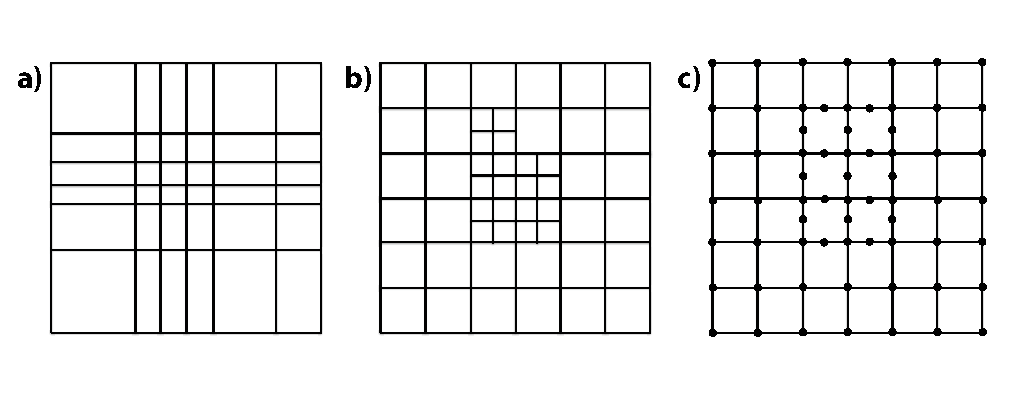
\includegraphics[width=\textwidth,height=\textheight,keepaspectratio]{Intro/refinement_types.eps}}
   \caption{Simplified examples of adaptive refinement techniques: (a) \emph{r}-refinement ---
    The number of grid cells is held constant, but the spacing between them changed,
    (b) \emph{h}-refinement --- the number of grid cells is increased by subdividing the grid, and
    (c) \emph{p}-refinement --- the polynomial order on the sub-grid scale is increased over the area of interest. The black
    dots represent the nodes in each grid cell.
   }
   \label{fig:refinetypes}
\end{figure}

   \subsubsection{r-refinement}
   In \emph{r}-refinement, the grid topology and number of grid elements remain unchanged;
instead, the elements are dynamically redistributed to increase resolution in parts of the grid 
while decreasing it everywhere else (Fig. \ref{fig:refinetypes}a). This dynamic mesh 
redistribution creates smoother transition regions between resolutions but
requires a complex global remapping of the mesh to move the location of the high 
resolution. The number of refined areas that can be formed are limited, and if the 
remapping transformation algorithms are not carefully constructed, grid tangling problems
and convergence issues can arise \citep{budd2009adaptivity}. \emph{r}-refinement is the 
dynamic version of static stretched grids.

In an early application of \emph{r}-refinement, \cite{Dietachmayer:1992sj} and 
\cite{dietachmayer1992application} used this global grid redistribution
technique to increase resolution in areas where the estimated solution
error is high. \cite{giraldo2000lagrange} and
\cite{iselin2002dynamic} applied this type of dynamic
adaptation for the 2D shallow water equations and advection problems,
respectively. More recently, \cite{Walsh:2010om} studied  
two-dimensional baroclinic instability with \emph{r}-refinement and
\cite{kuhnlein2012modelling} implemented \emph{r}-adaptivity within a 3D
Cartesian framework. \cite{bauer2014simulation} used \emph{r}-refinement grids guided by
error estimates in a shallow water model, and
\cite{weller2016mesh} demonstrated \emph{r}-refinement use on the
sphere.

   \subsubsection{h-refinement: Adaptive Mesh Refinement}
   Adaptive mesh refinement (AMR), also known as \emph{h}-refinement, increases resolution 
locally either by adding cells within the grid structure or by overlaying additional cells of finer 
resolution on top of the grid without changing the base grid structure (Fig. \ref{fig:refinetypes}b). 
Nested grids are the comparable static refinement technique.
            
\cite{skamarock1989adaptive} and
\cite{skamarock1993adaptive} implemented AMR by placing finer-resolution
meshes over the coarse grid in areas which had large truncation error
estimates. The grid-cell solutions and boundary conditions between the
finer-resolution meshes and the base grid are continually updated.  In
a more recent example,
\cite{Chen:2011kk} use AMR to overlay high-resolution meshes in areas
of interest in a shallow water model on a cubed-sphere grid.

Examples of AMR techniques which locally add and remove cells to the base
grid for the shallow water equations on the sphere have been presented
by
\cite{behrens2005amatos},
\cite{lauter2007parallel},
\cite{st2007comparison} and
\cite{marras2015simulation}.  Both
\cite{behrens2005amatos} and
\cite{lauter2007parallel} use conformal unstructured finite element
meshes.  In conformal grids, each cell shares an edge with exactly one
other cell, while in a non-conforming grid, cells can share an edge with
more than one neighboring element (Fig. \ref{fig:conform_noncon}).
Conformal grids can maintain conservation properties easily, avoid possible
discontinuities at refinement boundaries, and provide smoother transitions.
Non-conformal grids can provide more flexible refinement capabilities and, 
with simpler computational grid structures, run more efficiently on
large parallel supercomputers \citep{jablonowski2009block}.
The two AMR models described in
\cite{st2007comparison}, a block-structured finite-volume method on a
latitude-longitude grid and a spectral-element method on a cubed-sphere
grid, use nonconforming meshes and a quad-tree based AMR method with
gradient- or vorticity-based refinement criteria.
\cite{marras2015simulation} compared the use of an AMR approach on
several structured and unstructured non-conformal grids.  

\begin{figure}
   \centerline{%
   \noindent
   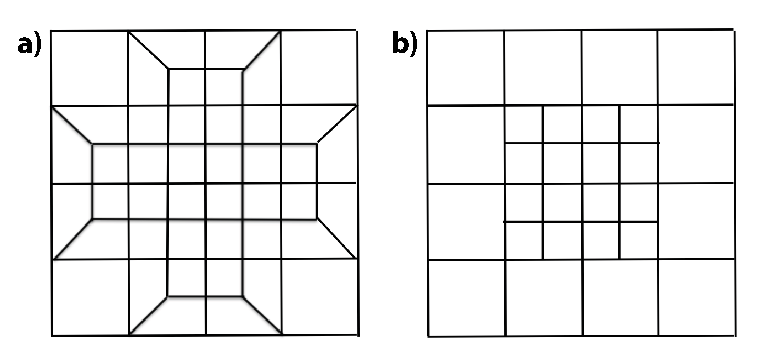
\includegraphics[width=\textwidth,height=\textheight,keepaspectratio]{Intro/mapping-conform.eps}}
   \caption{(a) Conformal grid --- each cell shares an edge with exactly one other cell and
    (b) Non-conformal grid --- cells can share an edge with more than one neighbor, 
    which results in hanging nodes.
   }
   \label{fig:conform_noncon}
\end{figure}

Use of AMR in a
regional model paired with a physical parameterization package was
presented in \cite{bacon2000dynamically}. OMEGA has been 
tested in forecasting hurricane storm tracks \citep{bacon2007hurricane}.
AMR methods have also been investigated for 
2D flow fields in Cartesian geometry. Recent examples include 
\cite{muller2013comparison} and \cite{kopera2014analysis} 
who analyzed a tree-structured AMR algorithm for 
non-hydrostatic dynamical cores in the x-z plane, and  
\cite{hendricks2016evaluation} who explored static and dynamic AMR for 
tropical-cyclone-like vortices in a shallow water model 
on an $f$-plane with a constant Coriolis parameter $f$.

   \subsubsection{p-refinement: Adaptive Order Refinement}
The third type of dynamic refinement, \emph{p}-refinement, holds the
grid spacing fixed but changes the order of the polynomial approximation
within each grid element to increase local resolution. Use of \emph{p}-refinement
with Discontinuous Galerkin (DG) methods for the shallow water equations
were described by \cite{kubatko2009dynamic} and
\cite{tumolo2015semi}. For smooth problems, \emph{p}-refinement offers a high rate of 
convergence with significantly less computational expense than other refinement types, 
but it has difficulty resolving sharp gradients in the flow field. To ameliorate these problems,
a hybrid refinement method that combines the
\emph{h}- and \emph{p}-refinements methods was demonstrated by
\cite{eskilsson2011hp}. \cite{blaise2012dynamic} used an \emph{hp}-adaptive DG method to model
the shallow water equations on a sphere for global tsunami
simulations and \cite{kopera2014analysis} implemented an DG method with \emph{hp}-refinement
in a two dimensional $xz$-projection of the compressible Euler equations.

\section{Challenges associated with dynamic refinement}
It has been nearly 30 years since the first adaptive atmospheric models 
were published \citep{skamarock1989adaptive,Dietachmayer:1992sj}.  Static refinement has been used for decades 
in regional weather models and VRGCMs have become a growing fixture in global climate modeling.  
Adaptive refinement for atmospheric modeling has remained mostly an academic exercise, 
with recent development centered on testing various refinement techniques in idealized one 
and two dimensional systems. Modeling the atmosphere is a far more complex problem 
than current applications of dynamic refinement as features of interest are more diverse and less 
well defined. To that end, there are several ongoing challenges that need to be addressed for AMR
to become a tool for climate and weather modeling. 

The key issue that most recent dynamical refinement work has been seeking to address is
the development of robust numerical methods that run efficiently on today's supercomputers.
A continuously changing grid structure sharply increases the difficulty in developing
numerical schemes that are efficient, accurate, and stable.
Dynamic refinement models still need to be locally conservative, preserve monotonicity, 
and minimize and manage numerical artifacts that arise from the grid refinement structure. 
Furthermore, any method must preserve consistency in the full equation sets. 
For example, at around 10 km resolution the hydrostatic approximation is no longer valid and models
need to solve the more complex full non-hydrostatic equations. 

Adaptive methods present more challenges for running simulations 
on current massively parallel supercomputers than traditional
static models face.  The processor and memory requirements of a dynamic refinement 
model change as grid elements are added and removed. Dynamic refinement techniques 
also use complex data structures requiring more computational overhead to organize
the grid elements and communicate the grid changes.
For dynamic refinement methods to become more 
mainstream, they need to be more computationally efficient than current uniform models yet generate the same accuracy and skill. 
Both the block-structured \citep{jablonowski2009block,Chen:2011kk} and unstructured quad-tree refinements \citep{lauter2007parallel,blaise2012dynamic} show promise as methods that ensure computationally efficient refinement on high performance computing platforms.

Another issue facing both dynamic and static VRGCMs is scale-aware physics parameterizations. 
In current uniform climate and weather models, the physics schemes that approximate the
unresolved and sub-grid scale processes are specifically tuned to the model's resolution. 
Increasing resolution without re-tuning the physics parameterizations can adversely affect
results \citep{rauscher2013exploring,zarzycki2014aquaplanet}. So, in adaptive schemes, 
the sub-grid parameterizations need to be able to adjust for changes in scale.  
A model would need to be able to phase out certain sub-grid processes, like deep
convection, as resolution is increased and these processes are resolved on the actual mesh.
Several parameterization schemes (e.g. the newly developed cloud scheme 
Cloud Layers Unified By Binormals (CLUBB) in the National Center for Atmospheric Research's
Community Atmosphere Model) are being designed to work with varying vertical and horizontal resolutions.

A final issue in dynamic refinement is the selection of refinement criteria that determine where refinement is added.
If a refinement criterion is too selective, key features will not be refined; if a criterion is too relaxed, 
refinement areas will become too large, making the model inefficient. Furthermore, the multiscale nature 
of the atmosphere and its interconnectivity creates a plethora of refinement criteria possibilities 
such that one set of criteria will not work effectively on all possible features of interest. Thus finding criteria 
that detect the areas that need to be refined as accurately and efficiently as possible is vital for 
effective implementation of adaptive meshes. A variety of criteria have been proposed and tested
in the literature including local error estimates 
\citep{skamarock1989adaptive,lauter2007parallel,bauer2014simulation} and physical
variables like pressure or wind \citep{bacon2000dynamically,st2007comparison,kopera2014analysis}.

Global dynamic refinement models retain potential as powerful tools for 
solving complex, nonlinear, multiscaled weather and climate systems.  
 Dynamic refinement could benefit many applications involving transient 
localized phenomena including tropical cyclones, atmospheric blocking events, orographic 
precipitation, and pollution dispersion. Even long-term climate simulations could benefit as 
localized flow structures may be important in determining climate signals, such as modeling
atmospheric rivers on the West coast of the United States.  

\section{Outline of Thesis}
This thesis presents ongoing work to implement AMR within 
a new nonhydrostatic, finite-volume dycore and to demonstrate 
AMR's effectiveness in improving model accuracy and 
resolving multiscale features. These efforts are accomplished by 
implementing a hierarchy of new and existing test cases of increasing 
complexity for the 2D shallow water and 3D non-hydrostatic equations. 
The thesis is organized as follows. In Chapter \ref{chap:basicsw} we implement existing 
shallow water test cases and develop several new ones to assess 
the capabilities of AMR in the shallow water version of the 
\cite{mccorquodale2015adaptive} finite volume Chombo AMR 
model. The results of this research were published in \cite{ferguson2016analyzing}.
Chapter \ref{chap:forcedsw} presents two different 
forced shallow water systems with moisture variables designed to 
represent convective and precipitation processes as more challenging 
testbeds to use with the finite volume Chombo AMR model. In 
Chapter \ref{chap:3dmodel}, we investigate the effects of AMR using 
the 3D non-hydrostatic version of the finite-volume Chombo AMR model in 
two 3D test cases. The first consists of a simple dry flow without 
forcing while the second adds a simplified physics parameterization 
scheme. Conclusions and future directions are presented in Chapter \ref{chap:conclusion}.
 
%  \chapter{Model Description}
% \label{chap:model}
% \section{non-hydrostatic finite volume Chombo AMR model on the cubed sphere}
Discuss hydrostatic vs non-hydrostatic

\section{Governing Equations}

The flux form of the shallow water equations is:
\begin{equation}
	\frac{\partial h\mathbf{u}}{\partial t}+\nabla\cdot(\mathbf{u}h\mathbf{u})=-f\mathbf{\hat{k}}\times h\mathbf{u}-Gh\nabla H
\end{equation}
\begin{equation}
	\frac{\partial h}{\partial t}+\nabla\cdot(h\mathbf{u})=0
\end{equation}
where $H=h+z_{s}$ with $h$ the fluid height and $z_{s}$ the height of the underlying topography. $\mathbf{u}$ is the velocity vector, and $\mathbf{\hat{k}}$ is the unit vector perpendicular to the surface.  The Coriolis parameter is $f$ while $G$ is the gravitational acceleration constant. In equiangular coordinates, the shallow water equations on a cubed sphere can be written as:
\begin{equation}
     \label{eq:SWcubesphere}
     \frac{\partial}{\partial t}\left(J\mathbf{U}\right) + \nabla\cdot(J\mathbf{\vec{F}}) = J\mathbf{\Psi}
\end{equation}
where
\begin{equation}
      \mathbf{U}= \left( \begin{array}{c}
       h \\
       h u^\alpha \\
       h u^\beta
       \end{array} \right), \
       \mathbf{F}^k = \left( \begin{array}{c}
        h u^k \\
        hu^{k}u^{\alpha}+g^{k \alpha}\frac{1}{2}Gh^{2} \\
        hu^{k}u^{\beta}+g^{k \beta}\frac{1}{2}Gh^{2} 
        \end{array} \right), \
        \mathbf{\Psi} =  \left( \begin{array}{c}
        0 \\
        \mathbf{\Psi}_{M}^{\alpha}+\mathbf{\Psi}_{C}^{\alpha}+\mathbf{\Psi}_{B}^{\alpha} \\
        \mathbf{\Psi}_{M}^{\beta}+\mathbf{\Psi}_{C}^{\beta}+\mathbf{\Psi}_{B}^{\beta} \\
         \end{array} \right).
\end{equation}
Here $\mathbf{U}$ contains the conserved variables while the first term in $\mathbf{F}^{k}$ is the "mass" flux vector and the bottom two terms are the "momentum" flux tensors.  $J$ is the Jacobian on the manifold and $g^{nk}$ is the contravariant cubed sphere metric with $k$ and $n$ $=\{\alpha,\beta\}$.  The $\mathbf{\Psi}_{M}$, $\mathbf{\Psi}_{C}$, and $\mathbf{\Psi}_{B}$ terms represent the metric, Coriolis, and bottom topography source terms respectively (See \cite{McCorquodale:2014rw} for the full representations of the source terms). 

In three dimensions very similar.

\section{The cubed-sphere grid}
The cubed-sphere grid was developed by \cite{Sardony} as a solution to the "pole problem" that traditional spherical latitude-longitude grids 
possess. In the latitude-longitude  projection, converging meridians create singularities at North and South poles with computationally inefficient 
small grid spacing near the poles. The cubed-sphere grid avoids this "pole-problem" by projecting a gridded cube onto the surface of a sphere. The grid replaces the two strong singulars of poles with eight weaker singularities at
the corner points of the originally cube.  The cubed-sphere grid also provides a near uniform tiling of the sphere compared with the
large changes in grid spacing on the latitude-longitude mesh. However, the grid design
was not competitive with existing models as the overhead cost of storing the grid structure computationally
were too significant. The use of the cubed-sphere was revived in the mid 1990s in a shallow water 
model by \cite{Ronchietal}. Since then the cubed-sphere grid has been implement in several shallow water models and 
a few full atmospheric
models including the hydrostatic Community Atmosphere Spectral Element Model (CAM-SE) \citep{dennis2012cam}, the
non-hydrostatic Tempest model \citep{ullrich2014global,guerra2016high}, and the
Geophysical Fluid Dynamics Laborator's Finite-Volume Cubed-Sphere Dynamical Core (FV3) \citep{lin2004vertically,Harris:2013n}.
In 2016, the National Weather Service selected the cubed-sphere FV3 dynamical core to be implemented in the new version
of the Global Forecast System, its main weather forecast model, which will be operational in 2019.
This growth in use of the cubed sphere grids is a result of the develop of massively
parallel computing systems on which GCMs can now be ran. 
The regular grid structure on each panel allows the computational grid to be efficiently distributed
across these large parallel systems. This regularity also allows additional grid cells to be added or 
removed for variable resolution with more ease compared to unstructured geodesic (icosahedral) grids or the 
more complex Yin-Yang grid.

\begin{figure}[htp]
\centerline{
\includegraphics[width=4in]{ModelDescription/cubedsphere12456.pdf} % was cubedsphere2dreal                                                                                        
}
\caption{
A cubed-sphere grid, shown with labels on panels.
% The surface of the unit sphere in real space.                                                                                                              
Panels 1 -- 4 all straddle the equator
($z = 0$) of the unit sphere.
Panel 5 is centered on the north pole ($z = +1$),
panel 6 on the south pole ($z = -1$).
On the cubed-sphere grid shown here,
$N_{\rm c} = 16$ (each panel contains $16 \times 16$ grid cells).
}
\label{fig:cubedsphere2dmaps}
\end{figure}

The cubed-sphere grid consists of cubed with six Cartesian panels inflated out to form a spherical shell. 
There are multiple ways to map the grids of each panel to the sphere (see \cite{Putnam:2007cs} for a review
of several cubed sphere grids).  The Chombo-AMR model uses gnomonic equiangular cubed-sphere grid, where the
gridlines on each panel have equally spaced central angles relative to the center of the sphere. This projection
gives a quasi-uniform spherical grid. The gird does not have perfectly uniform grid sizes, but as resolution increases
the ratio between the largest and smallest grid cells converges to $\sqrt{2}$, the smallest ratio of cubed-sphere
grids. Figure \ref{fig:cubedsphere2dmaps} depicts the equiangular cubed-sphere grid.

The equiangular coordinates for the cubed-sphere grid are given as $(\alpha, \beta, n_p)$, 
with central anngles $\alpha, \beta \in [-\frac{\pi}{4},\frac{\pi}{4}]$ and the panel number $n_p \in [1,2,\dots, 6]$. 
By convention, panels 1-4 are along the equator and panels 5 and 6 are centered on the north and south poles
respectively as seen Fig. \ref{fig:cubedsphere2dmaps}. The discrete resolution of the cubed-sphere grid is represented as  $c\{N_c\}$ where $N_c$
denotes the number of grid cells in each direction on the six panels.  A
list of properties of the equiangular cubed-sphere grid, including the
approximate grid spacings, and comparable resolutions for other coordinate systems, is given in
Table~\ref{tb:grids} for several resolutions.

\begin{table}[t]
    \caption{Properties for several cubed-sphere grid resolutions where 
    $N_c$ is the number of cells along an edge of a cubed-sphere panel.
    Here the number of cells is the total number of grid cells 
    ($N_c^2 \times 6$), $\Delta x$ is the approximate grid spacing, 
    $A_{avg}$ is the average area of a grid cell, $A_{min}/A_{max}$ is the
    ratio between the minimum and maximum cell areas, Eq.  Res.  is the
    grid resolution in degrees given by $90^\circ / N_c$, and $RLL_{equiv}$
    is the equivalent grid spacing on a regular latitude-longitude
    grid with the same total number of cells.}%
    \label{tb:grids}
    \begin{center}
    \begin{tabular}{cccrccc}
            \hline
            Resolution ($N_c$) & No. of cells       & $\Delta x$ (km) & $A_{avg} (\mbox{ km}^2)$ & $A_{min}/A_{max}$ & Eq. Res.     & $RLL_{equiv}$ \\ 
            \hline
            \hline
            c$32$              & $6.14 \times 10^3$ & $313$           & $8.302 \times 10^{4}$    & $0.7249$          & $2.81^\circ$ & $3.25^\circ$  \\ 
            c$64$              & $2.46 \times 10^4$ & $156$           & $2.076 \times 10^{4}$    & $0.7159$          & $1.41^\circ$ & $1.62^\circ$  \\ 
            c$128$             & $9.83 \times 10^4$ & $78.2$          & $5.189 \times 10^{3}$    & $0.7115$          & $0.70^\circ$ & $0.82^\circ$  \\ 
            c$256$             & $3.93 \times 10^5$ & $39.1$          & $1.297 \times 10^{3}$    & $0.7093$          & $0.35^\circ$ & $0.41^\circ$  \\ 
            c$512$             & $1.57 \times 10^6$ & $19.5$          & $3.243 \times 10^{2}$    & $0.7082$          & $0.18^\circ$ & $0.20^\circ$  \\ 
            c$1024$           & $6.29 \times 10^6$ & $9.77$          & $8.107 \times 10^{1}$    & $0.7076$          & $0.09^\circ$ & $0.10^\circ$  \\ 
            c$2048$           & $2.52 \times 10^7$ & $4.89$          & $2.027 \times 10^{1}$   & $0.7074$          & $0.04^\circ$ & $0.05^\circ$ \\
            \hline
        \end{tabular}
    \end{center}
\end{table}

%%%%%%%%%%%%%%%%%%%%%%%%%%
\section{Finite Volume Discretization}
Finite-volume methods were first developed in 
other areas of hydrodynamics such as astrophysics 
and aerospace for modeling high speed flows and shockwaves and 
trace their origins back to the conservative finite-volume methods developed
by \cite{Godunov}. These methods were extend to second order by the work of Bram
van Leer in \cite{van Leer}
and later \cite{Collela} developed the piecewise-parabolic method (PPM), a third-order
Godunov-type finite volume method.
Early adaptations of finite-volume methods for atmospheric advection problems
by \cite {rood 1987}, \cite{Carpenter et al. (1990)}, and \cite{Allen1991} led to the development 
a finite-volume dynamical core for the shallow water equations \citep{Lin Rood} and later the full 3D
equations of motion \citep{Lin2004}
Use of finite-volume methods in GCMs has grown, especially with the development of variable resolution. Recently developed models that utlize a finite volume dynamical core include GFDL's FV3, NCAR's Model for Prediction Across Scales (MPAS), and Max-Planck-Institut's ICOsahedral Non-hydrostatic model.
A key advantage of finite volume methods is that they are conservative so they can preserve properties like mass and maintain high accuracy. Additionally, finite-volume methods can be easily formulated for moving or adaptive meshes.

  The finite volume dynamical core uses a volume integral formulation of the equations of motions. 
       In the finite volume approach to discretizing the non-hydrostatic equations, we integrate the equations of motions over the 
       volume of a grid cell
       The Chombo-AMR model uses a conservative 4th order finite-volume scheme to solve the shallow water equations.  Applying a method-of-lines approach, we integrate the SWEs (Equation \ref{eq:SWcubesphere}) over grid cell $V_{i,j}$, make use of Gauss' divergence theorem, and represent the integrals in terms of averages over $V_{i,j}$ and its faces to obtain the discretized volume averaged formulation: 
       \begin{align}
       \frac{d}{dt} \langle J \mathbf{U} \rangle_{i,j}
       = & - \frac{1}{\Delta \alpha} 
       \left( \langle J \mathbf{F}^\alpha \rangle_{i + \frac{1}{2},j} -
       \langle J \mathbf{F}^\alpha \rangle_{i - \frac{1}{2},j} \right)
      - \frac{1}{\Delta \beta}
      \left( \langle J \mathbf{F}^\beta \rangle_{i,j + \frac{1}{2}} -
      \langle J \mathbf{F}^\beta \rangle_{i,j - \frac{1}{2}} \right)
      + \langle J \mathbf{\Psi} \rangle_{i,j} .
      \label{eqn:PDEAveraged}
      \end{align}
 where $\Delta\alpha=\Delta\beta=\frac{\pi}{2N_c}$ are the grid spacing on the equiangular grid, $\langle A \rangle_{i,j}$ represents the average of a quantity $A$ over $V_{i,j}$, and $\langle A \rangle_{i \pm \frac{1}{2},j \pm \frac{1}{2}}$ denote the averages over the faces of $V_{i,j}$,.

   The fluxes at the faces of each grid cell are then obtained via a complex centered spatial interpolation involving deconvolving, interpolating and then convolving the cell values to maintain 4th order accuracy (see \cite{McCorquodale:2014rw} for a full description).  Ghost cells are created by interpolating from stencils of nearby cells (Figure \ref{fig:ghostcellstens}) at boundaries between panels and between block-structures of different resolutions.  
   \begin{figure}[h]
   \centerline{ 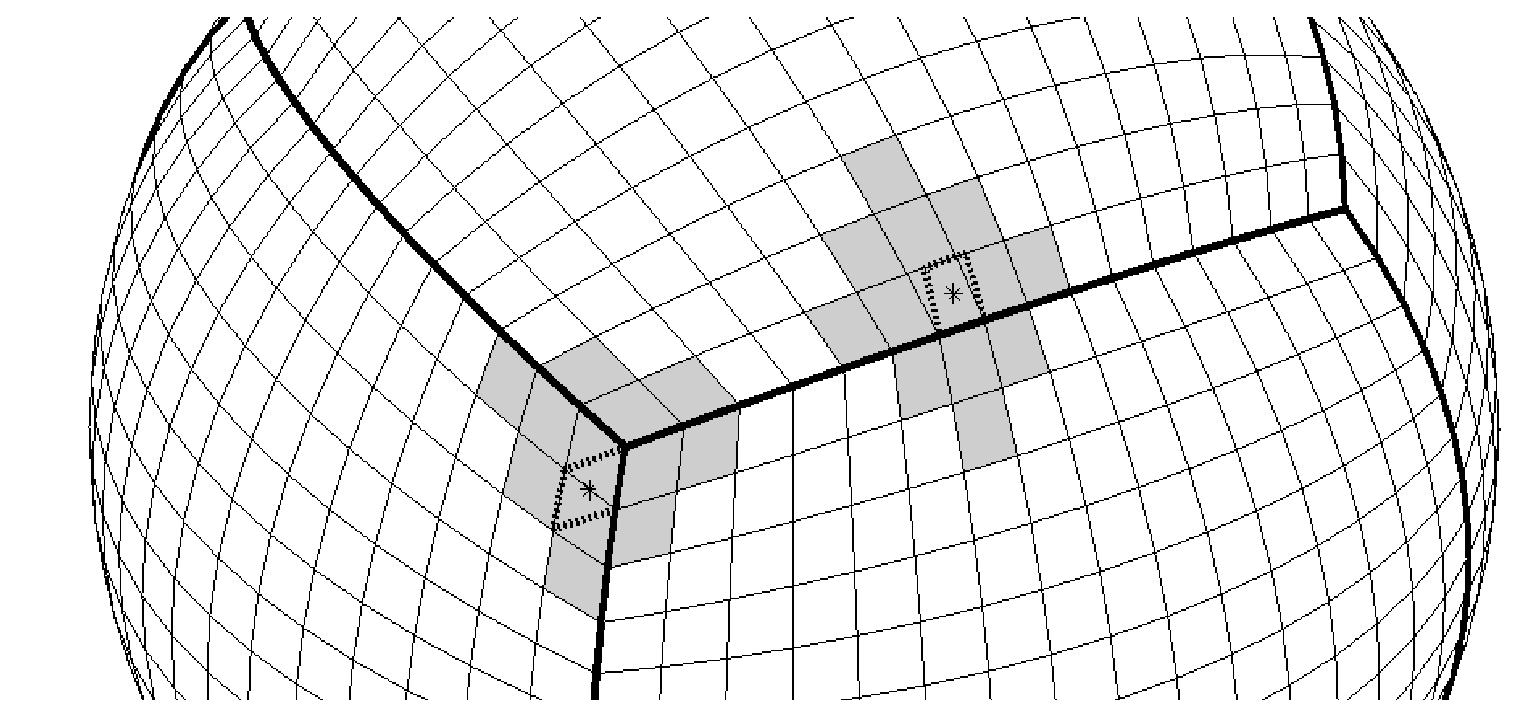
\includegraphics[width=.7\textwidth]{ModelDescription/CSstencilUniform} }
   \caption{Sample interpolation stencils (shaded cells) of two different ghost cells marked with a * at the boundaries of a panel.}
   \label{fig:ghostcellstens}
   \end{figure}
   
   A classical fourth-order explicit Runge-Kutta method is used to advance Equation \ref{eqn:PDEAveraged} in time, which can be written in the form
   \begin{align}
      \frac{d}{dt} \langle J \mathbf{U} \rangle_{i,j}
       = K ( \langle J \mathbf{U} \rangle )_{i,j}
       \label{eqn:PDEAveragedK}
   \end{align}
   such that $K\left(\langle J\mathbf{U} \rangle\right)_{i,j}$ equals the right hand side of Equation \ref{eqn:PDEAveraged}.  Integrating Equation \ref{eqn:PDEAveragedK} over time step $\Delta t$  using the classical Runge-Kutta method with $\langle J \mathbf{U} \rangle^{(0)}$ as the initial value gives the following equations:
   \begin{align}
      & & k_1 & = K(\langle J \mathbf{U} \rangle^{(0)} ) \Delta t; \label{eqn:k1} \\
      \langle J \mathbf{U} \rangle^{(1)} & = \langle J \mathbf{U} \rangle^{(0)} + \frac{k_1}{2} ; &
      k_2 & =   K(\langle J \mathbf{U} \rangle^{(1)} ) \Delta t; \label{eqn:k2} \\ 
      \langle J \mathbf{U} \rangle^{(2)} & = \langle J \mathbf{U} \rangle^{(0)} + \frac{k_2}{2} ; &
      k_3 & =  K(\langle J \mathbf{U} \rangle^{(2)} ) \Delta t; \label{eqn:k3} \\
      \langle J \mathbf{U} \rangle^{(3)} & = \langle J \mathbf{U} \rangle^{(0)} + k_3 ; &
       k_4 & = K(\langle J \mathbf{U} \rangle^{(3)} ) \Delta t \label{eqn:k4} 
    \end{align}
    so that the solution at $t+\Delta t$ is
    \begin{equation}
        \langle J \mathbf{U} \rangle(t^n + \Delta t) = 
        \langle J \mathbf{U} \rangle(t^n) + \frac{1}{6} (k_1 + 2 k_2 + 2 k_3 + k_4) +
        O((\Delta t)^5).
    \end{equation}
    
%%%%%%%%%%%%%%%%%%%
\section{Chombo AMR framework}
The adaptive mesh refinement (AMR) is based on the Chombo library for parallel AMR.   The Chombo library provides a set of tools for finite-difference and finite-volume methods for solving partial differential equations on block-structured AMR grids \citep{colella2000chombo}.  It is a highly-scalable solver that has been shown to scale to $\mathcal{O}(10^{5})$  processors for hyperbolic and elliptical equations related to gas dynamics.    The AMR structure allows refinement around an unlimited number of targeted features and at various levels of refinement. 
   
    AMR calculations are performed on a hierarchy of nested-mesh levels, with a predefined refinement ratio (e.g. 2, 4, or 8) between adjacent levels.  An intermediate level must have enough cells separating the finer and coarser levels to allow interpolation of ghost cells for the finer level.  Levels are grouped into sections of grid cells, called "boxes", in order to perform calculations on large parallel platforms efficiently.  Figure \ref{fig:test1} shows a sample layout of refinement levels and boxes.  AMR grid levels are advanced in time through a sub-cycling process.  The process is outlined in Figure \ref{fig:timesubcycle} (see \cite{McCorquodale:2014rw} again for full details).
        \begin{figure}[h]
 		\centering
  		\includegraphics[width=.6\linewidth]{ModelDescription/amr_block_example}
  		\caption{From \cite{GuzikETAL:2013}, this figure shows a three level grid hierarchy with a x2 refinement ratio between levels.  The block structure is depicted by bolded lines.  Note that the finest layer is nested within the middle layer to allow for the interpolation of ghost cells.  Ghost cells for the middle layer are shown by dashed lines.}
  		\label{fig:test1}
	\end{figure}
	
	\begin{figure}[h]
 		\centering
  		\includegraphics[width=.8\linewidth]{ModelDescription/Time_subcycle_chart}
  		\caption{This diagram depicts the time advancement processes for AMR. The $l$ level is advanced first.  Ghost cells for the $l+1$ level are interpolated both at time $t$ and then from intermediate time steps. The $l+1$ level is then advanced, forward in time; and once a sub-cycle is complete, averages and fluxes are updated back to the coarser level.  This process is cascaded down to the highest refinement level.  The order in which levels are advanced through the sub-cycling is shown by the black arrows.}
 		 \label{fig:timesubcycle}
	\end{figure}
    
    New levels are added whenever the refinement criteria are reached at the current level.  The mesh can be refined up to a predefined number of levels.   AMR-Chombo has a range of possible refinement criteria.  Currently it can base refinement on the gradient or absolute value of vorticity, height, a tracer field, and topography.    The criteria can be set to increase with refinement level or remain constant.  For example, the c256 level would have to observe a higher vorticity than the c64 level to refine further.  Furthermore, new refinement criteria can easily be created and implemented. 
    
%%%%%%%%%%%%%%%%%%%
\section{Shallow Water model setup}


Because the shallow-water equations mimic atmospheric flow in a single layer, 
they serve as a common test bed for atmospheric model development. The shallow-
water equations describe the behavior of a homogenous, incompressible, 
and inviscid fluid in a shallow layer. While sound waves are not supported, the shallow-
water equations are able to resolve Kelvin, Inertia-Gravity, and non-linear 
Rossby waves. By capturing these key wave 
propagations mechanisms, the shallow-water equations retain some of the
most pertinent dynamical features found in the real atmosphere and in 
full three dimensional atmospheric GCMs while staying relatively simple enough to enable 
detailed investigations of a model's dynamical components. A shallow-water model provides
a basic test of horizontal and temporal discretization schemes to determine which numerical
schemes are effective for atmospheric flows without requiring the effort of building a complete
complex model. With the extensive use shallow water models, a wide range test cases have
been developed for the shallow-water equations to evaluate various characteristics of the numerical
schemes. Test cases serve as a useful comparison benchmarks with existing models to 
determine the effectiveness of new numerical technics.
Many test cases consists of simple artificial 
flows with analytical solutions while others have more complex realistic flows without 
an analytic solution and use high resolution runs from existing models as a comparison.
Common test cases implemented in today's literature included
the now canonical test case suite of \cite{Williamson:1992kx} as well as more recently
developed tests including the barotropic instability of \cite{Galewsky:2004uq}. In
our assessment of the AMR model, we implement several established test cases and also
develop several new ones.


\section{3D Model setup}


 \chapter{Adaptive mesh refinement in 2D advection and shallow-water simulations}
 \label{chap:basicsw}
 \section{Introduction}
\label{sec:introduction}
Global climate models have become vital tools for
simulating the present and future climate and for predicting important
climate trends.  However, current global models are limited in their
ability to represent many multi-scale aspects of atmospheric flows.
Their resolutions, limited by computational costs, are too coarse to
accurately represent key processes that span a wide range of temporal
and spatial scales.  High-resolution simulations are essential for
capturing these scale interactions and for accurately representing local
and regional phenomena such as convection, orographically induced
precipitation, mesoscale storm systems, and tropical cyclones.  Such
events have large regional impacts as well as broader feedbacks onto the
large-scale climate system.  Today, high-resolution General Circulation
Models (GCMs) used for global climate simulations can utilize uniform
grid spacings down to 10 km as documented by, e.g.,
\cite{manganello:12} or
\cite{kinter:13}.  However, they are computationally very expensive and
still unable to represent key processes such as clouds explicitly.
Exceptions are the cloud-permitting, partly cloud-resolving, global
simulations by
\cite{miura:07},
\cite{putman:11} or
\cite{miyamoto:13} that were run for short, multi-day time periods with
grid spacings in the 0.9--3.5 kilometer range.  To employ such high
resolutions over longer climate time periods, modelers typically use
limited-area models (LAMs) that focus the computational resources in
areas of interest.  A major drawback is that LAMs require their lateral
boundaries to be externally forced.  These boundary conditions are
typically derived from much coarser GCMs which use different numerical
schemes and physical parameterizations, thereby introducing possible
biases or numerical discrepancies.  In addition, it is an open question
how well LAMs can capture teleconnections of global large-scale dynamics
and localized features particularly for tropical cyclones and other
phenomena that have feedbacks onto the larger climate system.

Variable-resolution GCMs can utilize static or dynamic grid
refinements which are promising options to bridge the gap between global
and regional climate modeling.  Application examples for static (non-moving)
mesh adaptations are provided in, for example,
\cite{zarzycki2014using}, \cite{rauscher2014impact}, \cite{zarzycki2015tropical} and
\cite{huang:16} (see also further references therein).  This chapter
focuses on dynamically adaptive grids, which track features of interest
during the model simulation by locally adding or removing grid points as
needed.  Adaptation criteria based on error estimates (e.g.
\cite{skamarock1989adaptive},
\cite{behrens1998atmospheric}, and
\cite{blaise2012dynamic}) or flow characteristics (e.g.
\cite{hubbard2003three}, 
\cite{jablonowski2006AMR,jablonowski2009AMR} and
\cite{st2007comparison}) can be used to determine
where the high-resolution mesh should be placed.  By increasing
resolution only locally, dynamic refinement significantly decreases the
total number of degrees of freedom for the simulation.  However, since
dynamic refinement is used within a global model, it also eliminates the
need for forced boundary conditions and solves the local high-resolution
area and global flow using the same dynamical core and physics package.
Global models allow for a better representation of global and
synoptic-scale phenomena and permit them to interact better with meso-
and small-scale features that can be resolved in the model.
Additionally, a key advantage of dynamic refinement compared to a static
refinement setup is that the location of the refined area does not have
to be determined \emph{a priori}.  

Adaptive refinement methods are
well established in many areas of computational fluid dynamics like aerospace engineering or 
space weather modeling (see e.g. \cite{toth2012adaptive}). In atmospheric science though, the
costs and benefits of AMR methods have mostly been
evaluated in idealized simulations and simplified models so far.  
Some of the first adaptive atmospheric models were developed by
\cite{skamarock1989adaptive},
\cite{skamarock1993adaptive}, and
\cite{Dietachmayer:1992sj}.  In general, the grid refinement strategies can be
categorized into three overarching types:  \emph{r}-refinement (or \emph{r}-adaptivity),
\emph{h}-refinement, and \emph{p}-refinement.

In \emph{r}-refinement, the number of grid cells remains unchanged;
instead, the cells are dynamically redistributed to increase resolution
in parts of the grid while decreasing it everywhere else.  This dynamic
grid adaptation creates smoother transition regions between resolutions but
requires a complex global remapping of the mesh to move the location of
the high resolution.
\cite{Dietachmayer:1992sj} uses this global grid redistribution
technique to increase resolution in areas where the estimated solution
error is high.
\cite{giraldo2000lagrange} and
\cite{iselin2002dynamic} have also applied this type of dynamic
adaptation for the 2D shallow-water equations and advection problems,
respectively.  More recently,
\cite{kuhnlein2012modelling} implemented \emph{r}-adaptivity within a 3D
Cartesian framework,
\cite{bauer2014simulation} used \emph{r}-refinement grids guided by
error estimates in a shallow-water model, and
\cite{weller2016mesh} demonstrated \emph{r}-refinement use on the
sphere.

Adaptive mesh refinement (AMR),
another term for \emph{h}-refinement,
increases resolution locally either by adding cells within the grid
structure or by overlaying additional cells of finer resolution on top
of the grid without changing the base grid structure.
\cite{skamarock1989adaptive} and
\cite{skamarock1993adaptive} implemented AMR by placing finer-resolution
meshes over the coarse grid in areas which had large truncation error
estimates.  The grid-cell solutions and boundary conditions between the
higher-resolution meshes and the base grid are continually updated.  In
a more recent example,
\cite{Chen:2011kk} use AMR that overlays high-resolution meshes in areas
of interest in a shallow-water model on a cubed-sphere grid.
Examples of AMR techniques that locally add and remove cells to the base
grid for the shallow-water equations on the sphere have been presented
by
\cite{behrens2005amatos},
\cite{lauter2007parallel},
\cite{st2007comparison} and
\cite{marras2015simulation}.  Both
\cite{behrens2005amatos} and
\cite{lauter2007parallel} use conformal unstructured finite element
meshes.  In conformal grids, each cell shares an edge with exactly one
other cell, while on a nonconforming grid, cells can share an edge with
more than one neighboring element.  The two AMR models described in
\cite{st2007comparison}, a block-structured finite-volume method on a
latitude-longitude grid and a spectral-element method on a cubed-sphere
grid, use nonconforming meshes and a quad-tree based AMR method with
gradient- or vorticity-based refinement criteria.
\cite{marras2015simulation} compared the use of an AMR approach on
several structured and unstructured non-conformal grids.  Use of AMR in a
regional model paired with a physical parameterization package was
presented in \cite{bacon2000dynamically}.
Furthermore, AMR methods have also been investigated for 
2D flow fields in Cartesian geometry. Recent examples include 
\cite{muller2013comparison} and \cite{kopera2014analysis} 
who analyzed a tree-structured AMR algorithm for 
non-hydrostatic dynamical cores in the x-z plane, and  
\cite{hendricks2016evaluation} who explored static and dynamic AMR for 
tropical-cyclone-like vortices in a shallow-water model 
on an $f$-plane with a constant Coriolis parameter $f$.

The third type of dynamic refinement, \emph{p}-refinement, holds the
grid spacing fixed but changes the order of the polynomial approximation
within each grid element to increase local resolution.  Use of \emph{p}-refinement
with Discontinuous Galerkin (DG) methods for the shallow-water equations
were described by \cite{kubatko2009dynamic} and
\cite{tumolo2015semi}.  A hybrid refinement method that combines the
\emph{h}- and \emph{p}-refinements methods was demonstrated by
\cite{eskilsson2011hp}, and
\cite{blaise2012dynamic} used an \emph{hp}-adaptive DG method to model
the shallow-water equations on the sphere for global tsunami
simulations.  Recently,
\cite{aechtner2015conservative} implemented a new adaptive wavelet
approach for local dynamic refinement with the 2D shallow-water
equations on the sphere.

The purpose of this study is to demonstrate the pros and cons of using
AMR, \emph{h}-refinement, for simulating atmospheric flows.
It assesses the effectiveness of AMR, employing a 
non-conformal grid, in achieving
similar results as uniform-grid simulations while reducing computational cost. Furthermore,
it is revealed that AMR can be implemented without harming or degrading the
large-scale smooth flows or inducing numerical noise and wave-like
reflections at AMR boundaries.  The 2D shallow-water equations serve as
a useful testbed for an AMR model as they exhibit many of the
complexities present in a full 3D model.  We utilize the cubed-sphere
fourth-order finite-volume AMR model presented in
\cite{mccorquodale2015adaptive} for the 2D shallow-water equations on
the sphere.  The model implements a mapped-multiblock AMR technique that
overlays refined patches on the coarser grid. Our work tests
the model's ability to track and refine over dynamic small-scale
features of interest and to evaluate refinement criteria.  We
investigate various refinement criteria, such as thresholds for the
height gradient or relative vorticity, that guide the locations of refinement
patches.  In addition, we shed light on factors that may limit AMR
applications including the size of the refinement ratios between grid
levels and the total number of levels.  Lastly, we examine the
effect of AMR on large relatively smooth flows where extra refinement is
unnecessary.  Specifically we focus on how the coarse-fine interfaces of
the AMR patches influence the overall flow and error.

The chapter is organized into three main sections.  A brief
description of the model and a discussion of the multiblock AMR
techniques are provided in Section~\ref{sec:model}.
Section~\ref{sec:results} discusses the results of the numerical tests.  One advection test and four
shallow-water tests are presented.  The tests are the moving vortices
advection test by \cite{Nair:2008fk}, a steady-state geostrophic flow
(test case 2 from \cite{Williamson:1992kx}), the unsteady solid body rotation test of
\cite{Lauter:2005uq}, a shallow-water test consisting of a gravity wave
impinging on an isolated mountain, and lastly a test that assesses the
interaction of idealized binary vortices.  Conclusions are provided in
Section~\ref{sec:conclusion}.

\section{Model Description}
\label{sec:model}

The Chombo-AMR dynamical core (dycore) is a new model that is built upon
an unstaggered high-order finite-volume (FV) multiblock approach with a
classical fourth-order Runge-Kutta (RK4) time discretization scheme. 
A detailed description of the model
setup to solve the shallow-water 
equations in conservative flux form can be found in
\cite{mccorquodale2015adaptive}.  In addition, the Chombo AMR library is
described in
\cite{Adams:2015gd}.  

The shallow water equations on the sphere in coordinate invariant form
are given by
\begin{equation}
   \label{eq:swmom} \frac{\partial h \mathbf{v}}{\partial t} +
     \nabla \cdot \left( h \mathbf{v} \mathbf{v} + \mathcal{I} \frac{g h^2}{2} \right) =
      - g h \nabla z_{\rm s} - f \mathbf{k} \times (h \mathbf{v})
\end{equation}
\begin{equation}
     \label{eq:swcon}  \frac{\partial H}{\partial t}+ \nabla \cdot (h \mathbf{v}) = 0
\end{equation}
where $\mathbf{v}$ is the velocity vector, $\mathbf{v}\mathbf{v}$ 
denotes the outer product of the velocity vector, 
$\mathcal{I}$ is the identity matrix, $f = 2 \Omega \sin \phi$
is the Coriolis parameter in terms of the angular rotation 
$\Omega = 7.292 \times 10^{-5}\ \mbox{s$^{-1}$}$, and 
$g = 9.80616\ \mbox{m}\ \mbox{s}^{-2}$ is the acceleration due to 
gravity. $H$ denotes the total height of the fluid surface. Bottom topography $z_s$
and $h$, the fluid depth above bottom topography, relates to the total height
by $H = h +z_s$.

The finite-volume approach is implemented on an
equiangular cubed-sphere grid.  This grid consists of six separate
panels that are projected onto the surface of the sphere.  The mesh thereby
eliminates the singularities due to converging meridians at the
poles found in spherical latitude-longitude grids.  Additionally, the
equiangular cubed-sphere leads to a quasi-uniform spherical grid with
grid cells of similar size across the sphere.  The discrete resolution
of the cubed-sphere grid is represented as $c\{N_c\}$ where $N_c$
denotes the number of grid cells in each direction on the six panels.  A
list of properties of the equiangular cubed-sphere grid, including the
approximate grid spacings, is given in
Table~\ref{tb:grids} for several resolutions.  The finite-volume method for
the spatial discretization uses a fourth-order accurate discretization
to compute flux averages on the faces.  The central difference operators
used to obtain the fluxes are smoothed by an explicitly added sixth-order diffusive
operator which maintains the fourth-order accuracy of the scheme
 (see \cite{mccorquodale2015adaptive} for details).
No additional limiters or filters are
implemented.  The numerical scheme is 
mass-conserving to machine precision and energy-conserving up to the
temporal truncation order, when used without limiters or explicit
dissipation.  The total-energy conservation properties for the model
with added dissipation are demonstrated in Fig.~11 of
\cite{mccorquodale2015adaptive}.

\begin{table}[t]
    \caption{Properties for several cubed-sphere grid resolutions where 
    $N_c$ is the number of cells along an edge of a cubed-sphere panel.
    Here the number of cells is the total number of grid cells 
    ($N_c^2 \times 6$), $\Delta x$ is the approximate grid spacing, 
    $A_{avg}$ is the average area of a grid cell, $A_{min}/A_{max}$ is the
    ratio between the minimum and maximum cell areas, Eq.  Res.  is the
    grid resolution in degrees given by $90^\circ / N_c$, and $RLL_{equiv}$
    is the equivalent grid spacing on a regular latitude-longitude
    grid with the same total number of cells.}%
    \label{tb:grids}
    \begin{center}
        \resizebox{\textwidth}{!}{
    \begin{tabular}{cccrccc}
            \hline
            Resolution ($N_c$) & No. of cells       & $\Delta x$ (km) & $A_{avg} (\mbox{ km}^2)$ & $A_{min}/A_{max}$ & Eq. Res.     & $RLL_{equiv}$ \\ 
            \hline
            \hline
            c$16$              & $1.54 \times 10^3$ & $625$           & $3.321 \times 10^{5}$    & $0.7434$          & $5.63^\circ$ & $6.50^\circ$  \\ 
            c$32$              & $6.14 \times 10^3$ & $313$           & $8.302 \times 10^{4}$    & $0.7249$          & $2.81^\circ$ & $3.25^\circ$  \\ 
            c$64$              & $2.46 \times 10^4$ & $156$           & $2.076 \times 10^{4}$    & $0.7159$          & $1.41^\circ$ & $1.62^\circ$  \\ 
            c$128$             & $9.83 \times 10^4$ & $78.2$          & $5.189 \times 10^{3}$    & $0.7115$          & $0.70^\circ$ & $0.82^\circ$  \\ 
            c$256$             & $3.93 \times 10^5$ & $39.1$          & $1.297 \times 10^{3}$    & $0.7093$          & $0.35^\circ$ & $0.41^\circ$  \\ 
            c$512$             & $1.57 \times 10^6$ & $19.5$          & $3.243 \times 10^{2}$    & $0.7082$          & $0.18^\circ$ & $0.20^\circ$  \\ 
            c$1024$            & $6.29 \times 10^6$ & $9.77$          & $8.107 \times 10^{1}$    & $0.7076$          & $0.09^\circ$ & $0.10^\circ$  \\ 
            \hline
        \end{tabular}
        }
    \end{center}
\end{table}

Since high-order FV schemes make use of neighboring elements, 
a mapped-multiblock approach is used to coordinate the remapping of
element 
values that are needed for the flux calculations across panel boundaries on the
cubed-sphere.  Though the cells at panel edges are conformal with
neighboring cells across panel boundaries, the transition between the
panels is not smooth due to the separate mapping on each panel.  To
preserve the order of accuracy of the fluxes, the domain is expanded at
the panel edges with the addition of three layers of ghost cells to perform the FV
calculations on each panel.  As a result of different mappings, ghost
cells of one panel will not have the same shape as cells on the
neighboring panel.  Therefore, the values in the ghost cells are set by
least-squares interpolation from a stencil of surrounding cells that are
within the domain of the ghost cell's panel and on neighboring panels 
(Sec. 3.4 in \cite{mccorquodale2015adaptive}
 describes in detail the interpolation process).
Additionally, flux values for the cell faces that lie on a panel edge
are calculated separately for each panel, and the mean of the 
two fluxes is taken as the value  
for that face to ensure conservation. 
Thus communication between the separate domains
for each panel is limited to the fluxes at the domain boundary and the
neighboring cell values needed to interpolate the solution to the ghost
cell regions.  The block-structured AMR method allows for further
subdivision of the computational domain of each panel into rectangular
regions of grid cells called patches, which allow the calculation to be
distributed efficiently on parallel computing platforms.

\subsection{Adaptive Mesh Refinement}
\label{subsec:AMR}

Our 2D AMR shallow-water model
uses the strategies within the Chombo library \citep{Adams:2015gd} that
has been designed for parallel computing architectures.  AMR
calculations are performed on a hierarchy of nested meshes, called
levels, which have a defined refinement ratio between them. This refinement ratio must be a power of two. The finer
levels are overlaid on top of the coarser levels and are organized in
the block-structure described in the previous section.  
Figure~\ref{fig:cyclesnlevels}a provides an example of the AMR grid structure with two refinement levels.
Whenever new cells are created, they are initialized via interpolations from the coarser level and ghost cells
are used to calculated the fluxes at patch boundaries.  At these
coarse-fine interfaces, as at panel boundaries, the space-time accuracy
drops from fourth-order to third-order due to a lack of error
cancellation that would normally occur with the FV method.  Intermediate
levels must have a sufficient number of cells separating a finer level
and a coarser one. This ensures that the finer level is properly nested so that
the interpolation to fill ghost cells on the finer-level can be
performed using cells from only one level.

\begin{figure}
    \centerline{%
    \noindent
    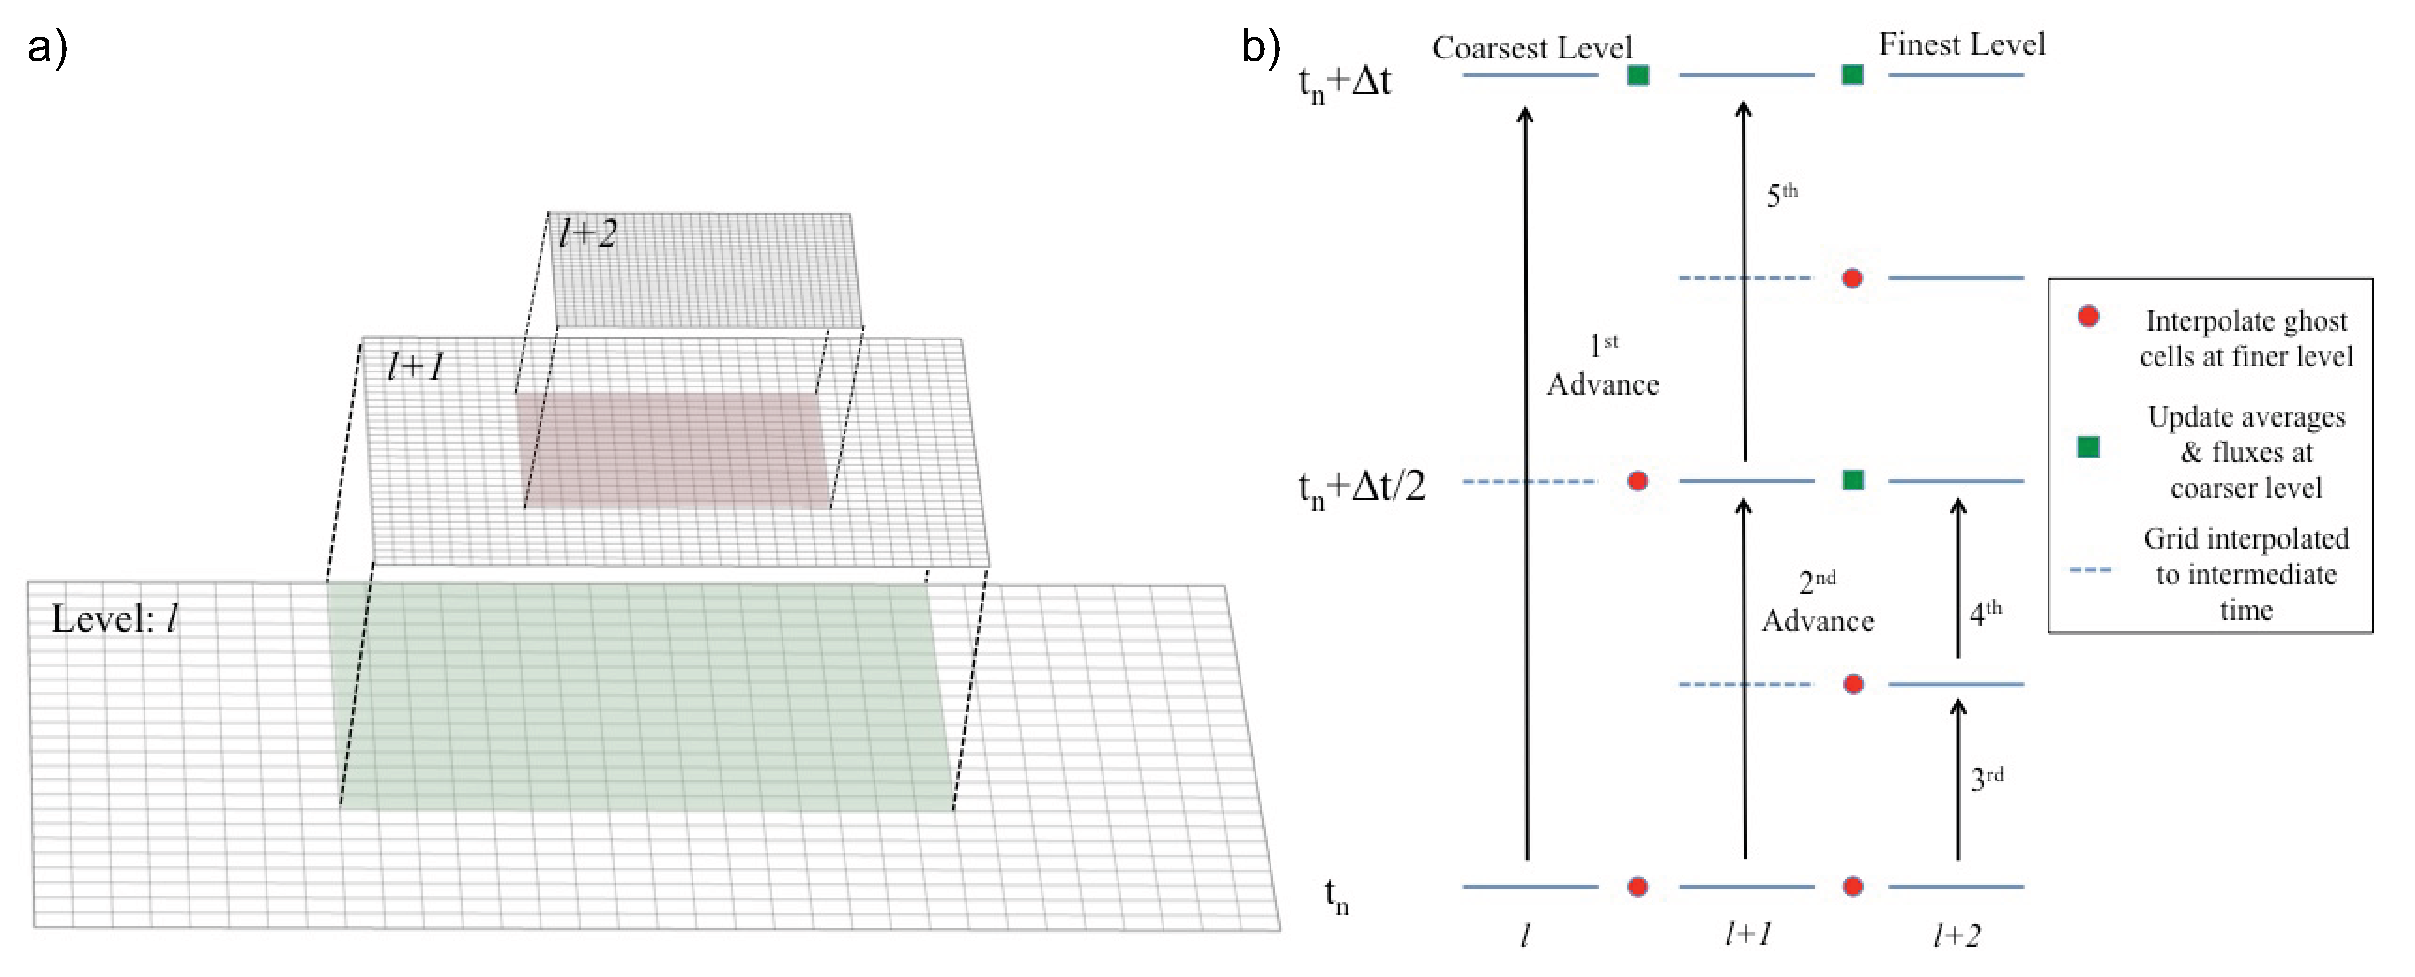
\includegraphics[width=\textwidth]{Chap1/subcyles_and_levels_h.eps}}
    \caption{(a) Example of a grid with two levels of AMR using a x2
    refinement ratio between levels.  The additional levels do not
    replace the coarse level cells underneath, they are overlaid on top.
    (b) Diagram depicting the sub-cycling of AMR levels in time.  The
    coarse level is advanced first from time $t_n$ to time $t_n +\Delta t$ where $\Delta t$ is the time step for the coarsest level. Then the finer levels are advanced
    with a smaller time step and periodic updates of fluxes from the
    coarser grids.}%
    \label{fig:cyclesnlevels}
\end{figure}

Figure~\ref{fig:cyclesnlevels}b depicts an overview of the time-stepping and 
sub-cycling process. Rather than having a uniform
time step dependent on the smallest grid-cell size, Chombo-AMR
sub-cycles the refined levels in time maintaining a constant Courant
number.  As noted by \cite{ullrich2014understand} the single-wave-mode characteristics of a numerical method often have an
unexpected and non-linear dependence on the Courant number.
Therefore, a constant Courant number helps ensure consistent dispersive
properties across the refinement levels. 
The typical work flow for advancing an AMR grid level $l$ in time is as
follows:
\begin{itemize}
    \item[1.]
        Regrid levels finer than $l$ if required:  \newline Evaluate the refinement criterion
        and mark (tag) all cells which should be included in finer levels.
        In these regions, new blocks of cells at levels $l+1$ are
        overlaid.  The new cell values are interpolated from the coarser
        level using a fourth-order least-squares algorithm that maintains
        conservation as described in Sec. 4.1 of \cite{mccorquodale2015adaptive}.
    \item[2.]
        Advance level $l$ one time step using the RK4 time-stepping
        method.
    \item[3.]
        Interpolate values to the ghost cells that surround level $l+1$
        using the least-squares algorithm also implemented for ghost cells 
        at panel boundaries. Three layers of ghost cells
        are required.  The interpolation does not need to be
        conservative as the ghost cell values are only used to
        reconstruct the flux on the faces of the level $l+1$ cells.
        Figure~\ref{fig:ghost_cells} depicts the location of ghost cells for 
        two of the three layers and the stencil of coarse grid cells used 
        for their interpolation.
    \item[4.]
        Perform previous steps for level $l+1$.  Level $l+1$ is
        advanced using refined time steps (sub-cycling) as depicted in
        Fig.~\ref{fig:cyclesnlevels}b.  A temporal interpolation closely
        related to the RK4 method is used to update the values in the 
        level $l+1$ ghost cells from cells on level $l$ at the intermediate time
        steps \citep{mccorquodale2015adaptive}.
    \item[5.]
        After the sub-cycling in time is completed, average the solution
        from level $l+1$ and sum up the fluxes to update the values on
        the coarse grid.  Corrections are applied to the fluxes at
        coarse-fine interfaces to ensure conservation \citep{berger1989local}.
\end{itemize}

\begin{figure}
    \centerline{%
    \noindent
    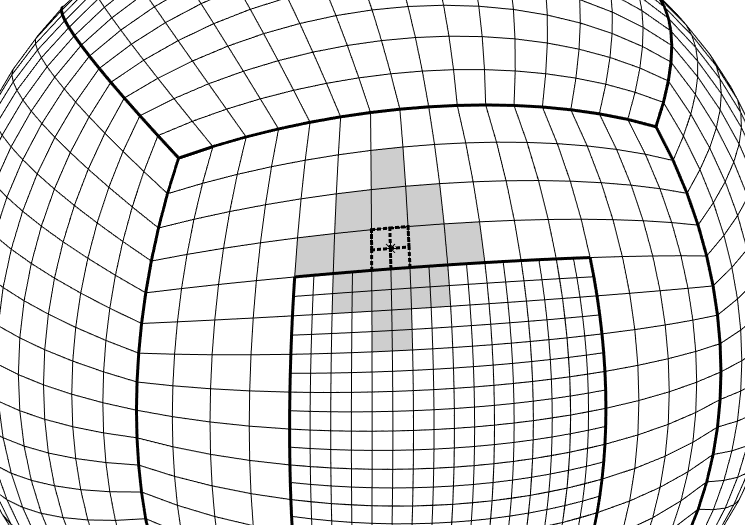
\includegraphics[width=19pc]{Chap1/cs_amr_ghostcell.png}}
    \caption{Example of a 1-level AMR approach with a refinement ratio of two
    on the cubed sphere grid.  The four dashed cells are schematic examples of ghost
    cells for the finer grid, which are interpolated from the values in
    the coarse cells shaded in gray. Our actual AMR applications need three ghost cells.}%
    \label{fig:ghost_cells}
\end{figure}

As mentioned in the description of the first step, the additional levels are placed in
locations that have been tagged by the refinement criterion of the
model.  The size of the refined grid that is added over tagged cells is
determined by three aspects: (1) the need to ensure proper nesting of finer levels,
(2) parameters from the Chombo library designed for efficient
parallelization, and (3) a user-defined buffer parameter.  Refinement (tagging)
criteria are based on thresholds for user-selected flow properties, like
relative vorticity, that indicate where refinement should be placed.
The tagging strategies can be based on a variety of properties including
tracer values, vorticity thresholds, gradients, or a combination of
several criteria.  The type of refinement criteria and the threshold
values are set independently for each simulation.  The threshold values
can be uniform across all refinement levels or designed to scale with
increasing refinement.  For example, the relative vorticity threshold can be set
so that it increases with increasing resolution. With the idealized
test cases presented in this chapter, the selection of refinement criteria
and thresholds was problem-dependent, with the simplicity of the
tests offering only a few possible options.  A range of refinement
thresholds for the AMR test cases was explored. Here, we present 
various thresholds for the gravity wave and binary vortices tests to
demonstrate how changes in refinement affect the solutions and grids.
For the moving-vortices advection test we only present a single 
threshold value that represents a compromise between reducing the
error and increasing the computational run time.

The Chombo-AMR dycore is designed to have multiple refinement levels (up
to ten), and the maximum number of levels is set for each simulation.
In our simulations, we explore the effects of adding up to
two refinement levels (called 2-level AMR).  In addition, we explore the
grid-resolution refinement ratios between successive levels,
and present selected results for three powers of two: x2, x4 and x8.
As an example, a grid with a base level of
c32 ($2.8^\circ$) resolution and 2 levels of x4 refinement has
a maximum resolution of c512 ($0.18^\circ$). 

\section{Results of the Numerical Experiments}
\label{sec:results}
For our assessment of the
Chombo-AMR shallow-water model, we select five test cases: one advection
test and four shallow-water tests.  The test cases are divided into two
categories:  large-scale smooth flows and
simulations with either sharp gradients or strong, non-linear, localized
flows.  The first category is comprised of the following two
shallow-water tests:
\begin{itemize}
    \item
        a steady-state geostrophic flow (test case 2 in
        \cite{Williamson:1992kx})
    \item
        an unsteady solid body rotation (example 3 from
        \cite{Lauter:2005uq}).
\end{itemize}
These large-scale flows, which have no realistic use for AMR, serve as
``do no harm'' tests.  They are used to check the model's ability to
preserve the characteristics of smooth flows as they cross the AMR
patches.  We measure the impact that the refinement ratios, the number
of AMR levels, and the location of the refinement patches have on the
solution.  Convergence tests are also performed with these test cases that both have analytical solutions.

The second test category with localized flow features consists of three tests for which
AMR could improve the solution, and we seek to evaluate how effectively
it is able to do so. These tests are
\begin{itemize}
    \item
        the moving vortices advection test by
        \cite{Nair:2008fk} (with analytical solution)
    \item
        a gravity wave impinging on an idealized mountain shallow-water
        test.
    \item
        a binary-vortices test case in which two vortices interact.
\end{itemize}
The bottom two do not have analytical solutions and the evaluations rely on
high-resolution reference solutions.
A variety of refinement criteria are used with these test cases to
demonstrate the AMR's ability to track, adapt to, and resolve these
localized features accurately.  The model results are presented using
normalized $l_2$ and $l_\infty$ error norms as defined in
\cite{Williamson:1992kx}.  Additionally, the total number of grid cells
quoted for AMR runs include the sum of all valid grid cells from all
refinement levels (not including ghost cells) since the finer levels
overlay the coarser grids beneath them.  The total number of grid cells
can serve as a rough benchmark of computational cost when comparing AMR
runs to uniform runs.

The model results are presented using
normalized $l_2$ and $l_\infty$ error norms as defined in
\cite{Williamson:1992kx}. These errors for computed variable field $h$ are calculated
 via the usual global error norms,
\begin{equation}
   \label{eq:l2} l_2(h) = \sqrt{\frac{I\left[(h-h_\tau)^2\right]}{I\left[h_\tau^2\right]}}
\end{equation}
\begin{equation}
   \label{eq:lmax} l_\infty(h) = \frac{\max|h-h_\tau|}{\max|h_\tau|}
\end{equation}
where $h_\tau$ is the reference field and $I$ is a discrete approximation
to the global integral given by
\begin{equation}
    \label{eq:globint} I[x] = \sum_{\text{all cells } k} x_k A_k
\end{equation}
where $A_k$ denotes the area of grid cell $k$.

\subsection{Moving-Vortices Advection Test} 
\label{subsec:moving-vortices}

The moving-vortices test is
a challenging deformational-flow advection test proposed by
\cite{Nair:2008fk}.  The test represents the roll-up of an initially
smooth tracer into tight spiral bands. The roll-up creates steep
gradients which provide a good test for the AMR.  In this test, a pair
of vortices is generated on diametrically opposite sides of the sphere.
The wind field is the summation of a solid-body rotation and a
deformational flow such that the two vortices move along a great circle 
and an exact solution is known at all times [see \cite{Nair:2008fk} for details].

A 12-day time period is simulated,
which advects the spiraling vortices once around the sphere.  The
background flow is prescribed with a rotation angle of $\alpha=\pi/4$
so that the two vortices are advected through the corners of the
cubed-sphere (located at $\pm 45^\circ$).
Figures~\ref{fig:spradverrplots}a--d depict the analytical solution for the roll-up of the tracer at
days 0, 4, 8, and 12.
%
\begin{figure}
    \centerline{%
    \noindent
    \includegraphics[width=\textwidth]{Chap1/sprl_adv_err.eps}}
    \caption{(a)--(d): Analytic tracer field at days 0, 4, 8, and 12
for the moving-vortices advection test of
Section~\ref{subsec:moving-vortices}.
    (e)--(h): Tracer error at the select days for a 2-level AMR run with a
    c32 base resolution using x4 refinement (c32/c128/c512) and the
    tracer-gradient refinement tagging criterion.  (i)--(l): same as (e)--(h)
    but with the combination of relative-vorticity magnitude and tracer-gradient
    criterion.  The adaptive block-structure is shown by black
    lines.  The thickest lines are the base c32 grid, and thinner lines
    represent the c128 and c512 levels.  Note (e)--(h) have different
    contour scale than (i)--(l).}%
    \label{fig:spradverrplots}
\end{figure}
%
Numerical tests were carried out with uniform grids and AMR grids with
two different tagging criteria:  a tracer-gradient tagging and a
combination tagging.  In tracer-gradient tagging, the model refines in
regions where $|\nabla q| > 1.5 \times 10^{-7}$ $\mathrm{m}^{-1}$,
where 
$q$ is the unitless value of the passive tracer.  Combination tagging
combines the tracer-gradient tagging criterion with a relative-vorticity
tagging that refines in areas where 
$| \zeta | > 1.45 \times 10^{-5}\mathrm { s}^{-1}$, 
so that the model refines over regions in which either
threshold is reached. 
The gradient threshold value demonstrates a balance between 
reducing error and limiting computational costs. 
A lower threshold increases run time without significantly 
reducing error and a higher one results in a large increase in error. 
The vorticity threshold is set to maximize initial refinement around 
the vorticity patches without being 
too low as to refine on the background vorticity.
With both criteria, a x4 refinement ratio between
levels was used.  The evolution of the grids can be seen in
Fig.~\ref{fig:spradverrplots}, which shows the tracer error for the two AMR
runs. 
Figures~\ref{fig:spradverrplots}e--h depict the 2-level AMR run (c32/c128/c512),
which has a base grid with c32 resolution, a c128 intermediate AMR
level, and a finest c512 AMR level, using the tracer-gradient tagging.
Figures~\ref{fig:spradverrplots}i--l depict the same 2-level AMR setup but with
the combination tagging.  The adaptive block-structure is clearly
successful at tracking the evolving vortices.  The block structure of
patches, not the individual grids cells, is outlined by the black lines
in Fig.~\ref{fig:spradverrplots}.  Each patch contains a user-selected maximum
number of grid cells.  However, patches might also be split into smaller
blocks by the Chombo library.  This optimizes the load-balancing of the
model on parallel computing architectures and increases the efficiency of
the code.  Therefore, various patch sizes are present in
Fig.~\ref{fig:spradverrplots}.
%
\begin{figure}
    \centerline{%
    \noindent
    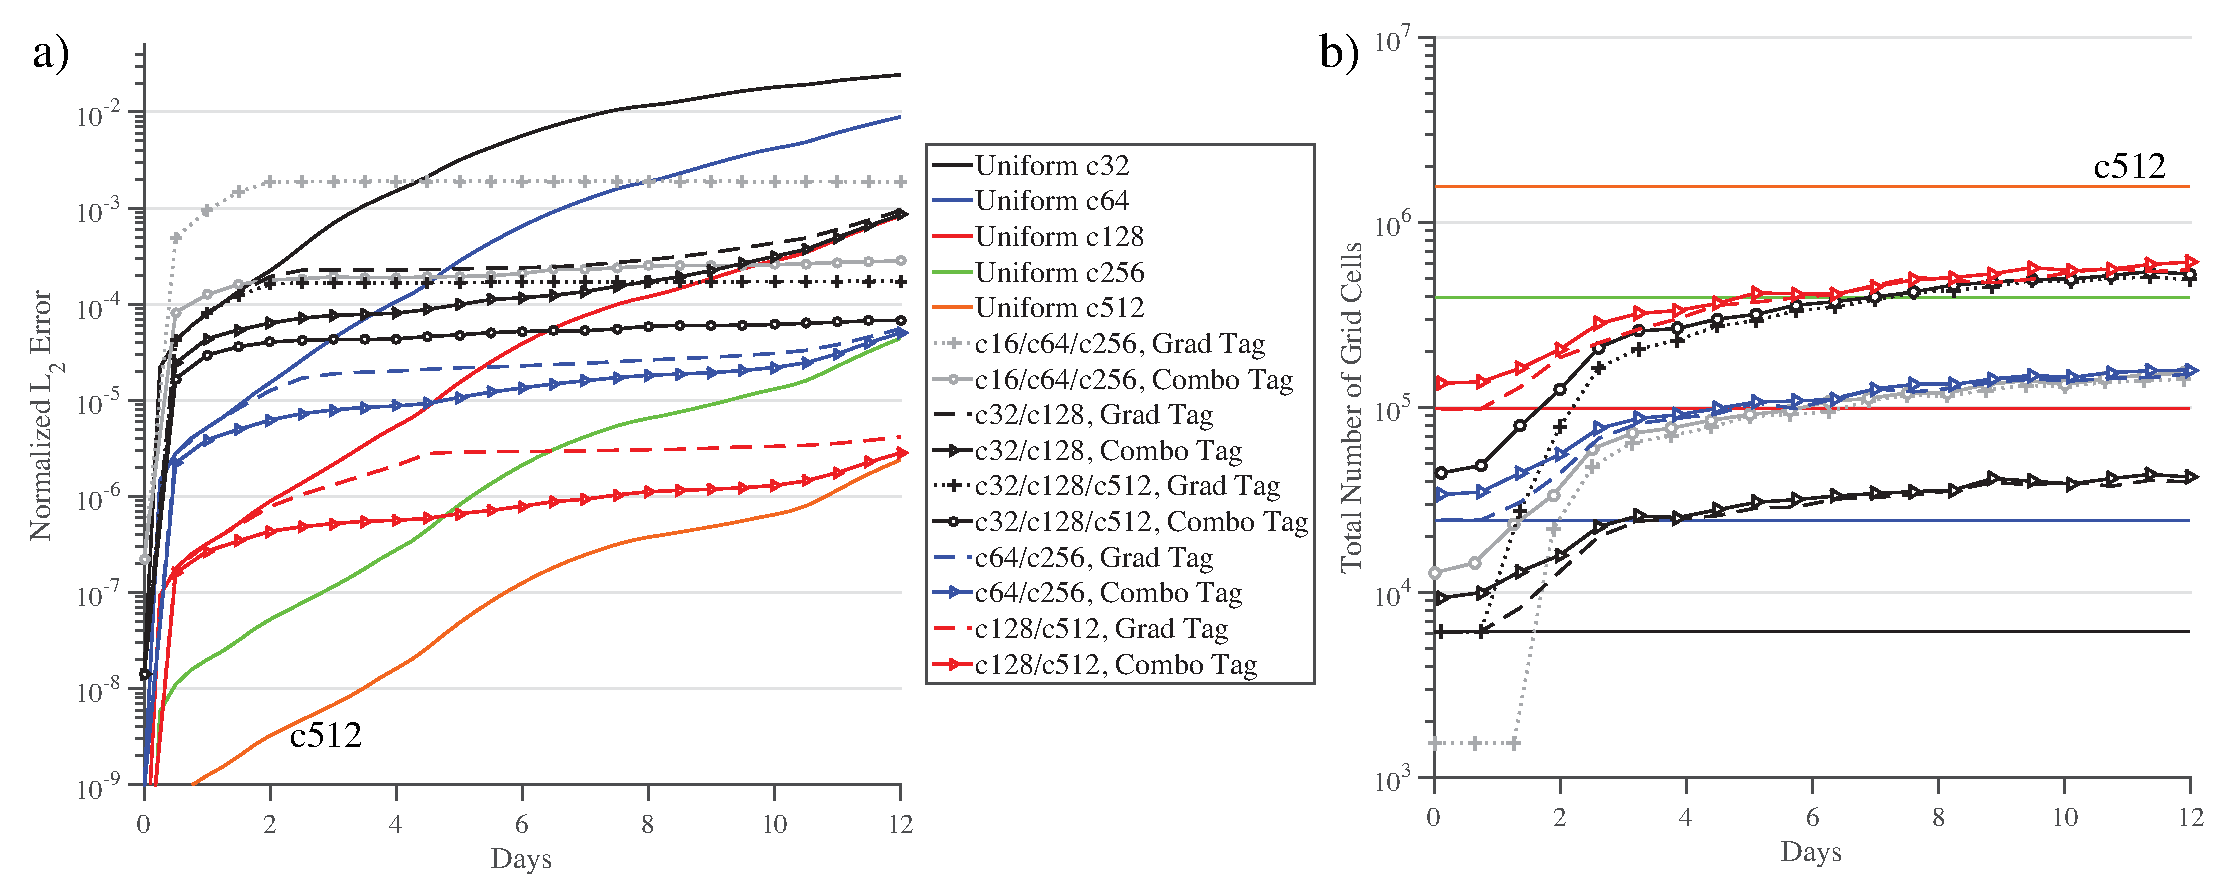
\includegraphics[width=\textwidth]{Chap1/final_sprl_adv_err_grid_plots_w16.eps}}
    \caption{
For the moving-vortices advection test of
Section~\ref{subsec:moving-vortices},
growth over time of:
(a) normalized $l_2$ tracer error, and (b)
    total number of grid cells.  The plots
    provide a comparison of uniform runs (solid lines, no markers) and
    AMR runs using gradient tagging (broken lines, with and without
    markers) and combination of relative-vorticity and tracer-gradient
    tagging (solid lines with markers).  All AMR runs use the x4
    refinement ratio between resolution levels.}%
    \label{fig:spradvl2err}
\end{figure}
%
For the tracer-gradient tagging scheme
(Figs.~\ref{fig:spradverrplots}e--h), the error is largest near the center of
the spiral. The combination tagging scheme
(Figs.~\ref{fig:spradverrplots}i--l) significantly reduces the error near the
center, and the largest error is now towards the outer edges of the
spiral just beyond the coarse-fine grid boundaries.  When using only the
tracer-gradient tagging, refinement does not begin until after day one,
so errors accumulate on the coarse grid until that time and remain
higher even after being overlaid with finer levels.  With the
combination tagging, the central region is already refined (see
Fig.~\ref{fig:spradverrplots}i), which limits the error growth.  This effect
can also be seen in
Fig.~\ref{fig:spradvl2err}a where a time series of the normalized $l_2$
tracer errors with respect to the analytic solution are depicted for 15
different model configurations.  In particular,
Fig.~\ref{fig:spradvl2err}a compares the $l_2$ tracer errors of the five
uniform-resolution simulations c32, c64, c128, c256, and c512 (see
Table~\ref{tb:grids} for the associated grid spacings) to various 1-level and
2-level AMR experiments with either the tracer-gradient or combination
tagging.  The time evolution of the associated total number of grid
cells, including the underlying coarse cells, is shown in
Fig.~\ref{fig:spradvl2err}b.  In general, the error in the combination
tagging simulations reaches the lower error values of the uniform runs
(with the same resolution as the finest AMR level) more quickly than the
tracer-gradient tagging ones, despite having a significant
difference in grid-cell count for only the first few days (see
Fig.~\ref{fig:spradvl2err}b).
The errors in all
single-level AMR runs in
Fig.~\ref{fig:spradvl2err}a using both tagging criteria converge to the error
of uniform runs at the highest resolution (e.g., the c32/c128 AMR run and
the uniform c128 run).  This result is achieved using significantly
fewer grid cells than the uniform runs.  AMR limits the normalized 
$l_2$ error growth.  AMR runs begin with global errors that are near the level 
of uniform runs with a grid resolution of their coarsest grid.
However, their global error increases at a much slower rate than that of
the uniform runs until the AMR error approaches the error level of the
matching high-resolution uniform run.  In the simulations presented here the 2-level AMR runs see a diminishing
effectiveness at decreasing the global error as the errors from the
coarse section of the grid dominate. 
%
\begin{figure}
    \centerline{%
    \noindent
    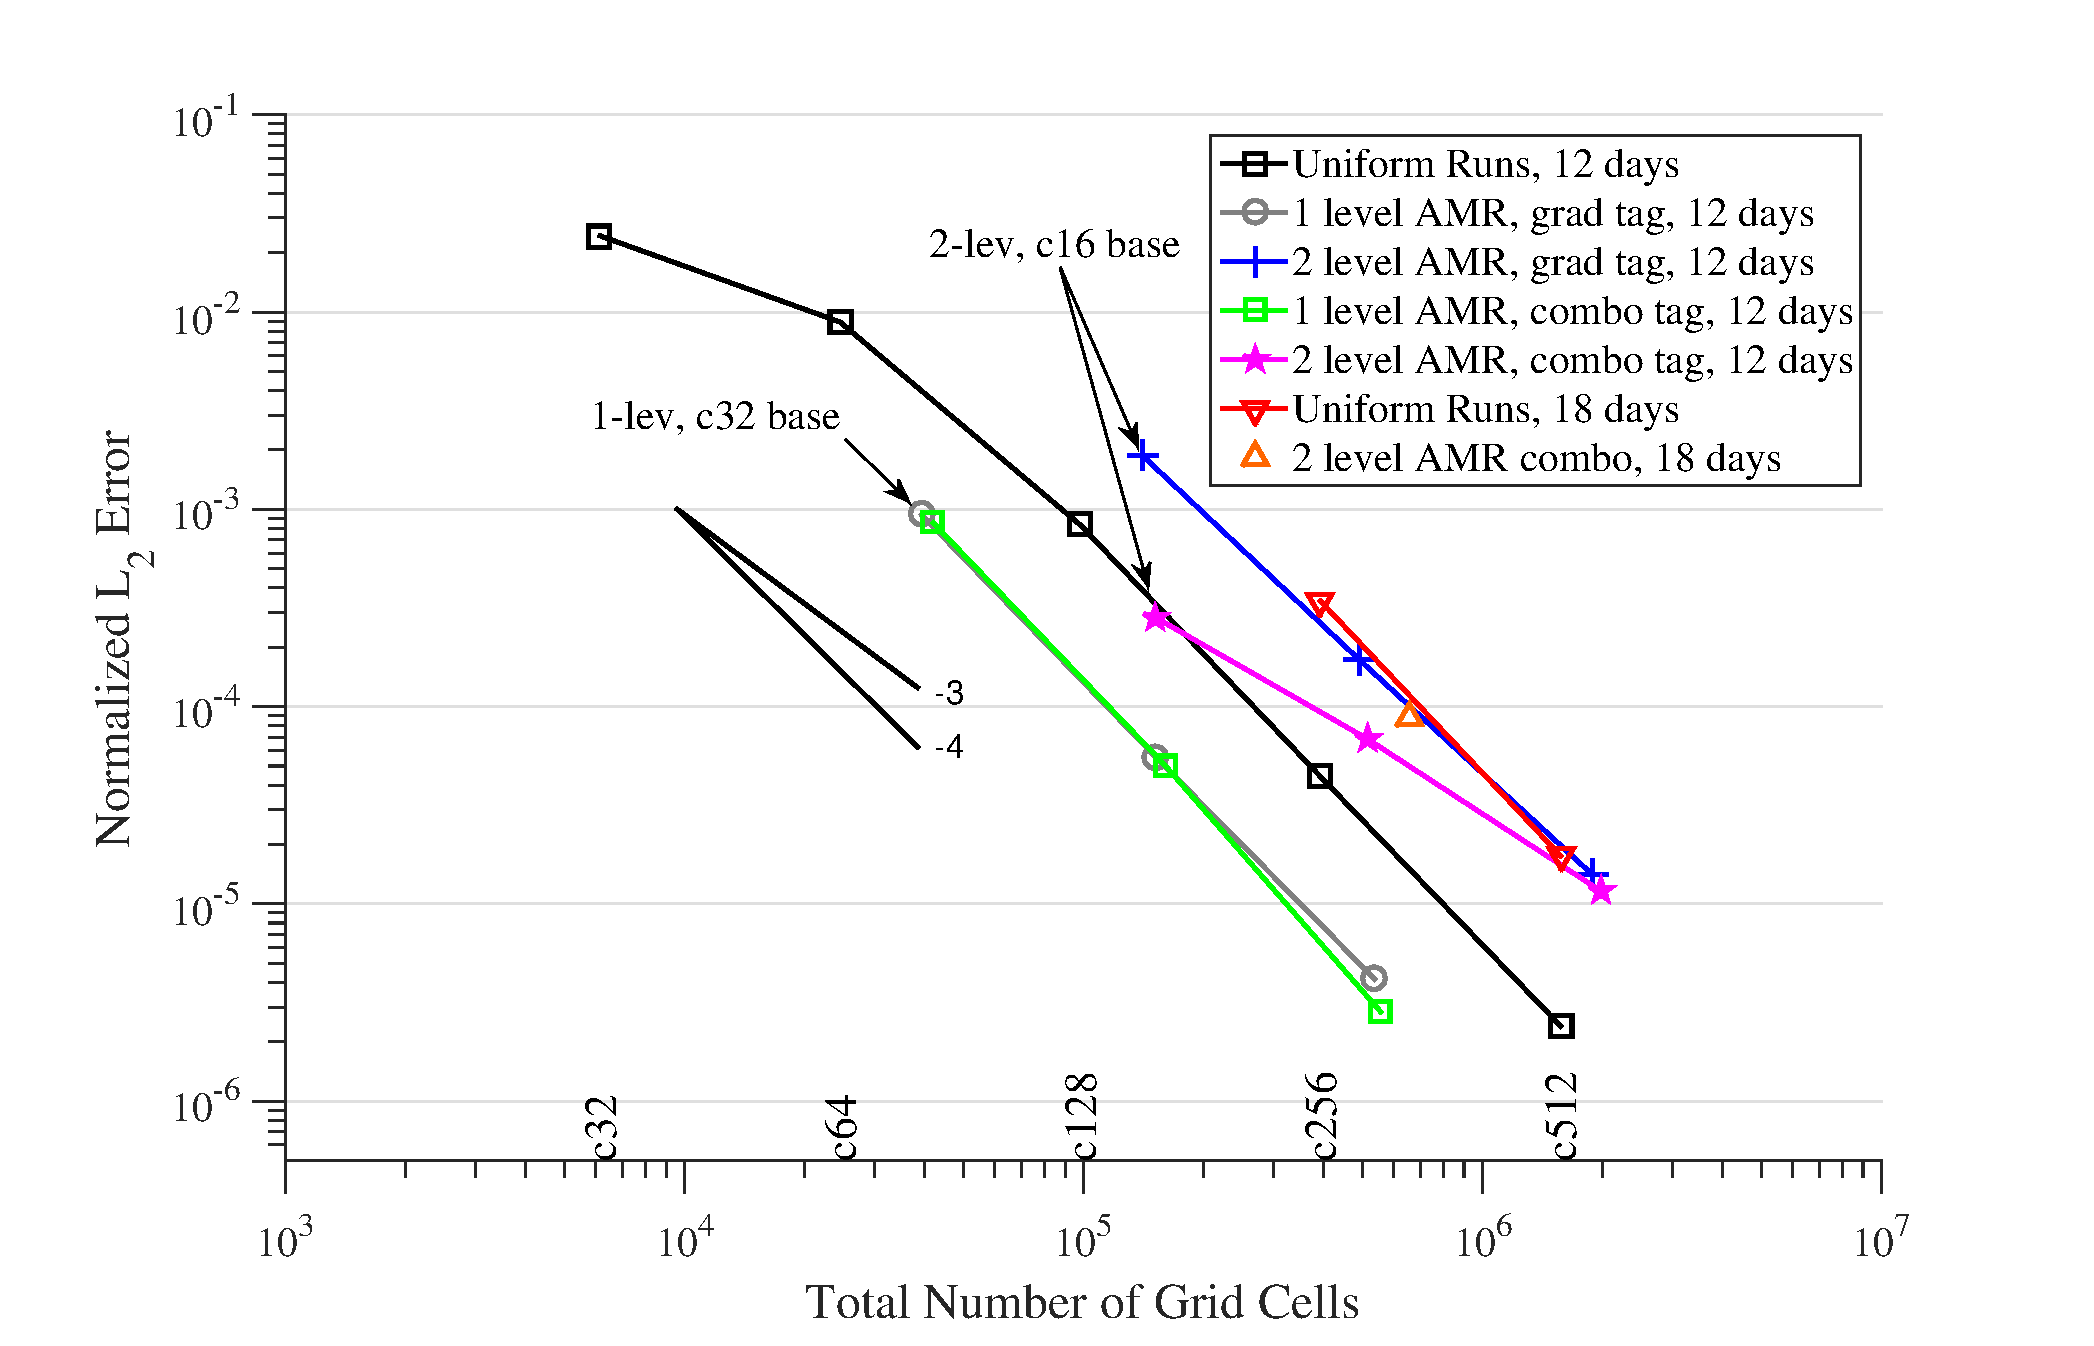
\includegraphics[width=\textwidth]{Chap1/sprladv_errvsgrid.eps}}
    \caption{Normalized $l_2$ gradient error as a function of total
    number of grid cells for the moving-vortices advection test case of
Section~\ref{subsec:moving-vortices}
 at day 12.
    The grid-resolution labels along the bottom axis note the number of
    grid cells in the uniform grids with those resolutions.  The black
    square markers are for the uniform runs c32 through c512.  The gray
    circles and green squares represent the 1-level x4 refinement AMR
    with base resolutions of c32, c64, and c128 using gradient tagging
    and combination tagging, respectively.  The blue crosses and magenta
    stars represent the 2-level x4 refinement runs with base
    resolutions of c16, c32, and c64 using gradient tagging and
    combination tagging, respectively.  Finally, the red downward-pointing
    triangles represent the uniform c256 and c512 runs at day 18, while
    the orange triangle is the 2-level x4 refinement runs with a c32
    base resolution, using the combination tagging at day 18.  Solid
    black lines depict convergence rates.}%
    \label{fig:spradvl2vgrid}
\end{figure}
%
The error at day 12 as a function of total number of grid cells for both
uniform and AMR runs is plotted in
Fig.~\ref{fig:spradvl2vgrid}.  AMR runs that have error values plotted to the
left of the errors of the uniform runs (line of hollow black squares)
achieve a lower $l_2$ error than a uniform run with a comparable
number of grid cells.  While the 1-level AMR runs show a decrease in
error while using fewer grid cells, the 2-level AMR runs generally result in a
higher error for a comparable number of grid cells than the uniform runs.  Only
the 2-level AMR run with a c16 base using the combination tagging has a
slightly improved error compared to the uniform runs (see the leftmost magenta star).  
These results demonstrate the reduced improvement to the global error from additional
levels of AMR with very coarse base meshes.  
However, AMR still slows down the error growth over time in comparison to uniform runs, and even asymptotes
to the finest uniform mesh errors (c128/c512, for example).  
Extending the run
time to 18 days, the $l_2$ error from the c32 base 2-level AMR run
with the combination tagging (orange triangle in
Fig.~\ref{fig:spradvl2vgrid}) is now slightly lower than the error from the
uniform runs at day 18 (red downward-pointing triangles).
Figure~\ref{fig:spradvl2vgrid} also confirms that the convergence rate for the
uniform run is fourth-order in the normalized $l_2$ error.

\cite{Nair:2008fk} applied this test using an $\alpha=0^\circ$ setup (not
$\alpha = 45^\circ$ as we present here) in an FV-AMR model 
using a coarse $5^\circ$ base grid and one to three levels of x2
refinement which were guided by a tracer-gradient threshold.  Their AMR errors
were generally the same or lower than the errors of their comparable uniform
runs for coarse grids with one or two levels of refinement.  However,
for their 3-level AMR run (finest resolution $0.625^\circ$) errors were
slightly higher than their uniform $0.625^\circ$ run, agreeing with what we observe for
multiple levels of AMR.  Additionally, our error measures for uniform-resolution runs are
comparable to other higher-order models.  Our uniform c64 
($\sim 1.4^\circ$) run with 
$\alpha=45^\circ$ has a normalized $l_2$ error of $8.9\times 10^{-3}$ 
after twelve days, which is comparable to the results from the 
$1.25^\circ$ grid using a multi-moment method in
\cite{chen2011multi} and slightly higher than the c80 ($1.125^\circ$) run
in
\cite{lauritzen2010conservative}.
%
\begin{table}
    \caption{Run times (wall-clock time in s and as \% of c512 run time)
for 12-day moving-vortices advection simulations
(Section~\ref{subsec:moving-vortices}).
    These runs had a maximum resolution of
    c512, performed on two nodes of NCAR's Yellowstone computing platform with 32 processors total. 
    Number of cells per refinement level is given at day 12, and
    as a percent of the c512 uniform run. }%
    \label{tb:adv_time}
    \resizebox{\textwidth}{!}{
    \begin{tabular}{rcrrrrrr}
        \hline
        Base Res.          & AMR Levels         & Run Time (s)            & Run Time (\%)            & c32 cells               & c128 cells              & c512 cells          & Total cells (\%) \\ 
        \hline
        \hline
        c512               & -                  & $24152$                 & $100\%$                  & $0$                     & $0$                     & $1.6 \times 10^{6}$ & $100\%$          \\ 
        c128               & 1                  & $10116$                 & $42\%$                   & $0$                     & $9.8 \times 10^{4}$     & $4.5 \times 10^{5}$ & $34\%$           \\ 
        c32                & 2                  & $10468$                 & $43\%$                   & $6.1 \times 10^{3}$     & $4.2 \times 10^{4}$     & $4.6 \times 10^{5}$ & $32\%$           \\ 
        \hline
        \hline
    \end{tabular}
    }
\end{table}
%
We also include the total run time versus number of grid cells in 
Table 
\ref{tb:adv_time},
for some of the 12-day runs  in
Fig.~\ref{fig:spradvl2vgrid}.
In this case, the wall-clock time (as a \% of the finest uniform run)
is closely related to the total number of grid points, because most of
the time steps and grid cells are at the finest level.
For AMR runs, coarser levels must be completed before fine levels.
There is therefore a slight performance penalty for the 2-level AMR (c32/c128/c512)
run, which actually increases the total number of finest-level points. This configuration
only has 24 boxes (each $16\times16$ cells) at the c32 level to be
distributed across 32 processors on the Yellowstone computing platform (operated 
by the National Center for Atmospheric Research (NCAR)). This means that some processors run idle when the
solution on the coarsest grid is computed which slightly lessens the parallel performance
of this AMR run.
Overall, a good heuristic for this test is that the run time is 
approximately proportional to the total number of grid cells at the
finest level.

\subsection{Global Steady-State Geostrophic Flow} 
\label{subsec:steady-state}

This zonal
steady-state flow is the second test case from the
\cite{Williamson:1992kx} test case suite for the shallow-water equations
on the sphere.  The test consists of a solid-body rotation along an axis
that differs from the polar axis by angle $\alpha$ and a corresponding
balanced height field. The steady state background velocity field in
latitude $\theta$ and longitude $\lambda$ coordinates is
\begin{equation}
    \label{eq:test2u} u = u_0\left(\cos\theta \cos\alpha +
       \cos\lambda \sin\theta\sin\alpha\right)
\end{equation}
 \begin{equation}
    \label{eq:test2v} v = -u_0 \sin\lambda \sin\alpha
\end{equation}
 where the background velocity $u_0 = \pi / 6$ Earth radii day$^{-1} = 38.61$
 m s$^{-1}$. The analytic height field is given by
\begin{equation}
    \label{eq:test2h} h = h_0 - \frac{1}{g}\left(\Omega u_0 +\frac{u_0^{2}}{2}\right)
        \left(-\cos\lambda \cos\theta \sin\alpha + \sin\theta \cos\alpha\right)^2
\end{equation}
with background height $h_0 = 2998$ m and planetary 
constants $a=6.37122 \times 10^6$ m, $\Omega = 7.292 \times 10^{-5}$ s$^{-1}$,
and $g = 9.80616$ m s$^{-2}$.

We use the more challenging $\alpha = \pi / 4$
case which means that the flow travels over the
cubed-sphere corner points at a $45^\circ$ angle.  Since the flow is
initialized in a gradient-wind balance, any changes from the initial conditions 
(which serve as the analytical solution) are considered 
errors. No topography is present. The test was designed to measure how well the model
can maintain a large-scale smooth balanced flow.  Thus, we expect little
benefit from AMR refinement.  We use the test primarily to assess the
sensitivity of the flow to the grid structure and abrupt changes in the
grid resolution along coarse-fine mesh interfaces.
%
\begin{figure}
    \centerline{%
    \noindent
    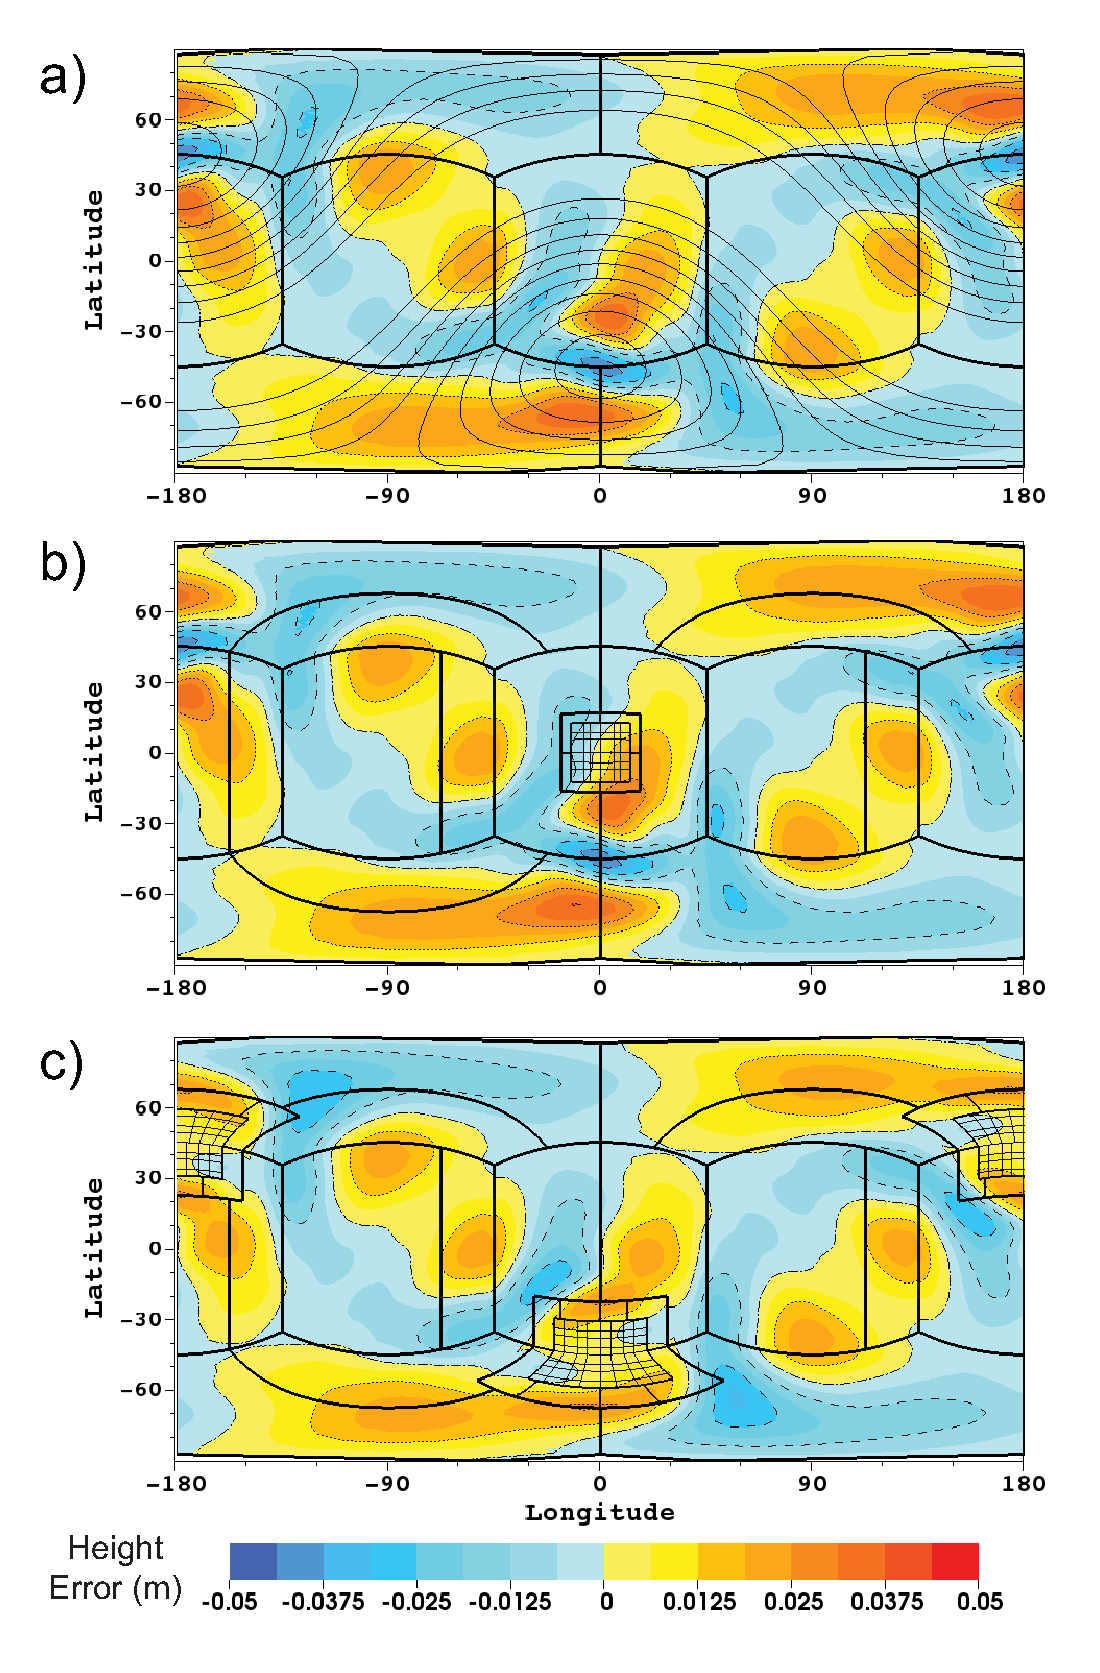
\includegraphics[width=19pc]{Chap1/test2_herrormeter_c32_day5.eps}}
    \caption{Height error (in meters) at day 5 for the steady-state
    geostrophic flow test case of
Section~\ref{subsec:steady-state}.
  The configurations are:  (a) a c32 uniform-resolution run, (b)
    a c32 grid with a static equatorial patch using two levels of x4 refinement,
    and (c) a c32 grid with static midlatitudinal patches using two levels of
    x4 refinement tagging on the relative-vorticity extrema.  The solid
    black contour lines in (a) represent the height field with a contour
    spacing of 200 m and a value range between 1200 and 2800 m with the minima encircled by the closed contours.  The
    dotted and dashed contour lines correspond to the negative and
    positive values, respectively, of the height error tick marks in the
    label bar.  The zero line is the dot-dashed line.  }%
    \label{fig:test2herrplots}
\end{figure}
%
We implement two static refinement configurations, which can be seen in
the bottom two panels of 
Fig.~\ref{fig:test2herrplots}.  The first configuration
(Fig.~\ref{fig:test2herrplots}b) consists of a statically-refined patch centered
at zero degrees latitude and longitude (fully contained within an equatorial cubed-sphere panel)
over an area with strong gradients in the height field.  In the second
configuration
(Fig.~\ref{fig:test2herrplots}c), we place static patches over the locations
of high relative vorticity, refining where 
$| \zeta | > 1.18 \times 10^{-5} \textrm{ s}^{-1}$.  
This criterion results in two midlatitudinal
patches that transect polar-equatorial panel boundaries, a challenging
location for the cubed-sphere grid.  Using these static refinement
configurations, we ran simulations that have one and two levels of
refinement using x2, x4, and x8 refinement ratios.  Increasing the
refinement ratio permits us to test how abruptly resolution can increase
without harming accuracy or causing spurious numerical noise at the
boundary between the coarse and fine regions.  We compare the height
errors, characterized as the difference between the analytic initial
condition and the numerical solution for the height at day 5, of uniform
resolution simulations and simulations using the equatorial and
midlatitudinal patch configurations.  The addition of refined patches
should ideally result in no additional error if the flow is well
resolved, or a small decrease in global height error if it is not.
%
\begin{table}[p]
    \caption{Global steady-state geostrophic flow test of
Section~\ref{subsec:steady-state}:
  Normalized $l_2$ and $l_{\infty}$ height errors at day 5 for a
    variety of refinement ratios and numbers of levels with the two
    refinement locations near the equator and in the midlatitudes.  As a comparison, the normalized height errors of a 
    uniform-resolution c32 run at day 5 are $l_2=5.4752 \times 10^{-6}$
    and $l_\infty=1.4505 \times 10^{-5}$.}%
    \label{tb:test2c32err}
    \begin{center}
    \resizebox{\textwidth}{!}{
    \begin{tabular}{cc |rr| rr}
             %
            \multicolumn{2}{c|}{} & \multicolumn{2}{c|}{Equatorial Refinement} & \multicolumn{2}{c}{Midlatitudinal Refinement} \\ 
            AMR Levels         & Ref. Ratio         & $l_2$ error             & $l_{\infty}$ error       & $l_2$ error             & $l_\infty$ error        \\ 
            \hline
            \hline
            1                  & x2                  & $5.4848 \times 10^{-6}$ & $1.4519 \times 10^{-5}$  & $4.7472 \times 10^{-6}$ & $1.0077 \times 10^{-5}$ \\ 
            1                  & x4                  & $5.4837 \times 10^{-6}$ & $1.4542 \times 10^{-5}$  & $4.7835 \times 10^{-6}$ & $9.5043 \times 10^{-6}$ \\ 
            1                  & x8                  & $5.4875 \times 10^{-6}$ & $1.4592 \times 10^{-5} $ & $4.8233 \times 10^{-6}$ & $9.6988 \times 10^{-6}$ \\ 
            2                  & x2                  & $5.4849 \times 10^{-6}$ & $1.4520 \times 10^{-5}$  & $4.5341 \times 10^{-6}$ & $1.0559 \times 10^{-5}$ \\ 
            2                  & x4                  & $5.4836 \times 10^{-6}$ & $1.4542 \times 10^{-5}$  & $4.7983 \times 10^{-6}$ & $1.1019 \times 10^{-5}$ \\ 
            \hline
        \end{tabular}
        }
    \end{center}
\end{table}
%
Results in
Table~\ref{tb:test2c32err} show the normalized $l_2$ and $l_\infty$ height
errors for the uniform c32 ($2.8^\circ$) run and c32 base runs with
the two refinement configurations after five days. The errors for the runs with the
equatorial patch are essentially unchanged from that of the uniform c32
run.  Even the extreme cases of a x8 refinement ratio or multiple levels
of refinement increase the $l_2$ height error by less than $0.25\%$.
The results for midlatitudinal patch runs show a reduction in global
error with even a x8 refinement ratio reducing the $l_2$ height error
by more than $10\%$ and the $l_\infty$ error by at least $25\%$
compared to the c32 uniform run.  The height error plots at day 5 for
the uniform c32 run and the runs for the two refinement configuration
using two levels of x4 additional refinement
(Fig.~\ref{fig:test2herrplots}a-c) depict a similar result.  The equatorial
patch run
(Fig.~\ref{fig:test2herrplots}b) has essentially the same height error profile
as the uniform run
(Fig.~\ref{fig:test2herrplots}a).  The height error for a base c32 run with
the midlatitudinal refinement patches
(Fig.~\ref{fig:test2herrplots}c) shows a clear improvement in error since the
coarse base resolution does not fully resolve the flow and the refined
patches cover areas of high error.  The refined patches do not create
any spurious wave reflections or lead to an increase in error along the
coarse-fine boundary.
%
\begin{figure}
    \centerline{%
    \noindent
    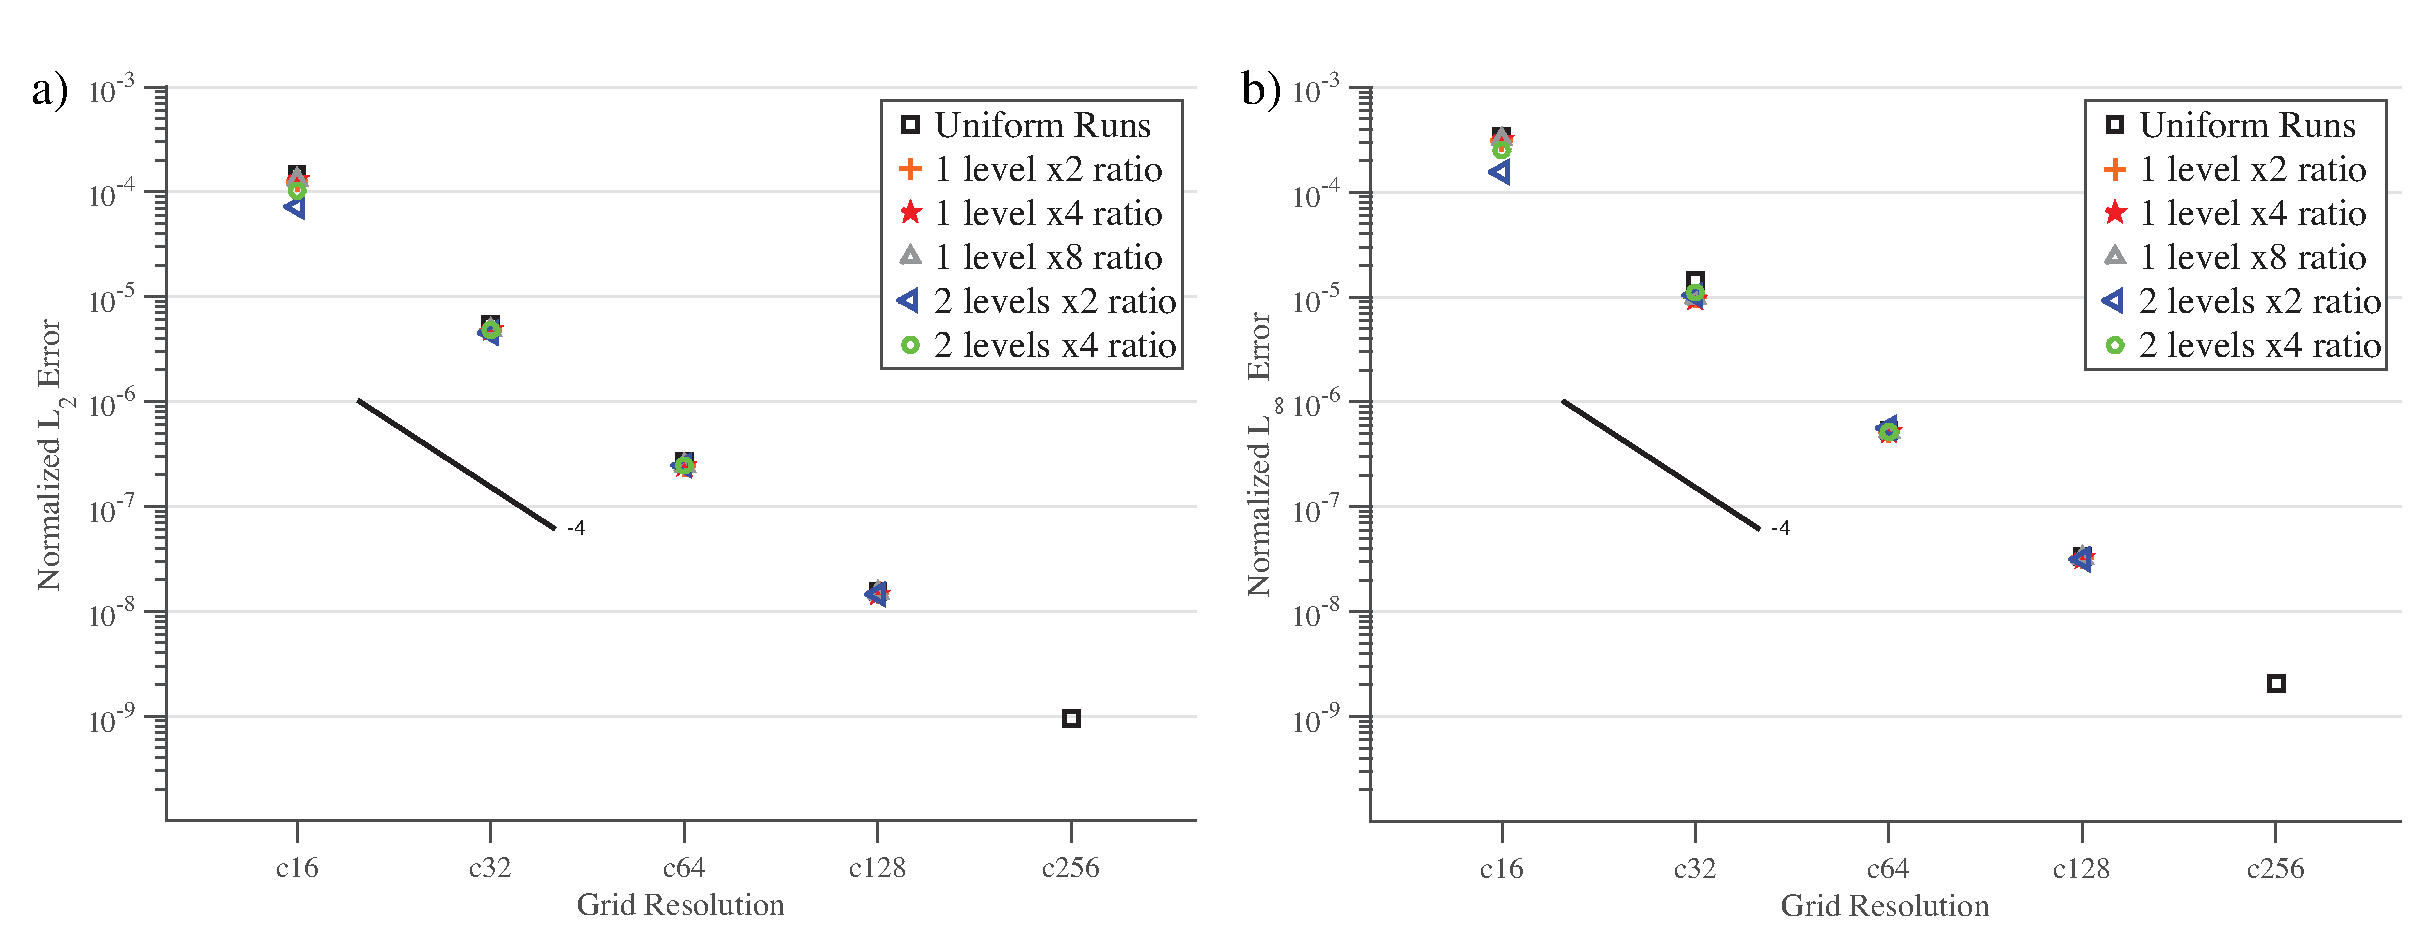
\includegraphics[width=\textwidth]{Chap1/final_Test2_errvsgrids_combo.eps}}
    \caption{(a) Normalized $l_2$ and (b) $l_\infty$ height errors
    at day 5 as a function of base grid resolution for the steady-state
    geostrophic flow test case of
Section~\ref{subsec:steady-state}.
  Uniform runs and runs using the static
    midlatitudinal refinement patches are depicted with x2, x4, or x8
    refinement ratios.  The fourth-order convergence rate is shown by
    the black line.}%
    \label{fig:test2convergeplots}
\end{figure}
%
Figure~\ref{fig:test2convergeplots} depicts a comparison of the day-5 normalized 
$l_2$ and $l_\infty$ height errors for runs with the midlatitudinal
refinement patches and uniform runs for base resolutions of c16 (
$5.6^\circ$) to c256 ($0.35^\circ$). At coarse resolutions, we see a slight
improvement in the error for runs with refinement compared to the
uniform runs. However, at higher resolutions when the flow is well resolved
the change in error is indistinguishable.  The figure also shows that
fourth-order convergence is maintained in the runs with the static
refinement patches.  Results for runs with the equatorial refinement
patch at other higher resolutions followed a similar pattern as the c32
base runs in
Table~\ref{tb:test2c32err} and also demonstrated fourth-order convergence (not shown).

The steady-state geostrophic flow test case has been used in other AMR
and static refinement studies.  Similar refined grid locations were used
with the finite-volume AMR models in
\cite{Chen:2011kk} (on the cubed-sphere) and
\cite{st2007comparison} (on a latitude-longitude grid).  In both models, the introduction of refined
patches led to increases in error when compared with the uniform runs,
with significantly larger increases in the height error for
configurations in which the refinement patch was placed over 
strong height gradients.  The error increased by $\sim 35\%$ in
\cite{Chen:2011kk} and a factor of 2.5 in
\cite{st2007comparison}.  However, for the higher-order spectral-element
method (SEM) in
\cite{st2007comparison}, the error was considerably reduced with
the addition of a refined patch.
\cite{Weller:2009gl} tested a number of grid geometries with variable
resolutions using a x2 refinement ratio and found increases in error
when a refinement patch was added.
\cite{Harris:2013nt} used a nested-grid FV model with a x3 refinement
ratio. After five days their $l_2$ height errors roughly doubled in 
comparison to their uniform run, though their $l_\infty$ errors were nearly unchanged.
Our results with static refinements are very competitive as they show
almost no increase in error or even in some cases an improvement in the
error.  Thus, our model preserves the
large-scale flow and limits the errors at the refinement patches very effectively.

\subsection{Unsteady Solid-Body Rotation}
\label{subsec:usbr}

The time-dependent zonal flow test proposed in
\cite{Lauter:2005uq} (example 3) consists of an unsteady solid-body rotation (USBR) which is
forced by topography. It possesses an analytical solution.  The large-scale flow and
the topography are smooth, zonally symmetric and somewhat artificial.  
In particular, the topography is zero at the equator and rises to its maximum (around 11 km) at both poles.
As with the previous test case, we
expect little benefit from AMR given the smooth characteristics.  The
benefit of the USBR test is that it has the added complication of moving
features that can be tracked with AMR while still having an analytic
solution to determine the error. One can observe how well the flow is
maintained and whether numerical artifacts, if any, are created by the
resolution change at grid boundaries and by the AMR regridding process.

Using the setup described in \cite{Lauter:2005uq}, the unsteady analytic solution
can be written in latitude-longitude $(\theta, \lambda)$ coordinates as
\begin{align}
    \label{eq:usbru} u  = & u_0 \left(\sin\alpha \sin\theta \left(\cos\lambda \cos\Omega t -
         \sin\lambda \sin\Omega t\right) + \cos\alpha \cos\theta\right) \\
    \label{eq:usbrv} v  = & -u_0 \sin\alpha \left(\sin\lambda \cos\Omega t +
       \cos\lambda \sin\Omega t\right) \\
    \begin{split} \label{eq:usbrh} h = & -\frac{1}{2g}[u_0\left(\sin\alpha \cos\theta 
        \left(-\cos\lambda \cos\Omega t + \sin\lambda \sin\Omega t\right)  +
        \cos\alpha \sin\theta\right)  \\ 
        &+ a\Omega\sin\theta]^2 + \frac{1}{2g} \left(a\Omega\sin\theta\right)^2 + k_1 
     \end{split} \\
    \label{eq:usbrb} h_b = & \frac{1}{2g}\left(a\Omega\sin\theta\right)^2 + k_2
\end{align}
The solutions for the zonal $u$ and meridional $v$ velocities are dependent on time 
$t$, Earth's angular velocity $\Omega$, the velocity constant $u_0 = 2\pi a / 12$ m day$^{-1} = 38.61$ m s$^{-1}$, 
and the the solid body axis of rotation angle $\alpha$. The height field $h$ is also
dependent on the Earth radius $a =6.37122 \times 10^{6}$ m 
and constant $k_1 = 1.362 \times 10^4$ m. The surface 
topography $h_b$ has the constant offset $k_2$ which is set to zero for these simulations.
We have set the parameter $\alpha = \pi/4$ to
let the flow field pass over the corners of the cubed sphere at a 45$^\circ$ angle.  To force
the initial condition to repeat itself after exactly one day for better
comparison of the results, the Earth's angular velocity is slightly
modified to be based on a solar day instead of sidereal day, so that the
angular velocity is $\Omega = 2 \pi/86400$ s$^{-1}$ $\approx 7.2722\cdot 10^{-5}$ s$^{-1}$.

We conduct a series of simulations over a range of base resolutions with
either one or two levels of refinement using three refinement
configurations:
\begin{itemize}
    \item[1.]
        Statically refined patch used in Sec.  3b
        now centered at $0^\circ\textrm{N}$, $90^\circ\textrm{E}$.
    \item[2.]
        Dynamic AMR refinement with height tag, the threshold for the free surface height is $h > 1.38 \times 10^{4}$ m.
    \item[3.]
        Dynamic AMR refinement with relative vorticity tag, 
        the threshold is $| \zeta | > 1.18 \times 10^{-5} \textrm{ s}^{-1}$.
\end{itemize}
The three grid configurations can be seen in 
Figs.~\ref{fig:usbrherrplots}b-d, which show the patches at the identical
initial and final (day 5) positions. The second and third configurations (Figs.~\ref{fig:usbrherrplots}c,d)
provide for the AMR tracking of a moving feature, so the effects of
a moving mesh and regridding can be observed.  The vorticity tag
provides a more challenging test since it bisects a cubed-sphere panel
edge.  We see little deviation in error among the x2, x4, and x8
refinement ratio simulations, so we only discuss runs with the x4
refinement ratio. Whenever the dynamic AMR grids are moved, the underlying
topography is reinitialized with the analytical formulation given in \cite{Lauter:2005uq}.
%
\begin{table}[p]
    \caption{Day 5 normalized $l_2$ and $l_{\infty}$ height error
    norms for the unsteady solid body rotation test of
Section~\ref{subsec:usbr}.
  The c32 uniform-resolution run is compared to the static refinement runs and AMR
    runs tagging on relative vorticity and height with one and
    two refinement levels using the x4 refinement ratio.}%
    \label{tb:usbr_err}
    \begin{center}
    \resizebox{\textwidth}{!}{
    \begin{tabular}{ccll}
            \hline
            Grid Config.       & No. of levels      & $l_2$ error             & $l_\infty$ error         \\ 
            \hline
            \hline
            Uniform            & -                  & $2.6052 \times 10^{-6}$ & $7.8216 \times 10^{-6}$  \\ 
            Static             & 1                  & $2.6064 \times 10^{-6}$ & $ 8.1955 \times 10^{-6}$ \\ 
            Static             & 2                  & $2.6064 \times 10^{-6}$ & $8.1977 \times 10^{-6}$  \\ 
            AMR, Vorticity     & 1                  & $2.1034 \times 10^{-6}$ & $6.1509 \times 10^{-6}$  \\ 
            AMR, Vorticity     & 2                  & $2.0017 \times 10^{-6}$ & $6.8035 \times 10^{-6}$  \\ 
            AMR, Height   & 1                  & $2.8837 \times 10^{-6}$ & $8.7651 \times 10^{-6}$  \\ 
            AMR, Height   & 2                  & $2.9205 \times 10^{-6}$ & $1.0255 \times 10^{-5}$  \\ 
            \hline
            \hline
        \end{tabular}
        }
    \end{center}
\end{table}
%
Simulations were run for five days.  The normalized global $l_2$ and 
$l_\infty$ height errors after five days are shown for simulations with
a c32 base grid in
Table~\ref{tb:usbr_err}.  Errors are calculated by comparing runs to the
analytic solution of the test case.  The uniform grid results are
compared with 1- and 2-level refinement runs using the three grid
configurations.  For the static refinement simulations, the $l_2$
height error increases by approximately $0.75\%$ in comparison to the
uniform c32 run.  In the 2-level height-tag AMR run, we observe that the
$l_2$ height error increases by about $12\%$, while the 2-level
vorticity-tag AMR run decreases the error by roughly $23\%$.
Figure~\ref{fig:usbrherrplots} depicts the USBR height errors at day 5 for the
c32 uniform run and c32 base grid runs with the three grid
configurations.  For the static equatorial patch run
(Fig.~\ref{fig:usbrherrplots}b), the height errors remain nearly the same as
for the uniform run
(Fig.~\ref{fig:usbrherrplots}a), with only very slight increases in the large
error areas on the polar panels.  Along the coarse-fine boundary, no
spurious grid-induced error is observed.  In 
the height-tag AMR run (Fig.~\ref{fig:usbrherrplots}c) the errors along the
polar-equatorial panel boundaries increase, while in the vorticity-tag
AMR run
(Fig.~\ref{fig:usbrherrplots}d), we observe that the large errors on the polar
panels are reduced due to the addition of refinement over that area.
With the height-tagging, we do not see a similar improvement because the
refined patches are over the low error areas on the equatorial panel.
%
\begin{figure}
    \centerline{%
    \noindent
    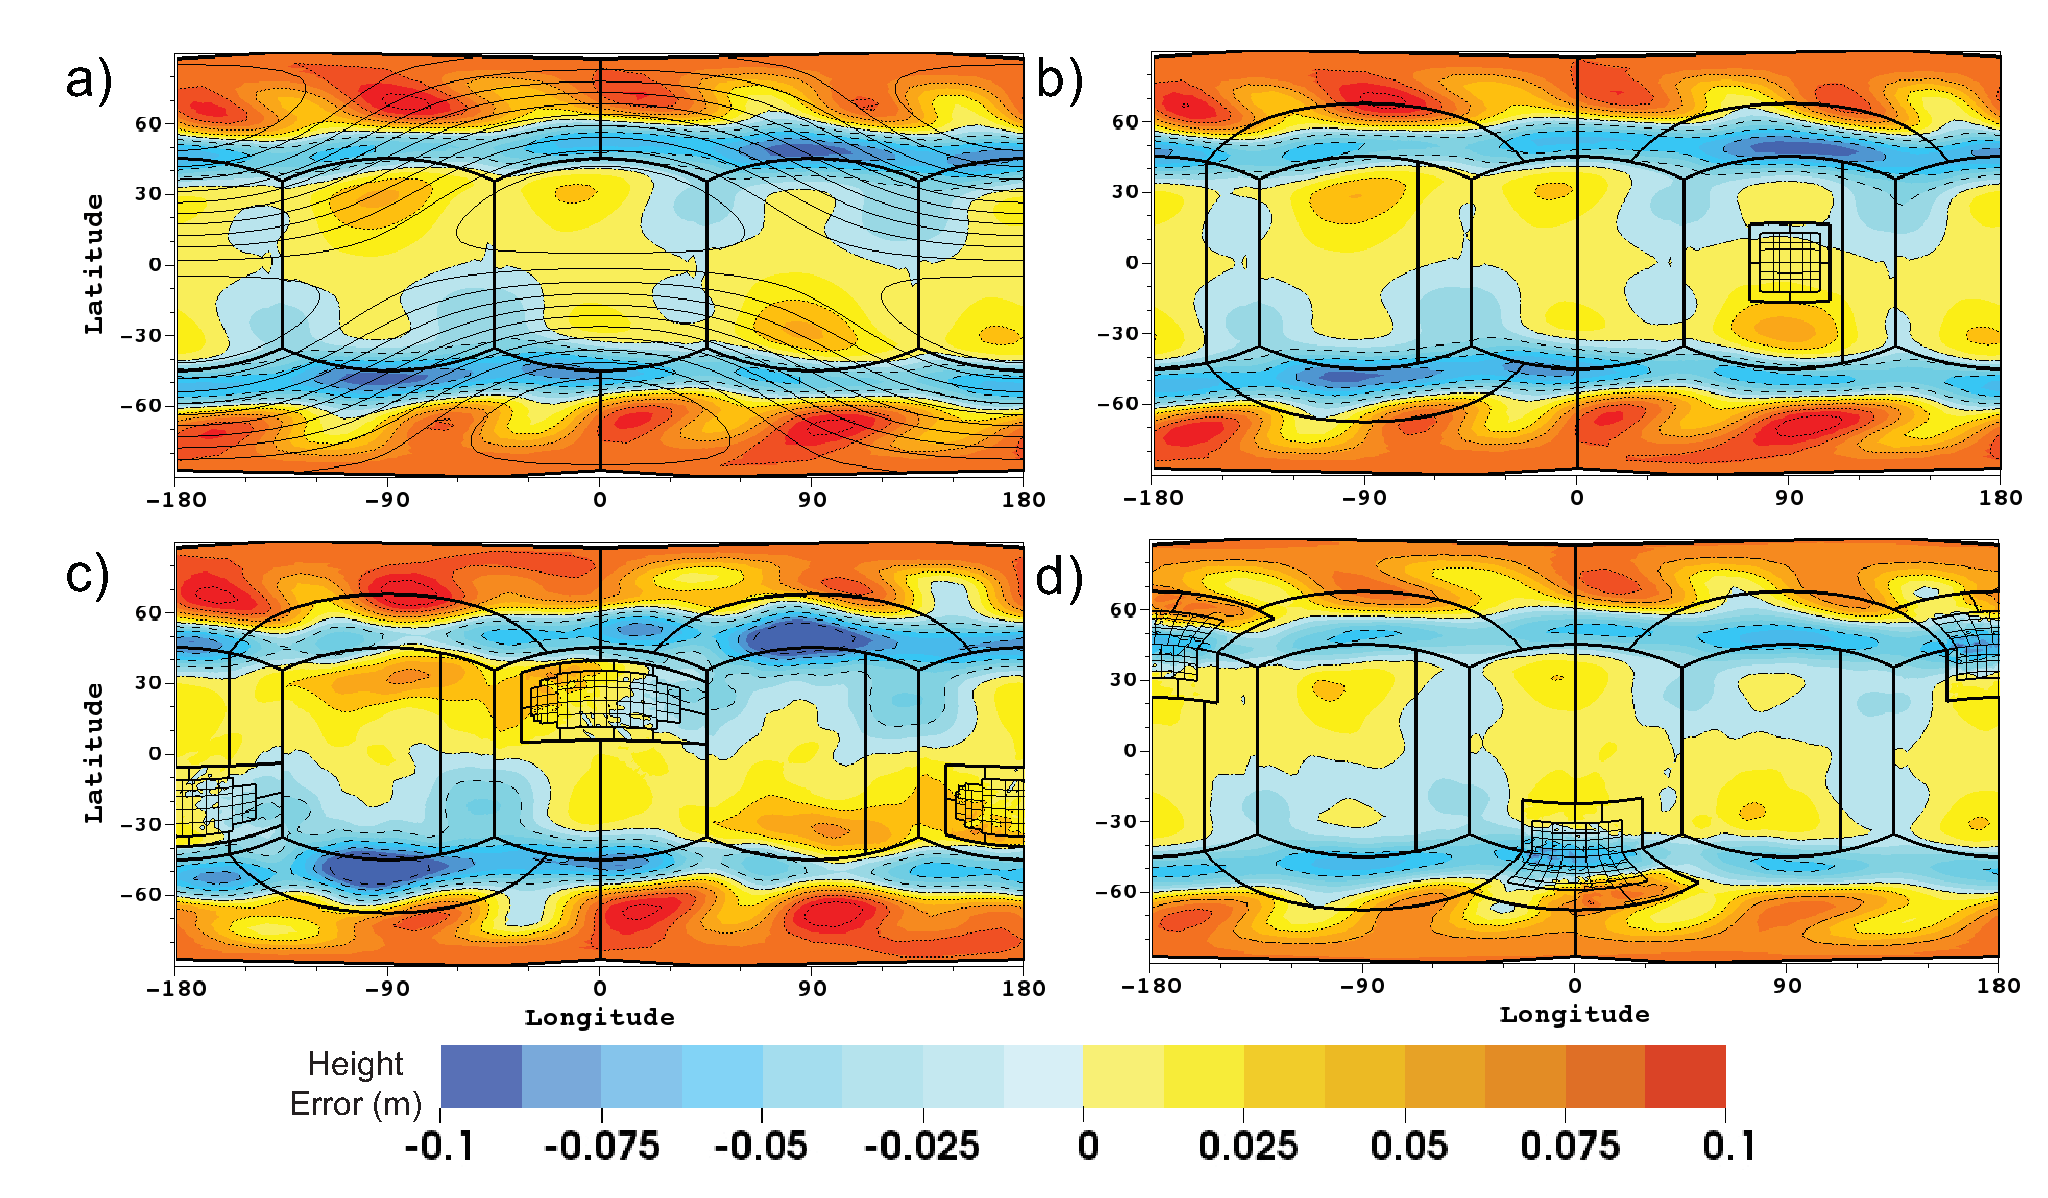
\includegraphics[width=\textwidth]{Chap1/usbr_c32_herr.eps}}
    \caption{Height field errors (in meters) at day 5 for four
simulations of the unsteady solid-body rotation test case of
Section~\ref{subsec:usbr}:
    (a) a c32 uniform-resolution run, (b) a c32 base grid with a
    static equatorial patch using two levels of x4 refinement, (c) a c32
    base grid with two levels of dynamic x4 refinement using the
    height-tag criterion, and (d) a c32 base grid with two levels of
    dynamic x4 refinement tagging on the vorticity-tag criterion.  The
    solid black contour lines in (a) represent the free surface height field of the USBR
    test (above sea level) with a 150 m contour spacing and a value range between
    $1.22\times 10^{4}$ and $1.37\times 10^{4}$ m with the minima in the polar regions.  
    The dotted and dashed contour
    lines correspond to the negative and positive values, respectively,
    of the height error tick marks in the label bar.  The zero line is
    the dot-dashed line.  }%
    \label{fig:usbrherrplots}
\end{figure}
%
After 5 days, the uniform c32 run ($\sim 313$ km grid) had a
normalized $l_2$ height error of $2.6 \times 10^{-6}$.  For
comparison, the second-order icosahedral model by
\cite{duben2012discontinuous} obtained a normalized $l_2$ height error of 
$1.05 \times 10^{-4}$ at day 5 using a uniform grid with an average edge
length of 240 km.  Other investigations focused on results at 12 hrs,
after which the flow features have progressed only half way around the
sphere.
\cite{pudykiewicz2011numerical} showed a normalized $l_2$ height error
of $\sim 6 \times 10^{-6}$ after 12 hours using a second-order
icosahedral geodesic model with a $2^\circ$ ($\sim 220$ km) grid resolution, while our
uniform c32 ($2.8^\circ$) run produced a normalized $l_2$ height error of 
$3.5 \times 10^{-7}$ at 12 hrs.  These results are comparable with those obtained by
the fourth-order multi-moment model on a Yin-Yang grid with an effective
resolution of $1.875^\circ$ in
\cite{li2015high}. They reported a normalized $l_2$ height error of $\sim 3 \times 10^{-7}$ after 12 hours. Additionally,
the third-order multi-moment method on a cubed-sphere grid with a
N=40 ($2.25^\circ$) grid resolution in
\cite{chen2014global} had a normalized $l_2$ height error of 
$\sim 6.5\times 10^{-7}$ at 12 hrs.  
We are unaware of other results that use the USBR test with AMR
applications.
%
\begin{figure}
    \centerline{%
    \noindent
    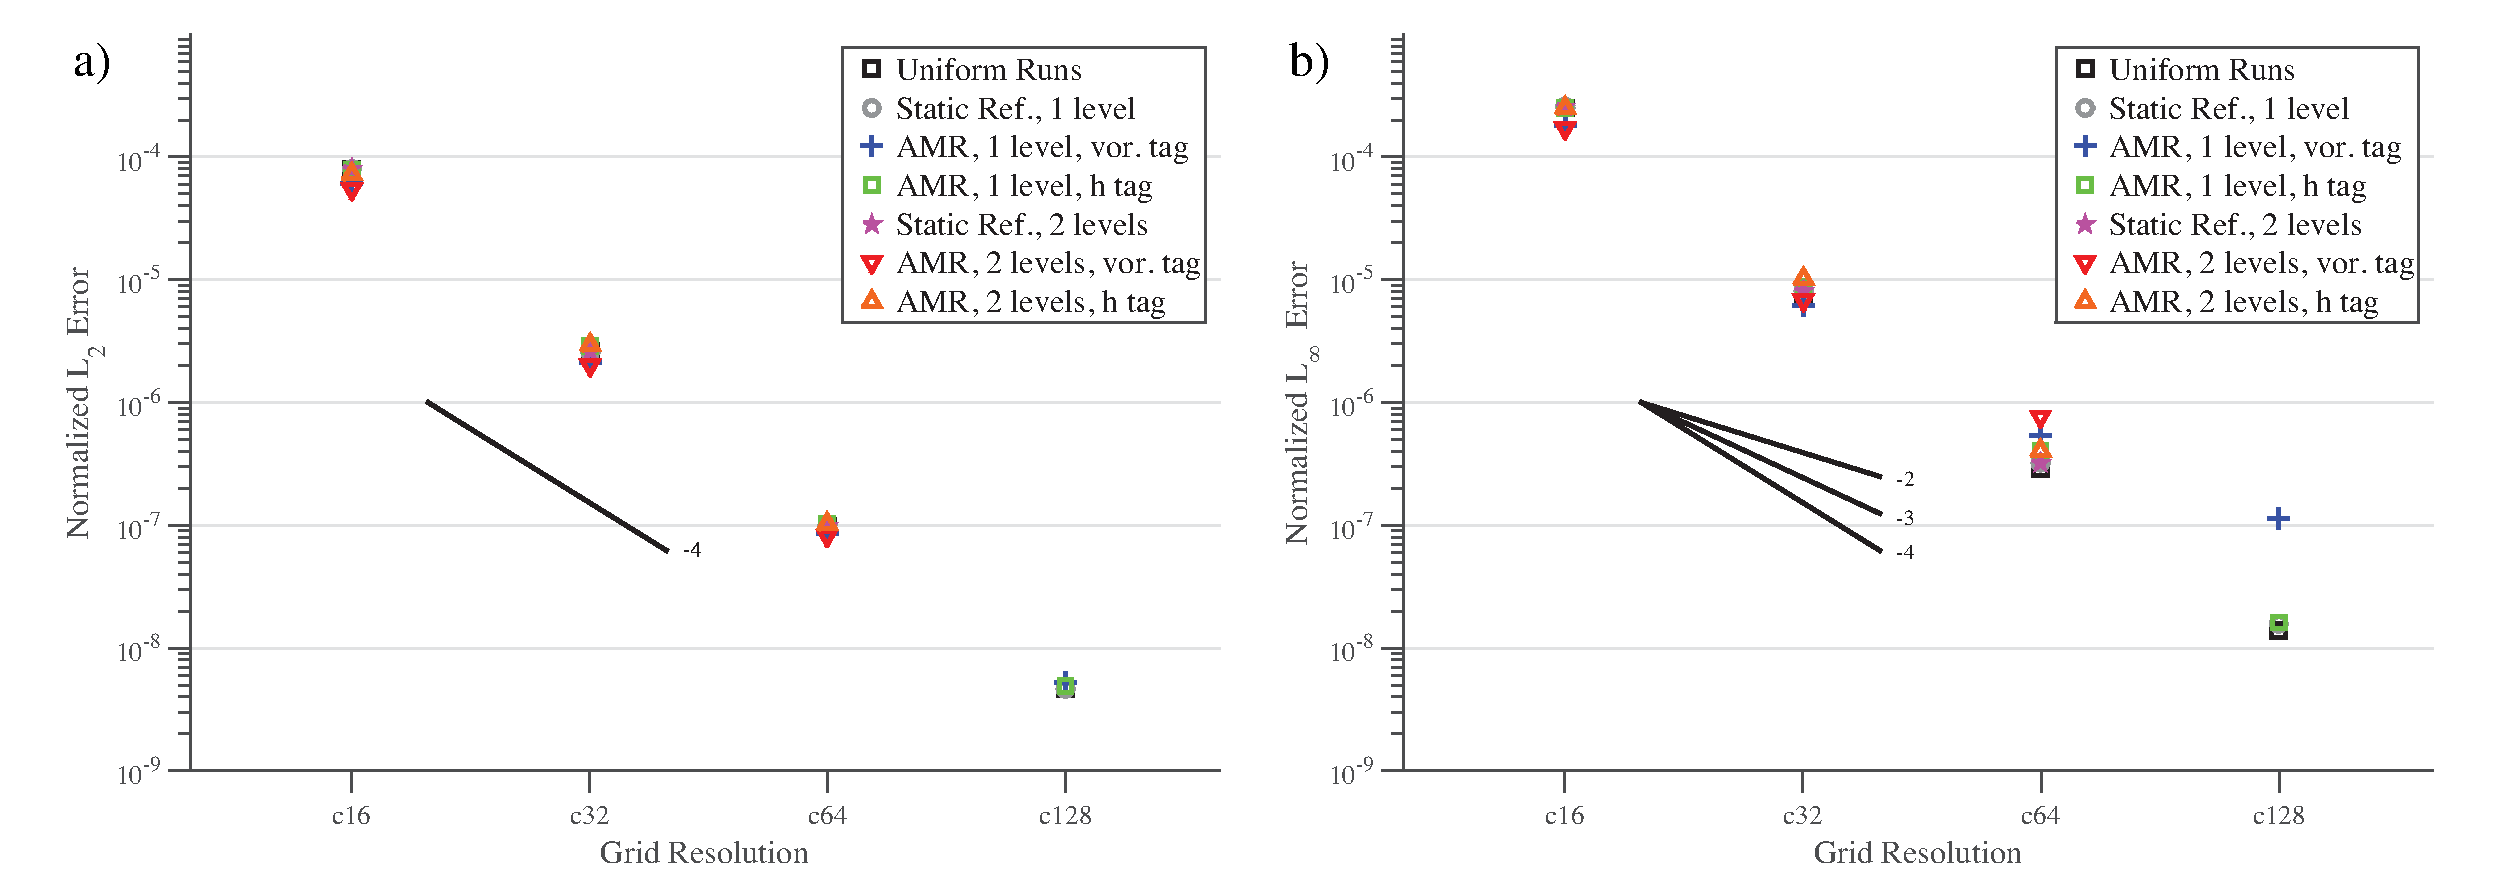
\includegraphics[width=\textwidth]{Chap1/final_USBR_errvgrids_combo}}
    \caption{(a) Normalized $l_2$ and (b) $l_\infty$ height errors
    at day 5 as a function of base grid resolution for the USBR test
    case of
Section~\ref{subsec:usbr}.
    Uniform runs and AMR runs with one and two refinement levels
    using the height-tag or vorticity-tag criteria.  All AMR runs use x4
    refinement ratio between levels.  Solid black lines depict
    convergence rates.  Errors are determined with respect to the
    analytic solution.}%
    \label{fig:usbrconvergeplots}
\end{figure}
%
We performed the USBR test in simulations with increasing base
resolutions of up to c128 ($\sim 78$ km spacing) with the two dynamic grid configurations.  The
normalized $l_2$ and $l_\infty$ height errors after five days are
plotted in 
Figs.~\ref{fig:usbrconvergeplots}a and
\ref{fig:usbrconvergeplots}b, respectively.  At higher base resolutions the slight
improvements in the $l_2$ height error no longer occur for the vorticity-tag AMR as the
large-scale flow features are well resolved (Fig.~\ref{fig:usbrconvergeplots}a).  The fourth-order
convergence is maintained for all grid configurations.  In the $l_\infty$
height error plot
(Fig.~\ref{fig:usbrconvergeplots}b), we observe the same slight decrease in
error for the coarse c16 and c32 base resolutions for the vorticity-tag
AMR and the slight increase in the height-tag AMR errors as observed earlier in
Figs.~\ref{fig:usbrherrplots}c-d.
However, at higher base resolutions we find a
large increase in the $l_\infty$ error for the vorticity-tag AMR runs.  While
fourth-order convergence is maintained at all resolutions for the uniform, static
refinement, and height-tag AMR configurations across all resolutions,
the $l_\infty$ convergence rate drops to between 3 and 2.5 for the vorticity-tag
AMR runs at higher base resolutions.  The increased error is due to the
regridding of the AMR patches.  The maximum errors occur in cells bordering
the coarse-fine boundary of the AMR patch and the base grid when that
boundary intersects an edge of the cubed-sphere.  This point-source-like
artifact of the AMR grid occurs in both the height-tag and vorticity-tag
AMR simulations.  In the height-tag runs, the artifact is triggered only
when the AMR grid passes over the corners of the cubed-sphere,
resulting in the slight $l_\infty$ error increase observed in 
Fig.~\ref{fig:usbrherrplots}c.  In the vorticity-tag AMR runs, the refined
grid bisects the polar-equatorial panel edge during the entire run, thus
this small error is compounded at each regridding step.  This results in
the sharp increase in the $l_\infty$ error seen in 
Fig.~\ref{fig:usbrconvergeplots}b for the vorticity-tag runs with c64 and
c128 base resolutions.  Overall, though, the error is small and very
localized at the cells where the AMR patches intersect the cubed-sphere
edge. It is therefore only obvious in the strict $l_\infty$ error measure and only at 
high horizontal base resolutions. At lower base resolutions the magnitudes of other errors are
bigger which then dominate the global $l_\infty$ error measure.


\subsection{Isolated Mountain Gravity Wave}
\label{subsec:gravity-wave}

This shallow-water test was
developed to assess AMR when topography is present.  In the test a
gravity wave, that is triggered by an unbalanced initial height perturbation in a quiescent background environment, passes over an
idealized mountain.  The change in topography deforms the structure of
the gravity wave.  The bottom topography $z_s$ consists of a cosine mountain
and is defined by
\begin{equation}
    \label{eq:topomount} z_s = \frac{z_0}{4}\left(1+\cos\left(\frac{\pi
    r}{R}\right)\right)^2
\end{equation}
where $R=\pi/9$ and 
$r^2 = \min[R^2, (\lambda-\lambda_c)^2+(\theta - \theta_c)^2]$. Outside the radius $R$ 
the topography is set to zero.  
The peak height of the mountain is $z_0=2000\text{ m}$, and it is
centered at $(\lambda_c,\theta_c)=(3\pi/2,\pi/6)$ in the longitudinal and latitudinal direction, respectively. %
The initial velocity field is set to zero and the initial free surface
height has a constant background value of $h_0=5960 \text{ m}$ with a
local Gaussian dip perturbation.  Thus the initial free surface height field (above the reference sphere at sea level) is given
as
\begin{equation}
    \label{eq:gwmountgauss} h = h_0 - h_{max} \exp{\left(-\left(\frac{\tau}
    {\beta}\right)^2\right)}.
\end{equation}
The maximum depth of the perturbation is set to $h_{max}=100\text{ m}$,
$\beta=\pi/36$ is a width parameter, and $\tau$ is the great-circle distance
from point $(\lambda,\theta)$ to the dip's center $(\lambda_d,\theta_d)$
such that
\begin{equation}
    \label{eq:gc} \tau = a \arccos \left(\sin\theta_d \sin\theta + \cos\theta_d
    \cos\theta \cos\left(\lambda - \lambda_d\right)\right)
\end{equation}
where $a = 6.37122 \times 10^{6}\text{ m}$ is the average radius of
the Earth.  The Gaussian dip is centered at 
$(\lambda_d,\theta_d)=(3\pi/2 - \pi/5, \pi/6)$ in the longitudinal and latitudinal direction, respectively.
Figure~\ref{fig:gw_setup} depicts the initial height field and its distance
from the mountain.
%
\begin{figure}
    \centerline{%
    \noindent
    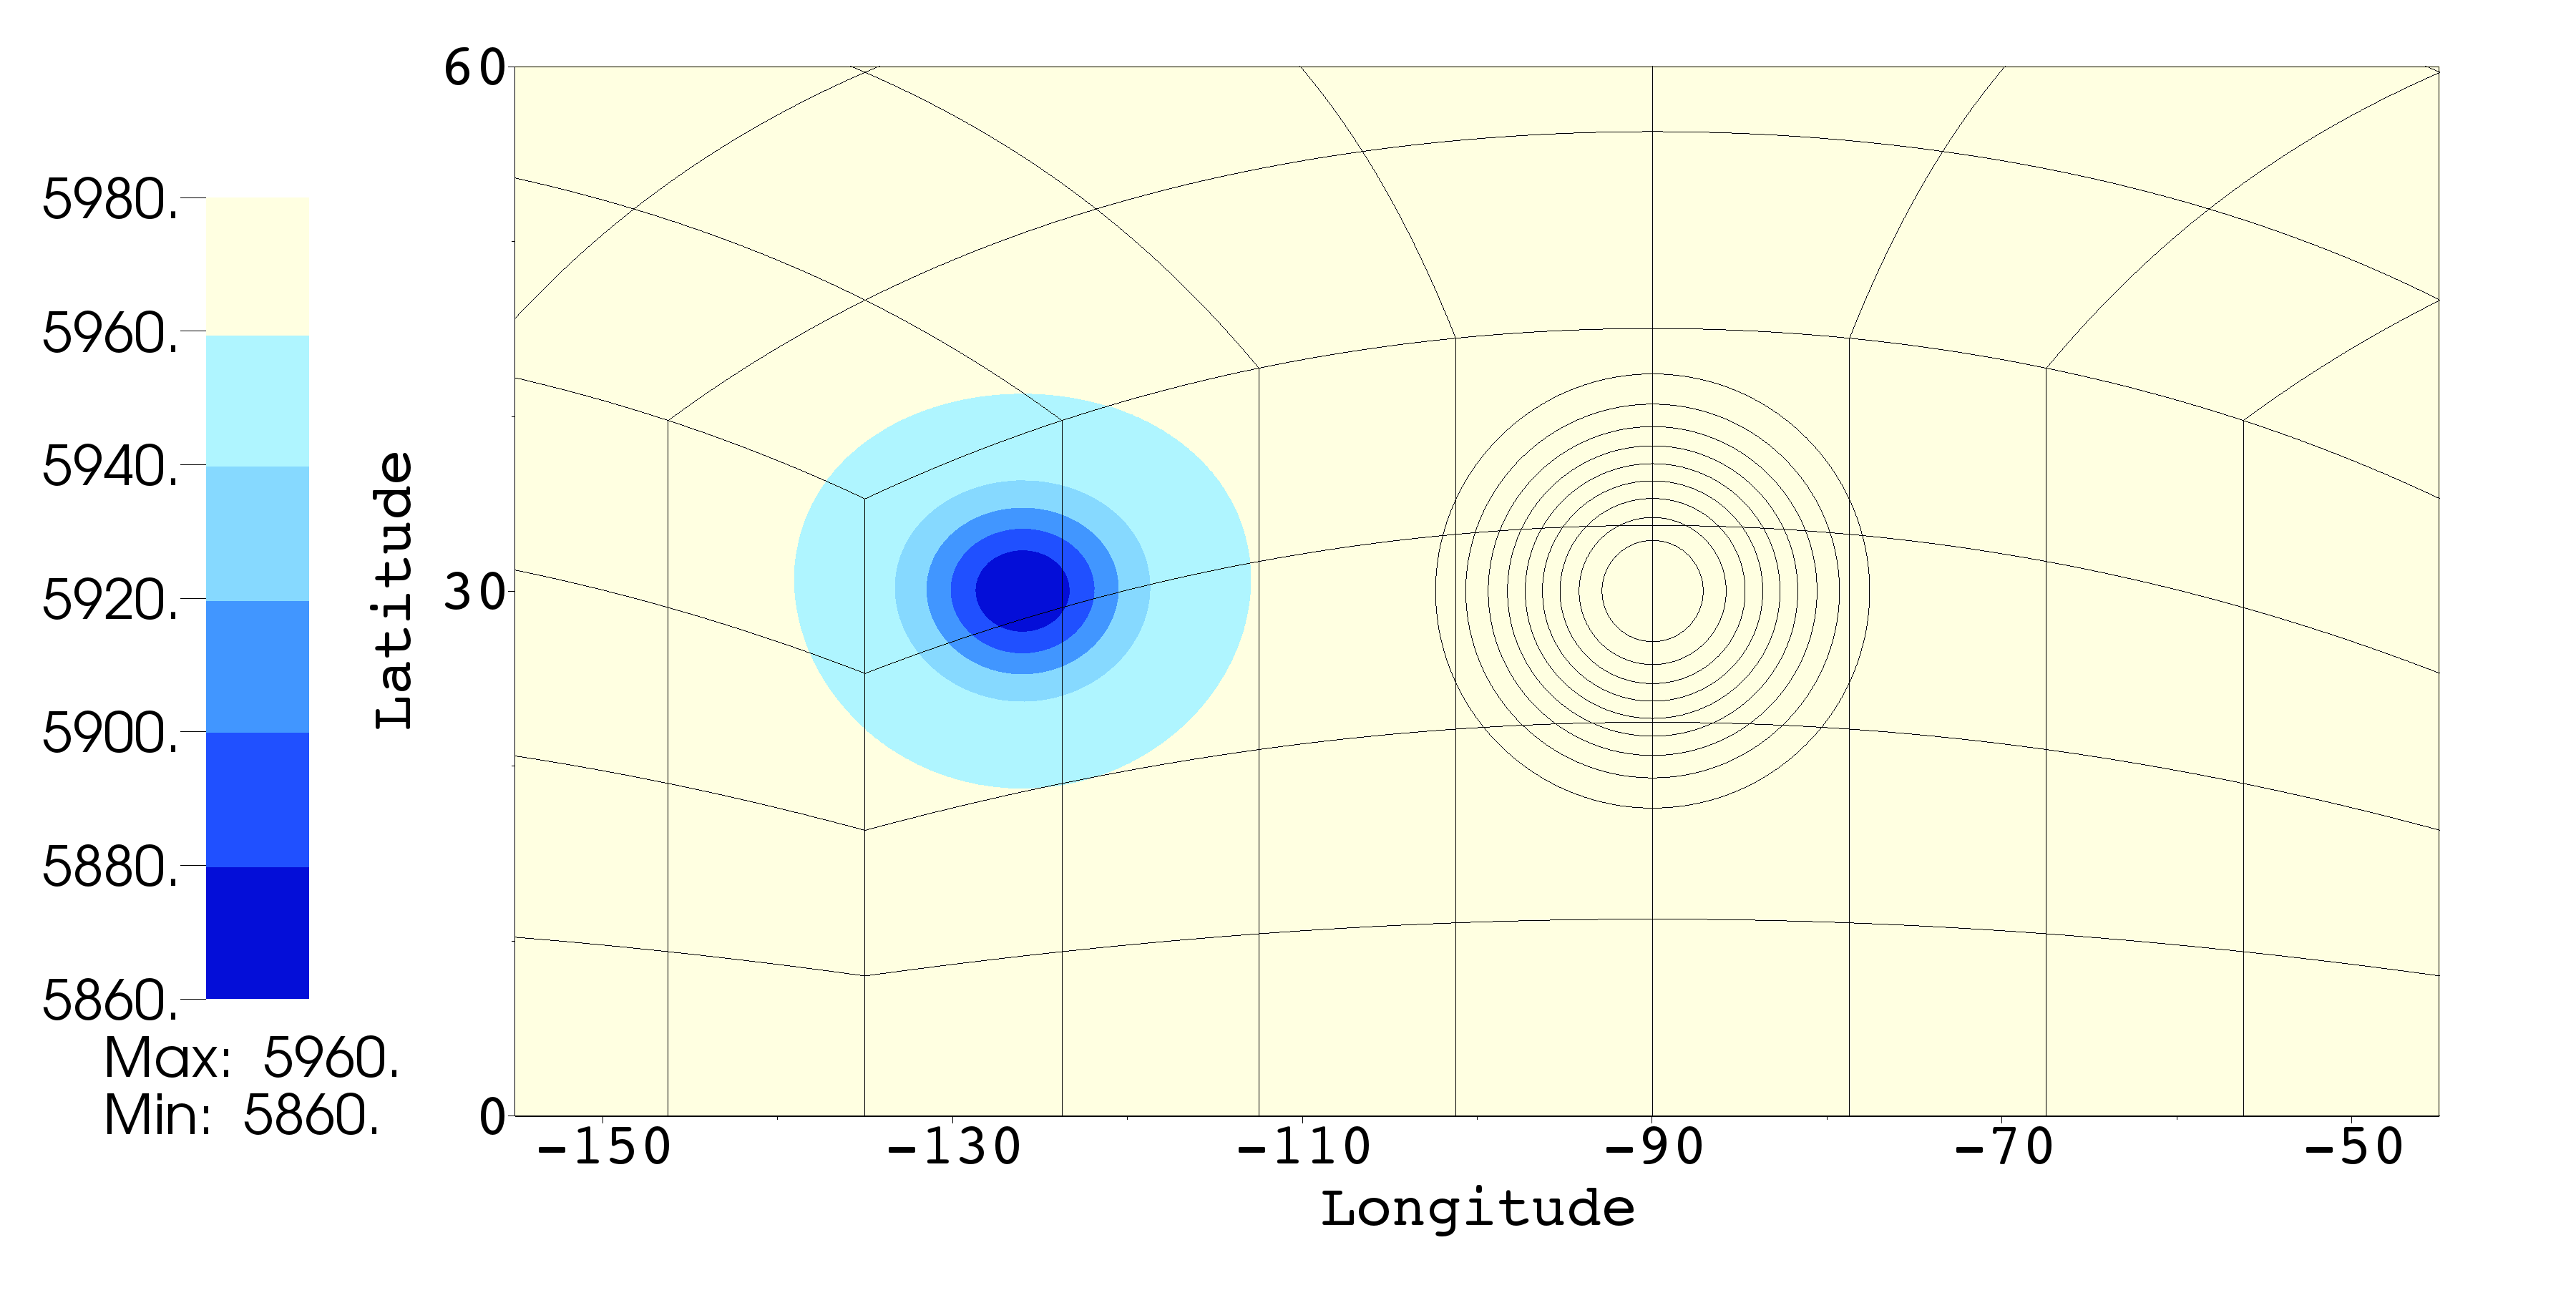
\includegraphics[width=19pc]{Chap1/GW_c256_hpert_flat_hr_00}}
    \caption{Initial free surface height field (colored, in m) for the gravity wave over an idealized
    mountain test of
Section~\ref{subsec:gravity-wave}.
  The free surface height field (above the reference sphere at sea level) is uniform everywhere except for
    the 100 m deep Gaussian depression.  The black contour lines
    represent the location of the mountain with 200 m contour spacing
    and a peak mountain height of 2000 m.}%
    \label{fig:gw_setup}
\end{figure}
%
\begin{figure}
    \centerline{%
    \noindent
    \includegraphics[width=\textwidth]{Chap1/gw_hr_06.eps}}
    \caption{Mountain gravity-wave test of
Section~\ref{subsec:gravity-wave},
 at hour 6.  (a) and (b) depict the
    perturbation height of the gravity wave as it passes over the
    mountain for a uniform c128 run and a c32/c128 AMR run with the height gradient tag 
    $|\nabla h| > 7.5 \times 10^{-6}$,  (c) and (d)
    depict the height error of each run after six hours compared to a
    reference uniform c1024 run.  The block structure of the grid and
    the mountain contours are overlaid with thin black lines.}%
    \label{fig:GW_hr6}
\end{figure}
%
\begin{figure}
    \centerline{%
    \noindent
    \includegraphics[width=\textwidth]{Chap1/gw_hr_12.eps}}
    \caption{Same runs and plots as in 
Fig.~\ref{fig:GW_hr6} except for hour 12 as the gravity wave has moved
    halfway around the sphere.}%
    \label{fig:GW_hr12}
\end{figure}
%
The simulation is run for a period of twelve hours so that the gravity
wave has moved halfway around the sphere.
Figures~\ref{fig:GW_hr6} and
\ref{fig:GW_hr12} show the perturbation height (defined as deviations from $h_0$,
top panels) and the height difference from a uniform c1024 ($\sim 10$ km) reference
solution (bottom panels) at hour 6 and hour 12, respectively, for a
uniform c128 run and a c32 base 1-level AMR run (c32/c128) tagged on a
height-gradient threshold of $|\nabla h| > 7.5 \times 10^{-6}$.  After
six hours (Fig.~\ref{fig:GW_hr6}), the gravity wave has just passed over the mountain
and the distortion to the wave from the mountain is clearly visible.
The presence of the mountain breaks the symmetry of the circular,
outward-propagating gravity wave.  This propagation is captured by the
AMR refinement criterion as indicated by the overlaid block structure in
Figs.~\ref{fig:GW_hr6}b, d.  The height differences for the c32/c128 AMR run (plot
(d) in 
Figs.~\ref{fig:GW_hr6} and
\ref{fig:GW_hr12}) are similar in position and magnitude to the uniform
c128 run errors (plot (c)) within the refined AMR domain.  The areas of
larger error at the borders of the AMR region seen in 
Figs.~\ref{fig:GW_hr6}d and
\ref{fig:GW_hr12}d are located over the leading and trailing edges of
the gravity wave, which are not fully covered by the AMR refinement criterion.  The
location and magnitude of these larger errors correlate with the error
at the leading edge of the gravity wave observed in the uniform c32
run.  At hour 6, the AMR refined grids are over the mountain and by hour
12, the mountain is once again covered by only the coarse grid.  The AMR
reinitializes the topography (using Eq.~(\ref{eq:topomount})) whenever adaptations are triggered.  No spurious
errors appear as the AMR refines and coarsens over the topography region
(Figs.~\ref{fig:GW_hr6}d and \ref{fig:GW_hr12}d).
%
\begin{figure}
    \centerline{%
    \noindent
    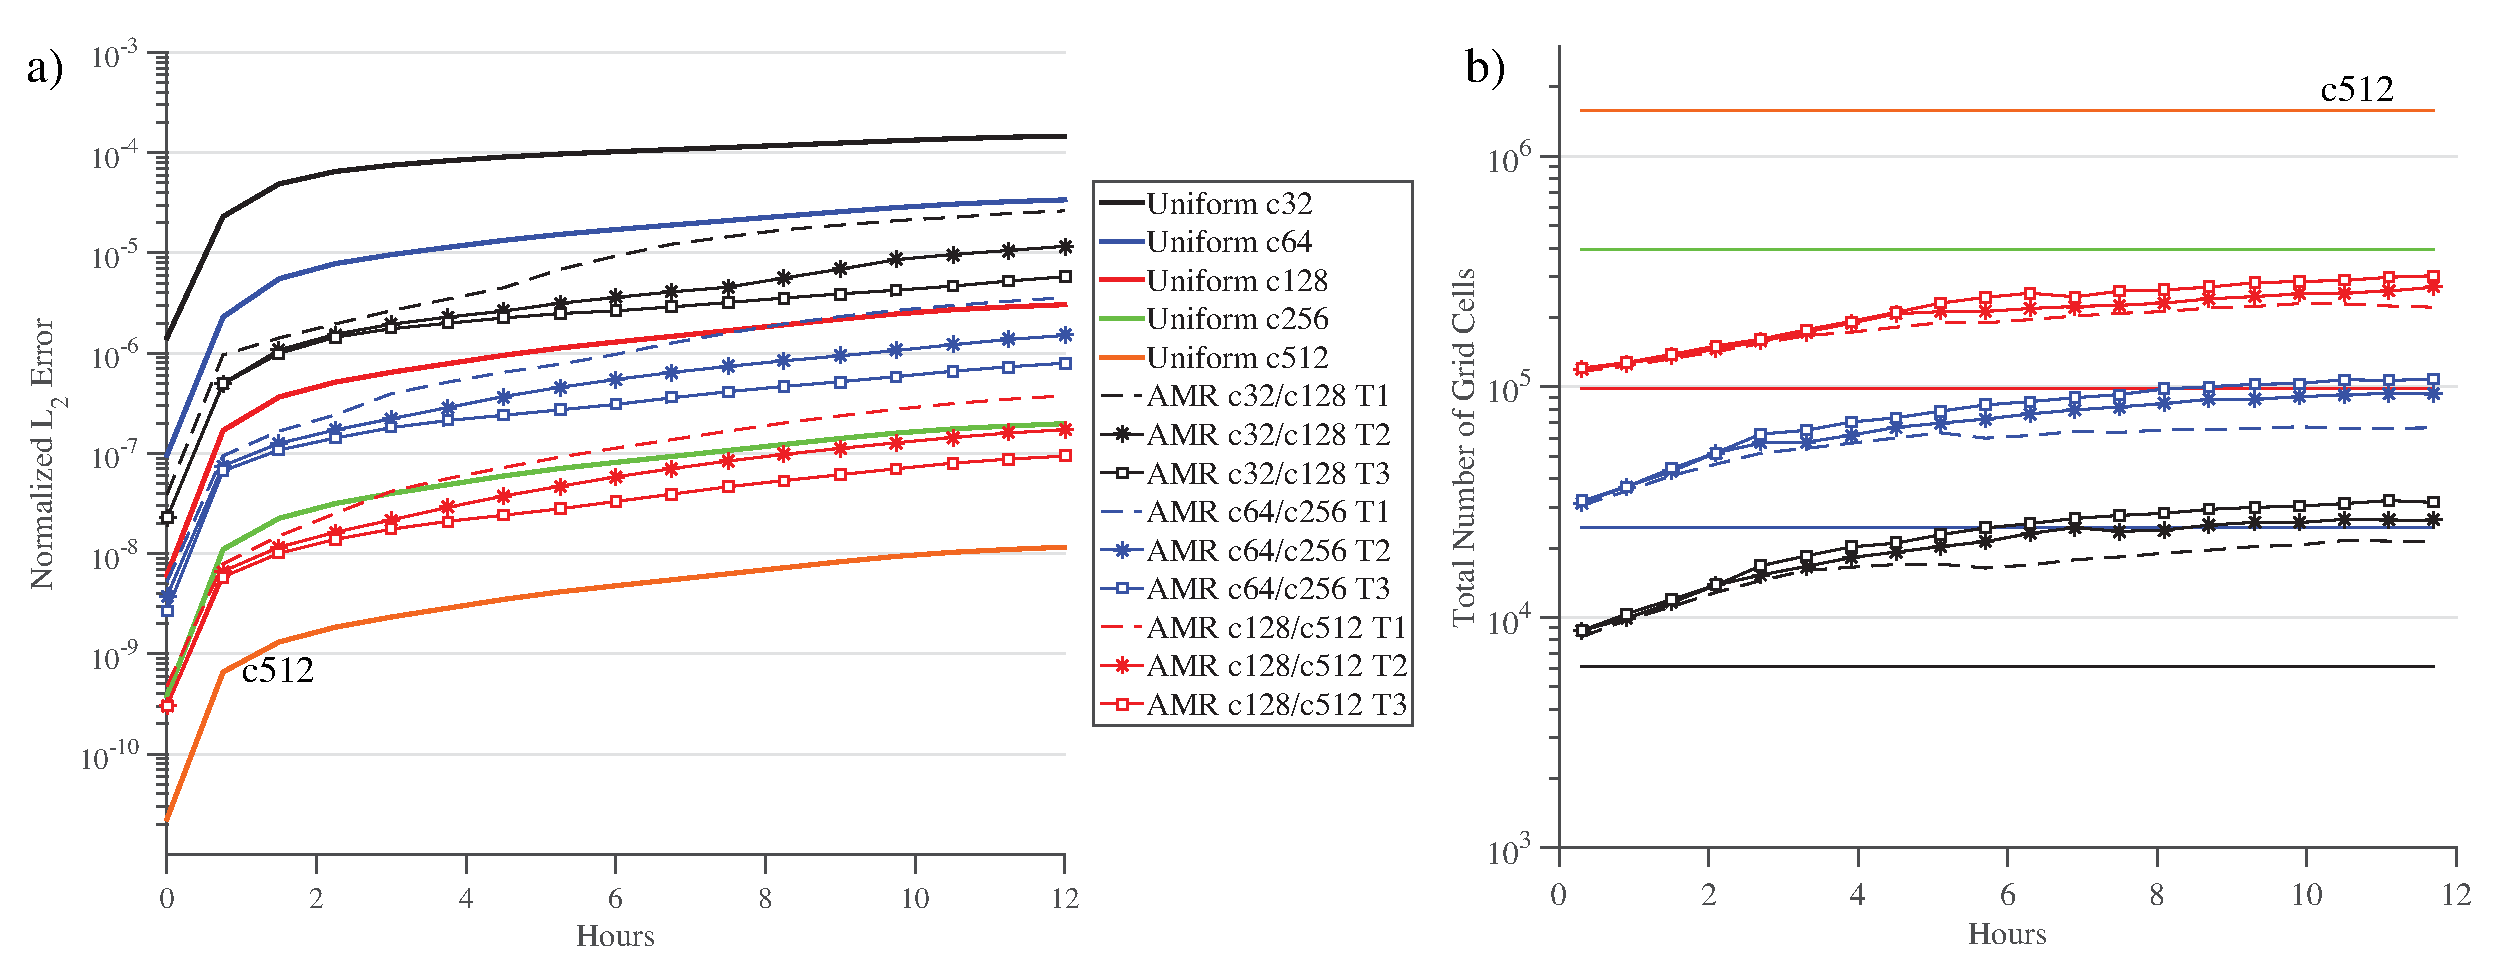
\includegraphics[width=\textwidth]{Chap1/final_gw_l2andgrid_plots.eps}}
    \caption{
For the mountain gravity-wave test of
Section~\ref{subsec:gravity-wave},
growth over the twelve-hour period of:
(a) normalized $l_2$ height error with
    respect to the uniform c1024 run, and (b) total number of grid cells.
    Error and number of grid cells for uniform-resolution runs and 1- and 2- level
    AMR runs with height-gradient tagging. The thresholds are
    $|\nabla h| =1.5\times 10^{-5}$ (T1), $1.0\times 10^{-5}$ (T2), 
    and $7.5 \times 10^{-6}$ (T3).}%
    \label{fig:GW_l2err}
\end{figure}
%
Results in 
Fig.~\ref{fig:GW_l2err} show the normalized $l_2$ height error
(Fig.~\ref{fig:GW_l2err}a) and the total number of grid cells
(Fig.~\ref{fig:GW_l2err}b) as a function of forecast hour for uniform runs from c32 to
c512 and 1-level AMR runs using height-gradient tagging with thresholds
of $|\nabla h| > 1.5\times 10^{-5}$, $1.0\times 10^{-5}$, and 
$7.5 \times 10^{-6}$, labeled T1, T2, and T3, respectively. The normalized error metrics
are determined with respect to the uniform c1024 simulation which serves as the reference solution.  For
uniform runs, the solution error converges to fourth order in both the
normalized $l_2$ and $l_\infty$ height error norms.  The AMR runs
have improved error but do not reach the error of the uniform
run with the same resolution as the highest refinement level.  The c32
base 1-level AMR T3 run (c32/c128) has a maximum number of grid cells
roughly equivalent to the uniform c64 run, but its error is nearly an
order of magnitude smaller than the uniform c64 run.  Reducing the
gradient threshold in AMR runs so that more area around the gravity wave
is covered by the AMR patches improves the solution and reduces error.
A c32/c128 AMR run with a refinement threshold of 
$|\nabla h| > 4.5 \times 10^{-6}$, lower than the T3 criterion, 
results in the AMR grid
covering $31\%$ of the globe by hour 12 and a normalized $l_2$
height error of $3.957\times10^{-6}$.  In comparison, the uniform c128
run has an error of $3.051\times 10^{-6}$ and the T3 run has an error
of $5.806\times 10^{-6}$ with AMR blocks covering only $25.8\%$ of
the area.  As more of the leading edge of the gravity wave is refined
with lower tagging thresholds, the error is decreased further,
though at a diminishing rate.

\subsection{Binary-Vortices Interaction} 
\label{subsec:binary-vortices}

The binary-vortices interaction
test demonstrates the AMR benefits and its
effectiveness in studying an important and more realistic problem.  The
interaction of two neighboring tropical cyclones (TCs) often alters the
structures of the two, leads to complex tracks for the storms, and in some instances
results in a merger of the two cyclones.  These
interactions were first studied by Fujiwhara \citep{fujiwhara1921natural}
and are commonly called the Fujiwhara effect.  Idealized binary-vortex
interactions have been extensively investigated using 2D idealized
models by
\cite{melander1988symmetric},
\cite{waugh1992efficiency},
\cite{Ritchie:1993eu},
\cite{prieto2003classification} and
\cite{Shin:2006kx}.  A majority of the research has been conducted on
two-dimensional Cartesian systems using a constant Coriolis force.
These studies have used a variety of initial vortex profiles featuring
discrete \citep{Ritchie:1993eu} or continuous \citep{bauer2014simulation}
vortices in both symmetric and asymmetric pairs \citep{dritschel1992quantification}.
They demonstrate that slight changes in initial conditions will cause
widely diverging results.  The vortices will either merge or repel each
other depending on the strength, size, and separation distances of the
vortices, and the post-interaction shapes of the vortices will be vastly
different.
\cite{bauer2014simulation} used an \emph{r}-adaptive shallow-water model to
demonstrate that the vortices' tracks are sensitive to initial
conditions and to initial grid resolution.  Given the sensitivity to
resolution, binary-vortex interactions are a well-suited test of AMR.
The steep gradients, localized areas of high vorticity, and complex flow
fields around the vortices are transient and resolution-dependent,
mimicking the multi-scale nature of tropical cyclones.  With this test, we
can evaluate the AMR's ability to refine and track these features of
interest and measure the AMR's accuracy in resolving the vortex
interaction.  It can assess how well the results and errors in AMR runs
match the results of uniform high-resolution runs and can determine the
sensitivity of the vortex tracks to the changing grid resolutions.

In our binary tropical-cyclone-like vortices test, we use the full
shallow-water equations on a spherical grid with a changing Coriolis
parameter, whereas most other published studies use a nondivergent
barotropic model on an \emph{f}-plane.  We also restrict our study to only the
symmetric case so that the two vortices are identical in size and
strength.  The two vortices are initialized near each other and are
allowed to interact over a simulation period of several days.
Two variations of this setup are presented.  In the separation case, the two
vortices orbit around each other and then slowly drift apart.  In the
merger case, the vortices merge.  Our initializations of the continuous
vortex profiles were inspired by the definition of the initial state in
\cite{Holland:1993ij}.  The initial wind and height profiles are derived
from the shallow-water equations in cylindrical coordinates using an
\emph{f}-plane approximation.  The vortex structure is depicted as a radial
perturbation in the geopotential field and is given by
\begin{eqnarray}
    \label{eq:svgeopot} \phi & = & \bar{\phi} - \phi' \\
    \phi' & = & \phi_c\left(1-\exp\left(-\left(\frac{r_m}{r}\right)^b\right)\right)
    \label{eq:geo_perturb}
\end{eqnarray}
where $\bar{\phi} = g \bar{h}$ is the background geopotential with the 
background height $\bar{h} = 4200$ m and the Earth's gravity $g= 9.80616$ m s$^{-2}$,  $\phi'$ denotes the geopotential perturbation, 
$\phi_c$ symbolizes the maximum geopotential perturbation, $r_m$ is the radius of maximum wind, $b$ stands for a scaling
parameter set to 1.5, and $r$ is the great-circle distance from point 
$(\theta ,\lambda)$ to the vortex center $(\theta_c,\lambda_c)$ (see also Eq.~(\ref{eq:gc})).  The values of 
$\phi_c$, $r_m$, $\theta_c$ and $\lambda_c$ are provided later.

A balanced tangential wind field is then found by using the
steady-state shallow-water momentum equations in cylindrical coordinates.  In particular, 
the tangential wind
\begin{eqnarray}
    v_T = -\frac{r f}{2} \pm \sqrt{\frac{r^2 f^2}{4}+r\frac{\partial
    \phi}{\partial r}}. 
    \label{eq:vt_general}
\end{eqnarray}
represents the initial axisymmetric flow in gradient wind balance.
Using $\partial \phi / \partial r$ derived from Eq.~(\ref{eq:svgeopot}), we get the corresponding tangential velocity for a cyclonic ($+$ sign in Eq.~(\ref{eq:vt_general})) circulation
\begin{eqnarray}
    \label{eq:symvortTv} v_T = \sqrt{\phi_c b \left(\frac{r_m}{r}\right)^b
    \exp\left(-\left(\frac{r_m}{r}\right)^b\right) + \frac{r^2 f^2}{4}}
    - \frac{r f}{2}
\end{eqnarray}
where $f$ is the constant Coriolis parameter for an \emph{f}-plane
approximation at the latitude of the vortex center (specified later).
The last initialization step is to project the tangential velocity onto the sphere with the zonal, $u$,
and meridional, $v$, spherical wind components given by
\begin{eqnarray}
    \label{eq:symvoruv} u = v_T\frac{d_1}{d} \quad\mathrm{and}\quad v =
    v_T\frac{d_2}{d}
\end{eqnarray}
where
\begin{eqnarray}
    d_1 & = & \sin\theta_c \cos\theta - \cos\theta_c \sin\theta\cos\left
    (\lambda - \lambda_c\right) \\
    d_2 & = & \cos\theta_c \sin\left(\lambda - \lambda_c\right) \\
    d & = & \max\left(\epsilon, \sqrt{{d_1}^2+{d_2}^2}\right).
\end{eqnarray}
The threshold value $\epsilon=10^{-25}$ prevents division by zero. The topography is set to zero. 

This initialization technique represents a perfect balance for a single vortex in cylindrical coordinates and leads to a
very good balance in spherical coordinates. Note that the perfect balance is broken on the sphere since
$f$ varies in the spherical domain and is held constant for the purpose of the initialization. In addition,
an analytically derived balance is not fully balanced in a numerical (discrete) sense and
 the overlap region of two vortices is not strictly balanced either. 
 However, the initial imbalances for our separation and 
 merger test cases are very minor and the resulting small gravity waves do not
interfere with our AMR analysis. The same initialization technique was
also used for idealized tropical cyclone simulations in 3D GCMs \citep{reed2011vortex}.
%
\begin{figure}
    \centerline{%
    \noindent
    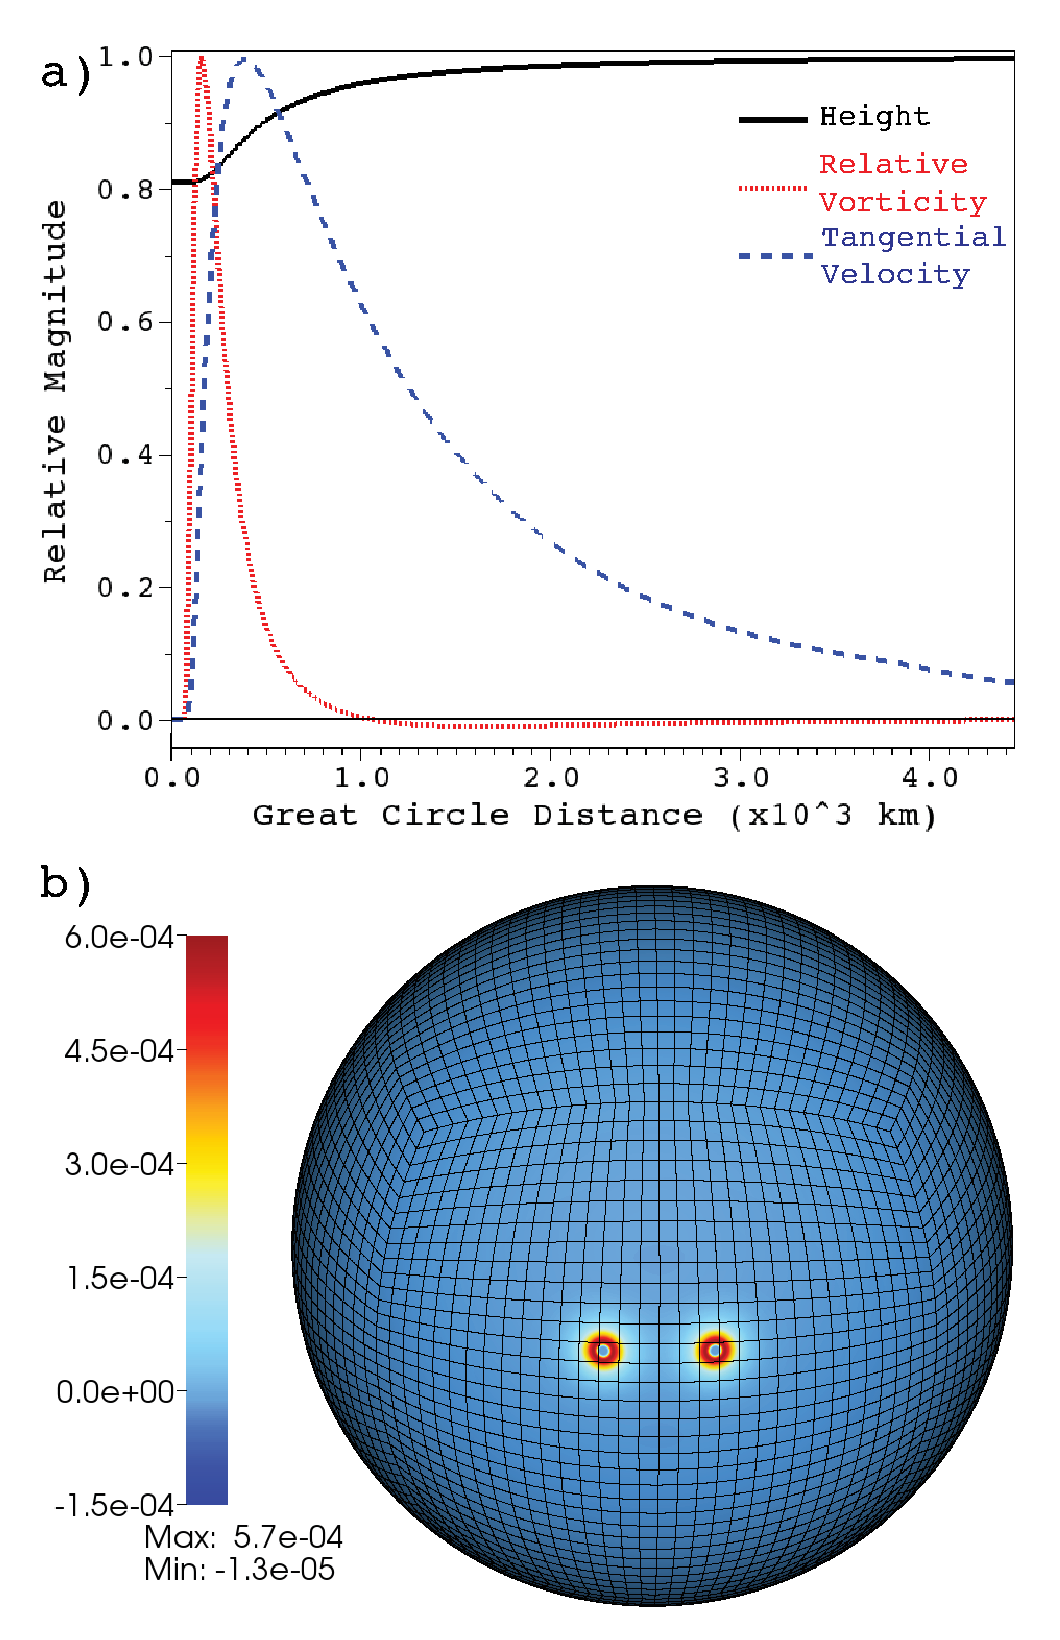
\includegraphics[width=19pc]{Chap1/bvort_setup.eps}}
    \caption{Initial conditions for the binary-vortices test case of
Section~\ref{subsec:binary-vortices}.
    (a) Radial profiles of relative vorticity (red), tangential wind (blue) and
    height field (black) as a function of great-circle distance from the
    center for a single vortex.  Profiles are scaled to the maximum of each
    value (see text).  (b) Initial profile of relative vorticity
    ($\mathrm{s}^{-1}$) of the two vortices on a cubed-sphere grid (merger test case).}%
    \label{fig:bvort_setup}
\end{figure}
%
The radial cross sections of the initial relative vorticity, height field, and tangential wind for a single vortex as a 
function of the great-circle distance from the center are depicted in 
Fig.~\ref{fig:bvort_setup}a.  Here, all magnitudes are
normalized to one and are provided below for each test case.  The initial
relative vorticity for the merger test case with two initial vortices is depicted in 
Fig.~\ref{fig:bvort_setup}b.  It shows that the tangential wind profile from
Eq.~(\ref{eq:symvortTv}) results in a relative vorticity profile with a core of
positive relative vorticity in the center of each storm surrounded 
by a broad ring of negative vorticity with relatively small magnitudes. 
The two vortices slightly overlap with very 
minor magnitudes of u, v and $\phi'$ (Eq.~(\ref{eq:geo_perturb}). 
Here, we use the sum of the $u$, $v$ and $\phi'$ values of both 
vortices to initialize our shallow-water system.


\subsubsection{Separation Case}
\label{subsubsec:separation}

In the separation case, the two vortices
are centered at $\theta_c= \pi/36 = 5^\circ$N which defines the constant Coriolis parameter 
$f = 2 \Omega \sin\theta_c$ with the Earth's angular velocity $\Omega = 7.292 \times 10^{-5}$ s$^{-1}$. The maximum geopotential perturbation is set to
$\phi_c = g h_c$ with the maximum height perturbation $h_c=800$ m.
The radius of maximum wind is set to $r_m=250$ km.  This results
in a maximum tangential wind of $64 \text{ m s}^{-1}$ and a maximum
relative vorticity of $9.4 \times 10^{-4} \text{ s}^{-1}$.  The centers
of the two vortices are $13.5^\circ$ apart ($\sim 1500$ km) in the longitudinal direction, six
times the radius of maximum wind, so that their negative vorticity
regions still overlap.  In particular, the two vortex centers are located at 
$\lambda_{c_1} = (3\pi/2 - 6.75 \pi/180)$ and $\lambda_{c_2} = (3\pi/2 + 6.75\pi/180)$ with 
the midway point between the two cyclones at  $90^\circ$W.

This scenario is sensitive to variations in
initial conditions, making it desirable for testing adaptive grids.
Decreasing the separation distance by 20 km results in the merger of the
two vortices.  During the first three days of the simulation, the two vortices 
make one complete orbit around each other as the beta-drift steers them
towards the northwest, after which the two vortices then drift apart.
In that time, the negative vorticity is stretched as it is advected
around the pair of positive cores before being spun off behind the pair
as an anti-cyclone.  We also observed the growth of a large-scale wave
train that forms in the lee of the orbiting pair.  The time evolution of
the flow can be seen in 
Fig.~\ref{fig:lsplit_uni}, which shows the vorticity field of the cyclone
pair at day 1, 2, 3, 4 and 6 for several uniform-resolution runs.  These serve as
references for the AMR simulations.  We ran uniform runs with
resolutions from c32 through c1024, of which the c128, c256, and c1024
runs are depicted in 
Fig.~\ref{fig:lsplit_uni}.  Results vary significantly with resolution,
though results do converge with increasing resolution.  Runs with
coarser resolution than c128 (not shown) have very weak vortices that
merge instead of drifting apart.  In the c128 run
(Figs.~\ref{fig:lsplit_uni}k--o), the vortices start separating earlier and at
the end of the run are in markedly different positions.  The c256
simulation
(Figs.~\ref{fig:lsplit_uni}f--j) more closely resembles the highest resolution
c1024 run
(Figs.~\ref{fig:lsplit_uni}a--e), but there are still significant differences.
However, the c512 run (not shown as a time series) is nearly indistinguishable from c1024 with only
slight differences in the center of the vortex cores and in the
fine-scale vorticity filaments.  A comparison of the uniform c512 run
and c1024 run at day 6 can be seen in 
Figs.~\ref{fig:lsplit_amr}e and \ref{fig:lsplit_amr}i.
%
\begin{figure}
    \centerline{%
    \noindent
    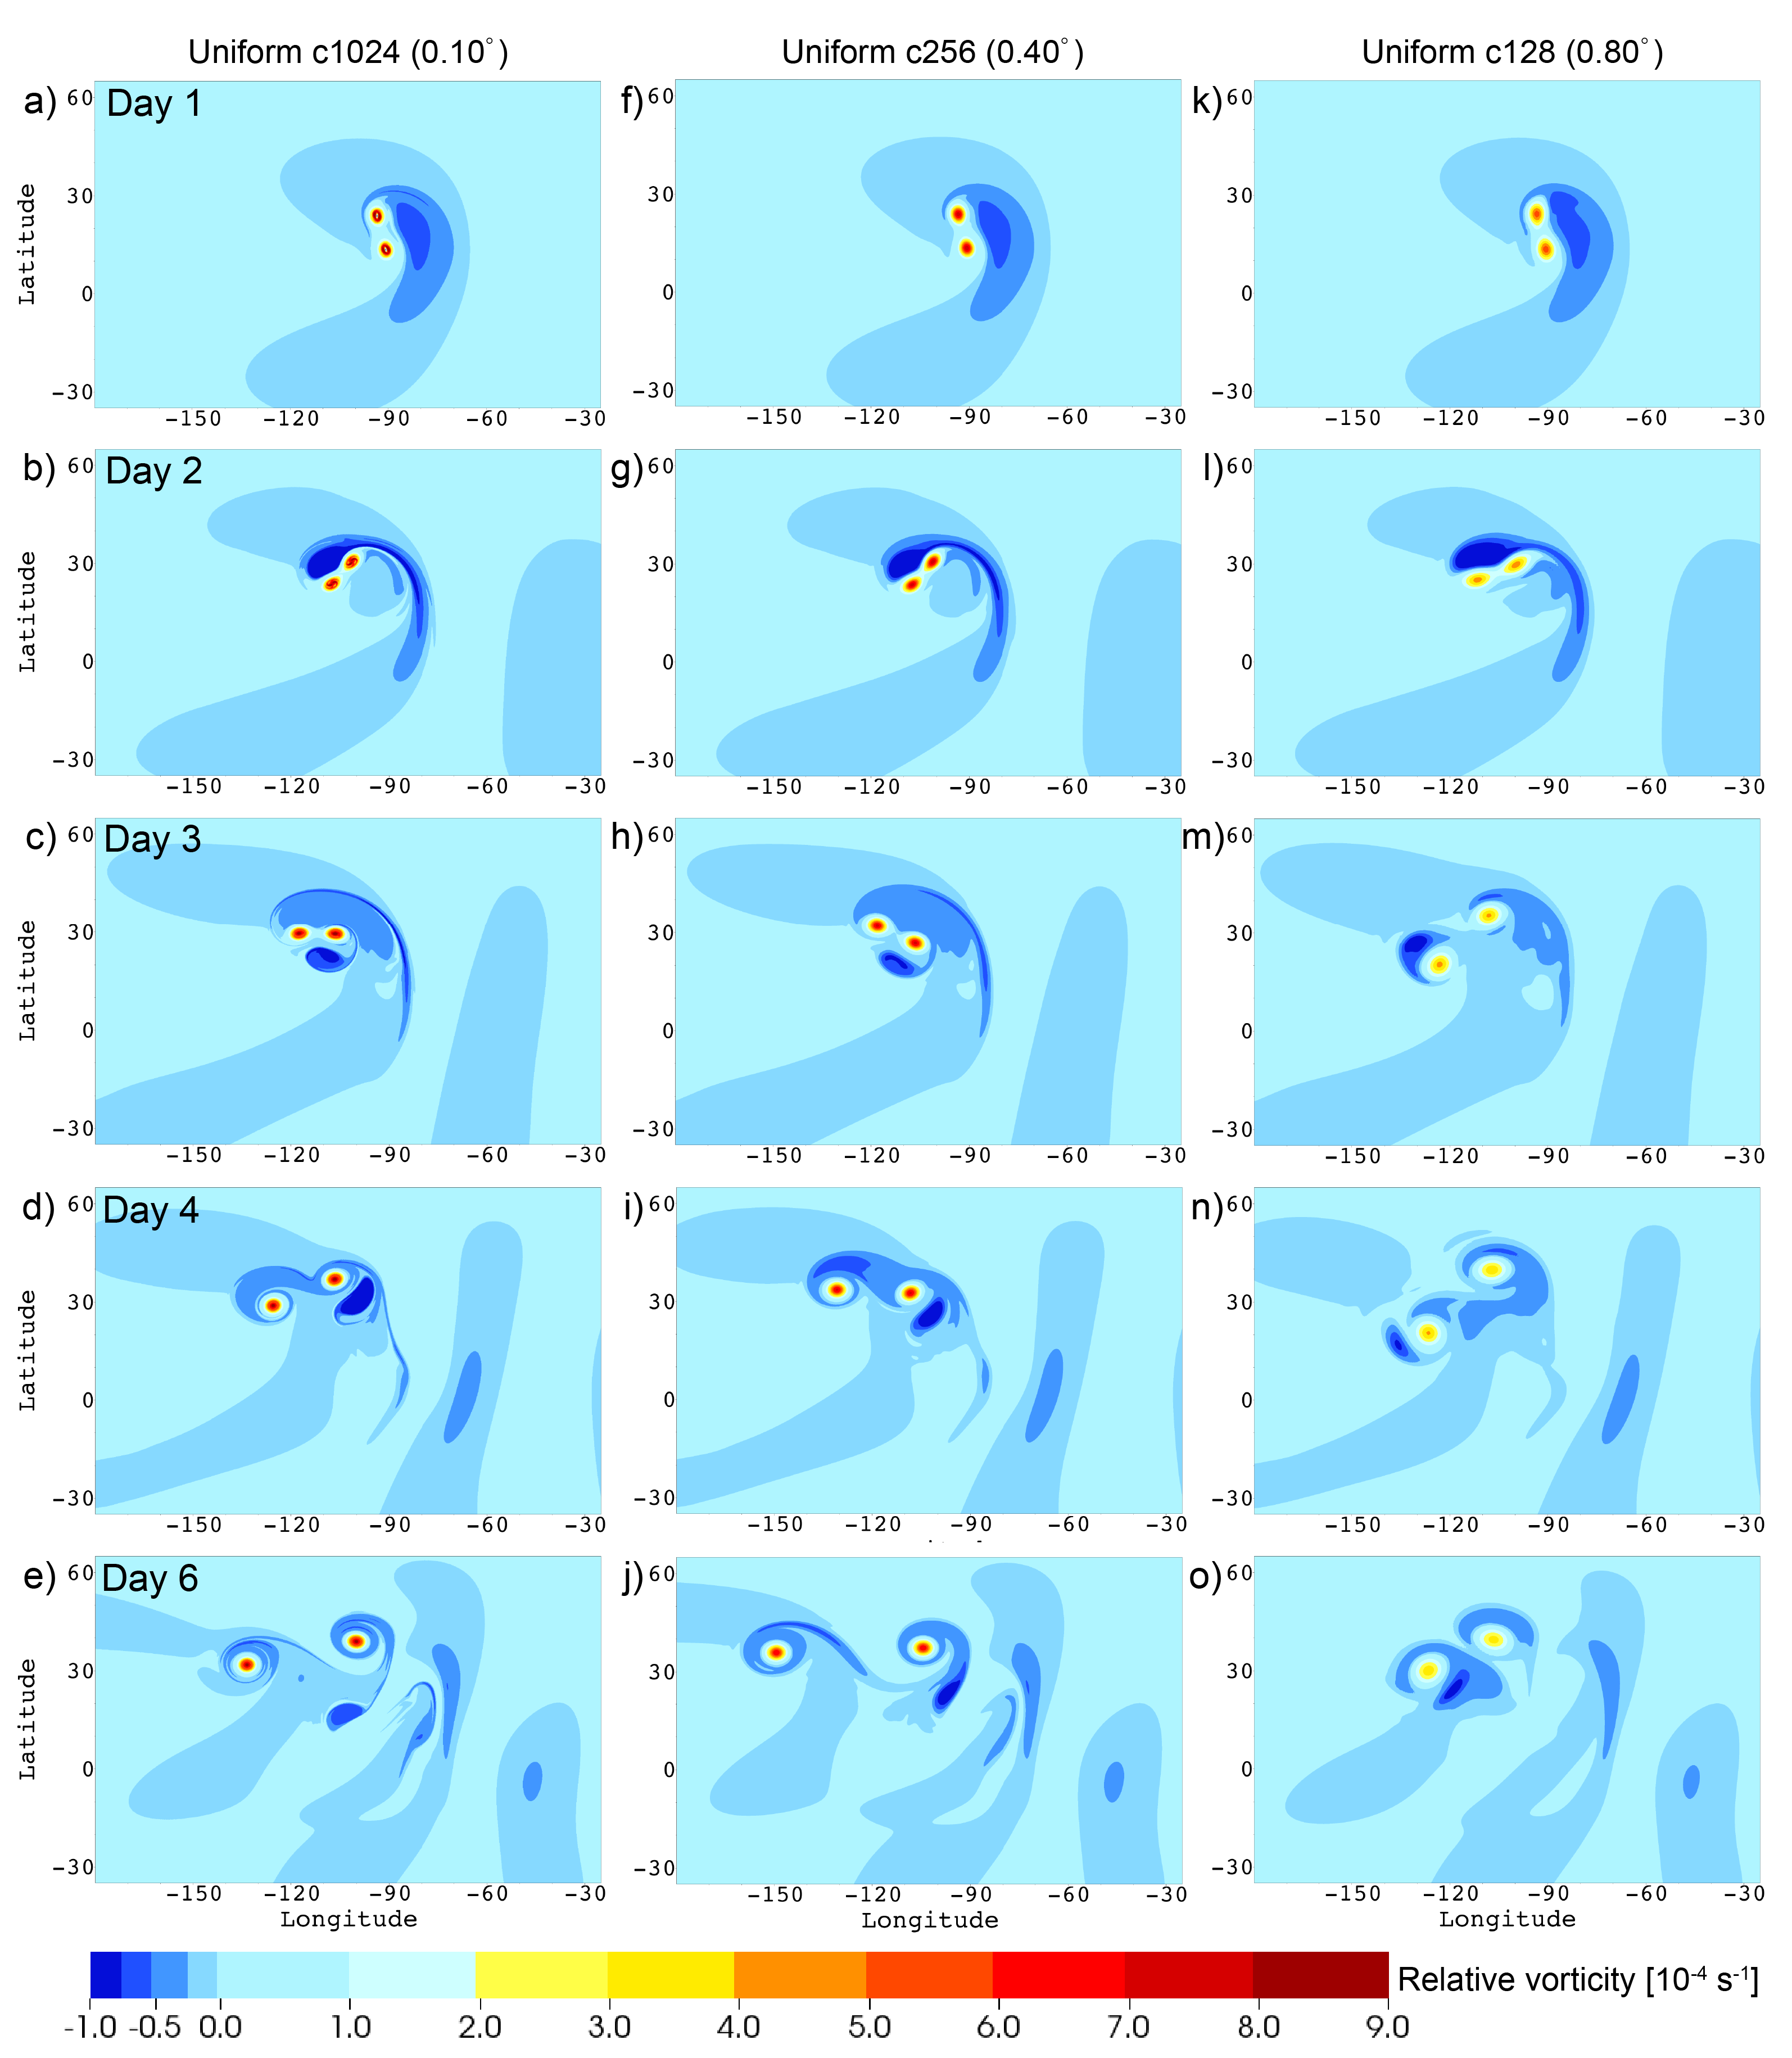
\includegraphics[width=\textwidth]{Chap1/new_uniform_lsplit}}
    \caption{Evolution of the relative vorticity of uniform-resolution runs
    for the binary-vortices test (separation case) of
Section~\ref{subsubsec:separation}.
  (a)--(e) Results for
    the uniform c1024 run for days 1, 2, 3, 4, and 6.  (f)--(j) The
    uniform c256 run and (k)--(o) uniform c128 run.}%
    \label{fig:lsplit_uni}
\end{figure}
%
\begin{figure}
    \centerline{%
    \noindent
    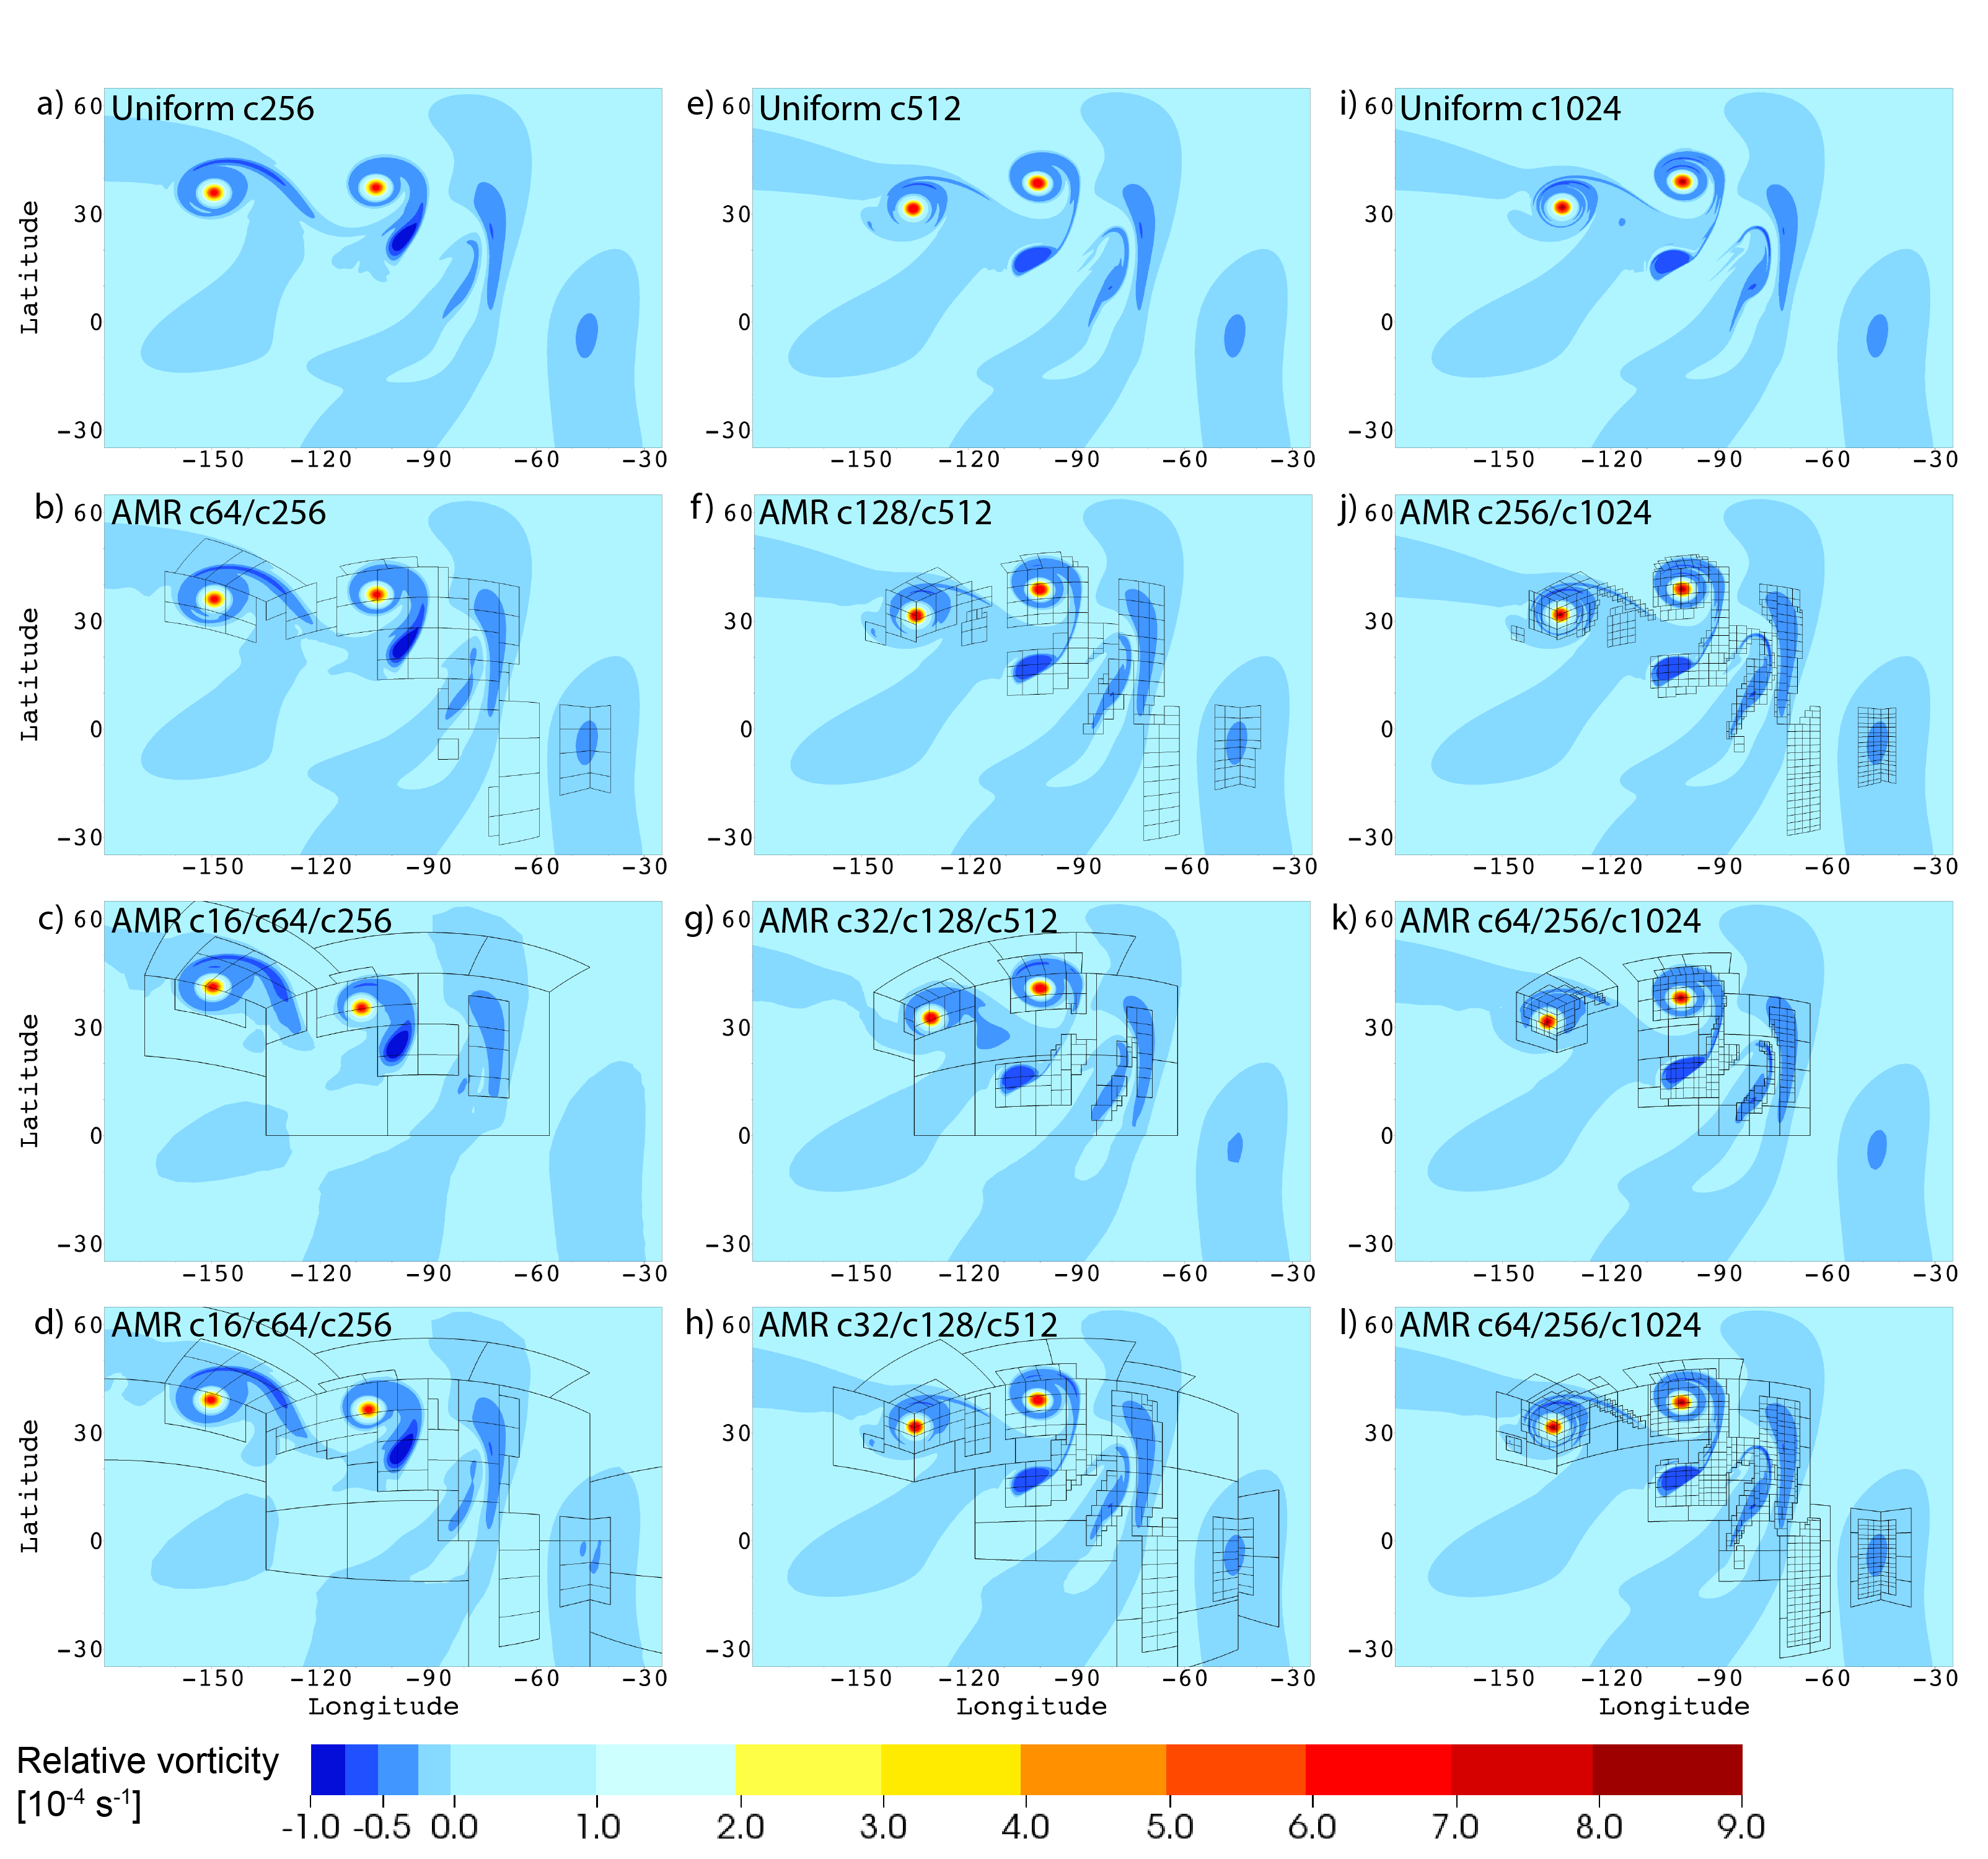
\includegraphics[width=\textwidth]{Chap1/new_lsplit_amr}}
    \caption{Relative vorticity fields at day 6 for several runs of the
    vortex separation case of
Section~\ref{subsubsec:separation}
using AMR.  (a) uniform c256 run, (e) uniform
    c512 run, and (i) uniform c1024 run.  (b), (c), and (d) are AMR runs
    whose highest refinement level is c256.  (f) through (h) and (j)
    through (l) are AMR runs with a highest refinement level of c512 and
    c1024, respectively.  (b), (f), and (j) depict AMR runs with one
    level of refinement using a tagging criterion based on a relative
    vorticity threshold of $|\zeta| > 2.3 \times 10^{-5} \mathrm{ s}^{-1}$.
    (c), (g), and (k) depict AMR runs using two levels of refinement
    using a relative-vorticity threshold of 
    $|\zeta| > 3.5 \times 10^{-5} \mathrm{ s}^{-1}$.  
    The last row, (d), (h), and (l) depict AMR
    runs using the same refinement criteria as the second row but with
    two levels of refinement.  All AMR runs use the x4 refinement
    ratio.  The block structure of refinement levels 1 and 2 are
    outlined in black.}%
    \label{fig:lsplit_amr}
\end{figure}
%
To assess the AMR performance, we ran the model using relative vorticity
refinement criteria with one and two levels of AMR and x4 refinement on
base grid resolutions from c16 to c256.  Samples of the resulting
relative vorticity fields at day 6 using two different
relative vorticity thresholds of $|\zeta| > 3.5 \times 10^{-5} \mathrm{ s}^{-1}$
and $|\zeta| > 2.3 \times 10^{-5} \mathrm{ s}^{-1}$ are displayed in
Fig.~\ref{fig:lsplit_amr}.  They are divided into columns that share the same
highest resolutions, e.g.~in the leftmost column, 
Fig.~\ref{fig:lsplit_amr}a is the uniform c256 run, while 
Figs.~\ref{fig:lsplit_amr}b-d are for 1- or 2-level AMR runs that have a
finest grid resolution of c256.  The AMR runs agree well with the
uniform solutions having the same resolution as the finest AMR level.
The AMR blocks accurately capture the positions of the two vortices and
the shape of their high-vorticity cores.  The AMR runs also effectively
reproduce the overall shapes of the anti-cyclonic filaments and patches
around the cores, and the wave train developing to the lee of the
vortices with only minor differences in the anti-cyclone filament
between the two vortices in a few runs.  Given the nonlinear sensitivity
to initial conditions and grid resolution, unrefined areas and the
coarse-fine boundaries near the vortices in AMR runs may cause divergent
solutions.  In none of our AMR simulations did this occur. The results
of the AMR runs differed only slightly from the uniform-resolution runs.

\subsubsection{Merging Vortices}
\label{subsubsec:merging-vortices}

In the merging-vortices case, the two
vortices have the same maximum height perturbation with $h_c =800$ m, but the radius of maximum
wind is increased to $r_m=400$ km so that the maximum tangential wind
is $61 \text{ m s}^{-1}$ and the maximum relative vorticity is around 
$5.7\times 10^{-4}\text{ s}^{-1}$.  The vortices are centered at $\theta_c= \pi/18 = 10^\circ$N  
where the constant Coriolis parameter $f$ is evaluated for this test case. The vortex centers centers are $15.65^\circ$ 
apart ($\sim 1700$ km) in the longitudinal direction. In particular, they are located at 
$\lambda_{c_1} = (3\pi/2 - 7.825\pi/180)$ and $\lambda_{c_2} = (3\pi/2 + 7.825\pi/180)$ with 
the same midway point as before at $90^\circ$W.
This separation distance is about 4.3
times the radius of maximum wind, so that the edges of the positive
vorticity cores slightly overlap.

%
\begin{figure}
    \centerline{%
    \noindent
    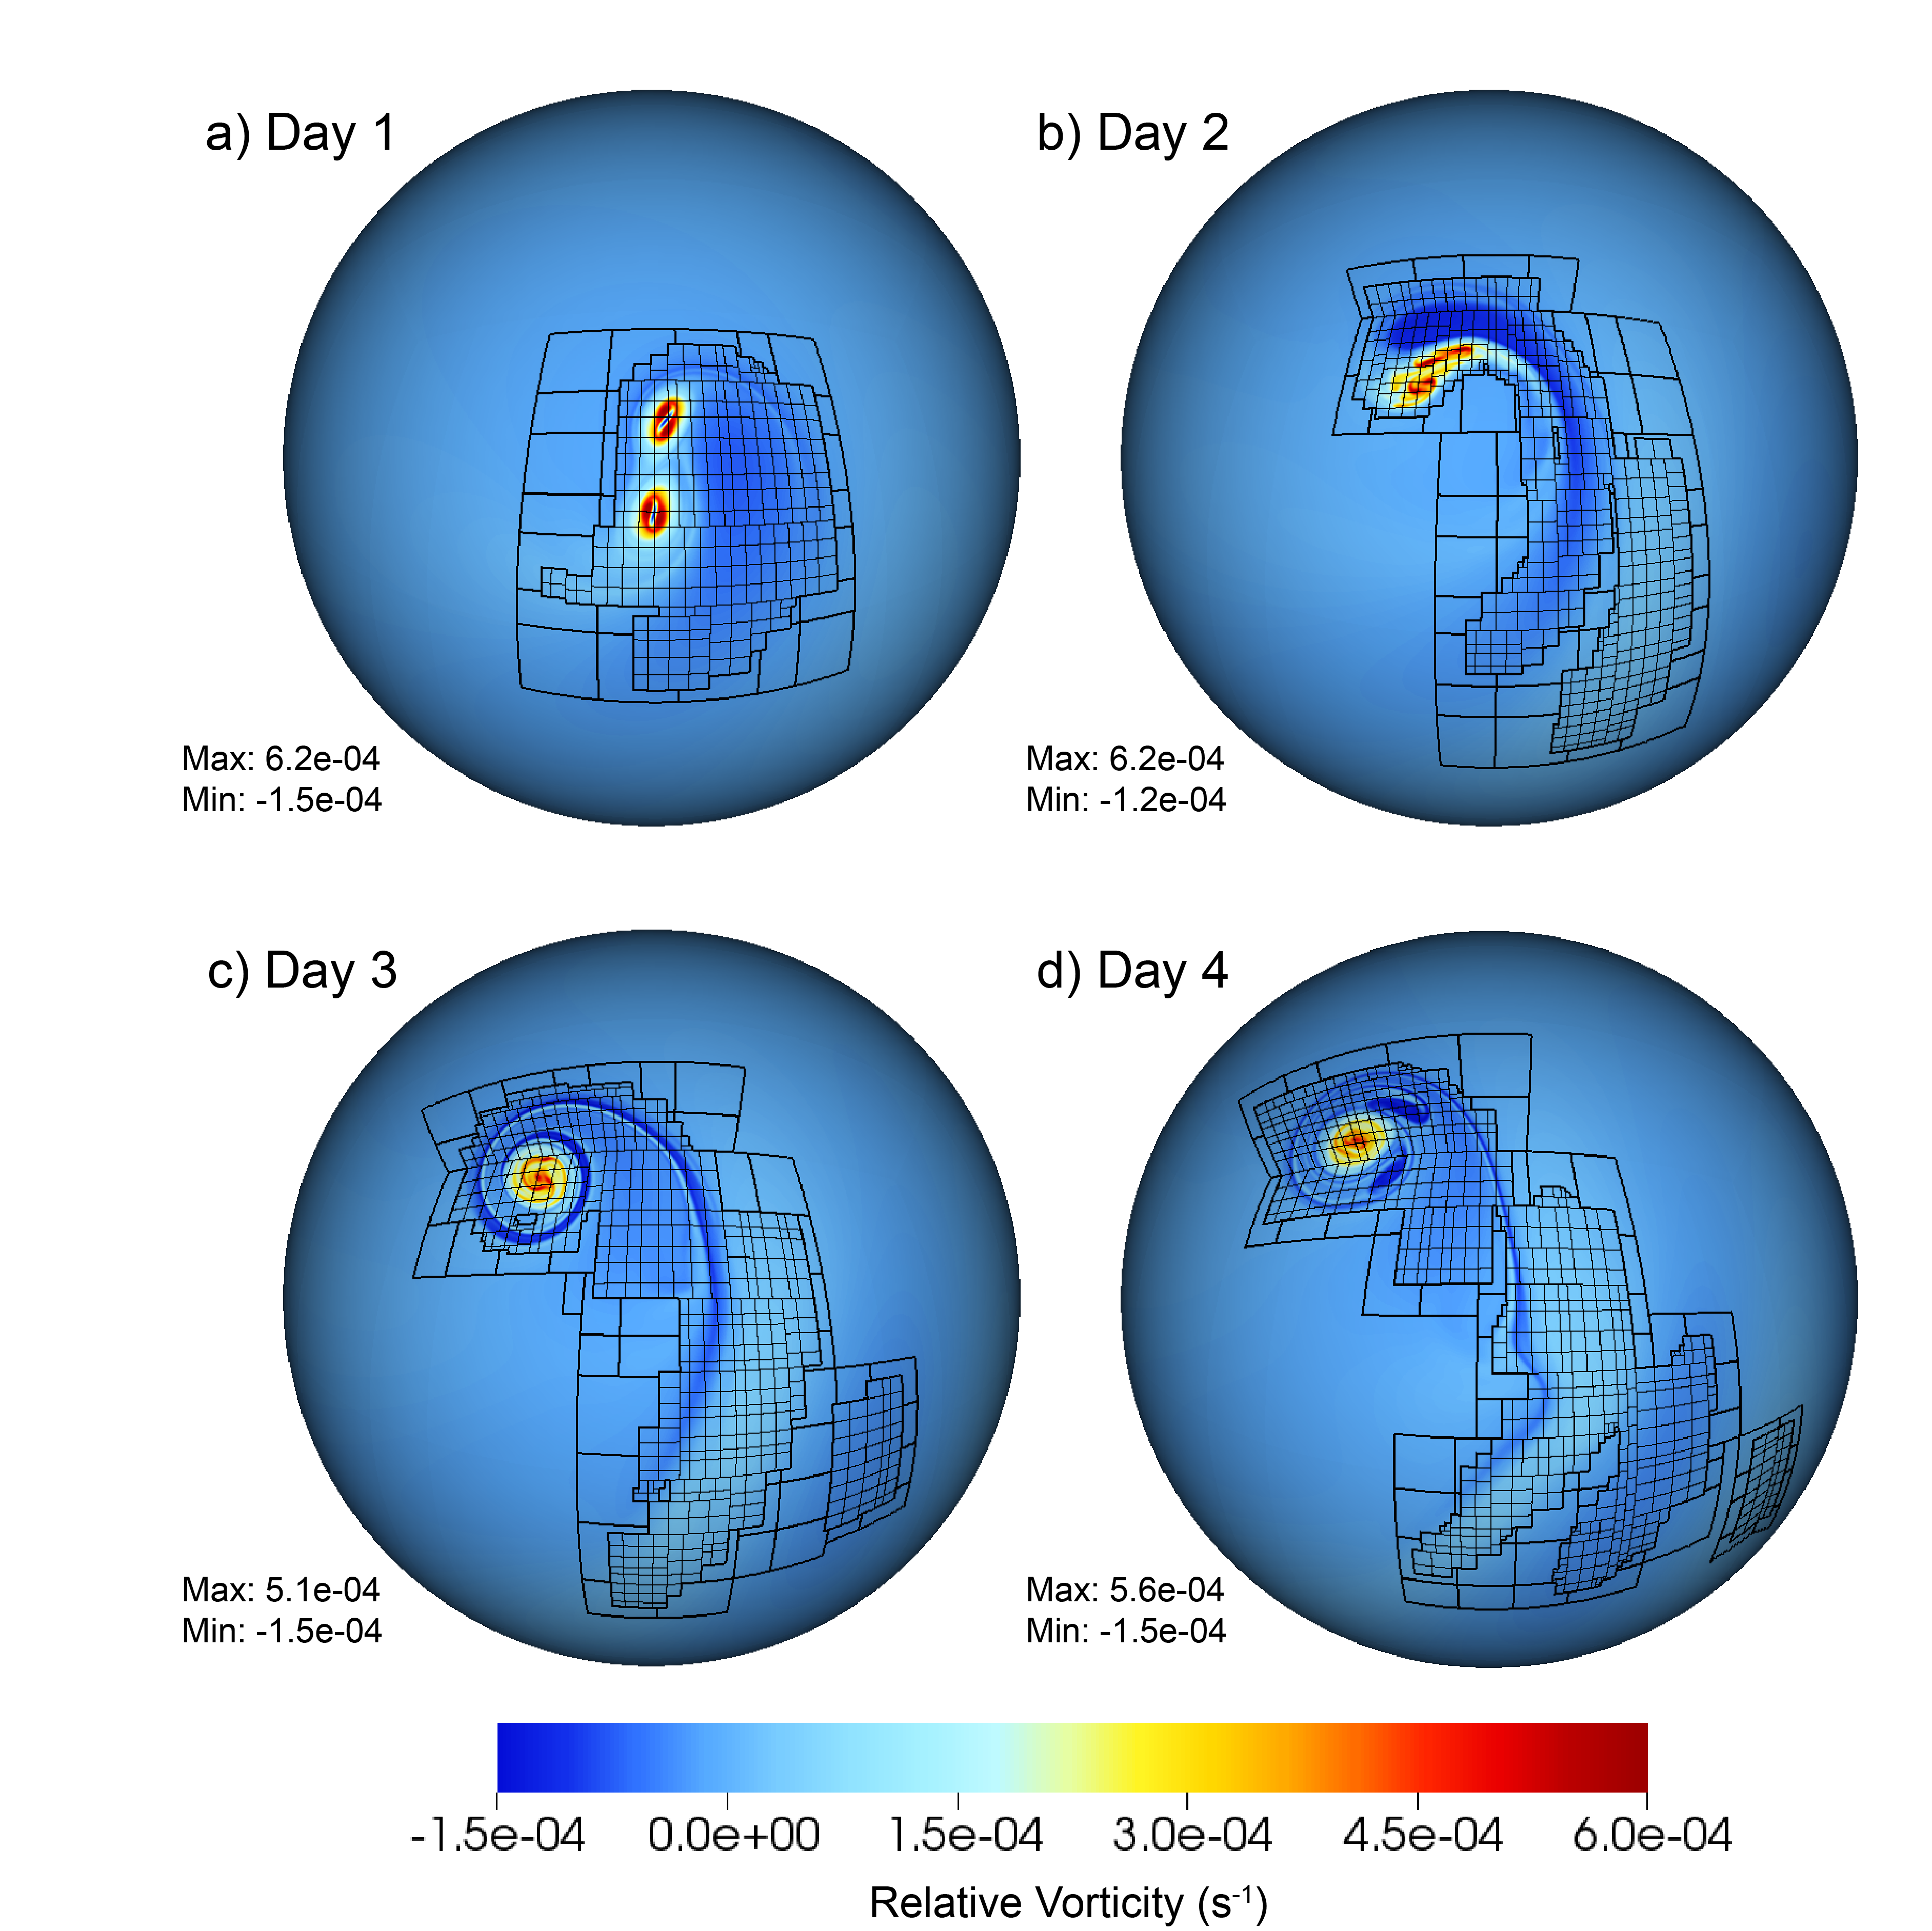
\includegraphics[width=19pc]{Chap1/amr_daysMerge}}
    \caption{Evolution of the merging vortices in the test of 
Section~\ref{subsubsec:merging-vortices}
in a 2-level AMR run (c64/c256/c1024)
    using a relative-vorticity threshold refinement criterion.
    Refinement occurs when the absolute value of the relative vorticity
    is greater than $2.3 \times 10^{-5} \mathrm{ s}^{-1}$.  Snapshots of relative
    vorticity at day (a) 1, (b) 2, (c) 3, and (d) 4 are depicted.
    The block structures of the c256 and c1024 refinement levels are
    indicated by black contours.}%
    \label{fig:amrmerge_evolve}
\end{figure}
%
Figure~\ref{fig:amrmerge_evolve} depicts the evolution of these vortices as
they merge over the course of four simulation days.  As in the previous case,
though small changes in initial condition lead to very different
results, we do observe a slow convergence with increasing resolution.
We ran the test case with several configurations using one and two
levels of AMR with criteria based on a relative vorticity or a height
gradient threshold.  The AMR run shown in 
Fig.~\ref{fig:amrmerge_evolve} has a c64 base resolution with two levels of
x4 refinement so that its finest level has a c1024 resolution.  The AMR
is triggered when the absolute value of the relative vorticity exceeds
$2.3 \times 10^{-5}$ s$^{-1}$.  With that relatively low
refinement threshold, the AMR captures not only the main vortex cores,
but also the small-scale anti-cyclonic filament that extends far south
of the merged vortex, and the small-magnitude wave train that develops by
day 4.  Figure
\ref{fig:merge_amr_comp} shows a column comparison of the vorticity
field at day 4 for uniform-resolution runs and AMR runs using three
refinement criteria.  The first column contains the uniform c1024 run
and three 2-level AMR runs with x4 refinement on c64 base resolution
that have a finest resolution of c1024.  The second column has the c512
uniform run and three 2-level AMR runs with a c32 base.  The last column
has the uniform c256 run and three 2-level AMR runs with a c16 base.
The three AMR refinement criteria in 
Fig.~\ref{fig:merge_amr_comp} are
\begin{itemize}
    \item[1.]
        Large-height-gradient-tag AMR:  tag where the absolute value of
        the height gradient is $|\nabla h| > 4 \times 10^{-4}$ (second
        row of Fig.~\ref{fig:merge_amr_comp})
    \item[2.]
        Small-height-gradient-tag AMR:  tag where 
        $|\nabla h| > 1 \times 10^{-4}$ (third row)
    \item[3.]
        Vorticity-tag AMR:  tag where the absolute value of the relative
        vorticity is $| \zeta | > 3.5 \times 10 ^{-5}$ s$^{-1}$ (fourth
        row)
\end{itemize}
Locally refining the grid resolution with AMR effectively achieves a
similar result in the refined areas as the corresponding high-resolution
uniform runs.  Even the large-height-gradient refinement threshold used
in Figs.~\ref{fig:merge_amr_comp}b and
\ref{fig:merge_amr_comp}f, which results in very little refinement, is
still able to produce a very similar vortex structure and position
within the refined area demonstrating little to no negative effects from
the coarse-fine boundaries surrounding the vortex.  The lower refinement
thresholds are further able to capture the anti-cyclonic filament
wrapping around the new vortex and extending down from it as well as the
development of the secondary lee side wave train. 
%
\begin{figure}
    \centerline{%
    \noindent
    \includegraphics[width=0.75\textwidth]{Chap1/merge_amr.eps}}
    \caption{Relative vorticity field at day 4 on the cubed-sphere grid
    for several runs of the merging-vortices test of
Section~\ref{subsubsec:merging-vortices}
using AMR.  (a) Uniform c1024 run, (e) uniform c512 run, and (i) uniform
    c256 run.  (b), (c), and (d) are AMR runs whose highest refinement
    level is c1024.  (f), (g), (h) AMR runs have a maximum refinement
    level of c512 while (j), (i), and (l) AMR runs have a c256 maximum
    resolution.  (b), (f), and (j) depict AMR runs with two level of
    refinement using the large-height-gradient tag.  (c) , (g), and (k)
    depict 2-level AMR runs using the small-height-gradient tag.  In the
    last row, (d), (h), and (l) the 2-level AMR runs use the
    relative-vorticity tag.  Thus in the first column, all the AMR runs have a
    c64 base grid, a c32 base grid in the second column, and a c16 base
    grid in the third.  All AMR runs use a x4 refinement ratio.}%
    \label{fig:merge_amr_comp}
\end{figure}
%
The convergence to
the error of the uniform-resolution runs can be observed in the normalized $l_2$
vorticity error seen in Fig.~\ref{fig:symvor_merge_l2err}. 
The $l_2$ error norm is computed by
comparing runs to the uniform c1024 run which serves as a reference solution. 
The figure depicts the normalized $l_2$ relative vorticity error 
(Fig.~\ref{fig:symvor_merge_l2err}a) and total number of grid cells 
(Fig.~\ref{fig:symvor_merge_l2err}b) as a function of forecast days for uniform-resolution runs and
1- and 2- level AMR runs using the large-height-gradient tag or the
vorticity tag with x4 refinement ratios. The vorticity-tag AMR
simulations (both 1- and 2-level AMR) have nearly the same error as the
uniform runs with the highest resolution while the gradient-tag runs
have slightly higher error.  This agrees with the fact that the
gradient-tag runs use fewer grid cells and only cover the merged vortex
core (see 
Figs.~\ref{fig:merge_amr_comp}b, f, and j).
Although the large-scale shape and
locations of the two merging vortices and the post-merger vortex appear
visually to converge to a solution with increasing resolution, we do not
observe a large reduction in the global errors with increasing
resolution.  The source of this error is the small differences that
occur in the core of the vortices, caused by small-scale non-linear features
in the high-vorticity filaments, as well as slight variations in the beta
drift created by small changes in the vorticity magnitude for the
different resolution runs.  These small differences in these features
lead to localized large-magnitude errors in the vorticity.  As in the
separation case, the AMR improves the solution using fewer grid cells.
Even when the AMR patch over the vortex is small and the coarse-fine
boundary is near the high vorticity cores, the solution is not
negatively distorted, showing the robustness of the model given the
sensitivity of the test case to grid resolution and slight changes in
initial conditions.

%
\begin{figure}
    \centerline{%
    \noindent
    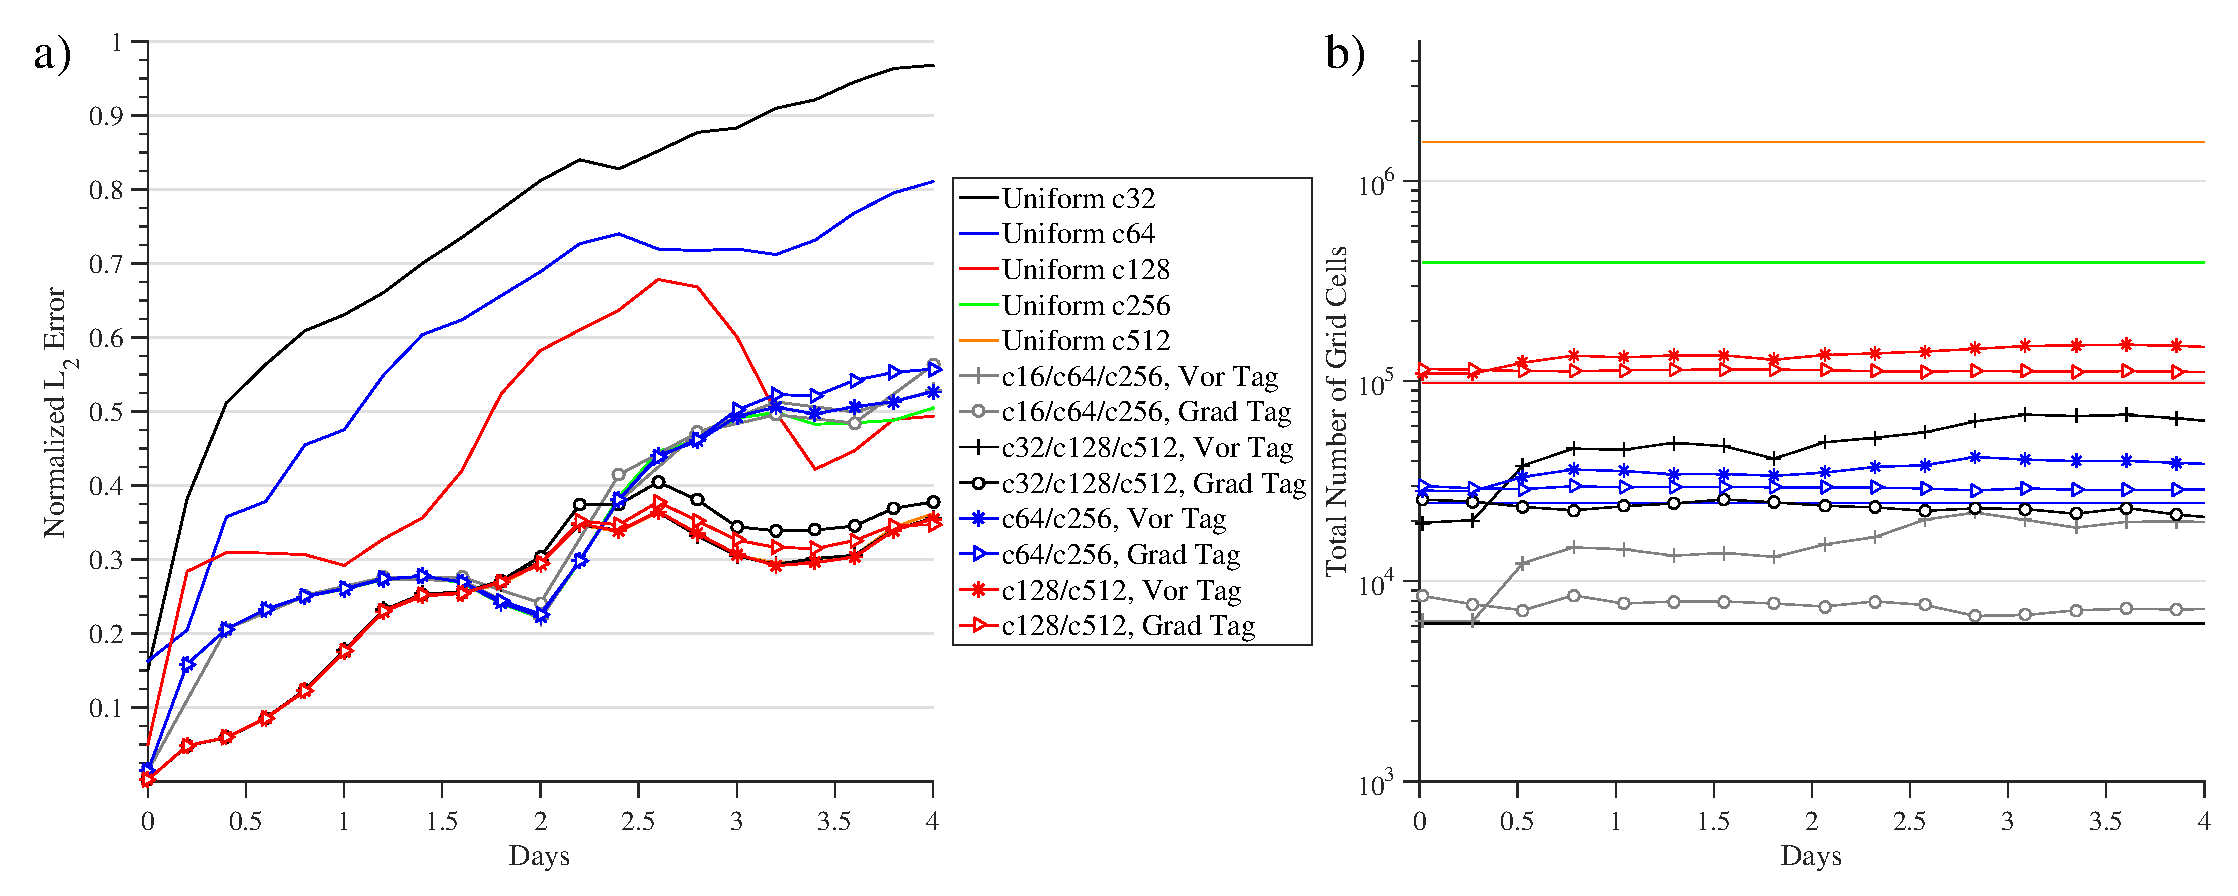
\includegraphics[width=\textwidth]{Chap1/final_symvor_merge_l2err_grid.eps}}
    \caption{
    For the merging-vortices test of
Section~\ref{subsubsec:merging-vortices},
growth over the four-day period of:
(a) normalized $l_2$ error for relative vorticity calculated with respect to the uniform c1024 run, and
 (b) total number of grid cells.
Error and number of grid cells are for uniform runs and 1- and 2-
    level AMR runs using the large-height-gradient tag or the
    relative vorticity tag with x4 refinement ratios.}%
    \label{fig:symvor_merge_l2err}
\end{figure}
%
\begin{table}
    \caption{Run times (wall-clock time in s and as \% of the
    c512 time) for 4-day merging-vortices simulations
(Section~\ref{subsubsec:merging-vortices})
with uniform and AMR runs
    using only eight processors on one node of NCAR's Yellowstone computing platform. The total number of cells is counted at day 4.}%
    \label{tb:mergvor_time}
    \resizebox{\textwidth}{!}{
     \begin{tabular}{lcrrrr}
        \hline
        AMR Res.           & AMR Levels         & Run Time (s)            & Run Time (\%)            & Total cells             & Total cells (\%)        \\ 
        \hline
        \hline
        c512               & -                  & $24127$                 & 100\%                    & $1.6 \times 10^{6}$     & $100\%$                 \\ 
        c128/c512          & 1                  & $1913$                  & 7.9\%                    & $1.9 \times 10^{5}$     & $12\%$                  \\ 
        c32/c128/c512      & 2                  & $1225$                  & 5.0\%                    & $1.2 \times 10^{5}$     & $7.5\%$                 \\ 
        \hline
        c256               & -                  & $3596$                  & 15\%                     & $3.9 \times 10^{5}$     & $25\%$                  \\ 
        c64/c256           & 1                  & $394$                   & 1.6\%                    & $5.5 \times 10^{4}$     & $3.4\%$                 \\ 
        c16/c64/c256       & 2                  & $304$                   & 1.3\%                    & $3.6 \times 10^{4}$     & $2.3\%$                 \\ 
        \hline
        \hline
    \end{tabular}
    }
\end{table}

The computing run times versus number of grid cells for a 4-day simulation with vorticity tagging
is presented in Table \ref{tb:mergvor_time}. The table thereby represents some of the runs from
Fig.~\ref{fig:symvor_merge_l2err}b. Eight processors on one node of NCAR's Yellowstone computing 
platform are used.
We see the approximate $8\times$ reduction in cost between the c512
and c256 uniform runs, as expected for a doubling of the horizontal resolution and a halving of the time step.
For this test, the wall-clock run time for AMR runs
is closer to $\approx 4\times$ for $2\times$resolution changes, 
demonstrating some of the overhead of the AMR algorithm.
The total wall-clock time roughly correlates with the total number 
of grid cells, as in the moving-vortices advection test,
even for the coarsest 2-level AMR runs (c32/c128/c512 and c16/c64/c256).

\section{Conclusion}
\label{sec:conclusion}

In this chapter, we utilized a fourth-order
finite-volume model on a cubed-sphere grid, which is adaptive in both
space and time, to demonstrate the effectiveness of the AMR in resolving
and tracking chosen features of interest while maintaining large-scale
smooth flows.  Using selected shallow-water and advection test cases, we
evaluated the AMR's ability to track and resolve features of interest
without creating distortions or numerical noise in the large-scale
smooth flows at the interfaces between meshes.  A variety of static and
dynamic refinement criteria and strategies are implemented to assess the
strengths and weaknesses of the AMR method.  With the large-scale smooth
``do no harm" tests, one and two levels of static and adaptive
refinement meshes with several refinement ratios were placed at several
locations on the cubed-sphere grid.  The results confirmed that multiple
levels of refinement and abrupt x4 or x8 refinement ratios between
levels still allowed flows to move smoothly through the refined areas.
There was little induced noise and numerical error at the refinement
boundaries.  For coarse resolutions, the refinement improved global
errors slightly, and the errors remained nearly unchanged when refinement
was added to higher-resolution base grid for the two shallow-water
tests.  Only for high resolutions in the USBR tests when a moving AMR
grid transected the cubed-sphere panel boundaries did we see a
noticeable increase in error.  This error, however, was very localized
and only becomes apparent because the base global error is so low in the
uniform resolution simulations for this smooth idealized test.  In the
coarser runs for the USBR and in the other more complex shallow-water
tests with larger expected global errors, this was not observed.

With the three AMR test cases, we demonstrated that AMR is able to track
the features of interest and closely reproduces the results of uniform
high-resolution runs using fewer grid cells.  AMR was implemented using
tracer and height-field gradients as well as relative-vorticity
magnitude
as tagging criteria with multiple refinement levels and
a range of thresholds.  
The AMR grids are added and removed in time without creating significant
distortions or noise at the mesh interfaces.  In the tracer advection
test, fourth-order convergence was maintained while using AMR, and the
error of AMR runs with one level of refinement was comparable to the
error of uniform runs having the same fine-level resolution.  The test
showed the importance of refining early, as errors developed from the
coarse grid propagate through the fine grids for the rest of the
simulation.  The gravity wave impinging on the mountain test
demonstrated the use of AMR with topography.  Refinement was added and
removed from the areas with topography without creating additional
negative impacts.  In the binary-vortices test, AMR improved accuracy of
the position of the vortices as they interacted and their structures
when compared with uniform resolution runs.  Even stringent criteria 
with high threshold values, which did not create a large buffer of high resolution
around the vortices, still produced accurate results and improved the
solution in the refined patches.  Additional refinement, though,
significantly improved the representation of the vorticity filaments
that extended well away from the central vortices and the developing
Rossby wave train.

All three test cases demonstrated that a variety of AMR criteria and
thresholds lead to improvements in the results, though to maximize that
improvement, the refinement criteria needed careful tailoring.  Several
conditions increased the effectiveness of AMR; however, there was no
clear strategy for establishing the best general refinement criteria.
Having initial refinement or refining early in the run before errors
developed on the coarse grid was one of the key strategies for improving
accuracy.  When there is no initial refinement, the benefits of AMR are
limited by the coarseness of the base mesh;  
AMR with two levels was ineffective due to large errors introduced by 
the coarsest base meshes early in the calculation. 
This speaks to the need for a sufficiently-refined base
mesh to avoid contaminating finer levels. 
Using more than one level
of refinement and effective tagging strategies resulted in 
better-resolved features of interest, but at a
diminishing rate of return of improvement. 
Our conclusion is that the
benefit of AMR does not come automatically from the computational 
savings of a very coarse base mesh. However, there may still be benefits 
of two or more levels over uniform-resolution calculations that otherwise 
would not be computationally feasible without AMR.
In a realistic climate simulation,
tropical cyclones could, perhaps, be effectively captured early by
criteria that place high resolution over the cyclogenesis region and then
refine over and track emerging storms to ensure continued accuracy.
For other, more complex or moist flows, more advanced criteria than just
a simple relative-vorticity threshold need to be investigated.  They
could be based, for example, on combinations of physics-based properties (like
rainfall), thresholds of vorticity, or gradients.  Future work will
explore such refinement criteria in the 3D non-hydrostatic version of
the Chombo-AMR model with and without a variety of physical
parameterization schemes.  The addition of physical parameterizations
will also allow us to test the scale awareness of the physics schemes.

 \chapter{Assessing AMR in forced shallow water systems with moisture}
 \label{chap:forcedsw}
 \section{Introduction}
The spherical shallow water equations serve as an effective test bed for 
assessing numerical methods for general circulation models (GCMs). They 
exhibit many of the dynamics and complexities of the full 3D equations with 
the advantage of being two-dimensional and thus less computationally intensive.  
Full 3D models use the dycore of the GCM with
 a plethora of sub-grid parameterization 
schemes for unresolved physical and thermodynamical processes, further 
adding to their complexity.  However, shallow water-type models and 
the unforced test cases traditionally associated with them \citep{Williamson:1992kx}
are missing features (e.g. water vapor, convection, latent heat release, 
thermal forcing) which play key roles in atmospheric and 
climatological phenomena. Including simplified forcing mechanisms to represent 
such moisture and heating
processes in the shallow 
water system narrows the gap between idealized unforced studies 
and full-physics models. These forced shallow water 
models include the dynamical complexities of the full models and can retain
the non-linearity of the physical processes.  However,
the shallow water equations are still simple enough to effectively study
the key components of the dycore such as the numerical algorithms,
computational grid, and, for variable resolution and AMR models, grid refinement
strategies and efficacy. Shallow water models have the added advantage of being
computationally cheap to run at high resolutions.

A variety of studies have implemented forcing in shallow water models to study
 the fundamental dynamical aspects of large synoptic
scale climatological features, such as the Madden-Julian Oscillation (MJO),
as well as intense, small-scale features including tropical cyclone 
evolution, cumulus convection, and frontal propagation.
\cite{ferreira1996dynamical} and \cite{yang2013triggered} implement
spatially and temporally varying mass sinks and sources within nonlinear 
shallow-water models to simulate MJO convection in studies of MJO
induced twin tropical cyclones and MJO convective envelope 
development, respectively. In \cite{enagonio2001tropical}, 
the authors examined tropical cyclogenesis
by forcing a shallow water system with periodic pulses of vorticity to represent multi-burst convection.
 \cite{hendricks2014hurricane} mimicked diabatic heating in hurricane 
eyewalls within a Cartesian shallow water model by using a prescribed annular
 axisymmetric mass sink.

A framework to study the specific dynamical role of moist processes in a shallow water system
was proposed in the seminal work by \cite{gill1982studies}. In this system,
 a moisture equation with nonlinear precipitation thresholds was added to the 
linearized shallow-water equations to model the effects of latent heat release on the 
propagation of large scale disturbances. Similar models incorporating this framework for 
parameterizing moisture were analyzed by \cite{goswami1991modification} in the context of
large-scale equatorial wave propagation and by \cite{frierson2004large},
\cite{stechmann2006structure}, and \cite{bouchut2009fronts} in studies of tropical precipitation 
fronts. Unlike the other studies mentioned, \cite{bouchut2009fronts} implements the moist-convective 
parameterizations in a fully nonlinear rotating shallow water model,
also used by \cite{lambaerts2011moist} to compare the differences in barotropic instability evolution between moist and dry conditions. To study the
dynamical role of moisture in tropical cyclone instabilities, \cite{lahaye2016understanding} 
also used this moist rotating shallow-water model with an added evaporation 
mechanism. \cite{rostami2017influence} implemented both a 1-level barotropic 
version and a 2-level shallow water baroclinic version of the model introduced in 
\cite{lambaerts2011moist} to study large-scale small Rossby number vortices.

Other frameworks for simulating precipitation and convection in the shallow water
system that have been implemented recently included models by 
\cite{wursch2014simple} and \cite{zerroukat2015moist}.
\cite{wursch2014simple} developed a simplified model of cumulus convection 
incorporating representation of updrafts, downdrafts, and idealized precipitation 
effects in a 1D shallow water model. 
Once the fluid exceeds a certain threshold height, signaling the 
onset of convection, mechanisms serving as simplified representations 
of cumulus convection modify the geopotential height to create
conditional instability and mimic updrafts. 
This method was extended to a rotating, 2D shallow 
water model in \cite{kent2017dynamics}.
In \cite{zerroukat2015moist}, the authors re-derived the two-dimensional
shallow water system from the three-dimensional moist Boussinesq 
approximation. Density was permitted to vary with temperature,
resulting in additional buoyancy related terms in the momentum equations and
permitting a dynamics-moisture feedback. \cite{zerroukat2015moist} also 
implemented a three-state moisture model consisting of vapor, cloud, and 
precipitated species.

In this paper, we implement two forcing frameworks that seek to mimic moisture 
and convection in a spherical, 2D shallow water system. In the first, 
 moist shallow water equations derived in \cite{bouchut2009fronts} and 
\cite{lahaye2016understanding} cause
 convective forcing and precipitation, which induce TC-like vortices to develop and strengthen. In the second 
framework, the barotropic instability shallow water test case of 
\cite{galewsky2004initial} is implemented within a different moist shallow water system developed from 
 \cite{zerroukat2015moist}. As the jet becomes unstable and collapses, front-like 
 systems containing clouds and precipitation develop. Using these frameworks, we
 investigate the distinctive dynamics produced by the non-linear physics processes
 within the traditional shallow water system. A main goal of this paper is to
 introduce test cases with more challenging complex and transient features
 to test the ability of adaptive mesh refinement (AMR) 
 to track and resolve these moving and growing features.
 
 We use the fourth-order finite-volume Chombo AMR model
 presented in \cite{mccorquodale2015adaptive} and
 \cite{ferguson2016analyzing} for the 2D shallow water equations. 
 This model implements dynamic refinement using
 a mapped-multiblock AMR technique which overlays the base grid with more refined patches.
 Using AMR, we observe how features in the test cases evolve due to the forcing 
 processes and how those forcing processes are affected by the AMR refinement. 
Ideally, the physics forcing schemes should be able to effectively span 
the multiple levels of refinement and changing resolutions created by AMR.
 In addition, we seek to quantify improvements gained from AMR grids
 and determine effective refinement criteria.

This chapter is organized as follows. Section \ref{sec:modelintro} provides a brief overview
of the finite volume model and the Chombo multiblock AMR techniques.
Section \ref{sec:forcedvort} describes the shallow water equations
with moist convective forcing and the strengthening vortex test case.
Section \ref{sec:wetvortresults} compares numerical results of the strengthening vortex
test case for uniform and AMR runs of varying resolution. The
 \cite{zerroukat2015moist} moist shallow water system with
 barotropic instability test case and its numerical results
 are presented in Section \ref{sec:kesslersw}.  Section \ref{sec:conclusion2} summarizes our
 conclusions from the two test cases.

\section{High-Order Finite-Volume Chombo AMR Model}
\label{sec:modelintro} 
  For this study we employ an unstaggered finite-volume (FV) mapped-multiblock 
  dynamical core (dycore) that is fourth-order accurate and adaptive in both 
  space and time. The model's AMR is based on the Chombo AMR 
  library \citep{Adams:2015gd} and an in-depth description of the model 
  dynamical core for the shallow-water equations on an equiangular cubed-sphere 
  grid can be found in \cite{mccorquodale2015adaptive}. The model is mass 
  conserving and conserves energy up to the temporal truncation error, when 
  limiters or explicit dissipation are not applied. 
  
  The cubed-sphere grid consists of a cube whose six separate panels are 
  projected onto the surface of a sphere. In addition to eliminating the polar 
  singularities found in spherical latitude-longitude grids, the equiangular cubed-sphere 
  also leads to a quasi-uniform mesh with similarly sized grid cells across the sphere. 
  The discrete resolution of the cubed-sphere grid is denoted by $c\{N_c\}$ 
  where $N_c$ is the number of grid cells in each direction on a panel. Several 
  properties of the equiangular cubed-sphere grid, including approximate grid 
  spacings, are given in Table~\ref{tb:grids2} for resolutions used in this chapter. 

\begin{table}[t]
    \caption{Properties for several cubed-sphere grid resolutions where 
    $N_c$ is the number of cells along an edge of a cubed-sphere panel.
    Here the number of cells is the total number of grid cells 
    ($N_c^2 \times 6$), $\Delta x$ is the approximate grid spacing, 
    $A_{avg}$ is the average area of a grid cell, $A_{min}/A_{max}$ is the
    ratio between the minimum and maximum cell areas, Eq.  Res.  is the
    grid resolution in degrees given by $90^\circ / N_c$, and $RLL_{equiv}$
    is the equivalent grid spacing on a regular latitude-longitude
    grid with the same total number of cells.}%
    \label{tb:grids2}
    \begin{center}
    \resizebox{\textwidth}{!}{
    \begin{tabular}{cccrccc}
            \hline
            Resolution ($N_c$) & No. of cells       & $\Delta x$ (km) & $A_{avg} (\mbox{ km}^2)$ & $A_{min}/A_{max}$ & Eq. Res.     & $RLL_{equiv}$ \\ 
            \hline
            \hline
            c$32$              & $6.14 \times 10^3$ & $313$           & $8.302 \times 10^{4}$    & $0.7249$          & $2.81^\circ$ & $3.25^\circ$  \\ 
            c$64$              & $2.46 \times 10^4$ & $156$           & $2.076 \times 10^{4}$    & $0.7159$          & $1.41^\circ$ & $1.62^\circ$  \\ 
            c$128$             & $9.83 \times 10^4$ & $78.2$          & $5.189 \times 10^{3}$    & $0.7115$          & $0.70^\circ$ & $0.82^\circ$  \\ 
            c$256$             & $3.93 \times 10^5$ & $39.1$          & $1.297 \times 10^{3}$    & $0.7093$          & $0.35^\circ$ & $0.41^\circ$  \\ 
            c$512$             & $1.57 \times 10^6$ & $19.5$          & $3.243 \times 10^{2}$    & $0.7082$          & $0.18^\circ$ & $0.20^\circ$  \\ 
            c$1024$           & $6.29 \times 10^6$ & $9.77$          & $8.107 \times 10^{1}$    & $0.7076$          & $0.09^\circ$ & $0.10^\circ$  \\ 
            c$2048$           & $2.52 \times 10^7$ & $4.89$          & $2.027 \times 10^{1}$   & $0.7074$          & $0.04^\circ$ & $0.05^\circ$ \\
            \hline
        \end{tabular}
        }
    \end{center}
\end{table}
 
  The model uses a classical fourth-order Runge-Kutta (RK4) 
  time discretization scheme. in the spatial domain, fourth-order 
  accurate finite-volume discretization is implemented to compute 
  flux averages on the faces of each cell. In addition, a high-order 
  least-squares interpolation is used to compute stencil operations near panel 
  or block boundaries. The stencil operations create three layers of ghost cells 
  at the panel edges to preserve the order of accuracy of the fluxes. 
  At a panel edge, the fluxes for cell faces along the panel edge are calculated 
  separately for each panel and are then averaged together. This mean value 
  is taken as the flux for each face to ensure conservation. Additionally, a sixth-order 
  diffusive operator is applied to smooth the flux calculations while still 
  maintaining the scheme's fourth-order accuracy. 
  
  Our mapped-multiblock AMR approach implements a hierarchy of 
  nested grid levels of increasing resolution, using the numerical tools 
  developed in the Chombo AMR library \citep{Adams:2015gd}. 
  The grid resolution of an AMR level is defined by its refinement ratio 
  to the grid resolution of the coarser level below it. Finer levels are 
  placed over regions where coarse cells have been marked (tagged) 
  by the model as meeting the refinement criterion. The cell values in 
  the finer level are initialized via interpolations from the coarser level. 
  Ghost cells are used to calculate fluxes at the level boundaries in the 
  same manner as is done at the cubed-sphere panel boundaries. If 
  multiple levels are used, intermediate levels must cover enough area 
  to ensure that the finer level is nested within the intermediate level; it 
  is required that the ghost cells for the finer level are only interpolated 
  from cells within the intermediate level.  
  
  Finer levels are sub-cycled in time to maintain a constant Courant 
  number across all resolutions. The sub-cycling routine can be 
  summarized as follows: after interpolating values to the refined 
  level, the coarser level is advanced by one time step. The finer level 
  is then advanced in time using a smaller time step determined by 
  dividing the coarse time step by the refinement ratio between the two 
  levels.  At each finer time step, the ghost cells used to calculate the 
  boundary fluxes at the finer level's edges are updated via a temporal 
  interpolation from the RK4 method. After the sub-cycling is complete, 
  the values on the coarse grid are updated from the solution on the 
  finer grid.  \cite{mccorquodale2015adaptive} and \cite{ferguson2016analyzing} 
  both provide more detailed descriptions of the AMR technique. 
  
  The refinement criteria determine the regions over which additional 
  grid levels are placed based on user-selected threshold values for 
  flow properties.  The thresholds are set independently for each 
  simulation and their criteria can be based on a variety of properties, 
  such as tracer values, gradients, relative vorticity, or a combination of 
  these. The AMR dycore can incorporate multiple levels of refinement, 
  preset for each simulation, and tagging criteria can be uniformly 
  enforced across all levels or required to scale with increasing resolution.
 
%--------Section 
\section{Convectively forced shallow water vortices}
\label{sec:forcedvort} 
  This test cases simulates the growth and development of TC-like 
  vortices in a 2D shallow water framework using a moist convective forcing 
  mechanism. Weak vortices are initialized on a calm background field 
  of uniform height. Evaporation and precipitation cause these vortices to strengthen. 
  After several days of strengthening, the orderly vortices collapse and a more chaotic 
  system evolves, characterized by several smaller vortices and jet-like background flow. 

  We first provide a description of the moist convective shallow water system 
  and an overview of the initial conditions. Next we present the evolution of an 
  isolated vortex in this test case at a uniform high resolution. Then we demonstrate
  the use of AMR in this test case comparing the affects of different resolutions and
  various tagging criteria.

%Subsection
  \subsection{``Moist-convective`` shallow water equations }
     The shallow water equations are modified to include the transport of a 
     moisture variable and the effects of moist convection, precipitation, and evaporation. 
     We extend the forcing schemes developed by \cite{bouchut2009fronts} and 
     \cite{lahaye2016understanding} to the 2D shallow water equations on the sphere. 
     \cite{bouchut2009fronts} developed a moist convective scheme 
     for a rotating shallow water model to study precipitation fronts. 
     It only included an advected moisture variable, precipitation, and 
     a convection mimicking process, while \cite{lahaye2016understanding} 
     added an evaporation forcing to the system.  
     
     In this moist convective system, a relaxation sink is added to the moisture equation (Eq. \ref{eq:swqcon}), 
     representing precipitation when moisture levels exceed a saturation value. 
     A corresponding convective mass sink is added to the continuity equations and a 
     moisture source is added to the moisture equation to represent evaporation. 
     The equations for this modified shallow water system are
   \begin{equation}
     \label{eq:swmomf} \frac{\partial h \mathbf{v}}{\partial t} +
     \nabla \cdot ( h \mathbf{v} \mathbf{v}) + f \mathbf{\hat{k}}\times(h\mathbf{v}) + gh\nabla H = 0
   \end{equation}
   \begin{equation}
     \label{eq:swconf}  \frac{\partial h}{\partial t} + \nabla \cdot (h\mathbf{v}) = - \beta P 
   \end{equation}
   \begin{equation}
     \label{eq:swqcon}  \frac{\partial hQ}{\partial t} + \nabla \cdot (hQ\mathbf{v}) = h(E - P).
   \end{equation}
   Here $\mathbf{v}$ is the velocity vector, $\mathbf{v}\mathbf{v}$ denotes the outer product
   of the velocity vector, $f$ is the Coriolis parameter, $g$ is 
   the acceleration due to gravity,
   $h$ is the height of the fluid, $H$ is the total height including topography, and the
   dimensionless moisture variable $Q$ represents bulk humidity. 
   $E$ is the evaporation in the moisture budget and $P$ is the precipitation. 
   The latent heat release from precipitation does not directly influence the 
   horizontal momentum. It is instead linked to convective vertical velocity 
   directly proportional to $P$ at the upper surface of the fluid.
   Since this system is designed to represent only the lower part of the 
   troposphere, the convective updraft can be constructed as a mass exchange 
   from this surface layer. The mass exchange is then represented as a mass 
   sink in Equation \ref{eq:swconf} governed by an adjustable
   constant $\beta$.  A detailed explanation for the implementation is 
   presented by \cite{bouchut2009fronts}.

   The precipitation sink is calculated in terms of $Q$ and the saturation value $Q_s$,
   \begin{equation}
     \label{eq:precip} P = \frac{Q-Q_s}{\tau}\mathbf{H}(Q-Q_s).
   \end{equation}
   with a relaxation time of $\tau$. $\mathbf{H}(\cdot)$ is the Heaviside function
    so that $P = 0$ whenever $Q \leq Q_s$.
   A common parameterization used in \cite{lahaye2016understanding} is modified
   to include an upper velocity limit on the evaporation rate, thus the evaporation rate $E_r$ becomes
   %\begin{equation}
     \begin{align}
        \label{eq:evap} 
     &E_r  =   \alpha_e  \lvert \vec{v} \rvert & \mathrm{for} \ \lvert \vec{v} \rvert < v_\mathrm{max} \nonumber \\
     &E_r  =   \alpha_e (v_\mathrm{max}) &  \mathrm{for} \ \lvert \vec{v} \rvert > v_\mathrm{max} 
     \end{align}
   %\end{equation} 
   where the evaporated moisture is dependent on the magnitude of the 
   velocity $\vec{v}$ and the adjustable coefficient $a_e$. This evaporation scales 
   with wind speed until $v_{\mathrm{max}}$. In the simulations presented below,
   $a_e = 0.055$ m$^{-1}$ and $v_{\mathrm{max}} = 30$ m s$^{-1}$.
   At higher velocity magnitudes, $E_r$ is constant.
   
   As established, evaporation is unlimited, but such a setup can lead to runaway 
   supersaturation and very large height forcing which causes exceedingly high wind 
   velocities and negative height values in longer simulations.
   To limit these sources of instability, we refine the forcing mechanics with the following additional mechanisms.
   We add a moisture reservoir from which the evaporation is drawn. This reservoir is a simplistic representation of
   ocean surface heat content and its limiting effects on tropical convection and tropical cyclone intensity.
   In this forcing scheme, the evaporation rate $E_r$ defined in Eq. \ref{eq:evap} draws moisture from the finite reservoir 
    $C_r(\phi,\lambda)$. However, evaporation cannot exceed the amount
    of moisture remaining in $C_R$ for any given latitude-longitude $(\phi,\lambda)$ point in space and time.
    Thus, the evaporation rate $E$ applied in Eq. \ref{eq:swqcon} is capped so that
    \begin{equation}
      \label{eq:crlimit}
         E = \frac{1}{\Delta t}\min\left(E_r \Delta t, C_r\right)
    \end{equation}
   where $\Delta t$ is the model time step. So the evaporation 
   rate becomes zero if there is no longer moisture to be drawn from $C_r$.
    
    The amount of moisture in the reservoir is affected by
    evaporation which removes moisture from 
    the reservoir, and a Newtonian relaxation slowly returns the reservoir to its initial state. 
    The rate of change of moisture in the reservoir is
    \begin{equation}
        \label{eq:ocean} 
        \frac{\partial C_r(\phi,\lambda)}{\partial t} = - E + \frac{1}{\tau_c}(C_0(\phi,\lambda) - C_r(\phi,\lambda))
    \end{equation}
    where $C_0(\phi,\lambda)$ is the initial value and $\tau_c = 10$ days 
    is the relaxation parameter. The initial moisture value $C_0$
    is a zonally symmetric field where
   \begin{equation}
     \label{eq:s0} C_0 = C_{max} \cos^4(\phi)
   \end{equation}
   with the constant $C_{max}= 0.05$. The reservoir is largest near the equator and 
   declines to zero at the poles.  The evaporation rate $E$ as calculated in Eq. \ref{eq:crlimit} 
   ensures that $C_r$ will not go negative.
   
    \cite{bouchut2009fronts} and \cite{lahaye2016understanding} implement a constant 
    $\beta$ to represent the precipitation mass sink. We implement a variable $\beta$ which scales with
    fluid height. As the fluid height decreases below the initial value, $\beta$ is 
    minimized, reducing precipitation forcing and even removing it completely after $h$ has fallen below a certain height. 
    This setup prevents negative fluid height caused by the convective forcing
    and limits the vortex strength.
    Thus the coefficient $\beta$ is set as 
  \begin{equation}
    \label{eq:beta} 
    \beta = \beta_0 \tanh\left(\max\left[0, \lambda_b \frac{h - h_t}{h_0 - h_t}\right]\right).
  \end{equation}
   The constants $\beta_0$ and $\lambda_b$ are set for the tests below to $0.01$ and $10.0$ respectively, 
   while $h_0$ is the initial background height and $h_t$ is the cutoff height set to $75\%$ of $h_0$.
   As implemented in the vortices test case, the $\beta$ term does not limit the vortex strengthening
   until the vortex is well established.

%Subsection
 \subsection{Initialization of vortices}
  The initial conditions of this test case consist of
  one or more weak vortices seeded onto a constant height zero velocity background.
  In the moisture field, each small vortex is initialized with some supersaturation
  to ensure the convective forcing is triggered immediately, creating convergence 
  and allowing the vortices to strengthen.
  
  Each small initial vortex is a small Gaussian depression
  in the uniform height field such that the height field for one initial vortex is
  \begin{equation}
    \label{eq:hforce} h = h_0 - h_{f} \exp{\left(-\left(\frac{r}
    {r_w}\right)^2\right)}.
  \end{equation}
 Here, $h_0 = 4000 \mathrm{ m}$ is the uniform initial height, $h_f$ is the depth 
 of the Gaussian depression, and $r_w$ 
 is the radius of maximum winds. The values for $h_f$ and $r_w$ are designated later for each initial vortex.
 The great circle distance $r$ from
 point $(\phi, \lambda)$ to the vortex center $(\phi_d, \lambda_d)$ is given by ,  and  such that
  \begin{equation}
    \label{eq:gcd} r = a \arccos \left(\sin\phi_d \sin\phi + \cos\phi_d
    \cos\phi \cos\left(\lambda - \lambda_d\right)\right)
  \end{equation}
  with the Earth's mean radius $a = 6.37122 \times 10^6$ m.  The
  chosen $(\phi_d, \lambda_d)$ vortex center points are explained later.
  The corresponding perturbations in the zonal $u$ and meridional $v$ wind  
  components for each vortex are derived from the geostrophic 
  wind balance so that
  \begin{equation}
     \label{eq:uforce} u = -\frac{g}{af}\frac{\partial h}{\partial \phi} 
     = \frac{2 g h_f}{a r_w^2 f} r \exp{\left(-\left(\frac{r}{r_w}\right)^2\right)}
     \frac{\partial r}{\partial \phi}
   \end{equation}
  \begin{equation}
     \label{eq:vforce} v = \frac{g}{af\cos\phi}\frac{\partial h}{\partial \lambda}
     = \frac{-2 g h_f}{a r_w^2 f \cos\phi} r \exp{\left(-\left(\frac{r}{r_w}\right)^2\right)}
     \frac{\partial r}{\partial \lambda}.
   \end{equation}
  The Coriolis parameter $f = 2 \Omega \sin \phi$ has the constant rotation rate
  $\Omega = 7.292 \times 10^{-5}$ s$^{-1}$. The partial derivatives of the great circle 
  distance with respect to spherical coordinates $\phi$ and $\lambda$ are
  \begin{equation} 
  	 \frac{\partial r}{\partial \phi} = \frac{\sin\phi_d\cos\phi - \cos\phi_d\sin\phi\cos\left(\lambda - \lambda_d\right)}
	 {\sqrt{1 - \left(\sin\phi_d \sin\phi + \cos\phi_d\cos\phi\cos\left(\lambda-\lambda_d\right)\right)^2}}
  \end{equation}
  and
  \begin{equation}
  	\frac{\partial r}{\partial \lambda} = \frac{\cos\phi_c\cos\phi\sin\left(\lambda_d - \lambda\right)}
	{\sqrt{1 - \left(\sin\phi_d \sin\phi + \cos\phi_d\cos\phi\cos\left(\lambda-\lambda_d\right)\right)^2}}.
  \end{equation}
  This initialization of the weak vortices is not perfectly balanced on the sphere and 
  will cause the creation of some gravity waves. However, there is no need to further balance
  these initial conditions due to the effects of convective forcing 
  triggered immediately by the initial supersaturation.
  The associated mass sink in Equation \ref{eq:swconf} creates significantly larger gravity waves
   which quickly overwhelm the affects of the initial field imbalances. 
  
  The initial dimensionless moisture profile $Q$ consists of a background profile $Q_0$ and a 
  Gaussian hill leading to supersaturation overlaying each vortex. 
  The background profile has a minimum value at the poles and increases to a 
  maximum just below the saturation point in the equatorial region, and is given by
   \begin{equation}
    \label{eq:q0} Q_0 = \min(Q_{sat} - Q_{off}, \cos\phi + Q_{min})
  \end{equation}
  with the saturation value $Q_{sat}=0.9$, $Q_{off}= 0.01$ sets the maximum 
  background field just below saturation, and $Q_{min} = 0.05$ is the minimum initial moisture
  value at the poles. On top of the background profile is a Gaussian hill which raises the initial moisture
  level in each vortex above saturation. With this perturbation,
   the total initial moisture profile is
   \begin{equation}
    \label{eq:q} Q = Q_0 + Q_{f}\exp{\left(-\left(\frac{r}
    {r_w}\right)^2\right)}
   \end{equation} 
   where $Q_f$ is the maximum moisture perturbation value at the center of the vortex.
   This value is stated later for the individual vortices.
   The initial supersaturation allows the vortex to begin strengthening immediately. It 
   provides the initial convergence which pulls additional moisture toward the vortex center, sustaining 
   the growth of the vortex.  Without supersaturation, the growth of the vortex is less consistent
   and requires more time to initiate. For runs with more than one vortex, 
   the height, velocity, and moisture perturbations for all initial the vortices are summed up 
   and overlaid on the background fields. If the vortices are close together, 
   their fields may significantly overlap.
     
   \subsection{Evolution of a strengthening vortex}
   As a demonstration of the convective forcing mechanisms, we implement the test 
   case by initializing one isolated vortex at a uniform high resolution and observe
   its evolution over twelve days.
   This c2048 resolution ($\sim 5$ km) run serves as a reference solution 
   for AMR and coarser resolution runs. The initial weak vortex is centered at
   $(\phi_d =10^\circ ,  \lambda_d = 0^\circ)$ with maximum height perturbation $h_f=10$ m,
   radius of maximum wind $r_w= 600$ km, and maximum moisture perturbation
   $Q_f=0.0175$. These values result in an initial wind magnitude peak of $ 5.7$ m s$^{-1}$ and 
   a peak moisture value of 0.83\% above the saturation value $Q_s$. The initial vorticity 
   profile is depicted in Fig. \ref{fig:c2048_vortseries}a. In addition, we initialize 
   a non-symmetric binary pair of vortices $90^\circ$ east of the isolated vortex. These vortices 
   interact with each other as they strengthen but do not merge. Each has the same size 
   and strength as the first vortex and but a lower level of supersaturation. 
    The second vortex is centered at
   $(\phi_d =10^\circ , \lambda_d = 90^\circ)$ with $Q_f=0.015$ and the third is
   at $(10^\circ , 105^\circ)$ with $Q_f=0.0125$.
   The two additional vortices have little effect on the 
   evolution of the isolated main vortex during the first twelve days of simulation. They are added
   to the test case to help form a complex chaotic global flow approximately 14 days into the simulation. 
   This analysis and discussion is focused on the single 
   isolated vortex during the initial twelve days; the extended-time (up to 16 days) 
   results focusing on all three vortices are discussed in detail
   in Section \ref{sec:extended}. 
   
\begin{figure}
    \centerline{%
    \noindent
    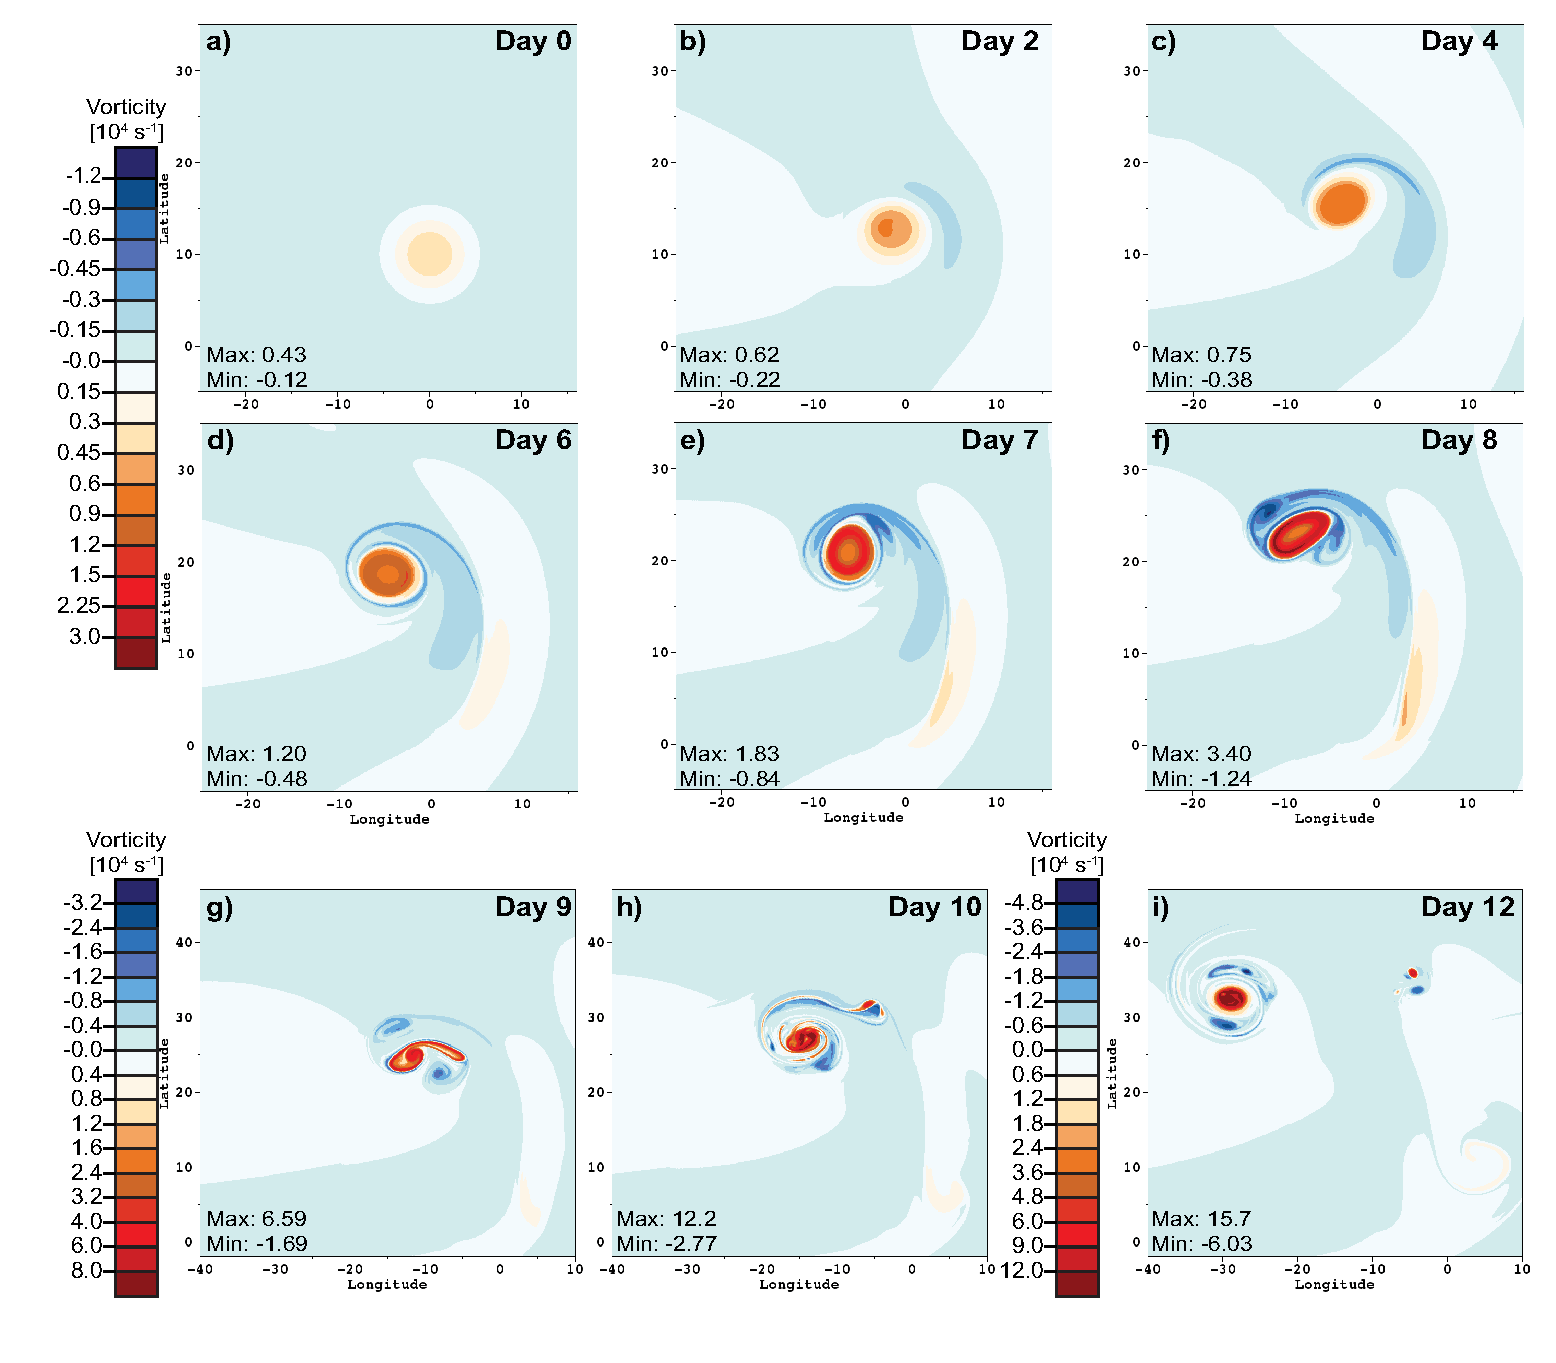
\includegraphics[width=\textwidth]{Chap2/c2048_vort_intime-01.eps}}
   \caption{The evolution of the relative vorticity for an isolated strengthening vortex in a c2048 uniform run.
   (a)-(f) Relative vorticity plots for the initial condition, day 0, and days 2, 4, 6, 7, and 8 with color contour
   range of $-1.2 \times 10^{-4}$ s$^{-1}$ to $3.0 \times 10^{-4}$ s$^{-1}$. (g) and (h) Relative 
   vorticity for days 9 and 10 with the color contour ranged increased to between 
   $-3.2 \times 10^{-4}$ s$^{-1}$ to $8.0 \times 10^{-4}$ s$^{-1}$. (i) Relative vorticity for
   day 12 with a contour range of $-4.8 \times 10^{-4}$ s$^{-1}$ to $12.0 \times 10^{-4}$ s$^{-1}$.
   Note that (g)-(i) have an expanded latitude-longitude domain.}%
    \label{fig:c2048_vortseries}
\end{figure}

    Initial supersaturation triggers convection immediately, 
    creating convergence at the vortex center and driving vortex strengthening.
   The evolution of the vortex's relative vorticity
   profile over a period of twelve days is depicted in Fig. \ref{fig:c2048_vortseries}.
   As the vortex drifts toward the northwest due to beta drift, 
   it undergoes a steady increase in strength over the first six days. 
   At day 6, the maximum wind magnitude has increased to $16.7$ m s$^{-1}$ and the vortex 
   strengthens more rapidly from this point. By the eighth day of the simulation the maximum winds 
   are $31.2$ m s$^{-1}$ and by day 10 they are $69.0$ m s$^{-1}$. 
   
   A key feature that 
   develops around day 4 is a symmetric ring of maximum vorticity. This ring can be clearly 
   seen at days 6, 7, and 8 (Figs. \ref{fig:c2048_vortseries}d-f). As the vortex intensifies more rapidly, this symmetric ring becomes elongated, as
   seen at day 8 in Fig. \ref{fig:c2048_vortseries}f. The unstable elongated ring 
   collapses and the filaments of large positive vorticity begin to collate,
   creating a concentrated area of maximum vorticity (day 9, Fig. \ref{fig:c2048_vortseries}g). 
   A small section of the vorticity filament is not reincorporated into the center spirals
   of the main vortex (day 10, Fig. \ref{fig:c2048_vortseries}h), becoming a separate,
   smaller secondary vortex with a vorticity dipole feature by 
   day 12 (Fig. \ref{fig:c2048_vortseries}i).

\begin{figure}
    \centerline{%
    \noindent
    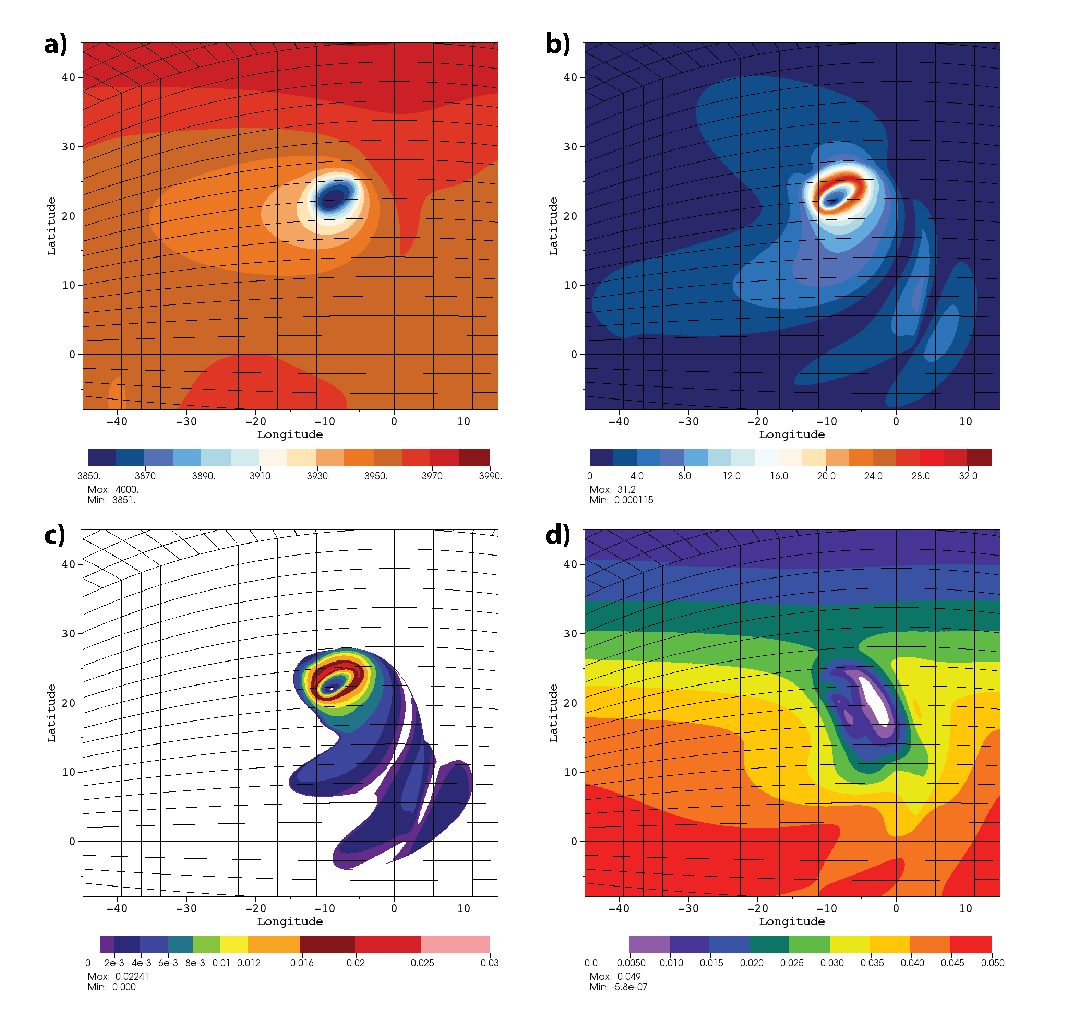
\includegraphics[width=\textwidth]{Chap2/c2048_day8_plots-01.eps}}
   \caption{Day 8 plots for the uniform c2048 run of the isolated strengthening vortex for several variables: 
   (a) Height field (m), (b) Wind magnitude (m s$^{-1}$), (c) Instantaneous precipitation rate (moisture value per day), 
   and (d) Reservoir moisture content (moisture value).
   These plot correspond to the day 8 vorticity plot in Fig. \ref{fig:c2048_vortseries}(f), though
    note the larger latitude-longitude domain in these plots. }%
    \label{fig:c2048_day8}
\end{figure}
    
   Figure \ref{fig:c2048_day8} provides a snapshot of the height field, wind magnitude, precipitation rate, and moisture reservoir at day 8, 
   corresponding to the relative vorticity profile in Fig. \ref{fig:c2048_vortseries}f.
   After eight days, the minimum height shown in Fig. \ref{fig:c2048_day8}a
   at the center of the vortex has decreased by $140$ m. The velocity magnitude
   profile depicted in Fig. \ref{fig:c2048_day8}b and the instantaneous precipitation rate 
   in Fig. \ref{fig:c2048_day8}c contain, as in the vorticity profile at day 8, an
   elongated ring of strongest winds and heaviest precipitation. to the southeast of the
   vortex center, a Rossby wave train forms as visible in the wind and precipitation
   fields (Figs. \ref{fig:c2048_day8}b,c). The ocean-like reservoir of available moisture 
   for evaporation is plotted in Fig. \ref{fig:c2048_day8}d. The area of low reservoir levels
   to the southeast of the vortex shows where evaporation has been the strongest and
   reflects the path of the vortex. 
      
\begin{figure}
    \centerline{%
    \noindent
    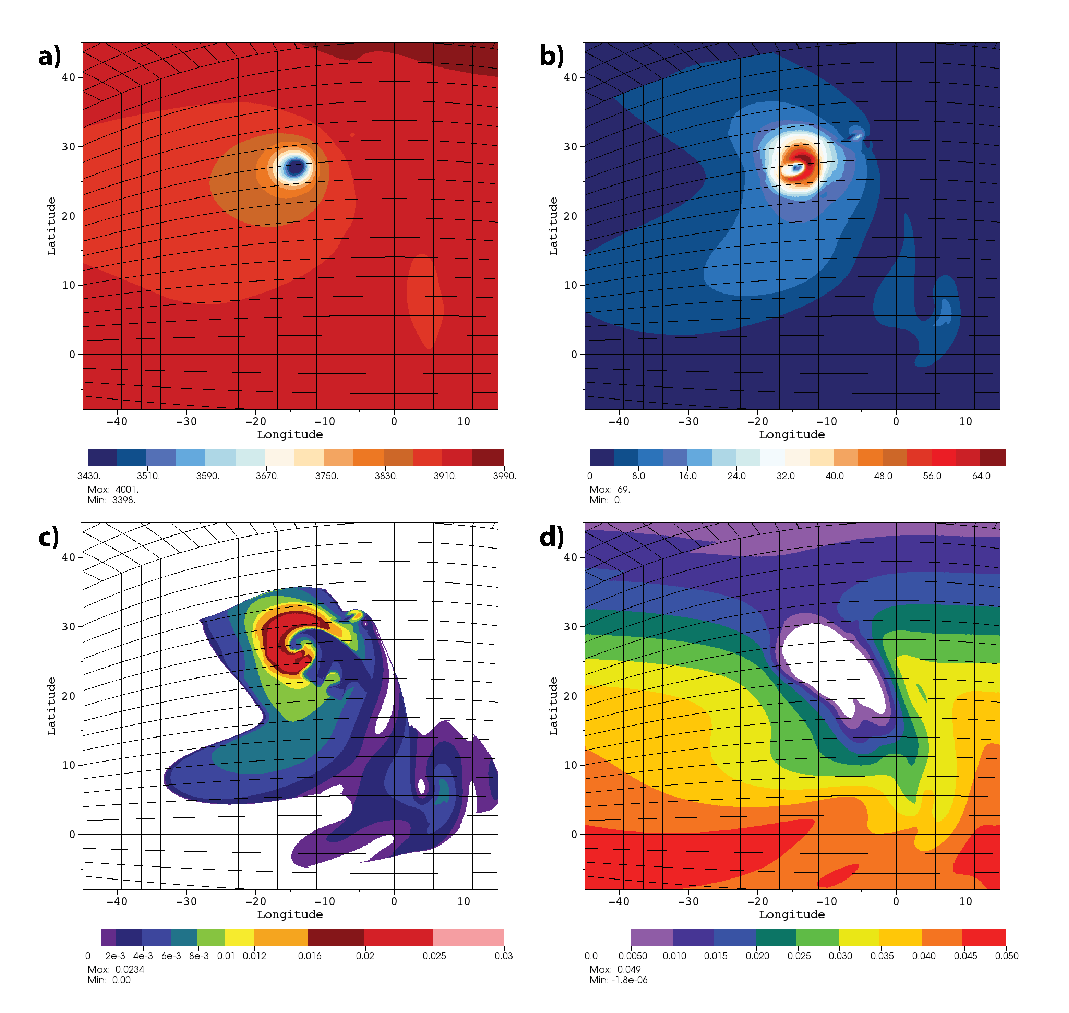
\includegraphics[width=\textwidth]{Chap2/c2048_day10_plots-01.eps}}
   \caption{Day 10 plots for the uniform c2048 run of the isolated strengthening vortex for several variables: 
   (a) Height field (m), (b) Wind magnitude (m s$^{-1}$), (c) Instantaneous precipitation rate (moisture value per day), 
   and (d) Reservoir moisture content (moisture value).
   These plot correspond to the day 10 vorticity plot in Fig. \ref{fig:c2048_vortseries}(h), though
    note the different latitude-longitude domain in these plots. }%
    \label{fig:c2048_day10}
\end{figure}

   The same fields are depicted
   for day 10 in Fig. \ref{fig:c2048_day10}. The height has decreased to a minimum of $3400$ m.
   As in the vorticity profile in Fig. \ref{fig:c2048_vortseries}h, the wind magnitude profile in 
   Fig. \ref{fig:c2048_day10}b has begun to re-form a cyclone-like profile with a central calm eye
   surrounded by a ring of maximum winds. However, the precipitation rate 
   (Fig. \ref{fig:c2048_day10}c) does not reform a symmetric ring, and precipitation is limited
   in the southeastern sector of the vortex due to a lack of additional moisture
   being evaporated. As seen in Fig. \ref{fig:c2048_day10}d, the available moisture
   for evaporation in that area has been depleted. This lack of moisture for evaporation suppresses 
   convection and vortex strengthening. A comparable real world effect is
   the cold wake reduction in ocean surface heat content that forms 
   behind the path of tropical cyclones due to the cyclone wind induced surface layer mixing.  
   The main vortex strengthen more slowly
   after day 10, as the vortex has reached higher latitudes that have less 
   moisture available in the reservoir. The maximum relative vorticity peaks after eleven days before slowly
   declining in magnitude, though the small secondary vortex continues to strengthen. 
   The main vortex wind speed follows the same trend, reaching a maximum between twelve and thirteens days with an unrealistic
   speed of $176$ m s$^{-1}$ before slowly declining.
   
           
\section{Numerical results for uniform and AMR grids}
\label{sec:wetvortresults}
Next we examine the effects of grid resolution on the evolution of the vortex and assess 
the ability of different AMR refinement criteria to achieve comparable results to uniform
resolution runs. With the high resolution c2048 run serving as a reference,
we implement the test case with the resolutions listed in Table \ref{tb:grids2}.
In addition, we conduct a variety of runs with AMR based on 
4 different tagging criteria sets to determine the optimal tagging criterion. 
The differences between these sets are (a) the magnitude of the absolute value of the relative 
vorticity threshold, on which the criteria are refined, and (b) the change in that threshold between multiple
levels of AMR. We implement two types of thresholds.
The first is a constant threshold in which the required vorticity value is the same 
across all resolutions and, when met, all the AMR levels are added simultaneously.
The second version is a scaled threshold that increases with the level's resolution.
In this setup, one level of refinement is implemented when the threshold value is met, but
the next level of AMR is not added until a new, higher threshold value scaled with the increasing resolution is reached.
For example, a three level AMR run with x4 refinement, a base resolution of $c32$, 
and a vorticity tag threshold of 
$|\zeta| > 2$ days$^{-1} = 2.3 \times 10^{-5}$ s$^{-1}$ will implement
the first AMR level at a c128 resolution once that threshold has been exceeded. With this new
resolution of c128, the threshold is four times higher 
$|\zeta| > 8$ days$^{-1} = 9.3 \times 10^{-5}$ s$^{-1}$ 
in regions covered by the first level of AMR. This causes the second
level of refinement, with a c512 resolution, to not implement until the vorticity has 
exceeded this new higher threshold. This delay in triggering higher refinement results 
in some loss of detail on features of interest in their initial stages, but fewer grid cells, 
and thus computational cost, are added until absolutely necessary.
For AMR with only one level of refinement, there is no difference between
the two threshold scalings.
The four tagging criteria are:
\begin{itemize}
    \item
        Tag 1: a vorticity threshold that scales with resolution 
        with a base level threshold of 
        $|\zeta| > 2$ days$^{-1} = 2.3 \times 10^{-5}$ s$^{-1}$
     \item
        Tag 2: a vorticity threshold that scales with resolution 
        with a base level threshold of 
        $|\zeta| > 3$ days$^{-1} = 3.5 \times 10^{-5}$ s$^{-1}$
     \item
        Tag 3: a vorticity threshold that scales with resolution 
        with a base level threshold of 
        $|\zeta| > 8$ days $^{-1} = 9.3 \times 10^{-5}$ s$^{-1}$
     \item
        Tag 4: a constant threshold across all AMR levels for vorticity of 
        $|\zeta| > 5$ days $^{-1} = 5.8 \times 10^{-5}$ s$^{-1}$.
\end{itemize}
The higher vorticity threshold in Tag 4 compared to the scaled thresholds in 
Tags 1 and 2 attempts to reduce the computational cost of the constant threshold
method and make the model more comparable to that of the scaled threshold methods. Tag 3 simply increases 
the threshold by four times that of Tag 1 so that a c32 base level AMR with x4 refinement
using Tag 1 will have the same threshold of refinement for its second level of AMR as a c128 base level
AMR using Tag 3 has for its first level of AMR.

We focus on the vorticity field in this analysis, as it contains a combination of large-scale 
and fine-scale structures and is sensitive to changes in resolution. The height and
velocity fields have fewer small-scale features and the minimum height and maximum wind
associated with the main vortex correlate well to the vorticity strength. The precipitation
field is also larger in scale and has little variability with resolution.

Focusing on the single isolated vortex, Fig. \ref{fig:vort_lineplot} depicts the growth of the vortex with a daily
maximum magnitude of relative vorticity for uniform resolution runs (Fig.
\ref{fig:vort_lineplot}a), AMR runs using tags 1 and 3 (Fig. \ref{fig:vort_lineplot}b), AMR runs 
with tag 2 (Fig. \ref{fig:vort_lineplot}c), and AMR runs with tag 4 (Fig. \ref{fig:vort_lineplot}d).
The line color for each AMR run corresponds to base level resolution while the line style corresponds
to the resolution of the highest AMR level. The uniform runs in Fig. \ref{fig:vort_lineplot} serve as the
reference for the color and style of each resolution. 

\begin{figure}
   \centerline{%
   \noindent
   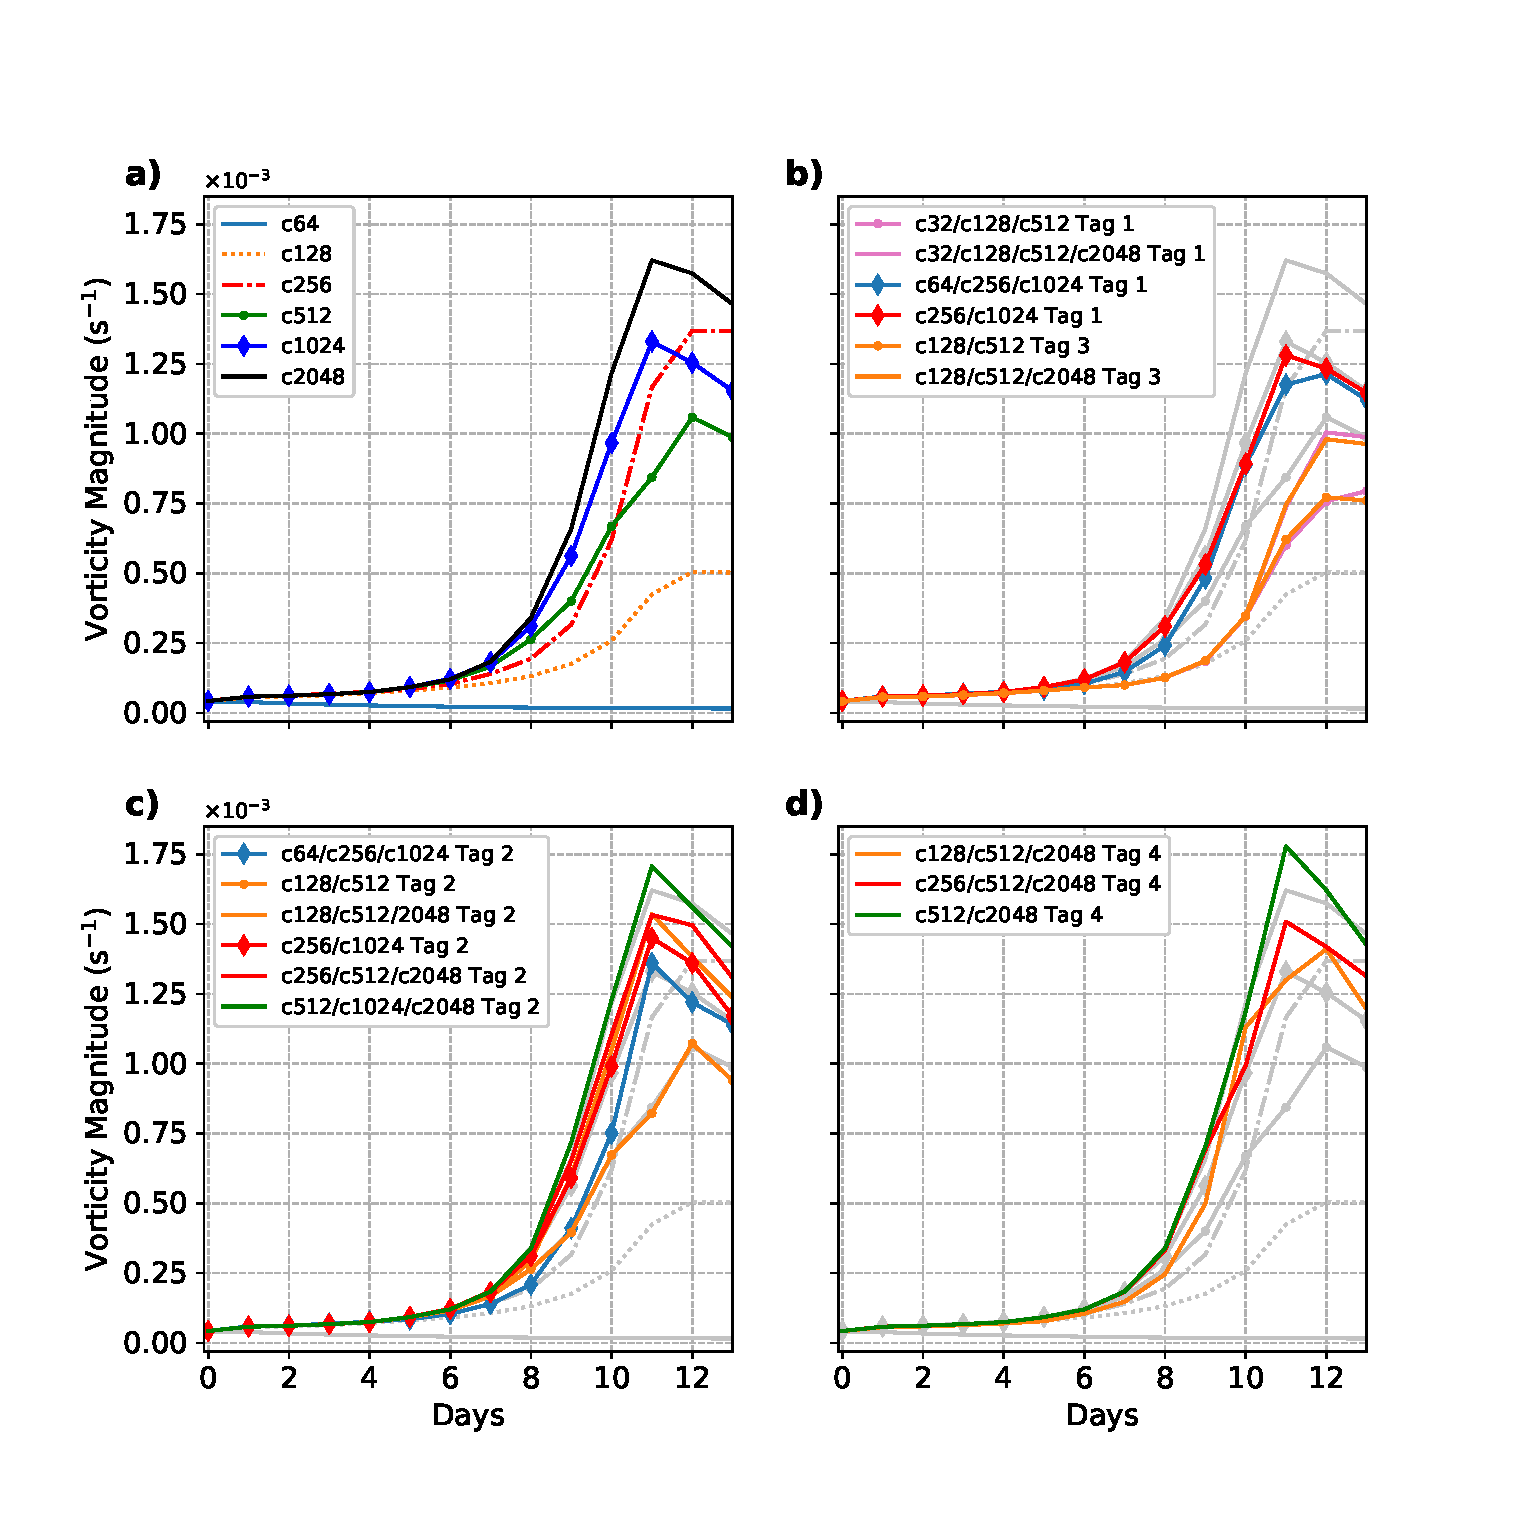
\includegraphics[width=\textwidth]{Chap2/vortmax_lineplot.eps}}
   \caption{Maximum relative vorticity of the strengthening vortex over a 
   period of 13 days for (a) uniform runs, (b) AMR runs using the Tag 1 or
   Tag 3 refinement criteria, (c) AMR runs using the Tag 2 criteria, and (d)
   AMR runs using the Tag 4 criteria. All the plots follow a line color and marker
   system dependent on resolution. The line color denotes the run's base resolution
   while the line style denotes the run's highest AMR resolution. The line color and
   style for each resolution is as follows: c2048 (black, plane), c1024 (blue, solid diamond markers),
   c512 (green, small circle markers), c256 (red, dot-dash line), and c128 (orange, dotted line).
   The coarse resolutions c64 and c32 have only a line color, light blue and pink respectively, and
   no line style as none of the AMR runs have a highest refinement at these resolutions given that
   the vortex does not develop on such a coarse grid (as seen by the c64 uniform run in (a)).
   For comparison purposes the uniform run lines from (a) have been imposed in light grey on
   the other three plots.
   }
   \label{fig:vort_lineplot}
\end{figure}

Overall vortices with higher resolution have larger
maximum vorticity over the first nine days. The c64 resolution has not strengthened, nor has
the c32 resolution, which is not plotted in Fig. \ref{fig:vort_lineplot}a. 
In these cases, the grid resolution is
too coarse and the initialized vortices slowly weaken.
In Fig. \ref{fig:vort_lineplot} we see the c256 run strengthening 
more rapidly after day 9 than higher resolution runs such
that its maximum vorticity is higher than the c512 and c1024 runs by day 12.  Over the same time 
period we see that the c512 and higher resolution runs reach a peak strength between day 11 and day 12
before slowly decreasing, observing a regime change that the coarser resolution c256 and c128 are not
able to resolve. This regime change can be seen in Fig. \ref{fig:uni_d9nd12}, which 
depicts the relative vorticity field for uniform runs c256, c512, and c1024 at day 9 in
Figs. \ref{fig:uni_d9nd12} (a)-(c) and day 12 in Figs. \ref{fig:uni_d9nd12}(d)-(f).

\begin{figure}
   \centerline{%
   \noindent
   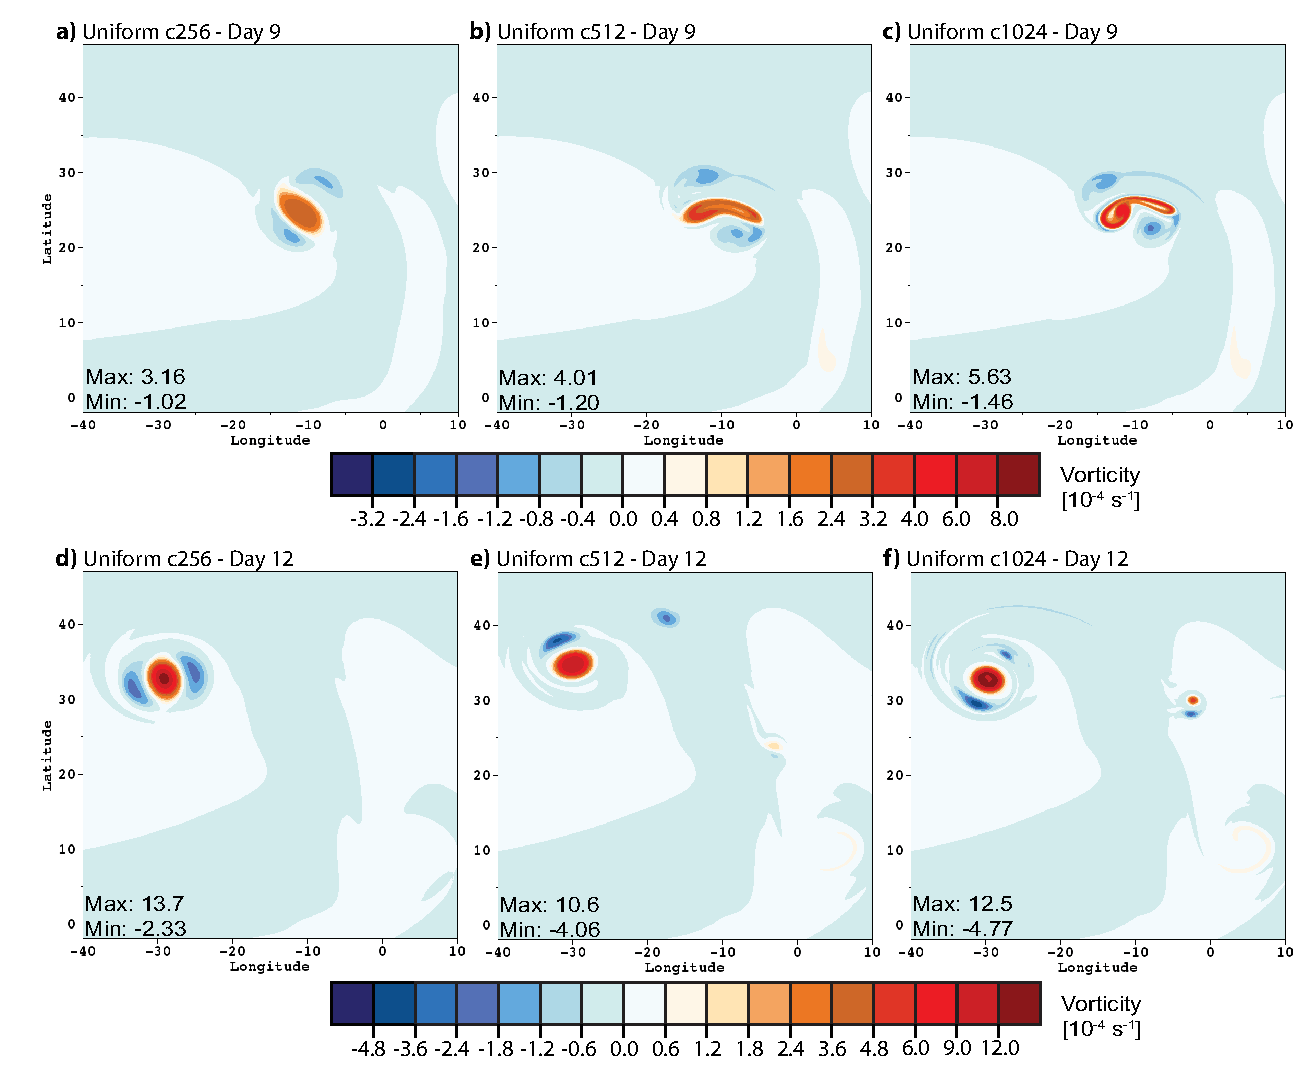
\includegraphics[width=\textwidth]{Chap2/uni_runs_day9n12-01}}
   \caption{Relative vorticity field of the 
   strengthening vortex case at day 9 (a) - (c) and day 12 (d)-(f) for uniform runs 
   c256 resolution (a) and (d), c512 resolution (b) and (e), and 
   c1024 resolution (c) and (f). These plots
   correspond to the day 9 uniform c2048 plot, Fig. \ref{fig:c2048_vortseries}g, and
   day 12 plot Fig. \ref{fig:c2048_vortseries}i.
   }
   \label{fig:uni_d9nd12}
\end{figure}

Comparing day 9 in Fig. \ref{fig:uni_d9nd12} and Fig. \ref{fig:c2048_vortseries}g,
the strength of the vortex is clearly dependent on resolution, as the maximum vorticity
increases with each resolution. The structure of the vortex, however, visually 
converges. The ring collapse and roll-up seen at day 9 in the 
uniform c2048 run in Fig. \ref{fig:c2048_vortseries}g
is also observed in the c1024 run (Fig. \ref{fig:uni_d9nd12}c) 
despite the slightly weaker maximum vorticity.
The weaker vortex of the uniform c512 run results in a delay of the 
stretching and collapse of the vortex ring. In Fig. \ref{fig:uni_d9nd12}b,
the vortex is stretched, but the roll-up has not begun. The ring
structure is still visible but less distinct as in the higher resolution runs.
In the uniform c256 run the vortex does not form a distinct vortex ring structure 
and continues to strengthen at day 9 without a significant
change to its structure. (Fig. \ref{fig:uni_d9nd12}a).

By day 12, the c1024 vorticity filaments have rolled back up into a single vortex and spun off
a smaller secondary vortex with a vorticity dipole feature. The field is visually
similar to the c2048 run at day 12 in Fig. \ref{fig:c2048_vortseries}i, 
albeit slightly weaker overall and thus less northward by day 12. 
Since the c256 run did not undergo the collapse and roll-up,
its maximum vorticity at day 12 in Fig. \ref{fig:uni_d9nd12}d is now stronger 
than that of the c512 and c1024 vortices.  In addition, no secondary vortex develops.
The uniform c128 run follows a similar, though weaker evolution, so it is not shown here. 
For the c512 uniform run at day 12 in Fig. \ref{fig:uni_d9nd12}e, a secondary vortex has spun off 
(centered around $(25^\circ N, -3^\circ W)$ but is significantly weaker than the secondary vortices 
in the c1024 and c2048 runs. In addition, one of the two anticyclonic regions that abut the main 
vortex in the c1024 and c2048 runs has been spun off as well. Figure \ref{fig:uni_d9nd12}
shows these two different regimes are dependent on resolution. At resolutions c256 and below
the development of a distinct vortex ring and its collapse cannot be resolved. The c512
resolution appears to be the start of the high resolution regime, 
which begins to converge between the c1024 and c2048 resolution runs.

The AMR runs shown in Figs. \ref{fig:vort_lineplot}(b)-(d) do an 
effective job of following the growth trajectory of uniform run with the same resolution as 
the finest AMR level with a few exceptions. 
However, several AMR maximum vorticity values remain lower than the corresponding uniform run.
This occurs because the higher resolution refinement is not implemented early enough in the simulation,
resulting in the lower strength observed in the uniform c256 and lower resolutions runs.
This can be seen in the c128/c512/c2048 AMR with Tag 4 in Fig. \ref{fig:vort_lineplot}d.
The refinement levels in that run are triggered at day 2, and the resulting delay
causes the maximum strength to remain below the uniform c2048 level throughout
the thirteen days of the simulation. The largest divergence occurs for the c32 AMR runs
with Tag 1 and c128 AMR runs with Tag 3 in Fig. \ref{fig:vort_lineplot}b. 
The two runs with the highest AMR level of c2048 have a maximum vorticity
nearly 40\% weaker at day 12 than the uniform c2048 run. The other two AMR runs, with a highest
AMR level of c512, are approximately 25\% weaker than the c512 uniform vortex. These runs also 
follow the low resolution regime more closely than the regime expected by their highest AMR level. 
All four of these runs begin with a highest resolution of c128, as the Tag 1 threshold for c32 AMR runs 
triggers the c128 level of refinement immediately at initialization.  However, for both the c32 AMR Tag 1 runs
and the c128 Tag 3 runs, the c512 AMR level is not triggered until six and a half days into the simulation,
and the two runs which reach the c2048 level resolution do not trigger it until day 10. As a result, the model benefits
of instituting this higher resolution occur too late in the simulation. As Fig. \ref{fig:vort_lineplot}b shows, these four
runs do not diverge from the c128 uniform run until
day 9. In other AMR setups, the delayed implementation of
the highest AMR resolution does not degrade the growth 
of the vortex strength. For the c64/c256/c1024 AMR 
runs with Tag 1 and Tag 2 refinement, the first refinement 
level of c256 resolution is triggered initially.
The second c1024 level, however, is not triggered until 
after five days or seven days, for Tag 1 and Tag 2, respectively.  
As a result, we observe that the c64 AMR run with Tag 1 in 
Fig. \ref{fig:vort_lineplot}b does not diverge from the uniform c256
run until after day 7, and in Fig. \ref{fig:vort_lineplot}c 
the c64 Tag 2 AMR run does not diverge until after day 8.
Both, however, follow the c1024 maximum vorticity closely by day 10.
Though delayed, the refinement still occurs before the rapid intensification period during which
the developing vortex becomes unstable and collapses. 
Thus these two runs are able to more successfully
match the c1024 uniform results than the c32 Tag 1 AMR 
runs. In the cases of the c512/c2048 AMR runs, the AMR results in a 
slightly higher maximum vorticity than the corresponding 
uniform run between day 10 and day 12 using 
Tag 2 (Fig. \ref{fig:vort_lineplot}c) and Tag 4 (Fig. \ref{fig:vort_lineplot}d)  
as well as with the c256/c1024 AMR run using Tag 2 (Fig. \ref{fig:vort_lineplot}c).

\begin{figure}
   \centerline{%
   \noindent
   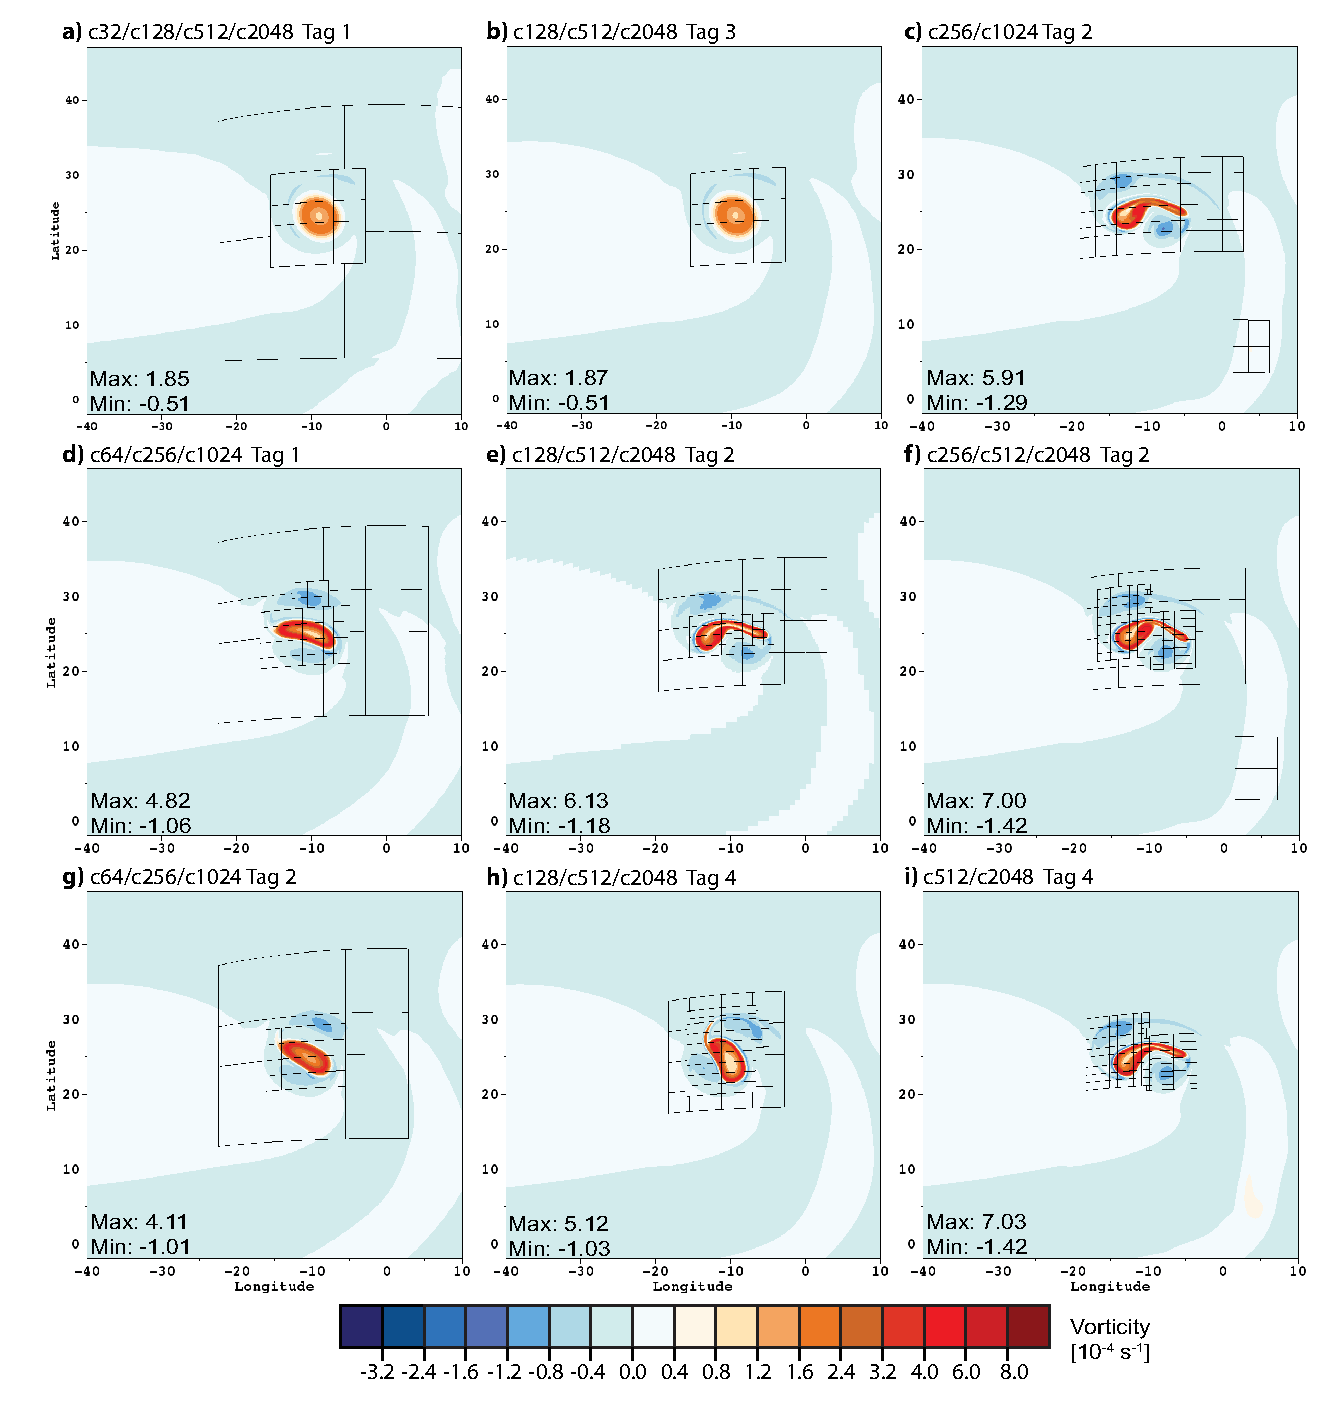
\includegraphics[width=\textwidth]{Chap2/day9_vort-01.eps}}
   \caption{Relative vorticity fields at day 9 for several AMR runs of the 
   strengthening vortex case. (a) c32 base 4-level AMR run with x4 
   refinement using Tag 1. (b) c128 base 2-level AMR run with
   x4 refinement using Tag 3.
   (c) c256 base 1-level AMR run with x4 refinement using Tag 2.
   (d) c64 base 2-level AMR run with x4 refinement using Tag 1.
   (e) c128 base 2-level AMR run with x4 refinement using Tag 2.
   (f) c256 base 2-level AMR run with one level of x2 refinement 
   and one of x4 refinement using Tag 2.
   (g) c64 base 2-level AMR run with x4 refinement using Tag 2.
   (h) c128 base 2-level AMR run with x4 refinement using Tag 4.
   (i) a c512 base 1-level AMR run with x4 refinement using Tag 4. These plots
   correspond to the day 9 uniform plots in Fig. \ref{fig:c2048_vortseries}g and
   \ref{fig:uni_d9nd12}(a)-(c). The block structures of the multiple refinement
   levels are outlined in black
   }
   \label{fig:vort_amr_day9}
\end{figure}

Figures \ref{fig:vort_amr_day9} and \ref{fig:vort_amr_day12} depict the relative 
vorticity field for day 9 and day 12 respectively for nine AMR runs. They provide 
a more detailed comparison of the overall vortex and the small-scale features in the 
vorticity field between the AMR runs and the uniform resolution runs in 
Fig. \ref{fig:c2048_vortseries} and Fig. \ref{fig:uni_d9nd12}. At day 9, the selected
AMR runs in Fig. \ref{fig:vort_amr_day9} are at various stages of the 
evolution process, depending on their resolutions and tagging criteria. As in 
Fig. \ref{fig:vort_lineplot}b, the c32 base 4-level AMR with Tag 1 run (Fig. 
\ref{fig:vort_amr_day9}a) and the c128 2-level AMR with Tag 3 run (Fig.
\ref{fig:vort_amr_day9}b) are significantly weaker than the uniform c2048 run
at day 9 (Fig. \ref{fig:c2048_vortseries}g). The highest level of AMR for both runs, c2048,
has not yet been triggered, and both runs use c512 resolution over the vortex.
 The evolution of the vortex corresponds to the high resolution regime, albeit delayed, with the clearly visible
 vortex ring. Figures \ref{fig:vort_amr_day9}a and b are more comparable to
the c2048 uniform run at day 6 (Fig. \ref{fig:c2048_vortseries}d). Though not as pronounced,
the two c64 based AMR runs are also delayed in their vortex evolution. The c64 2-level AMR runs
with Tag 1 (\ref{fig:vort_amr_day9}d) and Tag 2  (\ref{fig:vort_amr_day9}d) both have a clearly
defined vortex ring that has begun to stretch and deform. However, they are more similar 
in strength and appearance to the c512 uniform run at day 9 in Fig. \ref{fig:uni_d9nd12}b. 
In addition, the vortex in the c64 Tag 1 run is slightly stronger and more deformed, reflecting the
two day advantage provided by the Tag 1 criteria in which the c1024 AMR level is triggered at a lower threshold.

The c128 and higher resolution base level AMR runs are able to capture the vortex roll-up
effectively at day 9. The three AMR runs using Tag 2 refinement criteria, 
c256/c1024 (Fig. \ref{fig:vort_amr_day9}c), c128 2-level AMR
(Fig. \ref{fig:vort_amr_day9}e), and c256 2-level AMR (Fig. \ref{fig:vort_amr_day9}f,
as well as the c512 1-level AMR Tag 4 refinement criteria run (Fig. \ref{fig:vort_amr_day9}i)
capture the collapse and roll-up of the vortex and closely match the day 9 vorticity magnitudes
seen in the c1024 and c2048 uniform runs.
The AMR runs are also able to resolve  the two areas of negative vorticity 
on either side of the main vortex. However, the roll-up process in the AMR runs is slightly
delayed compared to the high resolution uniform runs. The distinct comma-like positive vorticity 
feature of the main vortex ring seen in the uniform c2048 (Fig. \ref{fig:c2048_vortseries}g) and c1024 (Fig. \ref{fig:uni_d9nd12}c) runs
is not as prominently developed in these AMR runs. 
An exception to this is observed in the c128 base 2-level AMR run with Tag 4. Seen in
Fig. \ref{fig:vort_amr_day9}h, the vortex ring in this Tag 4 run (Fig. \ref{fig:vort_lineplot}d )
is approximately 25\% weaker than the c2048 uniform run and the vortex
roll-up is slowed by half a day. Both the slight ring deformation and the northward extension of the positive vorticity filament 
from the northwest sector of the vortex ring correspond well to the structure of
the vortices in the uniform c1024 and c2048 runs at 8.5 days. 

\begin{figure}
   \centerline{%
   \noindent
   \includegraphics[width=\textwidth]{Chap2/day12_vort-01.eps}}
   \caption{Same as Fig. \ref{fig:vort_amr_day9}, but for day 12 after the small
   secondary vortex has spun off. These plots correspond to the day 12 uniform
   plots in Fig. \ref{fig:c2048_vortseries}i and \ref{fig:uni_d9nd12}(d)-(f). 
   The block structures of the multiple refinement
   levels are outlined in black
   }
   \label{fig:vort_amr_day12}
\end{figure}

Figure \ref{fig:vort_amr_day12} depicts the vorticity fields of the AMR runs after vortex ring collapse
and spin-off of a smaller secondary vortex. The c256 and c512 base resolution AMR runs (Figs.
\ref{fig:vort_amr_day12}c, f, and i) exhibit vorticity 
maximums roughly 10\% higher than their corresponding high resolution 
uniform runs reflecting Fig. \ref{fig:vort_lineplot}. These three AMR runs most closely resemble
the formation and location of the secondary vortex and capture the anticyclonic
 filaments wrapping aground the main vortex.
The six AMR runs with coarser base resolutions have lower peak magnitudes. The 
vorticity fields for the c32 Tag 1 AMR run in Fig. \ref{fig:vort_amr_day12}a and the
c128 Tag 3 AMR run in Fig. \ref{fig:vort_amr_day12} show delayed spin-offs of 
the secondary vortex and less symmetric main vortices,
comparable to day 10 of the c2048 uniform run in Fig. \ref{fig:c2048_vortseries}h.
The c64 2-level AMR Tag 1 run in Fig. \ref{fig:vort_amr_day12}d has a vorticity 
maximum similar to the c1024 uniform reference. This AMR run also resolves 
the secondary vortex, though its position is further to the northwest than that of the c1024 uniform run shown
in Fig. \ref{fig:uni_d9nd12} at day 12. In contrast,
the slightly higher threshold of Tag 2 refinement criteria 
combined with the c64 2-level AMR run (Fig. \ref{fig:vort_amr_day12}g) 
is unable to reproduce the secondary vortex spin-off. The
c128 AMR runs depicted in Fig. \ref{fig:vort_amr_day12}e and h both demonstrate development of
a secondary vortex, though the Tag 2 run is more chaotic.
This is shown by the large negative voricity filament area around the Tag 2 run secondary vortex and a weak third cyclonic vortex.
The anticyclonic filaments are also more defined for the c128 2-level AMR Tag 4 run (Fig. \ref{fig:vort_amr_day12}h)
than the Tag 2 run in Fig. \ref{fig:vort_amr_day12}e. 

\begin{figure}
   \centerline{%
   \noindent
   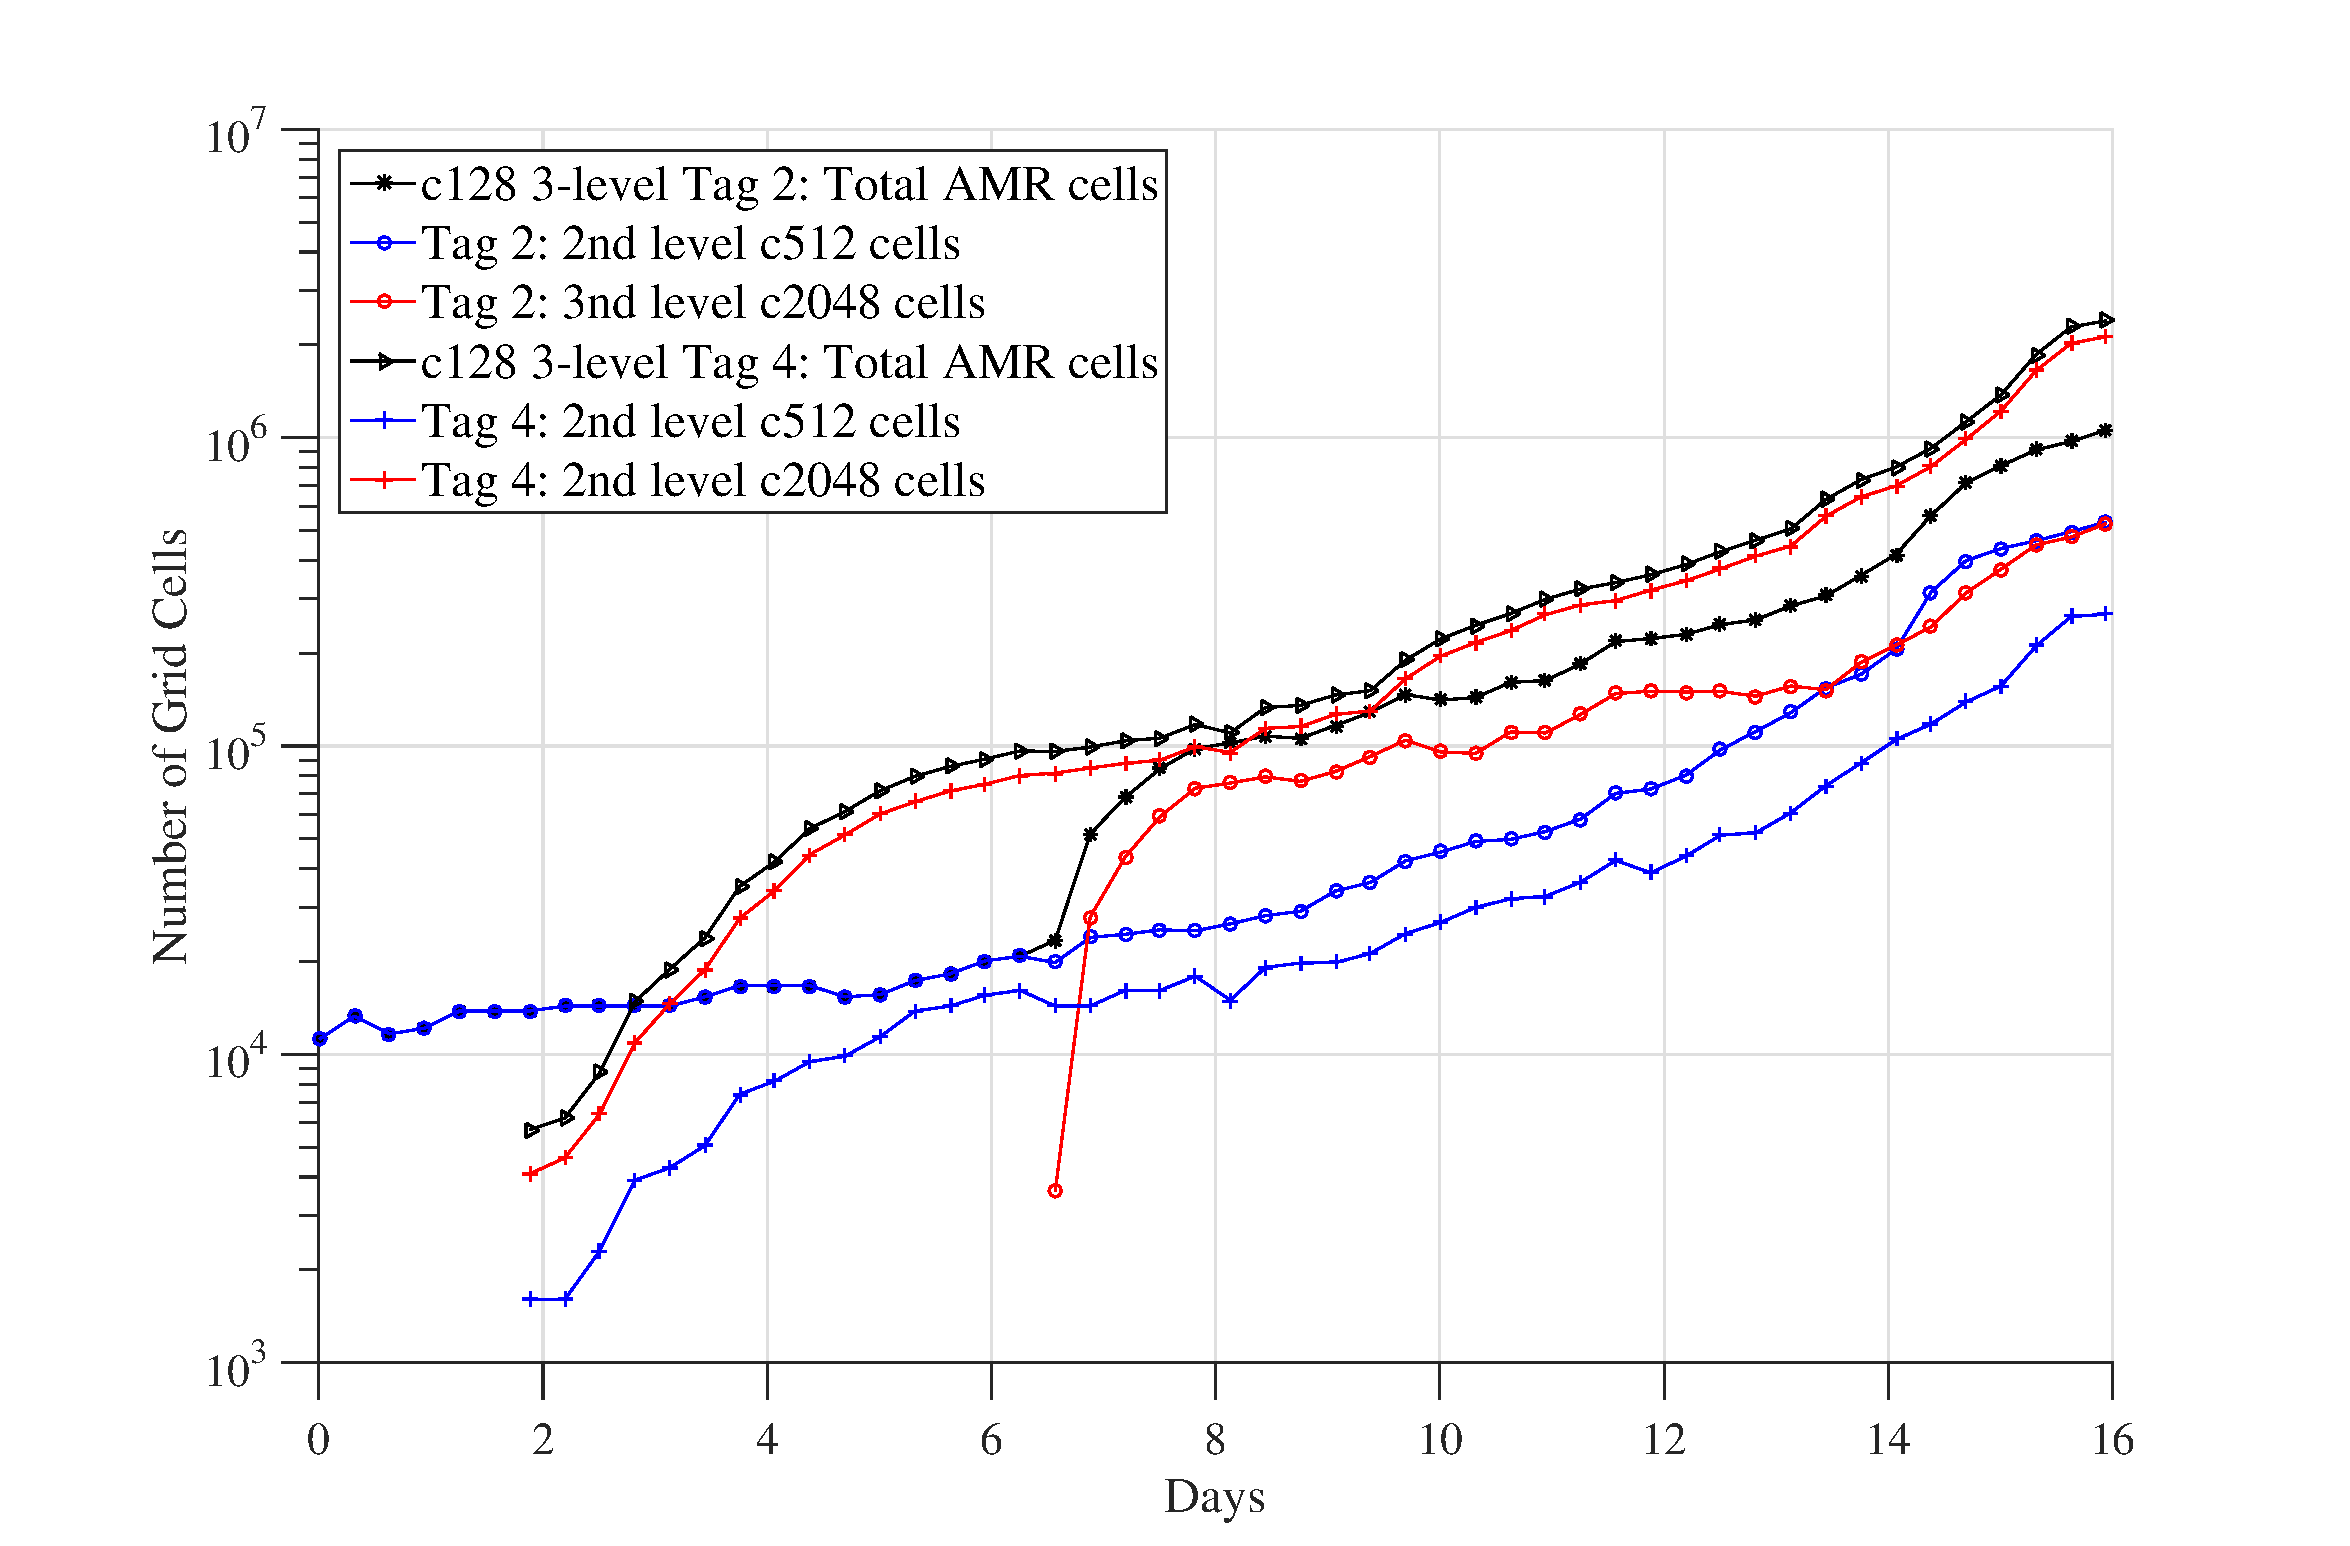
\includegraphics[width=\textwidth]{Chap2/c128_3l4_Tag2vs4_compare.eps}}
   \caption{The growth of AMR grid cells over time for the two c128 2-level AMR runs 
   with tag 2 and tag 4 refinement criteria. The base level c128 grid cells are excluded
   while the 2nd level c512 cells are plotted in blue and the third level c2048 cells are
   plotted in red with a plus marker to denote the tag 4 run and a circle to denote the
   tag 2 run.  The sum of the two levels are plotted in black with a triangle marker denoting
   the tag 4 run and an asterisk marking the tag 2 run. 
   }
   \label{fig.grid_num_c128}
\end{figure}

Figure \ref{fig.grid_num_c128} shows the number of grid cells at each AMR 
level as a function of time for both c128 2-level AMR runs.  While the lower 
base level refinement threshold in Tag 2 results in the c512 level AMR being applied
initially, refinement does not occur for two days with the Tag 4 criteria, at which time
both levels of refinement are implemented due 
to the constant threshold value. Though both levels are implemented,
the c2048 refinement level 
covers only the center core of the vortex and 
the outer edges of the vortex remain at
c512 or c128 resolution for another day.
After day 3, the Tag 4 run has almost 10x more 
cells than the Tag 2 run. That difference narrows significantly once the c2048
level is triggered for the Tag 2 run after day 6. 
Through the entire 16 day simulation, the Tag 2 run has more c512 grid
cells while the Tag 4 run has more c2048 cells. Therefore, though the Tag 4 run
has more grid cells and has triggered the c2048 refinement level for four days more than the 
c128 2-level AMR Tag 2 run, the Tag 2 run better captures the vortex roll-up at day 9 
(Figs. \ref{fig:vort_amr_day9}e and h).
The c512 resolution gained earlier, in the first two days, appears to outweigh the benefits 
of more c2048 resolution throughout the majority of the run time. 
The benefit of that early advantage fades as the run continues, and the benefit of more coverage by
the c2048 refinement level becomes apparent. By day 12 
the c128 Tag 2 run lacks the c2048 resolution around the core of the main 
vortex needed to resolve the thin negative vorticity filaments (Fig. \ref{fig:vort_amr_day12}e), 
which the Tag 4 run is able to capture (Fig. \ref{fig:vort_amr_day12}h). 
The secondary vortex in the Tag 4 run also more closely resembles the uniform c2048 run.

A key delineation between these AMR runs is apparent 
when c512 resolution or higher is implemented. At these 
levels of refinement, the vortex undergoes the high resolution evolution regime.
The AMR runs with tagging criteria that triggered refinement levels 
of at least c512 initially, or within the first day, exhibited 
vortex growth most similar to the uniform c2048. 
The subset of these runs that do not trigger the c2048 
refinement level until well into the simulation (six days or later)  
outperform AMR runs which have coarser than c512 resolutions 
initially but trigger c2048 resolution much earlier. 
Refinement, no matter what time it is applied still improves the results. 
Once c512 or higher refinement is triggered, rapid strengthening occurs 
and the vortex eventually transition to the high resolution evolution 
regime. The critical vortex collapse merely occurs later in time and we
see some of those AMR runs can catch-up to the 
reference solution run by day 10 or 12.

     \subsection{Extended Run Results} \label{sec:extended}
Extending the simulation time leads to development of an active and complex global flow pattern.
The isolated vortex discussed in detail in the previous sections, as well as the binary
pair of weaker vortices, evolve independently of each other for twelve days. 
Beyond twelve days, the Rossby wave trains, though small in magnitude,
spread and trigger evaporation and convection over a significant area.
As a result, by day 16 of the simulation, a global chaotic flow has developed with multiple unseeded
cyclonic and anticyclonic areas.  Additionally, jet-like features
develop around the $30^\circ$N and S latitudes which correspond to the areas of transition between high and low moisture 
as determined by the initial moisture field and reservoir.
Figure \ref{fig:threevort_uni} depicts vorticity fields of all three vortices 
at day 9 and day 12 as well as the resulting global vorticity field at day 16
for uniform c256 (Fig. \ref{fig:threevort_uni}a), c512 (Fig. \ref{fig:threevort_uni}b),
c1024 (Fig. \ref{fig:threevort_uni}c), and c2048 (Fig. \ref{fig:threevort_uni}d) resolution
runs. The plots for day 9 and 12 are restricted to the three vortices as
these are the primary features during that time frame. Day 16 plots depict the 
global relative vorticity field. The overall flow, number of large-scale vortices,
and vortex locations remain fairly consistent across the increasing uniform resolutions.
The higher resolutions naturally resolve more fine-scale structures in this chaotic system, though
the uniform c1024 and c2048 runs also resolve several small-scale vortices as can be observed around $15^\circ$N and $30^\circ$W and nearby anticyclonic patches The high maximum vorticity in the c2048 run at day 16 is from the cyclonic vortex centered near $15^\circ$N and $30^\circ$W.

\begin{figure}
   \centerline{%
   \noindent
   \includegraphics[width=\textwidth]{Chap2/global_uni_vort-01.eps}}
   \caption{Late run evolution of the relative vorticity field for the 
   strengthening vortex case with three initialized vortices. These plots show
   the growth of a global chaotic regime by day 16 in for uniform resolution
   runs. Relative vorticity snapshots at days 9 (left column), 12 (middle column), 
   and 16 (right column) are given for
   (a) uniform c256 run, (b) uniform c512 run, (c) uniform c1024 run, and
   (d) uniform c2048 run. The leftmost vortex in the days 9 and 12 plots
   located around $(30^\circ \mathrm{N}, 15^\circ \mathrm{W})$ is the isolated
   vortex discussed in previous sections. The two vortices centered around
   $(20^\circ \mathrm{N}, 90^\circ \mathrm{E})$ are the binary pair. Note: the
   vorticity extrema occur in the isolated vortex in all cases for days 9 and 12 so they are 
   not displayed.}
   \label{fig:threevort_uni}
\end{figure}
\begin{figure}
   \centerline{%
   \noindent
   \includegraphics[width=\textwidth]{Chap2/day16_vort-01.eps}}
   \caption{Relative vorticity fields at day 16 for four AMR runs of the strengthening
   vortex case with three initialized vortices: 
   (a) c64 base 2-level AMR run with x4 refinement using Tag 2,
   (b) c128 base 2-level AMR run with x4 refinement using Tag 2,
   (c) c256 base 1-level AMR run with x4 refinement using Tag 2,
   and (d) c256 base 2-level AMR run with one level of x2 refinement 
   and one of x4 refinement using Tag 2. The left column depicts the vorticity 
   field at day 16 while the right column overlays
   the block structures of the refinement levels in black. These plots
   are comparable to the day 16 plots in Fig. \ref{fig:threevort_uni}.
   }
   \label{fig:vort_amr_day16}
\end{figure}

In addition to the uniform runs, we extend four AMR runs to 16 days of simulation. 
The global vorticity fields at day 16 for these runs are plotted in 
Fig. \ref{fig:vort_amr_day16}. The first column depicts the relative vorticity,
while the second shows the block structure for the multiple AMR levels.
All four AMR runs capture the overall jet-like flow of the system.
The c64 base 2-level AMR run in Fig. \ref{fig:vort_amr_day16}a captures all the features
with its intermediate AMR level. However, the highest c1024 level is limited to the main vortices
and a few of the larger filaments. Thus much of the secondary flow and 
small scale features in this chaotic system diverge from 
the high resolution uniform runs. The c128 base
2-level AMR run in Fig. \ref{fig:vort_amr_day16}b, the c256/c1024 AMR run in Fig. 
\ref{fig:vort_amr_day16}c, and the 2-level c256/c512/c2048 AMR run in Fig.
\ref{fig:vort_amr_day16}d all have a high resolution level over much of the critical areas that
is better able to capture the small scale filaments and 
features. The one key metric in which the latter 
three AMR runs differ from their corresponding highest resolution
uniform run is in the maximum vorticity. In the AMR runs, as in the c1024 and c2048 
uniform runs, the vorticity maxima and minima are located in the small scale vortices
that develop. However, these extremes for the AMR runs in Figs. 
\ref{fig:vort_amr_day16}b, c, and d are more than double the values seen in the uniform runs.
The $2.53 \times 10^{-3}\mathrm{s}^{-1}$ maximum in the c128 three-level run and
the $3.81 \times 10^{-3}\mathrm{s}^{-1}$ maximum in the c256 three-level run arise
from small-scale vortices covered by small patches of the 
highest level of refinement.  The maximum in the c256/c1024 AMR run
is equally large compared to its uniform run counterpart  
($1.8 \times 10^{-3}\mathrm{s}^{-1}$) and is centered
in a broad area of refinement that had been in place for several days. These vortices
are well resolved with more than ten grid cells across and a significant buffer of refinement between the
vortices and coarse-fine boundaries. Therefore it
seems unlikely that these large vorticity values are being formed at AMR level boundaries.
The cause is more likely to be the chaotic nature of this system at day 16.

%%%%%%%%%%%%%%%%%%%%%%%%%%%%%%%%%%%%%%%%%%%%%
\section{Kessler-like Physics for Shallow Water Equations}
\label{sec:kesslersw}
An alternative setup for a moist forced shallow water system presented in 
\cite{zerroukat2015moist} derives the 2D shallow water equations from 
the moist Boussinesq equations. It includes a three-state moist physics 
model that simulates water vapor, cloud vapor, and liquid water, 
similar to the simplified 3D physics scheme presented in 
\cite{kessler1969distribution}. The forcing setup
is comparable to the generalized shallow water equations of Ripa's 
model \citep{ripa1993conservation,ripa1995improving} 
used in ocean modeling.  
In this model, latent heat released due to precipitation increases 
the average potential temperature of the fluid, which is coupled
to the momentum equations. The model can be viewed as a
diabatic non-convective model in contrast to the system used in Section \ref{sec:forcedvort} 
which can be considered an adiabatic convective 
model. It assumes energy released during
precipitation has no effect on the temperature and instead 
produces convection represented as a mass flux. A
brief discussion comparing the two models
is presented in Appendix A of \cite{bouchut2009fronts}.
We implement this physics forcing here for both uniform and
AMR runs of the barotropic instability test case of
\cite{galewsky2004initial}.

\subsection{The Shallow Water and Physics Equations}
\cite{zerroukat2015moist} dimensionally reduce the Boussinesq equations 
to obtain a derivation of the shallow water equations that retain some
buoyancy terms. These augmented shallow water equations are presented below in flux-form:
   \begin{equation}
     \label{eq:swkesmom} \frac{\partial h \mathbf{v}}{\partial t} +
     \nabla \cdot (h \mathbf{v} \mathbf{v}) + f \mathbf{\hat{k}}\times(h\mathbf{v}) + gh\nabla H = 
     g h \theta \nabla h_b + g\nabla (\frac{1}{2}h^2\theta)
   \end{equation}
   \begin{equation}
     \label{eq:swkescon}  \frac{\partial h}{\partial t} + \nabla \cdot (h\mathbf{v}) = 0
   \end{equation}
   \begin{equation}
     \label{eq:swthetacon}  \frac{\partial h\theta}{\partial t} + \nabla \cdot (h \theta \mathbf{v}) = hS_\theta
   \end{equation}
   \begin{equation}
     \label{eq:swkesqcon}  \frac{\partial h q^{(k)}}{\partial t} + \nabla \cdot (h  q_{(k)} \mathbf{v}) = hS_{q_{(k)}}
   \end{equation}
where $H$ is the total height, $h_b$ is the bottom topography height, $\theta$ is the temperature based 
quantity, $q^{(k)}$ represents the moist physics tracers, and $S_\theta$ and $S_q^{(k)}$ are 
the depth averaged moisture and temperature sources, respectively. 
    
   The \cite{zerroukat2015moist} physics scheme consists of three forms of water vapor, 
$q_v$, cloud $q_c$, and rain $q_r$.  When the local value of $q_v$ exceeds a 
prescribed function for the saturation $q_{sat}(h, \theta)$, a fraction of the 
oversaturation is condensed into cloud, represented by $\Delta q_v$, with a corresponding latent 
heat release that increases the local temperature $\theta$. In the same manner, 
a fraction of a cloud present in unsaturated air evaporates, $\Delta q_c$, 
with a corresponding cooling effect. In both cases, only a fraction of the water is 
converted to avoid a two time step oscillation between oversaturated and sub-saturated 
air induced by the changing temperature. Cloud can also be converted to rain when $q_c$ 
exceeds a prescribed threshold $q_{precip}$ and a fraction of the excess cloud is then 
converted to rain, $\Delta q_r$. It is important to note that
the moisture $q_v$, $q_c$, and $q_r$ and temperature $\theta$ variables as well the 
related constants like $q_{sat}$ are not associated with the 
typical physical units or value ranges used for
such physical quantities.

In this setup, only $q_v$ and $q_c$ are advected as 
tracers as $q_{(k)}$ in Eq. \ref{eq:swkesqcon}. Once cloud moisture is transformed 
into rain, the rain water is removed from the system. Processes such as rain evaporation and 
accretion are neglected in this simplified model. The equations for 
the processes and source terms for the moisture variables 
($S_q^{(1)}=S_{q_v}, \,\, S_q^{(2)}=S_{q_c}$) from Eq. \ref{eq:swkesqcon} 
and temperature $S_\theta$ are from Eq. \ref{eq:swthetacon}.
   \begin{eqnarray}
     \Delta q_v & = & \frac{1}{\Delta t}\max \left[ 0, \gamma_v\left(q_v - q_{sat}\right)\right]\\
     \Delta q_c & = & \frac{1}{\Delta t}\min\left[ q_c, \max \left[0, \gamma_v\left(q_{sat} - q_v \right)\right]\right] \\
     \Delta q_r & = & \frac{1}{\Delta t}\max \left[ 0, \gamma_r\left(q_c - q_{precip}\right)\right]\\
     S_{q_v} & = & \Delta q_c - \Delta q_v \\
     S_{q_c} & = & \Delta q_v - \Delta q_c - \Delta q_r \\
     S_{\theta} & = & L\left(\Delta q_v - \Delta q_c\right)\,.
   \end{eqnarray}
The constant $\gamma_r$ is the rain conversion rate and $L$ is a pseudo-latent heat 
constant for the $\theta$ variable. As derived in \cite{zerroukat2015moist}, the 
 saturation threshold $q_{sat}(h, \theta)$ and $\gamma_v$, the $\theta$-dependent 
conversion rate between vapor and cloud moisture, are:
   \begin{equation}
     \label{eq:qsat} q_{sat} = \frac{q_0}{gH}\exp{(20\theta)}
   \end{equation}
   where $q_0$ is a test case dependent constant set to have the initial max $q_v=0.02$ and
   \begin{equation}
     \label{eq:gammav} \gamma_v = \left(1 + L \frac{\partial q_{sat}}{\partial \theta}\right)^{-1} \, .
   \end{equation}
Given the simplicity of the model, the constants can be arbitrarily chosen. 
However, we use the values described in \cite{zerroukat2015moist}, 
where $L=10$, $\gamma_r = 10^{-3} \mathrm{ s}^{-1}$, and $q_{precip} = 10^{-4}$. 
The model does not have a sink for $q_r$, and $q_r$ can instead be viewed 
as water molecules suspended and advected in the gas phase. Additionally, there
is no evaporation of $q_r$ in this setup, though the equations can be 
easily modified to incorporate this phase-change. 
The Chombo-AMR model version used for these simulations does
not preserve monotonicity or apply filters to tracers. So, 
negative undershoots can occur in the tracer fields, which needs to
be remedied in future model versions.
  
\subsection{Barotropic Instability Test Case Initialization}
The barotropic instability test case of \cite{galewsky2004initial} 
consists of a balanced zonal jet centered at $45^\circ$ N to 
which a small height perturbation is added to initiate the roll-up
of the jet. The initial velocity and height fields, along with the height
perturbation, are defined in \cite{galewsky2004initial}.
We add to that initialization the
$\theta$ and $q_v$ profiles, and set $q_c$ and $q_r$ to zero over the entire model space.  
The initial $\theta$ profile is a quadratic function with a north-south variation
     taken from \cite{zerroukat2015moist} so that
   \begin{equation}
     \label{eq:pottemp}
     \theta(\phi, \lambda) = \theta^{SP}\left(\phi - \frac{\pi}{2}\right)\phi - 
     \left(1 - \mu_1 \theta^{EQ}\right)\left(\phi + \frac{\pi}{2}\right)\left(\phi - \frac{\pi}{2}\right)
     + \theta^{NP}\left(\phi + \frac{\pi}{2}\right)\phi.
   \end{equation}
The constants used for this test case are $\mu_1 = 2\times 10^{-5} $, 
$\theta^{SP}= -40\epsilon$, $\theta^{EQ}= 30\epsilon$,
and $\theta^{NP}= -20\epsilon$ where $\epsilon = 1 / 300$. The initial moisture profile 
is set just below the saturation level so $q_v(\phi, \lambda) = 0.98 q_{sat}(h, \theta)$, 
where $q_{sat}(h, \theta)$ is established from Eq. \ref{eq:qsat}, where $q_0 = 0.0492238$. 

\subsection{Effects of resolution in the moist barotropic instability test case}
The development of instability in the jet and evolution of the initial vorticity
roll-ups into sharp gradients are consistent with the results in \cite{galewsky2004initial}.
Significant cloud formation $q_c$ does not begin until after four days, and that $q_c$ 
does not precipitate until five days into the simulation. By day six, the barotropic
wave has created distinct vortices and thin vorticity filaments. Within these front and
cutoff low-like features, areas of cloud and rain have formed. Figure \ref{fig:c2048allvar}
shows several variable fields for the barotropic wave at day 6 for
a uniform c2048 ($\sim 5$ km). The 
temperature $\theta$ in Fig. \ref{fig:c2048allvar}a and water vapor $q_v$ in
Fig. \ref{fig:c2048allvar}b echo the structure of the vorticity field 
(shown in Figs. \ref{fig:c2048allvar}c and d as black solid and dashed contour lines).
The protrusions of colder and drier areas within the vorticity troughs mimic frontal
systems. The $q_c$ field is depicted in Fig. \ref{fig:c2048allvar}c, while
Fig. \ref{fig:c2048allvar}d shows the total amount of water precipitated, $q_r$, 
in the preceding twelve hours. The highest areas of cloud and rain are 
within these vorticity troughs with smaller values of $q_c$ located around
the cutoff lows.

\begin{figure}
   \centerline{%
   \noindent
   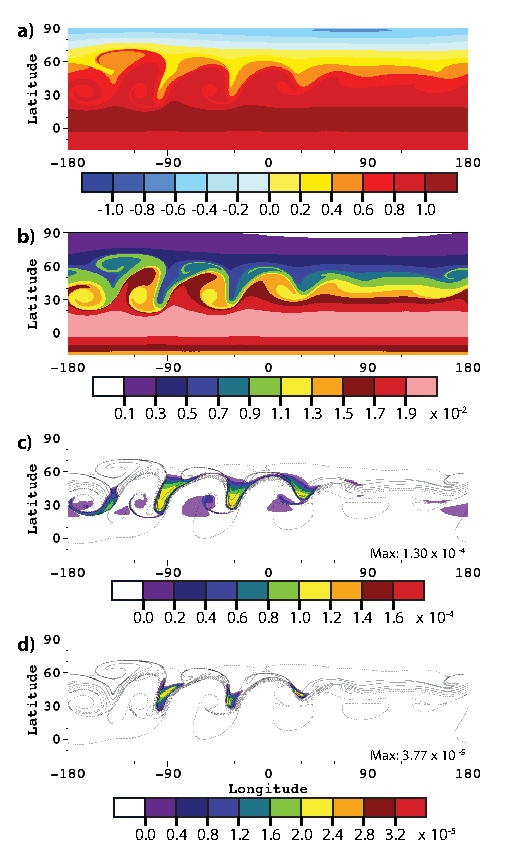
\includegraphics[height=.9\textheight]{Chap2/A_c2048_allvar-01}}
   \caption{Day 6 snapshots of the evolving barotropic wave for the c2048 uniform 
   run's (a) temperature field, (b) $q_v$ moisture field, (c) $q_c$ cloud field, (d) past 12-hour 
   accumulation of the $q_r$ precipitated water field. The solid and dashed black contour
   lines in (c) and (d) represent the positive and negative relative vorticity respectively.
   The spacing between contour lines is $5 \times 10^{-5}$ s$^{-1}$.
   }
   \label{fig:c2048allvar}
\end{figure}

The effects of resolution and variable refinement on the barotropic instability's vorticity
field has been well covered (see \cite{st2007comparison}, \cite{Weller:2009gl}, 
and \cite{scott2016test}). So, we focus our investigation on how the cloud $q_c$ and precipitation of the physics scheme are affected by changing resolution
and AMR. The $q_c$ fields at day 6 for four other uniform resolutions, c128, c256, c512, and
c1024, are depicted in Fig. \ref{fig:uniformqc} for comparison with the c2048 run $q_c$ plot 
in Fig. \ref{fig:c2048allvar}c. The accumulation of precipitated water $q_r$ over
a half day period before day 6 for the four uniform resolutions is plotted in Fig. \ref{fig:uniformqrdt}
and corresponds to Fig. \ref{fig:c2048allvar}d for the uniform c2048 run.

\begin{figure}
   \centerline{%
   \noindent
   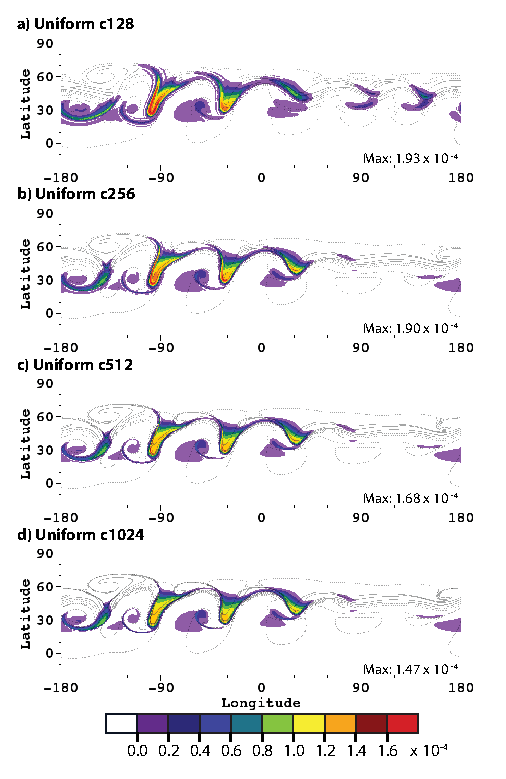
\includegraphics[height=.9\textheight]{Chap2/A_qc_uniform-01}}
   \caption{Plots of the $q_c$ cloud field at day 6 for several 
   uniform resolutions: (a) c128, (b) c256, (c) c512, and (d) c1024.The c2048 uniform run
   plot of the same field in Fig. \ref{fig:c2048allvar}c serves as a reference. 
   The solid and dashed black contour
   lines represent the positive and negative relative vorticity respectively using the
   same contour spacing as in Fig. \ref{fig:c2048allvar}.
   }
   \label{fig:uniformqc}
\end{figure}

\begin{figure}
   \centerline{%
   \noindent
   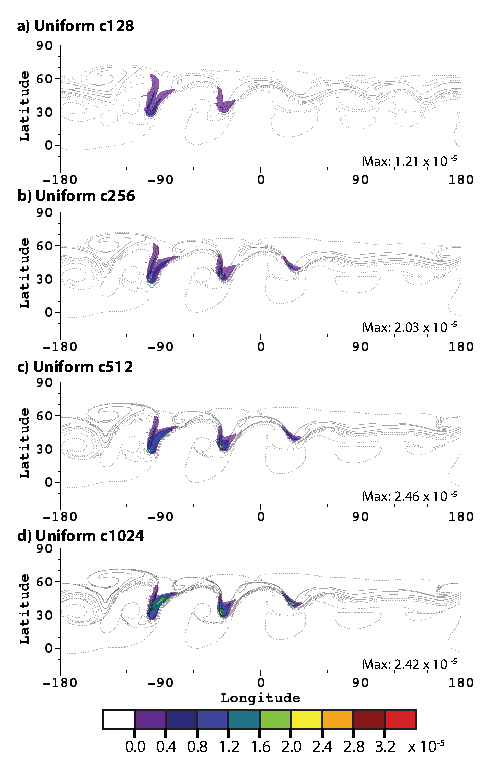
\includegraphics[height=.9\textheight]{Chap2/A_qrdt_uniform-01}}
   \caption{Plots depicting the 12-hour accumulation in the $q_r$ precipitated water field for
   (a) c128, (b) c256, (c) c512, and (d) c1024 uniform runs. The c2048 uniform run
   plot of the same field in Fig. \ref{fig:c2048allvar}d serves as a reference.
   The solid and dashed black contour
   lines represent the positive and negative relative vorticity respectively using the
   same contour spacing as in Fig. \ref{fig:c2048allvar}.
      }
   \label{fig:uniformqrdt}
\end{figure}

Cloud cover area is fairly consistent across all resolutions in Fig. \ref{fig:uniformqc}.
The structure of the cloud field and smaller scale features centered on the cutoff 
lows and the leftmost wave converge at resolutions of c512 and higher. A key
difference in cloud cover structure is in the c128 run in Fig. \ref{fig:uniformqc}a.
The c128 run has two extra areas of cloud cover between $80^\circ$ and
$170^\circ$ longitude, which we interpret as artifacts of the cubed-sphere grid.
As observed by \cite{st2007comparison} and \cite{ullrich:2010vn}, the barotropic
test case provides some difficulties for the cubed sphere. As the jet moves over the four corners of the cubed-sphere, coarser resolution runs generate a wave number
four forcing which affects the development of the solution. In the c256 run (Fig. \ref{fig:uniformqc}b) 
the artifact has disappeared.

While the overall shape and area of the cloud field converges, the concentration
of the $q_c$ field continues to decrease with increasing resolution.
The ribbon-like area of peak cloud concentrations on the edges of the two main troughs
seen in Figs. \ref{fig:uniformqc}a and b are not present in the higher resolution c1024
(Fig. \ref{fig:uniformqc}d) and c2048 (Fig. \ref{fig:c2048allvar}c) runs. In the
plots of 12-hour precipitation accumulation in Fig. \ref{fig:uniformqrdt}, we
observe the opposite trend with the maximum amount of precipitation accumulation 
nearly doubling between the c256 run (Fig. \ref{fig:uniformqrdt}b) and the
c2048 run (Fig. \ref{fig:c2048allvar}d). Like the $q_c$ field, the overall coverage and 
structure of the rain field converges well with resolution, with only the area of 
heavier precipitation expanding as resolution increases. One key feature that
shifts with increased resolution is the area of highest precipitation 
in the front-like system centered around $-90^\circ$ longitude. In the day 6 
precipitation plots for the c256 (Fig. \ref{fig:uniformqrdt}b) and c512 
(Fig. \ref{fig:uniformqrdt}c) runs, the highest levels of accumulation
are concentrated in a small area at the western edge of the bottom
of the trough. In the higher resolution c1204 (Fig. \ref{fig:uniformqrdt}d)
and c2048 runs (Fig. \ref{fig:c2048allvar}d), the areas of most accumulation 
change to a broad area along the leading (eastern) edge and
a secondary long and narrow area along the western edge.

\subsection{The moist barotropic instability with AMR}
  For our implementation of AMR in this moist shallow water
system, we created three refinement tagging criteria. In addition to
the previously used relative vorticity thresholds, two criteria based
on the physics variable $q_c$ are used. The first $q_c$ based criterion is a 
simple threshold of $q_c > 3.0 \times 10^{-5}$. The second cloud based 
criterion is designed to track the leading edges of cloudy areas and is based on the relative gradient of $q_c$. 
Its threshold is $|\nabla q_c| > 7.5\times 10^{-8}$ m$^{-1}$.
The simple relative vorticity threshold is $|\zeta| > 2.3 \times 10^{-5}$ s$^{-1}$.

\begin{figure}
   \centerline{%
   \noindent
   \includegraphics[height=.75\textheight]{Chap2/A_amr_qc-01}}
   \caption{The cloud $q_c$ field profile at day 6 for several AMR runs.  The left column overlays
   the $q_c$ variable with the block structures of the refinement levels in black, while the right columns
   removes these AMR blocks so that the $q_c$ field can be viewed more clearly. 
  (a) - (e) depict AMR runs with one level of x4 refinement while (f) depicts an AMR run with two levels
  of x4 refinement. The tagging criterion for (a), (e), and (f) is a relative vorticity threshold of
  $|\zeta| > 2.3 \times 10^{-5}$ s$^{-1}$. The criterion for (b) and (c) is $q_c > 3.0\times 10^{-5}$,
  and the criterions for the AMR run in (d) is $|\nabla q_c | > 7.5\times 10^{-8}$ km$^{-1}$.
   }
   \label{fig:amrqc}
\end{figure}
%The AMR runs
%   depicted are (a) c64/c256 with a relative vorticity tag, (b) c128/c512 with a $q_c$ magnitude tag,
%   (c) c256/c1024 with a $q_c$ magnitude tag, (d) c256/c1024 with a tag based on the gradient of the
%   $q_c$ field, (e) c256/c1024 with a relative vorticity tag, and (f) c128/c512/c2048 with a relative vorticity tag

Figure \ref{fig:amrqc} shows the $q_c$ field at day 6 for six AMR runs using the three
AMR tagging criteria stated above. The left column in Fig.  \ref{fig:amrqc} shows the
cloud field overlaid with the block structure of the AMR levels, while the right removes
them for easier viewing of the cloud field. 
At coarser resolutions, AMR runs using the $q_c$ tagging criteria have only small 
areas of refinement in place after day 4. This still allows 
the grid imprinting to develop as seen in Fig. \ref{fig:amrqc}b, the c128 base resolution
1-level AMR run with the $q_c$ threshold tag. Additionally, while the two
heaviest cloud areas compare well their counterparts in the uniform c512 run (Fig. \ref{fig:uniformqc}c),
the two weaker areas of clouds centered around $-170^\circ$ longitude
and $30^\circ$ longitude more closely resemble the uniform c128 run (Fig. \ref{fig:uniformqc}a)
The vorticity tagging
criterion used for the c64 base resolution AMR run in Fig. \ref{fig:amrqc}a places higher resolution 
at the start of the simulation over the entire jet, which prevents grid imprinting.
As a result of the larger area of refinement, this c64 AMR run achieves a similar result to the
uniform c256 run (Fig. \ref{fig:uniformqc}b). 

For the c256 base resolution AMR runs with one-level of x4 refinement
in Figs. \ref{fig:amrqc}c, d, and e, as well as the c128 base resolution two-level x4 
refinement AMR run in Fig. \ref{fig:amrqc}f, the resolution over the jet is high enough
to avoid the wavenumber four grid imprinting. The $q_c$ fields for the
 three c256 base resolution AMR runs visually converge to the uniform c1024 run,
 albeit with some poorly resolved rings of low concentration along the edges of the main $q_c$ areas
 in the two AMR runs using the $q_c$ value and $q_c$ gradient tags. This structure
corresponds to the coarse-fine grid boundary, though it is caused by a response to the increased
resolution rather than a computational artifact of the grid itself.
In the c128 and c256 uniform runs, the main filaments of cloud in Figs. \ref{fig:uniformqc}a and b
are buttressed by thin parallel low density cloud filaments. These secondary filaments are either reduced 
in size or no longer present in the higher resolution uniform runs. In the AMR runs, the coarse-fine
boundary intersects these secondary filaments, causing the patchwork pattern seen in
Fig. \ref{fig:amrqc}b, c, and d. It is less pronounced in Fig. \ref{fig:amrqc}e because the vorticity 
tagging threshold triggers refinement over a broader area, providing a buffer-like effect. The c128 two-level
AMR run with vorticity tagging has a highest refinement level of c2048 over most of the jet for the duration of
the model run time. Its $q_c$ field at day 6, seen in Fig. \ref{fig:amrqc}f, depicts levels of cloud 
concentration (denoted by the orange and yellow contours) which are more comparable to the uniform c1024 run.
 
 \begin{figure}
   \centerline{%
   \noindent
   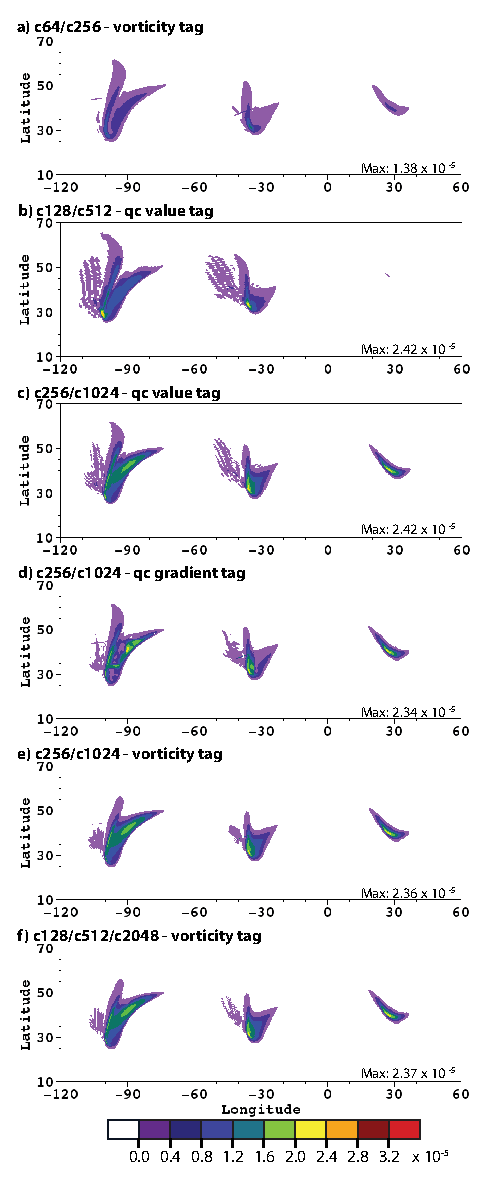
\includegraphics[height=.75\textheight]{Chap2/A_amr_qrdt_zoom-01}}
   \caption{Past 12-hour accumulation of $q_r$ at day 6 for the AMR runs depicted in Fig. \ref{fig:amrqc}.
   }
   \label{fig:amrqrdt}
\end{figure}

The same comparison to uniform runs can be made for the 12 hour $q_r$ accumulation
at day 6 of the six AMR runs pictured in Fig. \ref{fig:amrqrdt}. The AMR grid structure is the same
as in Fig. \ref{fig:amrqc}, so the block structure is not shown in these plots. The overall structure
of the accumulation compares to uniform runs for the $q_c$ field.
The area and magnitude of heaviest accumulation correspond well to the uniform resolution runs,
with the same resolution as the highest resolution AMR runs; the c128 1-level AMR run
in Fig. \ref{fig:amrqrdt}f is again more similar to the uniform c1024 run rather than the c2048 run.
One key difference is observed in the 
c256 AMR run tagging on $q_c$ gradient in Fig. \ref{fig:amrqrdt}d. For this AMR run, the
 area of higher accumulation on the eastern side of the front
system, centered near $-90^\circ$ longitude,
is disjointed and compressed compared to the larger and smoother structure of accumulation in
the corresponding c1024 uniform run in Fig. \ref{fig:uniformqc}d.
With the $q_c$ gradient tagging, the interior areas of the large troughs have no high resolution refinement. 
This results in this precipitation accumulation structure observed 
as the coarser resolution has lower levels of accumulation.
Another contrast is seen in the c128 and c256 AMR runs, which have large areas of low-level accumulation noise 
on the western sides of the two largest troughs. The noise is most pronounced in the three
$q_c$ tagging runs (Figs. \ref{fig:amrqrdt}b,c, and d), though present over a smaller area in vorticity tagging runs, 
specifically Fig. \ref{fig:amrqrdt}e and f. A lower cloud concentration threshold may reduce the noisy low-level edges, extending refinement out beyond the cloud formation areas.


%%%%%%%%%%%%%%%
\section{Conclusion}
\label{sec:conclusion2}
We implemented two different forcing schemes designed to 
mimic the effects of moisture in the atmosphere within a 2D 
shallow water system in a fourth-order finite-volume model
that is adaptive in both space and time. The first moist physics
framework adds a water vapor variable and models convection
as a mass sink triggered by saturation. We implemented a
strengthening vortex test case with this setup.  In the second
forcing framework, a more complex moisture representation
is used, consisting of vapor, cloud, and rain variables.
The effects of moisture were coupled to the momentum equations
through a potential temperature variable, linked to
the moisture variables through latent heat. The model used
this setup with the barotropic instability test case. 
With both forcing systems and test cases, we observe
the evolution of features of interest at various resolutions and 
with differential refinement strategies. 
We also investigate AMR's effect on the physics 
forcing as grid resolutions changed.
These simulations can aid the
establishment of guidelines for effective AMR refinement criteria.

The resolution
dependency of the physics forcing schemes were relatively mild.
In the Kessler-like
moisture scheme with the barotropic instability test, 
the overall structure of the moisture variables converged quickly
with increasing resolution, though the concentration of clouds and
precipitation accumulation continued to change with resolution. In
the convective vortex forcing setup, we observed a resolution-dependent
two-regime vortex evolution structure. For resolutions c512 and greater,
we observed a convergence of vortex's shape and structure. Though
the maximum wind speed and relative
vorticity continued to slowly increase with resolution.
The forcing in both cases functioned effectively across the varying
resolutions and multiple levels of AMR. The coarse-fine interfaces
did not induce noise or significant distortion 

The sensitivity to resolution and AMR refinement criteria was much
more pronounced in the strengthened vortex setup.
The response of the moist barotropic wave test case to 
AMR refinement criteria was fairly consistent; changes in criteria
did not significantly alter the growth and structure of clouds and rain within the wave,
so long as the initial refinement adequately resolved the wave to avoid
computational grid artifacts. Any additional refinement was effective.
In the strengthening vortex test case, the strength and evolution 
of the central vortex ring were quite sensitive to initial resolution and the time point at which
AMR levels are triggered. Though the vortex does not strengthen 
significantly or undergo rapid structural changes during the first few days, 
we observed that AMR runs with solutions most similar to the uniform high
resolution runs had some initial levels of refinement either initially (at least c256) or within
the first day (at least c512). The vortices in these runs evolved at a comparable rate
and strength to those in the uniform run with the same resolution
as the highest AMR level, even if that level was not triggered until several days later.
AMR not added initially was still beneficial.
Once sufficient resolution was triggered, the vortex underwent the process of 
rapid strengthening, collapsing, and reforming. The high resolution vortex evolution process was merely delayed by lack of refinement. 
The application of refinement allowed the vortex to catch-up to the high resolution reference vortex.
The time window in which AMR would trigger this process was limited.
If high resolution AMR was not triggered until many days into the simulation, 
the AMR solution diverged from the high resolution runs.

Both sets of simulations show the starting grid resolution must be
able to adequately resolve the features of interest to maximize
AMR effectiveness. AMR cannot remove the errors
caused before refinement begins. Additional refinement with
AMR beyond that base level did improve the model, especially
with regards to the small scale vorticity features in the strengthen vortex.
To obtain this early refinement with AMR, the tagging
criteria must be tailored to properties uniquely associated
with the origins of the feature of interest, which is difficult even in these 
idealized shallow water systems, or must use a combination of initial static refinement 
and AMR. For example, in tracking and resolving TCs in a realistic climate simulation, a static region of refinement
could be placed over regions of cyclogenesis. Any storms that
develop could be further refined with AMR tagging on
surface pressure and followed as they traverse
and exit the region of static refinement.
Future work will consist of extending the analysis
to AMR in the full 3D dycore, focusing on
similarly simplified physics parameterization schemes.

 
 \chapter{Implementing AMR in the 3D dynamical core with dry and simple physics test cases}
 \label{chap:3dmodel}
 \section{Introduction}
Variable resolution grids have been used in regional atmospheric models for several decades
\citep{fox1997finite}. The most common downscaling approach was the nested grid, in which
a fixed-size refined grid is embedded within the coarse grid at a set location. It was implemented in several
limited area models (LAM) for local weather forecasting
and regional climate simulations (e.g. \cite{Phillips1979nested}, \cite{pielke1992comprehensive}, \cite{grell1994description},
and \cite{caya1999semi}). Many of these models are regularly used today.
For example, one of the most frequently used LAMs with embedded nested grids is the
Weather Research and Forecasting Model (WRF, \cite{Skamarock:2008db}).

An alternative approach to downscaling designed for global 
models is the stretched grid that was developed
around the same time \citep{Schmidt:1977qo, staniforth1978variable}. 
In these models, an originally
uniform mesh is smoothly distorted such that more grid elements are concentrated
over a localized region, providing higher resolution in that area and leaving 
fewer grid elements, and thus coarser resolution, 
in the remaining area. Stretched grids require few modifications to the
numerical schemes and computational grids to implement in general circulation models (GCMs). 
Thus they were an attractive technique to 
implemented in variable resolution modeling because GCMs avoid many drawbacks 
associated with LAMs such as lateral boundary conditions and their inability
to capture upscaling effects. Several stretched grid models developed
at that time include \cite{paegle1989variable}, \cite{deque1995high},
\cite{yessad1996introduction}, \cite{fox1997finite}, and \cite{cote1998operational}).

Early
GCMs using nested grids were developed by \cite{Ruge:1995cy} and \cite{dudhia2002global}.
Nested grids within GCMs involve continuous two-way 
communication between resolutions and require more challenging numerical
schemes and computational grids.
This made them initially less attractive in comparison to stretched grids. 
A second form of nesting involves a single grid spanning multiple resolutions, where refined
grid cells physically replace the coarse cells in the region of interests.
An early example of this technique was implemented by \cite{Fournier:2004cf}.

With the advancement of large-scale parallel computing systems,
variable resolution GCMs are
a growing fixture in atmospheric and climate modeling. Variable resolution has been 
incorporated into several operational GCMs across major modeling centers 
\citep{skamarock2012multiscale,Harris:2013nt,zarzycki2014aquaplanet}.
This combination has proven to be effective for assessing
tropical cyclones \citep{zarzycki2014multidecadal, zarzycki2015tropical, huang2017influences}, 
large-scale weather systems \citep{rauscher2014impact}, atmospheric rivers \citep{hagos2015resolution},
 and regional climate \citep{medvigy2013simulated, huang:16, gettelman2017regional, rhoades2018projecting}.
Specifically, variable resolution can bridge the difference in 
scale between global and regional climate modeling by overcoming
many of the known issues with conventional downscaling methods of LAMs or high resolution GCMs.
They provide high-resolution in a desired location while eliminating the need for forced lateral boundary conditions, 
capture small-to-large scale teleconnections, and demand fewer computational
resources compared to standard uniform high-resolution GCMs.

The variable resolution models discussed thus far implement static grid refinement.
The refined grid's location is determined \emph{a priori} and remains fixed for
the entirety of the simulation. Dynamic grid refinement, such as adaptive mesh refinement (AMR),
is a more flexible variable resolution modeling technique. Adaptive grids track features of interest
and refine the grid locally in advance of any important physical features or processes requiring
additional resolution. When the additional resolution is no longer needed, that same region of
the grid is coarsened.
While dynamic refinement is frequently implemented in other areas of computational 
hydrodynamics such as aerospace and heliophysics, it has not been widely adapted
for atmospheric and climate modeling. Since dynamically adaptive grids were first
applied to atmospheric flows by \cite{skamarock1989adaptive},
\cite{skamarock1993adaptive} and \cite{Dietachmayer:1992sj}, adaptive model
work has been limited to algorithm development, simplified models, and idealized simulations.
Dynamically adaptive shallow water models on the sphere have been discussed in
\cite{giraldo2000lagrange}, \cite{behrens2005amatos}, \cite{lauter2007parallel}, 
\cite{st2007comparison}, \cite{kubatko2009dynamic}, and \cite{Chen:2011kk}.
More recent model designs have been presented in \cite{mccorquodale2015adaptive},
\cite{tumolo2015semi}, \cite{aechtner2015conservative}, and \cite{weller2016mesh}.
Several applications of AMR and dynamic refinement in the shallow water system 
include tsunami propagation in \cite{blaise2012dynamic}, Fujiwhara interactions in
\cite{bauer2014simulation}, and tropical cyclone eye-wall evolution in
\cite{hendricks2016evaluation}. \cite{ferguson2016analyzing} provides
more detailed overview of these models and their dynamic refinement techniques.
 Though some LAM models like 
WRF \citep{shepherd2017sensitivity} have primitive 
moving nested grids, these cannot be considered true AMR models. 
The nests in these models are often fixed in size and grid elements cannot 
be added or removed. The only full 
3D atmospheric model with dynamic refinement known is the OMEGA
model by \cite{bacon2000dynamically}. This adaptive non-hydrostatic limited-area model
implemented on rotated Cartesian coordinates has been used as a regional hurricane
forecasting system in \cite{gopalakrishnan2002operational}.

This chapter explores the use of mapped-multiblock AMR techniques for three-dimensional 
atmospheric flows. We use the nonhydrostatic finite-volume Chombo
AMR model on the cubed-sphere extended to the full 3D atmospheric equations from the 
2D shallow water model of \cite{mccorquodale2015adaptive}. We wish to
characterize the ability of this model and its multiblock refinement
to simulate atmospheric flow in the global 3D system. To this end, we 
implement the \cite{lin2017colliding} modon test case in the dynamical core (dycore) without any
forcing or subgrid physical parameterization. We run convergence tests and 
demonstrate the use of AMR with simple tagging criteria to observe how
effectively AMR resolves and tracks the modons. We also implement a second
test case, the idealized tropical cyclone from \cite{reed2011vortex}, in which a single,
idealized initial weak vortex evolves into a tropical cyclone. This test requires
the simplified physics scheme from \cite{reed2012idealized} consisting of parameterizations for large-scale condensation,
boundary layer diffusion, and surface fluxes for moisture, sensible heat, and
momentum. With the idealized vortex, we investigate the AMR's ability to track and resolve
the strengthening cyclone using various refinement criteria and thresholds to trigger 
refinement. The results presented are an preliminary assessment of
the AMR capabilities of the 3D models. This model is still undergoing development and
we are currently discovering, evaluating, and resolving instabilities. Several of these issues are noted in
following sections.

This chapter proceeds as follows. Section \ref{sec:experimental} contains a brief description of the 
the nonhydrostatic 3D finite-volume model on the cubed-sphere.
In section \ref{sec:modon}, we present the results of the colliding modon test,
including convergence tests.  The results of
the idealized tropical cyclone test and the comparisons of
various AMR refinement criteria are discussed in section \ref{sec:tctest}. In Section
\ref{sec:conclusion3} we summarize our conclusions and comment on the direction of future
research.

\section{Experimental design}
\label{sec:experimental}

The non-hydrostatic finite-volume Chombo AMR model
is a global 3D model built upon the shallow water version presented in \cite{mccorquodale2015adaptive}.
The dycore utilizes the full-non-hydrostatic moist fluid equations in a shallow-atmosphere
approximation on a cubed-sphere grid.

\subsection{Cubed-Sphere Grid}
The cubed-sphere grid, first developed by \cite{sadourny1972conservative}, consists of a cube with six Cartesian panels inflated out to form a spherical shell.
The grid avoids this pole-problem of traditional latitude-longitude grids by replacing the two strong singularities at the poles with eight weaker singularities at
the corner points of the originally cube. The cubed-sphere grid also provides a near uniform tiling of the sphere as compared to
large changes in grid spacing on the latitude-longitude mesh. 
There are multiple ways to map the grids of each panel to the sphere (see \cite{putman2007finite} for a review
of several cubed sphere grids).  The Chombo-AMR model uses gnomonic equiangular cubed-sphere grid, where the
gridlines on each panel have equally spaced central angles relative to the center of the sphere. This projection
yields a quasi-uniform spherical grid. The grid does not have perfectly uniform tile sizes, but as resolution increases
the ratio between the largest and smallest grid cells converges to $\sqrt{2}$, the smallest ratio of cubed-sphere
grids. Figure \ref{fig:cubedsphere2dmaps} depicts the equiangular cubed-sphere grid.

\begin{figure}[htp]
\centerline{
\includegraphics[width=4in]{Chap3/cubedsphere12456.pdf}                                                                                        
}
\caption{
A cubed-sphere grid, shown with labels on panels.                                                                                                             
Panels 1 -- 4 all straddle the equator
($z = 0$) of the unit sphere.
Panel 5 is centered on the north pole ($z = +1$),
panel 6 on the south pole ($z = -1$).
On the cubed-sphere grid shown here,
$N_{\rm c} = 16$ (each panel contains $16 \times 16$ grid cells).
}
\label{fig:cubedsphere2dmaps}
\end{figure}

The physical domain of the model 
is a spherical shell $r \in [R_i,R_f]$ with a thickness of $H = (R_f - R_i)$,
where $R_i$ and $R_f$ are the radii of the model 
bottom and top respectively, and the assumption 
that $H \ll R_i, R_f$. This shallow 
atmosphere assumption allows us to neglect $r$ metric
dependencies (e.g. no area increase with altitude).
The physical domain is mapped from the cubed-sphere grid.

The equiangular coordinates system for the 
cubed-sphere grid is given as $(\alpha, \beta, \xi, n_p)$, defined
on six panels $n_p \in [1,2,\dots, 6]$, with central angles $\alpha, \beta \in [-\frac{\pi}{4},\frac{\pi}{4}]$ and 
vertical coordinate $\xi \in [0,1]$. By convention, panels 1-4 are along the 
equator and panels 5 and 6 are centered on the north and south poles,
respectively, as seen in Fig. \ref{fig:cubedsphere2dmaps}. 
Each panel is discretized into an $N_c \times N_c$ grid of quadrilaterals.
The edges of each grid cell are non-orthogonal 
segments of the great circle in either the $\alpha$ or $\beta$ direction. 
This property makes the computational grid sizes constant so that
$d\alpha = d\beta = \frac{\pi}{2N_c}$. 
The discrete horizontal resolution of the cubed-sphere grid is represented as  $c\{N_c\}$.
A list of the horizontal properties of the equiangular cubed-sphere grid, including the
approximate grid spacings, and comparable resolutions for other coordinate systems, is given in
Table~\ref{tb:grids} for several resolutions.

The vertical direction is discretized into $N_v$ layers 
with non-constant thickness but constant thickness in the 
computational domain so that for each level $\Delta \xi = 1/N_v$.
The mapping $r(\xi)$ between the physical and computational 
domains is such that
$r(\xi=0) = R_a$ and $r(\xi=1) = R_a + H$ where $R_a$ is the radius of 
the spherical shell and $H$ is the height of the model top. 
The height-based vertical mapping is set by a user-created 
array consisting of the coordinate positions for the vertical level interfaces in physical space.
For non-uniformly spaced vertical maps, the final positioning of the 
level interface points are smoothed via a cubic spline.


\subsection{Fluid equations in cubed-sphere coordinates}
The dycore utilizes the following state variables
\begin{equation}
\label{eq:imexsplit}
\bS
  = 
\begin{bmatrix}
  \avg{J \rho \ua} \\
  \avg{J \rho \ub} \\
  [w]_f \\
  [p]_c \\
  \avg{J \rho} \\
  \avg{J \rhoth} \\
  \avg{J \rhoqv} 
\end{bmatrix}.
\end{equation}
Angled brackets $\avg{}$ indicate a cell averaged variable for the density $\rho$, the horizontal 
momentum density variables $\rho \ua$ and $\rho \ub$ in the $\alpha$ and
 $\beta$ directions on the cubed-sphere, respectively.
The virtual potential temperature is $\theta_v$ and the 
specific humidity $q_v$ which will serves as a placeholder for other physics tracers. 
Vertical velocity $w$ is face-centered variable indicated by $[]_f$ and 
pressure $p$ is a cell-centered variable, indicated by $[]_c$.
$J$ is the metric Jacobian.
The relationship
between the physical vertical velocity $w$ and the computational vertical velocity $\uxi$ 
is given by
\begin{equation}
w = r_{\xi}\uxi.
\end{equation}
The relationship between the derivates in the computational 
vertical coordinate $\xi$ and physical vertical coordinate $r$
is
\begin{equation}
  \partial_r = r_{\xi}^{-1} \partial_{\xi}.
\end{equation}
In both equations, $r_{\xi}$ is the vertical coordinate transform term for converting
between physical and computational spaces.
The virtual potential temperature is defined as
\begin{equation}
\theta_v = (1-0.61q_v)T\left(\frac{p_0}{p}\right)^\kappa,
\end{equation}
where $T$ denotes the temperature, $p_0=10^5$ Pa is the reference pressure and $\kappa = R_d /c_{pd}$.
Here $R_d$ is the ideal gas constant and $c_{pd}$ is the specific heat at constant 
pressure, both in the case of dry air.

With these variables the equations of motion in conservation form on the cubed sphere grid are:
\begin{align}
\frac{\partial J \rho \ua}{\partial t} &=  - \sum_{i=\alpha, \beta} \partial_i (J \rho \ua u^i + JG^{\alpha i} p )
    - \dxi (J \rho \ua \uxi + JG^{\alpha \xi} p)  + J \Psi_C^\alpha + J \Psi_M^\alpha\\
\frac{\partial J \rho \ub}{\partial t} &=  - \sum_{i=\alpha, \beta} \partial_i (J \rho \ub u^i + JG^{\beta i} p )
    - \dxi (J \rho \ub \uxi + JG^{\beta \xi} p)
    + J \Psi_C^\beta + J \Psi_M^\beta \\
\frac{ \partial w}{\partial t} &=   - \sum_{i=\alpha, \beta} u^i \partial_i w - \uxi \, \dxi w - \frac{1}{\rho} \dr p - g \\
\frac{\partial p}{\partial t} &=   - \sum_{i=\alpha, \beta} \left( \gamma p \frac{1}{J} \partial_i (J u^i) 
    + u^i \partial_i p \right) - \uxi \dxi p  - \gamma p \, \dr w  + \eta \left(P(\rhoth) -p \right) \label{eq:eompress}\\
\frac{ \partial J \rho}{\partial t} &=  - \sum_{i=\alpha, \beta} \partial_i (J \rho u^i) - \dxi ( J \rho \uxi ) \\
\frac{ \partial J \rhoth}{\partial t} &=  - \sum_{i=\alpha, \beta} \partial_i (J \rhoth u^i) - \dxi ( J \rhoth \uxi ) \\
\frac{ \partial J \rhoqv}{\partial t} &=  - \sum_{i=\alpha, \beta} \partial_i (J \rhoqv u^i) - \dxi ( J \rhoqv \uxi )
\end{align}
where $G^{ij}$ represent the contravariant cubed-sphere metric term, $g$ is the acceleration
due to gravity, and $\gamma = 1 / (1 - \kappa)$. $\Psi_C$ and $\Psi_M$ represent source terms
from the Coriolis force and metric terms due to the cubed-sphere geometry, respectively. 
These source terms and coordinate transforms that arise from using cubed-sphere mapping may be found in
Appendices A and B of \cite{ullrich2012mcore}.
Currently no topography is implemented. 
Finally the moist equation of state for the equations of motion is
\begin{equation}
\label{eq:eos}
P = p_0\left(\frac{R_d\rhoth}{p_0}\right)^\gamma.
\end{equation}

Equation \ref{eq:eompress} includes a volume discrepancy term: $\eta \left(P(\rhoth) -p \right)$ 
with relaxation parameter $\eta = 0.5 $ to prevent the 
prognostic pressure $p$ from drifting from the equation of state pressure $P$. 
The volume discrepancy approach is used in gas dynamics 
modeling to couple non-linear explicit flow solvers and stiff 
reactions and to maintain conservation in potential 
temperature density \citep{day2000numerical}. Because the equations
of motion are closed with the equation of state Eq. \ref{eq:eos}, this leads to a non-linearity in
$\theta_v$ which leads to pressure values drifting apart. Note that the redundant pressure equation
makes it convenient to treat acoustic waves implicitly. 
The volume discrepancy term relaxes the prognostic pressure to the equation of state pressure.

\subsection{Numerical Methods}
The non-hydrostatic equations are spatially discretized with a finite-volume scheme 
that was implemented by \cite{mccorquodale2015adaptive} for the shallow water equations.
The 3D scheme computes the horizontal fluxes with fourth-order accuracy, but is only accurate
to second-order in the vertical.  To perform the finite volume calculations on panel edges, the 
mapped-multiblock approach creates three layers of ghost cells 
and remaps the values from neighboring cells to these ghost cells. 
 In addition, a sixth-order diffusive operator which maintains the fourth-order 
 accuracy of the scheme is applied to the horizontal fluxes. 
There is no dissipation in the vertical. The numerical scheme is 
mass-conserving to machine precision and energy-conserving up to the
temporal truncation order, when used without limiters or explicit
dissipation. Since topography is not yet mplemented in the dycore, 
simple height-based vertical coordinates are used.

Time integration is conducted by an implicit-explicit second-order, three stage 
ARS232 scheme by \cite{ascher1997implicit}. Given the 
large aspect ratio in the vertical direction, vertical acoustic waves, which are supported by
the shallow atmosphere equations of motion, would severely limit the global time step.
Thus, the terms responsible for vertical acoustic waves in the $w$ and $p$ equations are separated out to
be treated implicitly. All the horizontal terms and the remaining advection terms for the vertical
variables are evaluated explicitly.

The mapped-multiblock AMR techniques developed from the Chombo library \citep{Adams:2015gd} 
and used for the shallow water model in \cite{mccorquodale2015adaptive} and \cite{ferguson2016analyzing}
are implemented in the full 3D dycore.
AMR calculations are performed on a hierarchy of nested meshes, called
levels, which have a defined refinement ratio between them. 
The finer levels are overlaid on top of the coarser levels.  Information on these finer
level is initialized via interpolations from the coarser level and ghost cells 
are used to calculated the fluxes at patch boundaries. Information from the finer level
is averaged down to update values on the coarser level.
These levels are sub-cycled in time to maintain a constant Courant
number across all levels. A detailed overview of the AMR level strucutre and
sub-cycling time integration is provided in Chapter \ref{chap:basicsw}.
Refinement is only done in the horizontal direction, vertical refinement is not currently implemented. 
When an AMR level is initialized, refinement is added uniformly throughout all
vertical levels.

Several modifications have been made to achieve a working dycore to present these results.
Refluxing across panel boundaries is currently not implemented so mass conservation is not guaranteed at panel edges
or at coarse-fine boundaries. Additionally, the fourth-order horizontal discretization drops to second order
at panel boundaries, though coarse-fine boundaries are still fourth-order.
A simple clipping limiter is used to prevent moisture variables from going negative. An optional ability to
incorporate Rayleigh damping in the upper atmosphere has also been implemented. 
Rayleigh damping is added as a source term in the form
\begin{equation}
   \Psi_R = -R_c(\alpha,\beta, \xi)\left(\rho\mathbf{u} - \rho\mathbf{u_0}\right),
\end{equation}
where $R_c$ denotes the strength of the damping, $\rho\mathbf{u}$ is the 3D momentum density vector, and $\rho\mathbf{u_0}$ denotes
a reference state for the momentum. For these simulations, $\mathbf{u_0}$ is set to zero. The strength of the damping term
is designed to smoothly transition from zero damping at lower levels to a maximum at the model top. We choose
\begin{align}
   R_c(\alpha,\beta, \xi) = \ & 0 \ &  \mathrm{if} \ \xi < \xi_r, \\
   R_c(\alpha,\beta, \xi) = \  & \frac{1}{\tau_R}\left(\frac{\xi - \xi_r}{1-\xi_r}\right)^2 \ & \mathrm{if} \ \xi > \xi_r.
\end{align}
Here $\tau_R$ is the timescale of the damping and $\xi_R$ is the starting height of the damping layer in $\xi$ coordinates. We use
$\tau_R = 1$ day and $\xi_R = \frac{2}{3}$, which places damping in the upper third of the atmosphere only.
Rayleigh damping is currently not used in the modon simulations
but is activated for the idealized tropical cyclone tests. No additional limiters or filters are
implemented.


\section{Modon test case implemented in the dry dynamical core}
\label{sec:modon}
The \cite{lin2017colliding} colliding modon test consists of two anti-polar pairs of counter-rotating vortices, which are
centered on the equator and overlay a calm, hydrostatic background.
We implement it in a dry version of the dycore for use in some basic convergence studies and a
first look at the efficacy of AMR. The modons are slow-moving, isolated features that can be easily tagged for refinement
with a vorticity threshold. These characteristics make the test case effective for discerning problems that
might arise due to refinement, instabilities due to the numerical schemes, and
 noise or wavelike reflections at AMR boundaries.

\subsection{Initialization and basic characteristics}
Each modon is a dipole of positive and negative vorticity regions on either side of the equator.
In this test case by \cite{lin2017colliding}, two modons are initialized at the equator on opposite sides
of the sphere. The two modons initially undergo rapid cyclostrophic adjustment due to 
unbalanced initial conditions.  This creates a gravity wave which propagates 
around the globe but has no effect on the structure of the modons.
The modons travel slowly (6-7 m/s) towards each other along the equator as 
there is no planetary rotation, until they collide after approximately 22 days. 
The collision creates a modon moving northward and another moving southward. In 
\cite{lin2017colliding} the simulation runs for 100 days,
during which the two modons cross the poles and then collide at the equator on the opposite side, 
exchanging vorticity again. After 100 days they have passed through their initial positions 
and begin the loop again. Without diffusion, the modons should cycle indefinitely. 
However, in realistic models they will slowly decay.  We only run the simulation  
to a maximum of twenty days due to instability issues that cause the modon structure to collapse 
shortly after this time. An additional issue affecting AMR runs is triggered when an 
AMR level intersects a polar panel edge, and the sources of these issues are under investigation.

The modons are initialized in an isothermal temperature profile of $300$K and a pressure 
field that is hydrostatically balanced with an initial surface pressure of 1,000 hPa. 
Uniform vertical height coordinate mapping is utilized with 16 vertical levels, though 
one set of convergence tests are run with 32 vertical levels. 
The model top is set to 10 km.  
There is no moisture in this setup and the Coriolis rotational forcing is not included.
The velocity is zero everywhere except for the initial zonal
wind perturbations of the modons, which is uniform throughout the vertical. The initial zonal wind is
\begin{equation}
\label{eq:modonwind}
  u(\theta,\lambda) =  U_0 \left(\exp{\left(-\left(\frac{r_1}{r_0}\right)^2\right)} - \exp {\left(-\left(\frac{r_2}{r_0}\right)^2\right)}\right)
\end{equation}
where $U_0=40$ m s$^{-1}$, $r_0 =500$ km, $(\theta,\lambda)$ are the latitude and longitude, and $r_1$ and $r_2$ are the
great-circle distance from each modon's center. The modons are initially centered at $(\theta_1,\lambda_1) = (0,\pi/2)$ and
$(\theta_2,\lambda_2) = (0,3\pi/2)$. The vortex structure of the modons can be seen in Fig. \ref{fig:modonvortplot}a.  

\subsection{AMR with the modon test}
We compare the results from a series of uniform and AMR runs to assess
if the AMR correctly tags, refines, and follows the non-linear modons.
We implement one refinement criterion for all AMR runs: 
a relative vorticity threshold of $|\zeta| > 2 \times 10^{-5}$ s$^{-1}$.
Figure \ref{fig:modonvortplot} shows the 5 km height vorticity profiles of 
the uniform c128 (left column) and c32/c128 AMR runs (right column) at
days 0, 10, and 20. At this resolution, the modons lose more than a quarter of 
their strength over the first twenty days; at higher resolutions there is only minimal
loss of strength.
The vorticity tagged refinement in the c32/c128 run successfully
refines the modon areas immediately and is able to track
the propagating modons. The size and intensity 
of the modons in the AMR run are preserved in comparison to the c128 run. 
We can see this more concretely in Fig.
\ref{fig:modontevol} which plots the 10-day time evolution of the 
maximum vorticity of the modons for uniform runs from c64 to c512 and three AMR runs
all using the same $|\zeta| > 2 \times 10^{-5}$ s$^{-1}$ refinement criteria. The uniform runs
show that for coarse resolutions, c128 and below, the modons rapidly decay. For c256 and
higher the modons maintain their intensity. For the three AMR runs: c32/c128,
c64/c256, and c128/c512, we see strong alignment in maximum vorticity to
that of the uniform run with the same resolution as the AMR level. This result is
not surprising as the AMR was in place over the modons for the entire run, but it
does demonstrate that on the panels and across the equatorial panel edges AMR is
functioning as expected.

\begin{figure}
    \centerline{%
    \noindent
    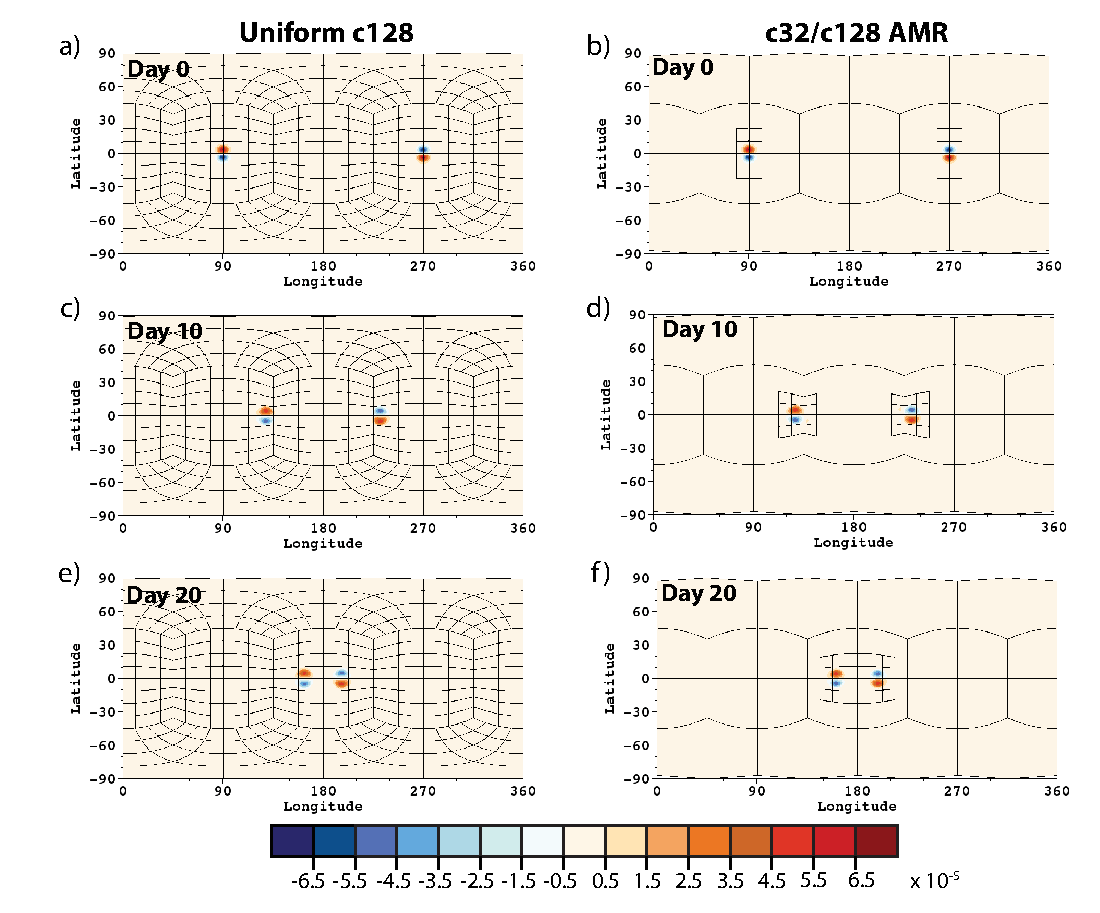
\includegraphics[width=\textwidth]{Chap3/modon_vortex_compare-01.eps}}
    \caption{Snapshots of the vorticity field at day 0 (a)-(b), day 10 (c)-(d),
    and day 20 (e)-(f) for a uniform c128 run (left column) and a c32/c128 AMR
    run (right column).
}%
    \label{fig:modonvortplot}
\end{figure}

\begin{figure}
    \centerline{%
    \noindent
    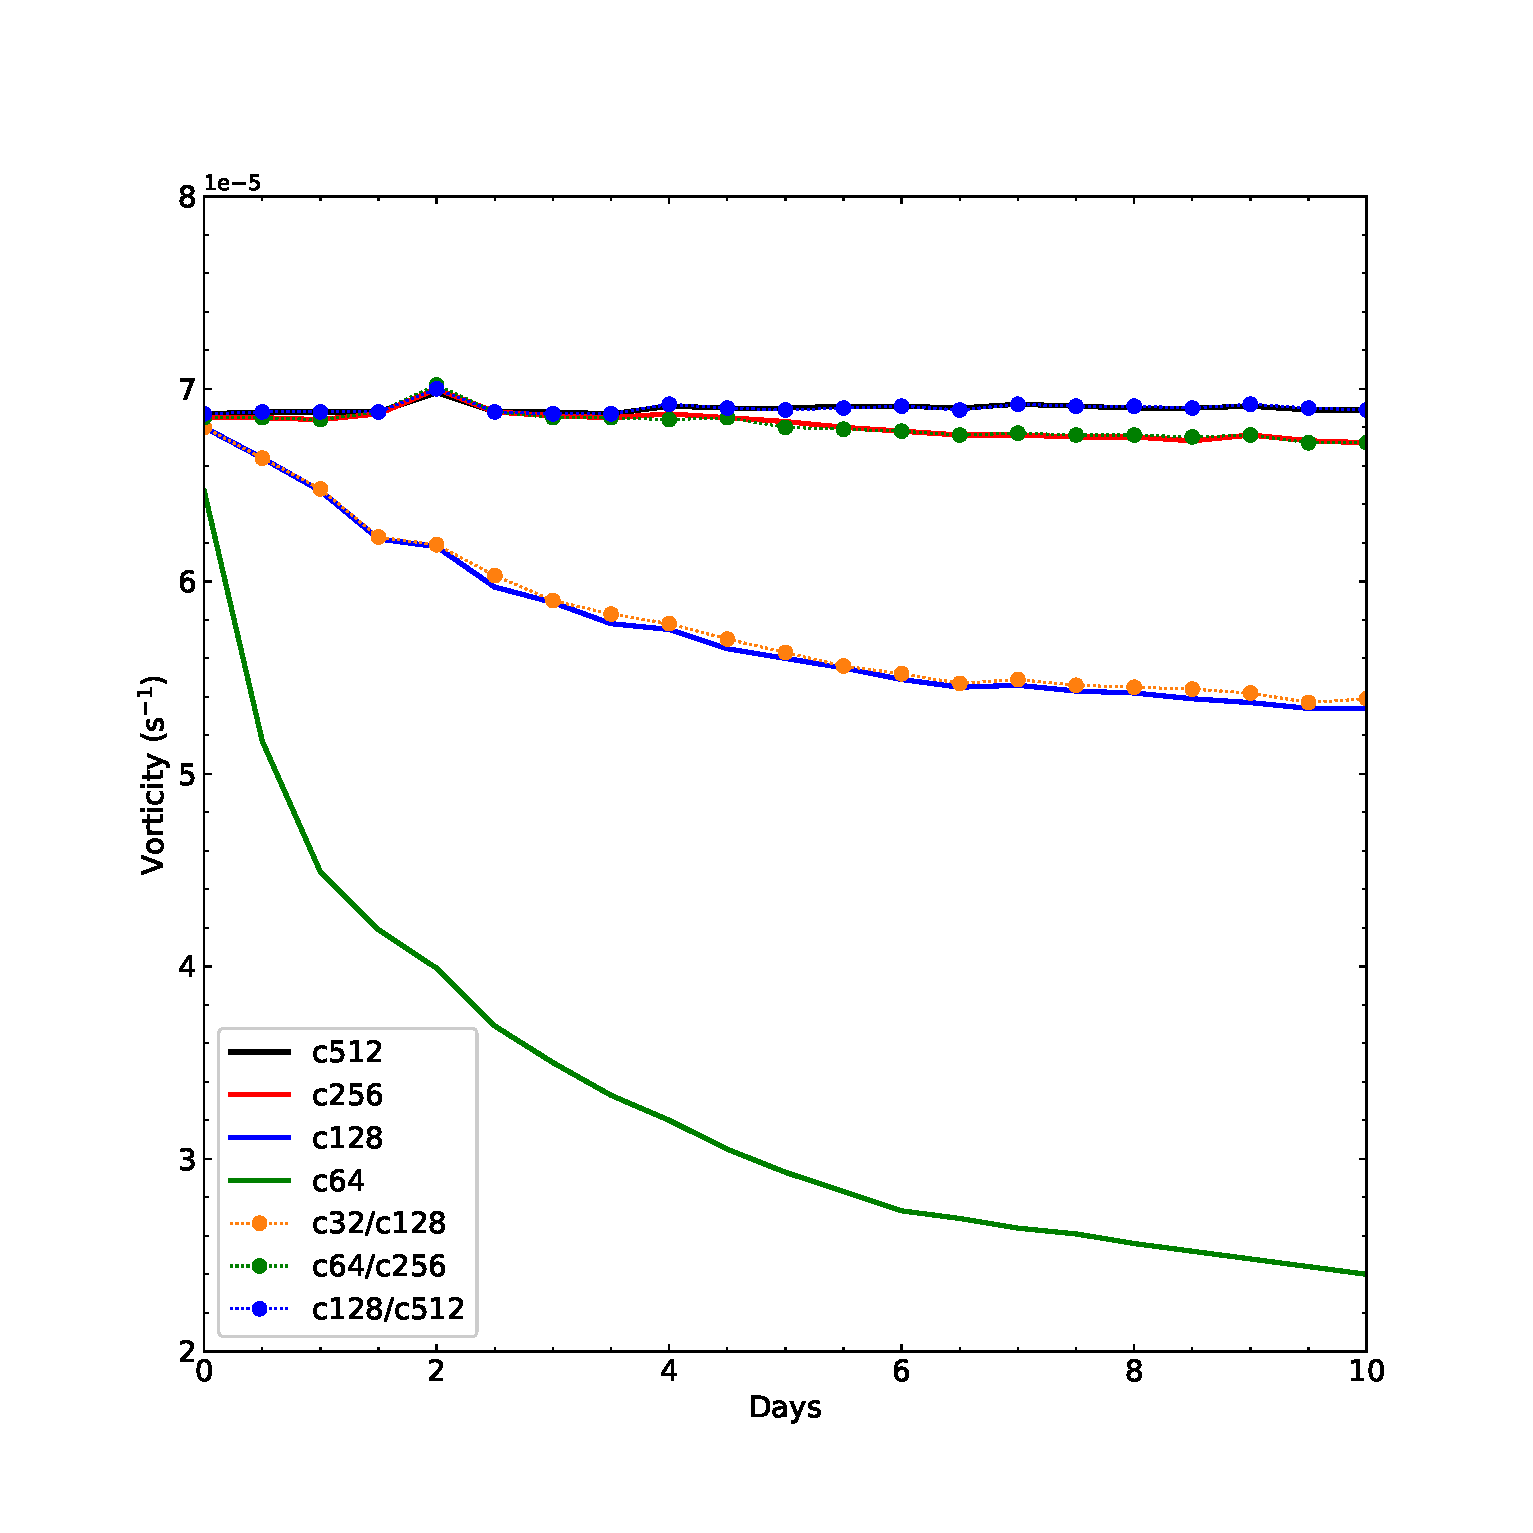
\includegraphics[width=\textwidth]{Chap3/modon_maxvort.eps}}
    \caption{10-day time evolution of the modons' maximum 
    vorticity for uniform and AMR runs.
}%
    \label{fig:modontevol}
\end{figure}

\subsection{Convergence tests}
We also use the modons test for some basic convergence tests
to assess the numerical methods. We compare
a series of uniform runs of varying resolutions and AMRs to
a uniform high-resolution reference solution. Since the modon test does not
have a known analytical solution, the c1024 uniform run in each scenario serves as
a reference solution. 
The normalized error measures for each run are
calculated via the traditional global error norms,
\begin{equation}
   \label{eq:l1_3d} L_1(h) = \frac{I\left[|h-h_\tau|\right]}{I\left[|h_\tau|\right]}
\end{equation}
\begin{equation}
   \label{eq:l2_3d} L_2(h) = \sqrt{\frac{I\left[(h-h_\tau)^2\right]}{I\left[h_\tau^2\right]}}
\end{equation}
\begin{equation}
   \label{eq:lmax_3d} L_\infty(h) = \frac{\max|h-h_\tau|}{\max|h_\tau|}
\end{equation}
where $h_\tau$ is the reference field and $I$ is a discrete approximation
to the global 3D integral given by
\begin{equation}
    \label{eq:globint_ed} I[x] = \sum_{\text{all cells } k} x_k V_k
\end{equation}
where $V_k$ denotes the volume of grid cell $k$.
With the finite-volume model, we expect fourth-order
convergence in the horizontal and second-order convergence in the vertical. However,
the time scheme is only second-order so the overall error convergence for any variable
tends towards second-order.

The 12-hour normalized errors as a function of grid resolution for density (left column) 
and vorticity (right column) are plotted in Fig. \ref{fig:largedterror}.
The runs depicted are uniform runs with resolution from c64 to c512
and three 1-level  x4 refinement AMR runs with c64, c128, and c256 base levels using the vorticity refinement criteria noted earlier.
These runs are implemented with the model's standard time step which fixes the CFL number at roughly $0.5$. With this,
the uniform c512 model has a time step of $\Delta t=20$ s, while the c64/c256 AMR run has a coarse fine step of $\Delta t =160$ s
and a sub-cycling time step of $\Delta t=40$ s for the c256 AMR level.  In the left column of Fig. \ref{fig:largedterror},
we observe second-order convergence in the $L_1$ (Fig. \ref{fig:largedterror}a) and $L_2$ (Fig. \ref{fig:largedterror}c) errors.
It is further reduced to first order for the $L_{max}$ in Fig. \ref{fig:largedterror}e.  Additionally, the AMR runs have roughly the same
errors as their base resolution uniform runs. No noticeable improvement is gained from the AMR; 
the vorticity tagging and refinement of only two localized areas is not 
expected to significantly improve global density errors.

We do observe improvements in the vorticity errors (Figs. \ref{fig:largedterror}b, d, and f) as a result of AMR. 
The c64/c256 AMR has higher errors than the uniform c256, but lower errors than the uniform c128 run 
in all three norms despite using roughly one-third the total number of grid cells in the c128 run.  The error improvement
is not as significant in the c256/c1024 AMR. This could be explained by the convergence of the solution at higher resolutions
resulting in diminishing returns for the benefits of AMR in improving global error \citep{lin2017colliding}.
Surprisingly, vorticity maintains a fourth-order convergence in the $L_1$ and $L_2$ error norm (Figs.  \ref{fig:largedterror}b and d)
and approximately third-order convergence in the $L_{max}$ norm (Fig.  \ref{fig:largedterror}f) even though it is not a prognostic variable, 
but derived from the momentum variables. By 24 hours, convergence does drop to second order for vorticity, 
and several days into simulation errors for all variables are first-order at best.

\begin{figure}
    \centerline{%
    \noindent
    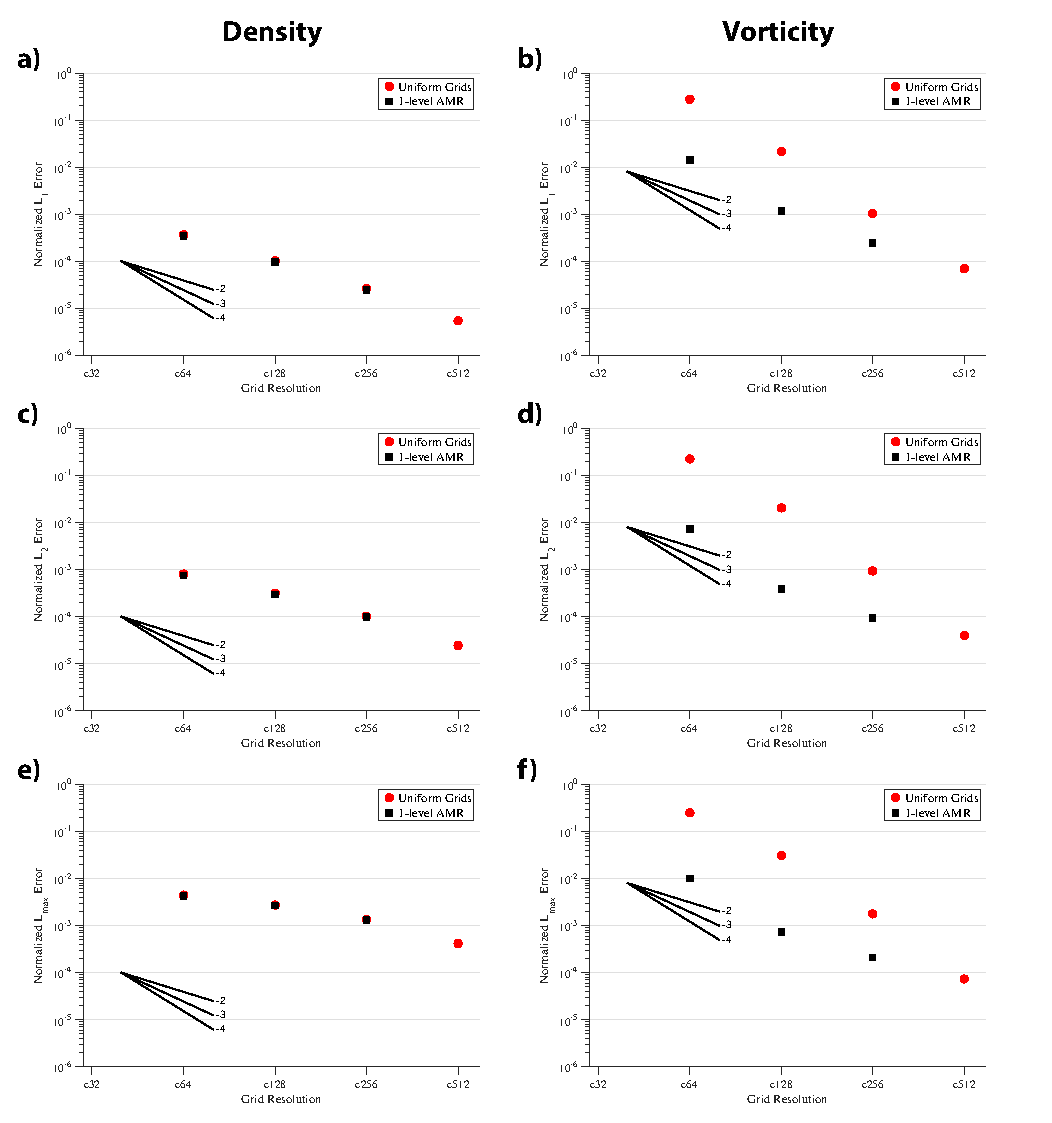
\includegraphics[width=\textwidth,height=\textheight,keepaspectratio]{Chap3/long_run_normerrs-01.eps}}
    \caption{The 12 hour $L_1$ (a)-(b), $L_2$ (c)-(d), and $L_{max}$ (e)-(f) normalized errors for
    $\rho$ density (left column) and vorticity (right column) with
    respect to the uniform c1024 run for uniform and 1-level x4 refinement 
    AMR runs. The AMR runs are plotted with respect to their base resolutions.
    These runs used the standard time steps which results in
    a CFL number of around $0.5$ for all resolutions.
}%
    \label{fig:largedterror}
\end{figure}

To assess if the horizontal discretization is achieving fourth-order accuracy,
we can work to minimize the temporal error source, so that the error is dominated 
by the spatial discretization. To this end, we perform a second convergence study comparing
c32 through c512 resolution uniforms with a c1024 reference run.
The time step in these runs is set to have CFL number of approximately $1/160$ in contrast to the $0.5$ in the previous study. 
We also only perform the error analysis at $t=160$ s so the temporal error does not have time to build up.
Note these runs were run with 32 vertical levels (all previous runs had 16 levels) to create a smoother vertical transition of variables.
The $L_1$, $L_2$, and $L_{max}$ errors are plotted in Fig. \ref{fig:smalldterror} for density \ref{fig:smalldterror}a, 
momentum in the $\alpha$ direction \ref{fig:smalldterror}b, and vorticity \ref{fig:smalldterror}c.
The uniform grid resolutions c64 and higher display fourth-order convergence in all 
three error norms for both $\rho u_\alpha$ momentum in Fig. \ref{fig:smalldterror}b
and vorticity in Fig. \ref{fig:smalldterror}c. The convergence rates of the three error 
norms for the density variable diverge (Fig. \ref{fig:smalldterror}a).  The  
second-order convergence of the $L_1$ error reduces to first-order at higher resolutions. 
The $L_2$ error is approximately third-order convergent at resolutions c128 and below, but also 
reduces to first-order at the highest resolutions. In contrast, the $L_{max}$ density error 
exhibits fourth-order convergence except at the coarsest c32 and c64 resolutions.
The variations in density convergence could be attributed to the test case 
is not fully balanced. The models has to rapidly adjust to cyclostrophic balance. 
The error distortions could rise from the adjustment processes affecting the density 
field, though this question warrants further investigation to confirm it is not an artifact of an
issue with the model numerics.

\begin{figure}
    \centerline{%
    \noindent
    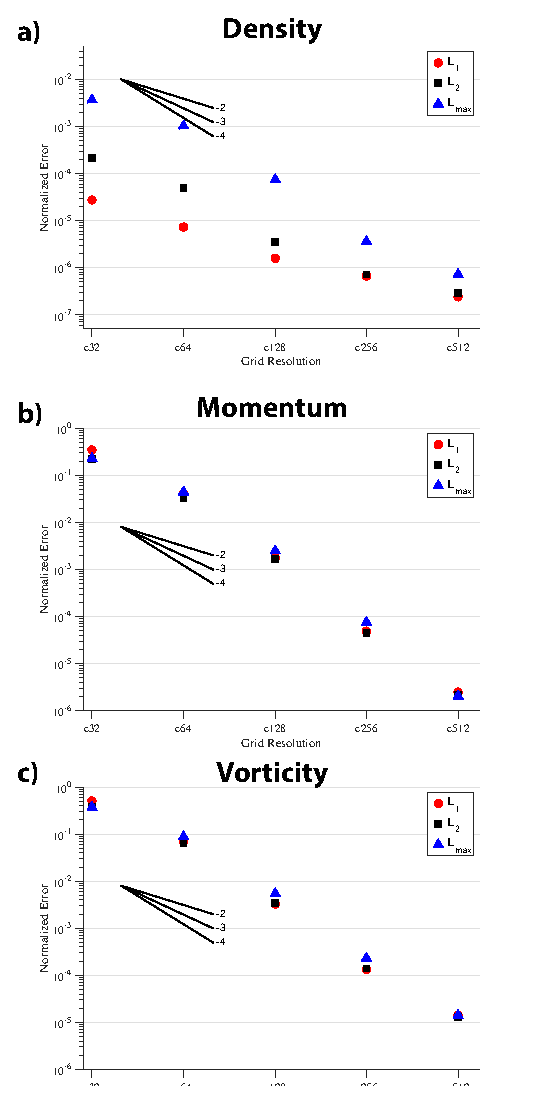
\includegraphics[height=.9\textheight]{Chap3/smalldt_normerrs-01.eps}}
    \caption{$L_1$, $L_2$, and $L_{max}$ normalized errors after $160$s 
    for (a) $\rho$ density, (b) $\rho u_\alpha$ momentum density, and (c) vorticity with
    respect to the uniform c1024 run. Small time steps are used which result in
     a CFL number of around $1/160$ for all resolutions.
}%
    \label{fig:smalldterror}
\end{figure}


\section{Idealized tropical cyclone}
\label{sec:tctest}

In the idealized TC test case by \cite{reed2012idealized}, a simple 
physics parameterization suit with the important driving mechanism of TCs
is added to the dycore. This causes
an initially weak vortex to rapidly intensify into a TC
and is a dynamic test case with real world applications.
We use the idealized TC to demonstrate AMR's effectiveness in tracking and resolving
the TC and asses how the physics forcing interacts with the AMR grid levels.
Its use is analogous to the 2D moist shallow water strengthening vortex test 
in Chapter \ref{chap:forcedsw}. A key focus area is the ability of the physics scheme
to handle changes in resolution, either at coarse-fine boundaries or when AMR is added
or removed. In addition, we are interested in assessing refinement criteria and AMR 
implementation timing effects on the evolution of the TC.

\subsection{Simple physics parameterization}
  The simple-physics parameterization suite of \cite{reed2012idealized}
  consists of three main mechanisms that drive tropical cyclone development.
  It implements a large-scale condensation mechanism that gets 
  triggered when the atmosphere becomes saturated. 
  The condensation scheme does not include a cloud stage, and it 
  instantaneously removes condensed moisture
  without any reevaporation at lower model levels. The 
  second component is a representation of the surface fluxes 
  that describe the interactions between the lower atmosphere and the ocean surface. 
  Specifically, it sets fluxes of horizontal momentum,
  sensible heat, and latent heat. The package assumes an aqua-planet surface with no topography
  and uniform sea surface temperatures. Finally, this scheme parameterizes boundary layer
  turbulence. For the Chombo AMR model, the physics time step is set to 16 minutes for all resolutions,
  comparable to the average physics time step
  used by models in \cite{reed2012idealized}. This time step is longer than 
  the dynamic time steps (40s to 6 mins, depending on resolution) used in this chapter.
  The frequency at which physics is called affects the evolution of the TC and
  is an area of further interest for AMR and the broad atmospheric modeling community.
  
\subsection{Idealized tropical cyclone}
  The initialization of the starting analytic vortex is
  described in detail by \cite{reed2011vortex}. The prescribed
  pressure, temperature, moisture, and velocity fields establish
  an initial vortex with initial maximum winds of $20$ m s$^{-1}$ located
  near the surface. The radius of maximum wind of roughly 250 km. The
  vortex is embedded in a background designed to
  mimic favorable tropical conditions.
  The background surface pressure is set to $p_0 = 1015$ hPa
  and the background wind at all vertical levels is zero.
  The model top height is set to 30 km and a stretched mapping is implemented
  in the height-based vertical coordinates.
  The mapping smoothly
  concentrates vertical levels closer to the surface to improve the resolution
  of the tropical cyclone and the physics processes that force it.

\begin{figure}
    \centerline{%
    \noindent
    \includegraphics[width=\textwidth]{Chap3/c256_intime-01.eps}}
    \caption{Snapshots of the tropical cyclone at day 3 (left), day 5 (middle), and day 10 (right)
    for the uniform c256 model run. (a)-(c) Surface pressure. (d)-(f) Wind speed at
    a height of 250 m. (g)-(i) Longitude-height cross-section of the wind speed through the center
    latitude of the vortex.
}%
    \label{fig:c256intime}
\end{figure}

   Figure \ref{fig:c256intime} depicts the evolution of the TC in 
   a c256 ($0.35^\circ$) uniform resolution run as it beta-drifts
   northwestward due to the Coriolis force over a period of ten days. The leftmost column shows 
   the surface pressure (Fig. \ref{fig:c256intime}a),
   the wind speed at 250m (Fig. \ref{fig:c256intime}d), and the vertical cross-section 
   of the wind speed (Fig. \ref{fig:c256intime}g). The middle column (Figs. \ref{fig:c256intime}b, e, and h)
   are the same plots for day 5, and the rightmost column (Figs. \ref{fig:c256intime}c, f, and i)
   depicts day 10.
   
   The c256 resolution is the highest resolution used for these simulations. As resolution
   increases, certain wave modes in the vertical components grow stronger and become unstable between
   the first and second day of the simulation. This time corresponds to the start of significant TC strengthening 
   which drives a rapid increase in vertical velocity at the TC's center. 
   The unstable modes add to this growth, eventually triggering CFL violations that stop the simulation.
   This instability can be mitigated by further decreasing the time step at higher resolutions. 
   However, such methods are not sustainable, as resolutions c512 or beyond require 
   time steps that are too small, making the simulation prohibitively costly to run. 
   Determining the causes of these unstable modes and possible solutions is an
   ongoing effort. For this reason, the highest resolution implemented for the TC test in uniform 
   or AMR mode is c256.


\subsection{AMR with the idealized TC}
In addition, to the uniform c256 run, we also ran uniform c64 and c128 runs.
We implemented four different refinement criteria for use in the AMR runs.
\begin{itemize}
    \item
        Tag 1 is a surface pressure threshold tag based on the
        absolute difference from the initial surface pressure $p_0=1015$ hPa. Refinement 
        is triggered where $|p_s - p_0| > 4$ hPa.
    \item
        Tag 2 is a relative vorticity threshold that refines where
        $|\zeta| >  2 \times 10^{-5} \mathrm{s}^{-1}$.
     \item
        Tag 3 is a relative vorticity threshold that refines where
        $|\zeta| > 1 \times 10^{-5} \mathrm{s}^{-1}$.
     \item
        Tag 4 is a surface pressure tag that refines where
        $|p_s - p_0| > 9$ hPa.
\end{itemize}
An overview of all simulations performed for this section, including the run resolutions and 
AMR refinement criteria used, is presented in Table \ref{tb:tcruns}.

\begin{table}[h]
  \caption{Brief description of all uniform and AMR runs performed for Sec. \ref{sec:tctest}.
  For each run the model resolutions, the refinement criteria (Tags 1 through 4), and the tagging variable are presented.
  Some of the AMR simulations have prescribed delays that prevent refinement from occurring until
  after a set time. That delay, in hours, is shown in the right most column. 
  The model resolutions (left most column) are presented in cubed-sphere coordinates ($cN$) with N
  being the number of cells along each panel edge.
  For the AMR runs, the resolutions for the multiple levels are given in the form c32/c128/c512, where the
  left most resolution is the base level's resolution and the subsequent 
  resolutions are for each level of AMR implemented.
  }
  \label{tb:tcruns}
  \begin{center}
 %    \resizebox{\textwidth}{!}{
  \begin{tabular}{lccc}
     \hline
     Run Resolution & AMR Criteria & Tagging Variable & Delay (hrs) \\
     \hline
     \hline
     c16/c64/c256 	& Tag 3	& Vorticity			& 0 \\
     c32/c128		& Tag 1	& Surface Pressure	& 0 \\
     c32/c128		& Tag 2	& Vorticity			& 0 \\
     c64			& - 		& - 				& - \\
     c64/c256		& Tag 1	& Surface Pressure	& 0 \\
     c64/c256		& Tag 2	& Vorticity			& 0 \\
     c64/c256		& Tag 3	& Vorticity			& 0 \\
     c64/c256		& Tag 4	& Surface Pressure	& 0 \\
     c64/c256		& Tag 1	& Surface Pressure	& 48 \\
     c64/c256		& Tag 3	& Vorticity			& 24 \\
     c64/c256		& Tag 3	& Vorticity			& 48 \\
     c128			& -		& -				& - \\
     c256			& -		& -				& - \\
     \hline
  \end{tabular}
%     }
  \end{center}
\end{table}

\begin{figure}
    \centerline{%
    \noindent
    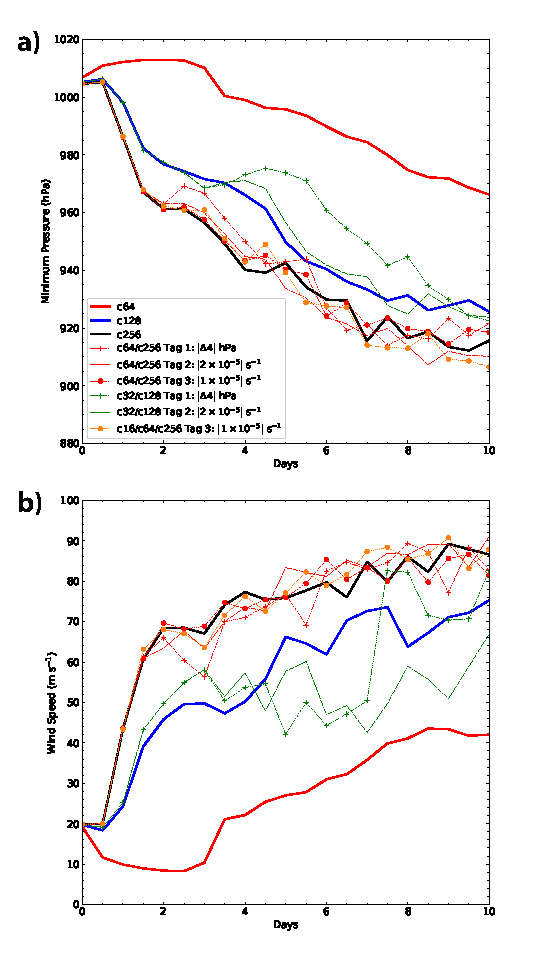
\includegraphics[height=.9\textheight]{Chap3/TC_amr_plots-01.eps}}
    \caption{Time evolution of the (a) minimum surface pressure and (b) maximum
    wind speed at 250m for three uniform runs and six AMR runs
    using various refinement criteria.
}%
    \label{fig:timeevolplots}
\end{figure}

Figure \ref{fig:timeevolplots} depicts the time evolution of the minimum surface
 pressure (Fig. \ref{fig:timeevolplots}a) and maximum wind speed at a height 
 of 250 m (Fig. \ref{fig:timeevolplots}b) for the three uniform runs and six AMR 
 runs using the first three tagging criteria. We observe that
the c256 run has a minimum surface pressure of around 920 hPa by day 10. This is
comparable to the strongest TC produced in \cite{reed2012idealized} using the 
simple physics scheme. Wind speeds in \cite{reed2012idealized} were calculated 
at 100 m, making direct comparisons difficult. In the uniform c64 run, the TC slowly
weakens initially. After day 3 it starts to strengthen but at a much slower rate 
than the higher resolution runs. By day 10, its maximum wind speed is less than half the 
c256 uniform run.
In \ref{fig:timeevolplots}, the four AMR runs that have a c256 level of refinement track the 
evolution of the uniform c256 TC closely. The two c32/c128 AMR runs also follow the uniform 
c128 run's progression but not as closely. Both the Tag 1 and Tag 2  c32 base AMR runs diverge 
markedly at several points during the ten days.
In all six AMR runs, the refinement threshold is met initially so that the TC is resolved by 
the highest level of AMR for the entire simulation.

\begin{figure}
    \centerline{%
    \noindent
    \includegraphics[width=\textwidth,height=\textheight,keepaspectratio]{Chap3/windspeed_amr-01.eps}}
    \caption{
    Day 10 snapshots of the horizontal wind speed at 250m for three uniform runs,
    (a) c64, (d) c128, and (g) c256, and the six AMR runs also depicted in 
    Fig. \ref{fig:timeevolplots}.
}%
    \label{fig:hwindsamr}
\end{figure}

\begin{figure}
    \centerline{%
    \noindent
    \includegraphics[width=\textwidth,height=\textheight,keepaspectratio]{Chap3/panel_vertwind_day10-01.eps}}
    \caption{
    Day 10 snapshots of the longitude-height cross-section
     of the wind speed through the center
    latitude of the vortex, for the same
    uniform and AMR runs as in Fig. \ref{fig:hwindsamr}.
}%
    \label{fig:vertwindsamr}
\end{figure}

The wind fields at a height of 250 m for all nine runs are shown in Fig. \ref{fig:hwindsamr}. 
The vertical cross-section of the wind fields centered around the
strongest vortex are plotted in Fig. \ref{fig:vertwindsamr}. From the uniform 
runs we observe increasing strength with increasing resolution
as well increasing compactness, a recognized sensitivity of simple physics 
\citep{reed2012idealized}. The TC strength and structure in the AMR runs compare well to
the corresponding uniform runs.  The main exception to this similarity is
the secondary vortex which spins up at the main TC's origin point. 
This TC is another resolution-sensitive feature, that is only produced in 
some models in \cite{reed2012idealized}.
In our simulation all three uniform runs have the secondary vortex developing, 
though it is only clearly defined in the c256 run. However, only half of the 
AMR runs develop this secondary vortex.
It develops in both Tag 3 AMR runs which have the broadest refinement, 
though it is fairly weak in Fig. \ref{fig:hwindsamr}h and much stronger than 
the c256 uniform run in the c64/c256 AMR run (Fig. \ref{fig:hwindsamr}i). 
Neither Tag 2 AMR runs develop the secondary vortex, and only the lower resolution 
c32/c128 surface pressure based AMR run (Fig. \ref{fig:hwindsamr}b) develops 
it. In Fig. \ref{fig:hwindsamr}b. the main TC is also significantly 
weaker than either the c128 uniform run (Fig. \ref{fig:hwindsamr}d) or the other 
c32/c128 AMR run (Fig. \ref{fig:hwindsamr}e) This main vortex is weakened by the
secondary vortex interfering with the main 
vortex's source of heat and moisture. This also explains the weakened eastern side of the
c64/c256 Tag 3's main TC, seen in Fig. \ref{fig:vertwindsamr}i. 
\cite{reed2012idealized} observed that small perturbations in the initial vortex structure 
led to noticeable spread in the evolution of the TC. So it is not
unexpected that differences in AMR grid locations can affect the evolution of the secondary vortex.
The tertiary vortex that appears in
the c16/c64/c256 AMR run (Fig. \ref{fig:hwindsamr}h) on the polar panel edge north of the main vortex
is a numerical artifact from the same AMR/panel edge issue observed in the modon tests.

\begin{figure}
    \centerline{%
    \noindent
    \includegraphics[height=.9\textheight]{Chap3/TC_delayed_plots-01.eps}}
    \caption{Time evolution of (a) minimum surface pressure and (b) maximum
    wind speed at 250m for three uniform runs and four AMR runs
    that do not have initial refinement over the vortex.
}%
    \label{fig:delayedplots}
\end{figure}

Initiating refinement at
the start of the simulation minimizes the growth of 
early coarse grid errors that carry over to the finer grids. 
In more realistic scenarios, a
distinct initial condition to tag on may not always be present. 
We are therefore interested in studying how the idealized TC and the simple physics mechanisms will
adjust to the addition of resolution when AMR is triggered a few 
days into the simulation rather than initially. 
The tag 4 criterion has a refinement threshold that is higher than the initial 
maximum surface pressure spread, so refinement is delayed
until the TC undergoes some strengthening on the coarse grid. Due 
to the high threshold though, the newly triggered AMR grid fails to sufficiently 
cover the whole TC for several additional days. To explore more refinement 
options, we implement an artificial delay to refinement. For the Tag 1 
and Tag 3 criteria, we manually shut off tagging in the model for either 24 
or 48 hours.  After that cut off, a broad area of refinement is applied over the TC.
Figure \ref{fig:delayedplots} shows the time evolution of the minimum surface
pressure (Fig. \ref{fig:timeevolplots}a) and maximum wind speed at a height 
of 250 m (Fig. \ref{fig:timeevolplots}b) for the four AMR runs.  The uniform 
runs are again plotted for comparison purposes. Figures \ref{fig:delayhwind} 
and \ref{fig:delayvertwind} depict the horizontal and vertical cross-sections of
the winds of the three AMR runs, respectively, with the uniform c256 run 
serving as a reference. 
The c64/c256 Tag 3 AMR run with a 48-hour delay was stopped at day 7 by 
the vertical velocity instability discussed at the beginning of this section, so
it is not pictured in these plots.

\begin{figure}
    \centerline{%
    \noindent
    \includegraphics[width=\textwidth,height=\textheight,keepaspectratio]{Chap3/day10_wind_amrdelayed-01.eps}}
    \caption{
    Day 10 snapshots of the horizontal wind speed at 250m for the three AMR runs
    that do not have initial refinement over the vortex. (a) Uniform c256, for reference.
    (b) c64/c256 using a tagging criterion of $|\Delta p| > 9$hPa. (c) c64/c256
    using Tag 3 with a 24-hour delay. (d) c64/c256 using Tag 1 with a 48-hour delay.
}%
    \label{fig:delayhwind}
\end{figure}

\begin{figure}
    \centerline{%
    \noindent
    \includegraphics[width=\textwidth,height=\textheight,keepaspectratio]{Chap3/day10_vertwind_amrdelayed-01.eps}}
    \caption{
    Day 10 snapshots of the jongitude-height cross-section
     of the wind speed through the center
    latitude of the vortex, for the same
    uniform and AMR runs as in Fig. \ref{fig:delayhwind}.
}%
    \label{fig:delayvertwind}
\end{figure}
 
The c64/c256 Tag 4 AMR run triggers refinement after three days. 
Figure \ref{fig:delayedplots} shows the drop in surface pressure and sharp 
jump in wind speed, however the AMR does not sufficiently cover the 
vortex resulting in the TC's strength fluctuating around the uniform c64 TC's level
despite refinement. In contrast, by day 10 the TC in the c64/c256 Tag 1 AMR 
run with a 48-hour delay has strengthened to c256 TC comparable wind speeds and surface pressure levels. Its
AMR is triggered after two and a half days but refines a broader area, capturing the whole TC. 
Once the refinement is triggered, the TC strengthens consistently until day 10, 
but the increase is not as rapid as the other delayed AMR runs.
This is also true in comparison to  the
initial strengthening of the c128 and c256 uniform runs. 
The TCs in the two delayed Tag 3 AMR runs follow similar trajectories.
After the delay, refinement is immediately triggered over the whole TC and the surrounding area. The 
TC undergoes an abrupt transition that temporarily distorts the vortex structure for approximately 24 hours and causes it to rapidly strengthen.
The evolution of the c64/c256 Tag 3 AMR run with the 24-hours delay mimics 
the rapid strengthening of the uniform c256 TC, merely a day behind.  By day 6, 
the minimum surface pressure and wind speed in the Tag 3 AMR 
and the c256 uniform runs are approximately the same.
At day 10, Figs. \ref{fig:delayhwind} and \ref{fig:delayvertwind} 
shows that both the Tag 1 and Tag 3 delayed
runs have TCs comparable to the uniform c256 TC. The c64/256 Tag 3 delayed run
even captures the development of the 
secondary vortex (Fig. \ref{fig:timeevolplots}c).
The processes in the evolution of the high resolution TC can still be 
triggered in AMR runs that do not have high levels of refinement initially.
These AMR runs demonstrate a time window during which the TC can undergo rapid strengthening
and evolve into a vortex comparable to the TC from the uniform high resolution run.

\section{Conclusions}
\label{sec:conclusion3}

In this chapter, we used the non-hydrostatic finite-volume Chombo AMR dycore
and demonstrated its AMR characteristics for idealized 3D atmospheric flows on the sphere.
 We implemented two test cases: the colliding modons
test, in the dry dycore and the idealized TC test with an added simple moist physics parameterization package.
In the modon test, AMR functioned as expected. It was able to tag, refine, and follow the modons
and it effectively reduced the global vorticity errors.
The error convergence properties met our expectations given 
the implemented numerical schemes and the current status of the model.
However, a few notable results trigger the need for further investigations.
Several stability problems were observed in both test cases that need to
be better understood and corrected.

In the idealized TC test, the AMR runs were able to effectively reproduce results from uniform high resolution runs.
The physics scheme was able to function effectively over multiple levels of refinement. No noise
or instabilities were observed at coarse-fine boundaries, though some
 numerical artifacts were observed on polar panel edges. 
Several aspects of the TC's evolution were
sensitive to the tagging criteria and AMR coverage such as the generation of the secondary vortex.
Having  AMR levels applied initially is the most effective way of improving results.
However, the delayed AMR tests demonstrated that the TC can still 
undergo the same strengthening processes as high resolution runs once refinement is triggered.
There is a narrow window of flexibility, in which the triggering of AMR allows the TC in the AMR 
run to catch up to the results in the high resolution uniform run.
The most promising refinement technique is a combination of some initial 
refinement and AMR. The initial refinement limits error growth at the 
base resolution and ensures that the model can resolve the feature of interest. 
Additional AMR level then enable the feature to then be fully resolved.




 
  \chapter{Conclusion}
 \label{chap:conclusion}
 Complex multi-scale atmospheric phenomena, like tropical 
cyclones, challenge conventional weather and climate models, 
which use relatively coarse uniform-grid resolutions to cope with 
computational costs. Adaptive Mesh Refinement (AMR) techniques 
mitigate these challenges by dynamically and transiently placing high-resolution grids 
over salient features, thus providing sufficient local resolution while 
limiting the computational burden. 
This thesis explores the development of AMR within a new 
non-hydrostatic, finite-volume dynamical core and demonstrates its 
effectiveness in improving model accuracy and its ability to resolve 
multi-scale features. The AMR dynamical core is implemented in a 
hierarchy of models of increasing complexity, from an idealized 2D 
shallow water configuration to the non-hydrostatic 3D equation set 
with subgrid-scale physics parameterization schemes. The research explores 
effective refinement practices and assesses the benefits achieved 
with increased dynamic refinement. It is shown that AMR is a 
powerful modeling approach that bridges the resolution gap for 
extreme weather events.

In Chapter \ref{chap:basicsw} we utilized a fourth-order
finite-volume model on a cubed-sphere grid, which is adaptive in both
space and time, to demonstrate the effectiveness of the AMR in resolving
and tracking chosen features of interest while maintaining large-scale
smooth flows.  Using selected shallow-water and advection test cases, we
evaluated the AMR's ability to track and resolve features of interest
without creating distortions or numerical noise in the large-scale
smooth flows at the interfaces between meshes. 
Static and dynamic refinements were analyzed to determine the 
strengths and weaknesses of AMR in both complex flows with small-scale
 features and large-scale smooth flows. The different test cases required 
 different AMR criteria, such as vorticity, height, or gradient-based thresholds, 
 in order to achieve the best accuracy. The simulations showed that the 
 model can accurately resolve key local features without requiring global 
 high-resolution grids. The adaptive grids are able to track features of interest 
 reliably without inducing noise or visible distortions at the coarse-fine interfaces. 
 Furthermore, the AMR grids keep any degradations of the large-scale smooth flows to a minimum.
 
In Chapter \ref{chap:forcedsw} we implemented two different forcing schemes designed to 
mimic the effects of moisture in the atmosphere within the 2D AMR
shallow water system. The first moist physics
framework added water vapor variable and models convection
as a mass sink triggered by saturation. We implemented a
strengthened vortex test case with this setup.  In the second
forcing framework, a more complex moisture representation
is used, consisting of vapor, cloud, and rain variables.
The effects of moisture were coupled to the momentum equations
through a potential temperature variable, linked to
the moisture variables through latent heat. This physics
scheme was used with a barotropic instability test case. 
With both forcing systems and test cases, we observe the evolution
 of features of interest at various resolutions and 
with different refinement strategies. 
We also investigated the AMR's effect on the physics 
forcing as grid resolutions changed.
These simulations can help develop AMR tagging strategies and refinement criteria.
Both sets of simulations showed that the starting resolution must be
able to adequately resolve the feature of interest to maximize
the effectiveness of AMR. AMR cannot remove the errors
caused by coarse grids before refinement begins. Additional refinement with
AMR beyond the base grid level did improve the model, especially
with regards to the small-scale vorticity features in the strengthening vortex test case.
To obtain such early refinement with AMR, the tagging
criteria must be tailored to properties that are uniquely associated
with the origins of the feature of interest. This is difficult even in these 
idealized shallow water systems.

In Chapter \ref{chap:3dmodel}, we implemented AMR in 
the non-hydrostatic finite-volume Chombo AMR dycore
and tested it for idealized 3D atmospheric flows on the sphere. 
We used two test cases: the dry dycore colliding modons
test and an idealized TC test with a simple moist physics parameterization scheme.
In the modon test, AMR functioned as expected. It was able to tag, refine, and follow the modons,
and the added resolution  effectively reduced global the vorticity errors.
The error convergence properties met our expectations given the numerical 
schemes used and the current status of the model. However, a
 few results triggered the need for additional in-depth examinations.
Several stability problems were observed in both test cases 
that need to be better understood and addressed.

In the idealized TC test, the AMR runs were able to effectively reproduce results from uniform high resolution runs.
The physics scheme was able to function effectively over multiple levels of refinement. No noise
or instabilities were observed at coarse-fine boundaries, though some
 numerical artifacts were observed on polar panel edges. 
Several aspects of the TC's evolution were
sensitive to the tagging criteria and AMR coverage such as the generation of the secondary vortex.
Having  AMR levels applied initially is the most effective way of improving results.
However, the delayed AMR tests demonstrated that the TC can still 
undergo the same strengthening processes as high resolution runs once refinement is triggered.
There is a narrow window of flexibility, in which the triggering of AMR allows the TC in the AMR 
run to catch up to the results in the high resolution uniform run.
The most promising refinement technique is a combination of some initial 
refinement and AMR. The initial refinement limits error growth at the 
base resolution and ensures that the model can resolve the feature of interest. 
Additional AMR level then enable the feature to then be fully resolved.
For example, in tracking and resolving TCs in a realistic climate simulation, 
a static region of refinement
could be placed over regions of cyclogenesis. Any storms that
develop could be further refined and followed with AMR as they traverse
and exit the region of static refinement.


\subsection{Collaborations}
This research has built collaborations between the University of Michigan (UofM), the 
Applied Numerical Algorithms Group (ANAG) at the Lawrence Berkeley National Laboratory (LBNL), and
the University of California, Davis (UC Davis). In particular, direct contributors to 
the research contained in this thesis include 
Christiane Jablonowski (UofM), Hans Johansen (LBNL), 
Peter McCorquodale (LBNL), Phillip Colella (LBNL), and Paul Ullrich (UC Davis).

\subsection{Future Work}

\textbf{AMR dycore development:}
Additional effort is required in implementing, validating, and improving AMR within GCMs.
Use of AMR in a 3D non-hydrostatic dycore is a relatively recent application. 
Further development includes the creation
of more complex models with realistic physics schemes, with
the goal of running aqua-planet simulations with full-physics schemes. 
Implementing vertical refinement with AMR is another algorithm development focus.
With an AMR non-hydrostatic model, grid resolutions on the order of 1km or finer are feasible.
At these resolutions, the aspect ratios between the horizontal and vertical lengths of a grid cell 
can be come highly skewed.  The addition of more vertical cells would alleviate this issue, and 
increase vertical resolution. 

 \vspace{6pt}
\textbf{Scale aware subgrid physics parameterizations:}
The effectiveness of VRGCMs is limited by the sub-grid physical parameterizations used to
approximate atmospheric features including radiation and sub-grid scale process like convection, 
clouds, and turbulence that cannot be resolved by the dycore.
In adaptive schemes, the subgrid-scale parameterizations need to be able to adjust for changes in scale.  
A model will need to be able to phase out certain subgrid-scale processes, like deep
convection, as resolution is increased and these processes are resolved on the actual mesh.
One novel research avenue is the application of artificial intelligence to aid in the development of
these scale-aware physics schemes.

\vspace{6pt}
\textbf{AMR and topography:}
Choosing an effective method to handle topography is a challenging endeavor for any model. 
The question of smoothing always arises as very steep topological gradients can cause issues 
for the vertical coordinates and create numerical noise.  AMR faces the additional hurdle of how to deal 
with topography when the grid is refined over it.  Literature on this subject is rather sparse, but there are 
several possible methods of approaching this issue.  One traditional method is to merely interpolate the
 existing coarse-grid topography to the new grid cells.  This method, though preserving monotonicity, will not necessarily 
 improve orographic representation as it cannot make mountains taller, valleys deeper, or gradients steeper.   
 A second method would be to actually alter the topographic features making them more pronounced 
 and even steeper or taller when the grid is refined.  The topography can then be smoothed down for 
 coarse grids and merely updated back to the high-resolution version when AMR refines it.  
 Such a method provides a more realistic orographic representation but could be numerically 
 unsound, causing air mass conservation issues and creating large gravity waves.  A third method 
 is to merely keep a static refinement mesh over large topographic features, though this 
 could be computationally inefficient.
 
 
%\startappendices
% \appendix{Vertical mapping for the idealized tropical cyclone test case}
% \label{app:vertmap}
% \input{Appendices/Vert_mapping}


\startbibliography
 \begin{singlespace} % Bibliography must be single spaced
  \bibliography{all_references}   % Use the BibTeX file ``References.bib''.
 \end{singlespace}

% An external Abstract that can be printed at the end of the document, 
% for separate submission to Rackham. Comment it out when not needed. - jg
%\startextabstractpage
%{The Title of Your Dissertation}{Your Name}{Chair: Albert Einstein}
%Complex multi-scale atmospheric phenomena, like tropical 
cyclones, challenge conventional weather and climate models, 
which use relatively coarse uniform-grid resolutions to cope with 
computational costs. Adaptive Mesh Refinement (AMR) techniques 
mitigate these challenges by dynamically and transiently placing high-resolution grids 
over salient features, thus providing sufficient local resolution while 
limiting the computational burden. 

This thesis explores the development of AMR, a technique that 
has been featured only sporadically in the atmospheric science 
literature, within a new nonhydrostatic, 
finite-volume dynamical core and demonstrates AMR's effectiveness in 
improving model accuracy and ability to resolve multi-scale features. 
This high-order finite-volume model implements adaptive refinement in both space and 
time on a cubed-sphere grid using a mapped-multiblock mesh technique developed with
the Chombo AMR library. The AMR dynamical core is implemented in a hierarchy of
models of increasing complexity, from an idealized 2D shallow water configuration 
to the nonhydrostatic 3D equation set with subgrid-scale parameterizations schemes. 
AMR's numerical accuracy, computational efficiency, and ability to track and resolve
multifaceted and evolving features are assessed with
a variety of existing and new test cases, implemented within each model iteration.

Both static and dynamic refinements are analyzed to 
determine the strengths and weaknesses of AMR in both 
complex flows with small-scale features and large-scale smooth flows.
The different test cases required different AMR criteria, such 
as vorticity, or minimum pressure based thresholds, 
in order to achieve the best accuracy for cost. Simulations show 
that the model's AMR can accurately resolve key local features in 
both shallow water and 3D test cases without 
requiring global high-resolution grids, as the adaptive grids are able 
to track features of interest reliably without inducing noise or visible 
distortions at the coarse-fine interfaces. Furthermore, the AMR grids 
keep degradation of the large-scale smooth flows to a minimum.
2D and 3D physics parameterizations are able to 
function effectively over multiple levels of refinement, though
the parameterizations are sensitive to grid resolution.

AMR is most effective when refinement is triggered early 
or when the base uniform resolution can partially 
resolve the features of interests. Very coarse base resolutions
lead to large initial errors that cannot be overcome by AMR.
However, the addition of refinement later in the simulation still results
in significant improvements, especially in 
resolving small-scale features. The research showed that
flow properties, such as strong gradients or rainbands, 
can be sensitive to small changes in AMR
criteria. These may delay the onset of the refinement
 or alter the shape of the refined area, which
impacts the evolution of the flow. With coarse 
base resolutions, the tagging criteria must 
therefore be uniquely tailored to capture the early 
growth phases of the feature of interest.
A promising refinement technique is a combination of 
some initial refinement and AMR. 
The initial refinement limits error growth at the base 
resolution and ensures that the model can 
resolve the feature of interest. Overall,
AMR is shown to be a powerful modeling approach 
that bridges the resolution gap for extreme weather events.
%\label{ExtAbstract}

\end{document}